%The following line prevents the headers and the \begin{document}\end{document}
%from being executed in the individual files.
\def\whole{}
\documentclass[leqno]{book}
\input style-for-curves.sty
\usepackage{hyperref}
%\input header.tex

%\documentclass{cambridge7A}
%\usepackage{ag2}
\usepackage{xcolor}
%\usepackage{mtpro2}
%\usepackage{times}
%\usepackage{hatcher}
%\usepackage{msribib,local}
%\usepackage{geompsfi}

\errorcontextlines=1000

%\usepackage{makeidx}
\makeindex
% \index{word} in the doc; \index{variety!algebraic} gives variety, algebraic
% PUT a % after each \index{***}

\overfullrule=5pt
\catcode`\@\active
\def@{\mskip1.5mu} %produce a small space in math with an @

\title{Personalities of Curves}
\author{\copyright David Eisenbud and Joe Harris}
\begin{document}
\maketitle

\pagenumbering{roman}
\setcounter{page}5
\pagenumbering{arabic}
\tableofcontents
%\includeonly{01-Overture, 04-ChowGroups }
%\def\all{toc,out1,chern,out2,lefschetz,out3,bib,ind, out1a}
%\includeonly{\all}

\input header.tex

\setcounter{chapter} {-1}
\chapter{Basic Questions}

\fix{The following is more material for a preface than a preface...}
\begin{center}
\emph{I'm very well acquainted, too, with matters mathematical,\\
I understand equations, both the simple and quadratical,\\
About binomial theorem I am teeming with a lot o' news,\\
With many cheerful facts about the square of the hypotenuse.}

---Gilbert and Sullivan, Pirates of Penzance, Major General's Song


\emph{Be simple by being concrete. Listeners are prepared to
accept unstated (but hinted) generalizations much more than they are able, on the spur of the moment, to
decode a precisely stated abstraction and to re-invent the special cases that motivated it in the first place. }

--Paul Halmos, How to Talk Mathematics

\emph{Another damned thick book! Always scribble, scribble, scribble! Eh, Mr. Gibbon?} --- \scriptsize{Prince William Henry, upon receiving the second  volume of The History of the Decline and Fall of the Roman Empire from the author.}
\end{center}


The most primitive objects of algebraic geometry are affine algebraic sets---subsets of $\RR^{n}$ or $\CC^{n}$ defined by the vanishing of polynomial functions---and the maps between them. But already in the first half of the 19th century geometers realized that there was a great advantage in working with varieties in complex projective space, treating affine varieties as projective varieties minus the intersection with the plane at infinity and real varieties as the fixed points of the complex involution. One sees this in the simplest examples: the ellipses, hyperbolas and parabolas in the real affine plane are all the same in the complex projective plane; the difference is only in how they intersect the line at infinity. A difficulty with the projective point of view is that on a connected projective variety there are no non-constant functions at all (reason: a function on a projective variety is a map to the affine line; since the image of a projective variety is again projective, the image would be a single point.) 

Starting with Riemann in the 1860s and culminating in the scheme theory of Grothendieck in the 1950s, algebraic varieties were treated in a way independent of any embedding: An algebraic variety is is a topological space with a sheaf of locally
defined polynomial functions. Many interesting aspects of geometry have to do not with single abstract varieties, but with maps between them, and in particular with embeddings in projective spaces. In general, maps between varieties can be described by their graphs, which are again varieties.  But for the special case of maps to projective spaces, the theory of \emph{linear series} is usually a more convenient description. The collection of all linear series on a variety reflects some of its best understood invariants. 

The basic objects of study in this book are smooth, connected projective algebraic curves over an algebraically closed field of characteristic 0, which we take to be the complex numbers $\CC$. Though we assume that the reader has been exposed to this theory in some form before, perhaps from Chapter IV of Hartshorne's {\it Algebraic Geometry}, we will review the elements  in the form we will use. 

\section{Algebraic Curves and Riemann Surfaces}

These objects can be viewed in two distinct but equivalent ways: as \emph{compact Riemann surfaces}, or compact complex manifolds of dimension 1; and as \emph{smooth projective algebraic curves over $\CC$}. (Here, when we use the term projective variety, we mean a variety isomorphic to a closed subset of projective space, not a variety with a specified embedding in $\PP^n$.) There are advantages to each point of view---the complex analytic point of view is more concrete, and requires relatively minimal amount of preliminaries; the algebraic point of view is substantially broader. 

First, if $C \subset \PP^n$ is a smooth, projective curve over $\CC$, then it is a submanifold of complex projective space, and so a Riemann surface. 
\fix{discuss geometric genus vs. arithmetic genus here?}

The other direction---going from a compact Riemann surface $C$ to a smooth projective curve over $\CC$, or equivalently embedding $C$ as a complex submanifold of $\PP^n$, after which Chow's theorem says that it is in fact a projective variety---is much deeper. The first, and hardest step is to show that a compact Riemann surface admits a nonconstant meromorphic function $f:C \to \CC$, and the corresponding statement is not true in higher dimensions. The function $f$ can be viewed as
a rational map $f': C\to \PP^{1}$. The next step is to see that the field $K(C)$ of all meromorphic functions
on $\CC$ is a finite extension of the field of rational functions on $\PP^{1}$; the sheaf of regular functions on $C$ is then the integral closure of the sheaf of regular functions on $\PP^{1}$ in $K(C)$.

Though equivalent for curves defined over $\CC$, these approaches have a very different flavors. For example,
given a map  $f: C\to C'$ from a smooth curve $C$ to a possibly singular curve $C'$ that is generically one-to-one, we can reconstruct $C$.
From the algebraic point of view this can be done by \emph{normalization}, or more concretely by blowing up the singular points of $C'$. From the analytic point of view, we can use the Weierstrass preparation theorem, which implies that there is the neighborhood $U$ of any point $p\in C'$ such that the punctured neighborhood $U \setminus p$ is isomorphic to a disjoint union of punctured discs; and $C$ is obtained by completing this to the corresponding disjoint union of discs.

\section{Families of varieties}

\subsection{Hilbert schemes}

\subsubsection{Definition, universal property; construction}

\subsubsection{examples of hypersurfaces and linear spaces}

\subsubsection{tangent space}

\subsubsection{Fundamental problem: irreducible components of Hilb parametrizing smooth curves and their dimensions}

\begin{example}
conics in $\PP^3$ (refer to 3264)
\end{example}

\subsection{Moduli spaces of curves}

\subsubsection{basic properties of $M_g$ (coarse rather than fine; fine over automorphism-free curves)}

\subsubsection{dimension $3g-3$, irreducible}  (just statements, w/ref to Harris-Morrison)



\section{Moduli problems}

It is a fundamental aspect of algebraic geometry that the objects we deal with often vary in families, and can often be parametrized by a ``universal" such family. For example, the family of plane curves of degree $d$ may be thought of as the projective
space $\PP(H^{0} \sO_{\PP^{2}}(d))$, and similarly with hypersurfaces in any projective space. This notion of objects varying with parameters underlies many of the constructions and theorems we will discuss. 

\subsection{What is a moduli problem?}

Briefly, a \emph{moduli problem} consists of two things: a class of objects, or isomorphism classes of objects; and a notion of what it means to have a \emph{family} of these objects parametrized by a given scheme $B$. To make this relatively explicit, the four main examples of moduli problems we'll be discussing here are:

\begin{enumerate}
\item  smooth curves: objects are isomorphism classes  of smooth, projective curves $C$ of a given genus $g$. A family over $B$ is a subscheme $\cX \subset B \times \PP^r$, smooth, over $B$, whose fibers are curves of genus $g$.

\item the Hilbert scheme: objects are subchemes of $ \PP^r$ with a given Hilbert polynomials. A family  is a subscheme $\cX \subset B \times \PP^r$, with $cX$ flat over $B$, whose fibers have the given Hilbert polynomial. We will be interested in the case of Hilbert polynomial $p(m) = dm-g+1$ and the open subscheme corresponding to smooth projective curves $C \subset \PP^r$ of degree $d$ and genus $g$.

\item effective divisors on a given curve: objects are effective divisors of a given degree $d$ on a given smooth, projective curve $C$. A family over $B$ will be a subscheme $\cD \subset B \times C$ flat over $B$, with fibers of degree $d$

\item invertible sheaves on a given curve $C$: objects are invertible sheaves of a given degree $d$ on $C$. A family over $B$ is an invertible sheaf on the product $B \times C$ whose restriction to each fiber over $B$ has degree $d$. We identify two such sheaves if they differ by tensor product with an invertible sheaf pulled back from $B$.
\end{enumerate}

Given a moduli problem, our goal will be to describe a corresponding \emph{moduli space}. By this we mean a scheme $M$ whose points are in \emph{natural} one-to-one correspondence with the objects in our moduli problem. This will realize the objects of the moduli problem as the points of the underlying set of the scheme $M$.

If the moduli space in question and the base of the family are varieties, then the crucial condition that the correspondence be \emph{natural} is simple to express: that given a family of the objects in our moduli problem over a variety $B$, the map from underlying set of $B$ to the underlying set of $M$ taking each fiber
to the corresponding point of $M$ should be a morphism of varieties.  But in the world of schemes the set-theoretic mapping does not determine the morphism of schemes (think, for example, of the morphisms from $\Spec(\CC[x]/x^{2})$ into the plane with the closed point mapping to the origin. The situation is even worse when the moduli space itself is not a variety.)

To deal with the general case, we recast the naturality condition in functorial terms. We observe first that a moduli problem defines a functor $\cM$ from the category of schemes to the category of sets: the value of the functor at a scheme $B$ is the set of families of objects parametrized by $B$; a morphism $B' \to B$ of schemes gives rise, via pullback, to a map of sets $\cM(B) \to \cM(B')$. We define a \emph{fine moduli space} for the moduli problem to be a scheme $M$ that represents this functor, in the sense that there is an isomorphism of functors
$$
\cM \to {\rm Mor}(\bullet, M)
$$
In other words, for every scheme $B$ we have a bijection between families of our objects over $B$ and morphisms from $B$ to $M$. In particular, applying this to $B = \Spec \CC$, we have a bijection between the set of objects and the closed points of $M$; and for any family over an arbitrary scheme $B$, the map from $B(\CC)$ to $M(\CC)$ sending each closed point  $b \in B$ to the point in $M(\CC)$ corresponding to the fiber over $b$ is the underlying map of a morphism $B \to M$ of schemes.

If a fine moduli space for a given problem exists at all, then Yoneda's Lemma shows that it is unique up to a unique isomorphsm. This is a real problem: there is no fine moduli space for the first and most important of the examples above---the isomorphism classes of smooth curves---though there is for the others. We'll defer the discussion of why this is, and what we can do about it, until Chapter~\ref{Moduli chapter}.

Looking ahead, we'll discuss the third and fourth example in Chapter~\ref{}, where we'll describe the moduli spaces for effective divisors of given degree $d$ on a given curve $C$ (the symmetric powers of the curve) and for invertible sheaves of a given degree on $C$ (the \emph{Jacobian} and \emph{Picard variety} of $C$). These, as we'll see, are smooth, irreducible projective varieties of dimensions $d$ and $g$ respectively.

We'll take up the moduli space $M_g$ of smooth curves in Chapter~\ref{Moduli chapter}, where we'll see that this space (or rather the closest approximation to it we can cook up) is irreducible of dimension $3g-3$ for $g \geq 2$, though not smooth or projective.

Finally, the Hilbert scheme will be described (to the extent that we can!) in Chapter~\ref{HilbertSchemesChapter}; this will turn out to be much wilder and more varied in its behavior than any of the above.




%\section{Outline}
% \begin{enumerate}
%
%\item Background \begin{enumerate}
%
%\item Lasker's Theorem (complete intersections are unmixed) -- sometimes incorrectly called ``$AF+BG$''
%state ci implies unmixed; prove by $H^1$ of line bundle.
%
%\item B\'ezout and the  weak B\'ezout (ex 8.4.6 in Fulton).
%B\'ezout via Koszul complex, at least in codim 2.
%
%
%
%
%\end{enumerate}
%\item Basics of curves (corresponds to material in Hartshorne Ch 4, sects 1,2,4(?)---all except elliptic curves and ``classification")
%
%\begin{enumerate}
% \item Discussion of genus of smooth curves. Riemann-Roch. Hilbert coefficient.
%
%\item Divisors and maps; canonical divisor -- cotangent bundle; canonical map as example
%Exercise: Projections from on and off a curve
%
%\item canonical series is bpf, $2g+1$ is very ample. Canonical Curves and geometric RR
%
%\item Adjunction formula for curves in a surface (Quote from Hartshorne)
%
%\item Clifford, including strong form, canonical series is va except in hyperelliptic case.
%
%\item Riemann-Hurwitz (pull back a differential form)
%
%\end{enumerate}
%%\end{enumerate}
%
%\item Families of curves and Brill-Noether theory
%\begin{enumerate}
%\item Families. Define families. discuss "good and bad" families. example: symmetric product. example: plane curves of degree d. family of line bundles on a curve (or a family of curves.)
%
%\item How many curves of genus g are there? Informal discussion of moduli. 
%\item Cheerful fact about the existence of  Hilbert scheme, $M_g$, and $\overline M_g$, meaning of the phrase ``coarse moduli space''.
%
% \item Lowest degree of a covering of $\PP^1$?
% \item Lowest degree of a plane model?
% \item Lowest degree of an embedding?
% \item Number of forms of of degree d vanishing on the curve---ideals of the embeddings, Hilbert Functions.
%\end{enumerate}
%
%\item Personalities
%\begin{enumerate}
%\item $g=0$: rational curves as projections of rational normal curves. Rational quartic in $\PP^3$. Mention Set-Theoretic Complete Intersection problem.
%\item $g=1$. Wonderful subject; refer to somewhere else. Plane cubic, quartic in $\PP^3$, state that an elliptic quintic is Pfaffian (give proof??).
%\item $g=2$. Canonical map to $\PP^1$. Embedding in $\PP^3$ as $(2,3)$ on a quadric, ideal is 1 quadric, 2 cubics.
%\item $g=3$. Plane quartics. Sextic curves in $\PP^3$: general $g^3_6$ is an embedding, det variety.  $g\times g+1$ matrix of linear forms in $\PP^3$ gives curve of genus $g$, degree ${g\choose 2}$
%\item $g=4$. Canonical model is ci. Therefore $C$ is a 3-sheeted cover of $\PP^1$, in 1 or 2 ways, depending on the singularity of the unique quadric in the ideal.
%\item $g=5$. Canonical model lies on 3 quadrics. Either a CI, or trigonal. In latter case, Pfaffians. Introduce Green's conjecture?
%\item $g=6$. Canonical model lies on at least 6 quadrics. We will see exactly 6, and what they are...(projective normality of canonical embedding; and Brill-Noether for the plane model with 4 nodes.) Talk about the del Pezzo.
%\end{enumerate}
%
%\item Abel map and Jacobian
%\begin{enumerate}
%\item $J = H^0(\omega)^\vee/\hbox{lattice of periods}$. $\dim J = g$ general $g^3_{g+3}$ is very ample. Do this as an example of Hodge Theory.
%
%\item Symmetric powers, Abel-Jacobi map, Abel's Theorem (statement), differential of the Abel map.
%\item connection with addition formulas for integrals
%\end{enumerate}
%
%\item Scrolls, Hyperelliptic curves, trigonal curves 
%\begin{enumerate}
%\item general emb of degree $g+3$, in $\PP^3$ as divisor on a quadric of type $(2,g+1)$
%\item Other linear series on hyperell curve: 1) special linear series are mult $g^1_2$+basepoints. 2) Given an embedding, there's a union of lines. If the embedding is complete, we get a matrix...that defines the union of lines. Scrolls in all dimensions as unions of spans of divisors. 
%\item scrolls, starting with the matrix. Map to $\PP^1$ is the line bundle defined by the cokernel. Get the VB as the pushforward of $\cO(1)$.
%Mention higher-dim scrolls, but do surface scrolls in more detail: dim and genus of curves in each linear series. Condition for the existence of integral curves in each class iff the int number with the directrix is >0 and the curve is not a multiple of the fiber. 
%\item Minimal degree varieties; as the varieties of given degree lying on the maximal number of quadrics. 
%\item Type of scroll containing a hyperelliptic curve (Maroni invariant) --- invariant of the line bundle
%\item canonical image of a trigonal curve lies on a 2-dim scroll (non -subcanonical embedding only on 3-dim scrolls).  embedding of a trigonal curve lies on the same scroll.Stratification of trigonal curves by Maroni invariants. Dimensions via automorphism groups of scrolls.
%\item for a curve of genus 5, not cut out by quadrics:
% the intersection of the quadrics containing $C$ is two-dimensional: a rational normalscroll;  and  $C$ is trigonal, that is, a 3-sheeted cover of $\PP^1$. 
%\item Statement of Castelnuovo theory
%
%\item Old list: Scrolls and their divisors
%\begin{enumerate}
% \item Hirzebruch surfaces embedded by complete series
% \item lines joining 2 rational normal curves
% \item determinantal varieties
%\end{enumerate}
%
%\end{enumerate}
%
%\bigbreak

%\centerline {\bf Appendices?}
%\item Castelnuovo Theory
%\begin{enumerate}
%\item Ineq on Hilbert functions, leading to bound on $g,d$. 
%\item Give the scroll examples
%\item Castelnuovo's lemma (2n+3 points in $\PP^n$ by determinantal proof) 
%\item Characterization of Castelnuovo curves
%\item Projective normality of the canonical curve.
%\end{enumerate}

%\item Parameter space (open problems to be discussed in BN chapter or following.
%\begin{enumerate}
%\item Survey: Hilbert Scheme, Hurwitz Variety, Moduli
%\item Irreducibility (or not) and dimension. 
%\end{enumerate}
%
%\item Projective Normality
%\begin{enumerate}
%\item Castelnuovo's theorem: $2g+1$ is projectively normal.
%\item Liaison of curves in $\PP^3$.
% \end{enumerate}
%
%
%\item Inflectionary behavior and Brill-Noether
%\begin{enumerate}
% \item Pl\"ucker formulas
% \item Weierstrass Points
% \item finiteness of the automorphism group
%\item Proof of 1/2 BN by cuspidal curves
%\item Reference to the appendix of 3264 for the existence half
%\item generic $g^2_*$ is birational; $g^3_*$ is very ample (on a general curve)
%\end{enumerate}
%
%
%
%
%%\item
%%\begin{enumerate}
%%\item Broader View: 
%%\end{enumerate}
%
%
%
%\end{enumerate}
%


\begin{thebibliography}{ABC99}

%\bibitem[1965]{BR} D. Buchsbaum and D.S.Rim.
%A generalized Koszul complex. III. A remark on generic acyclicity.
%Proc. Amer. Math. Soc. 16 (1965) 555--558. 

\bibitem[Walker]{Walker} Walker.
\bibitem[Hartshorne]{Hartshorne} Hartshorne Ch 4
\bibitem[Fulton]{Fulton} Fulton Alg curves
\bibitem[Schemes]{Eisenbud-Harris} Schemes
\bibitem[3264]{Eisenbud-Harris} 3264
\bibitem[Griffiths-Harris]{Griffiths-Harris} (for the Abel-Jacobi stuff)
\bibitem[Griffiths]{Griffiths-Chinese}(for the Abel-Jacobi stuff)
\bibitem[Mumford]{Mumford}-Curves and their Jacobians
\bibitem[Voisin]{Voisin} Hodge Theory
%\bibitem[]{Smith} Smith, K.

\end{thebibliography}
\bigskip

\vbox{\noindent Author Addresses:\par
\smallskip
\noindent{David Eisenbud}\par
\noindent{Department of Mathematics, University of California, Berkeley,
Berkeley CA 94720}\par
\noindent{eisenbud@math.berkeley.edu}\par
}

\input footer.tex
%header and footer for separate chapter files

\ifx\whole\undefined
\documentclass[12pt, leqno]{book}
\usepackage{graphicx}
\input style-for-curves.sty
\usepackage{hyperref}
\usepackage{showkeys} %This shows the labels.
%\usepackage{SLAG,msribib,local}
%\usepackage{amsmath,amscd,amsthm,amssymb,amsxtra,latexsym,epsfig,epic,graphics}
%\usepackage[matrix,arrow,curve]{xy}
%\usepackage{graphicx}
%\usepackage{diagrams}
%
%%\usepackage{amsrefs}
%%%%%%%%%%%%%%%%%%%%%%%%%%%%%%%%%%%%%%%%%%
%%\textwidth16cm
%%\textheight20cm
%%\topmargin-2cm
%\oddsidemargin.8cm
%\evensidemargin1cm
%
%%%%%%Definitions
%\input preamble.tex
%\input style-for-curves.sty
%\def\TU{{\bf U}}
%\def\AA{{\mathbb A}}
%\def\BB{{\mathbb B}}
%\def\CC{{\mathbb C}}
%\def\QQ{{\mathbb Q}}
%\def\RR{{\mathbb R}}
%\def\facet{{\bf facet}}
%\def\image{{\rm image}}
%\def\cE{{\cal E}}
%\def\cF{{\cal F}}
%\def\cG{{\cal G}}
%\def\cH{{\cal H}}
%\def\cHom{{{\cal H}om}}
%\def\h{{\rm h}}
% \def\bs{{Boij-S\"oderberg{} }}
%
%\makeatletter
%\def\Ddots{\mathinner{\mkern1mu\raise\p@
%\vbox{\kern7\p@\hbox{.}}\mkern2mu
%\raise4\p@\hbox{.}\mkern2mu\raise7\p@\hbox{.}\mkern1mu}}
%\makeatother

%%
%\pagestyle{myheadings}

%\input style-for-curves.tex
%\documentclass{cambridge7A}
%\usepackage{hatcher_revised} 
%\usepackage{3264}
   
\errorcontextlines=1000
%\usepackage{makeidx}
\let\see\relax
\usepackage{makeidx}
\makeindex
% \index{word} in the doc; \index{variety!algebraic} gives variety, algebraic
% PUT a % after each \index{***}

\overfullrule=5pt
\catcode`\@\active
\def@{\mskip1.5mu} %produce a small space in math with an @

\title{Personalities of Curves}
\author{\copyright David Eisenbud and Joe Harris}
%%\includeonly{%
%0-intro,01-ChowRingDogma,02-FirstExamples,03-Grassmannians,04-GeneralGrassmannians
%,05-VectorBundlesAndChernClasses,06-LinesOnHypersurfaces,07-SingularElementsOfLinearSeries,
%08-ParameterSpaces,
%bib
%}

\date{\today}
%%\date{}
%\title{Curves}
%%{\normalsize ***Preliminary Version***}} 
%\author{David Eisenbud and Joe Harris }
%
%\begin{document}

\begin{document}
\maketitle

\pagenumbering{roman}
\setcounter{page}{5}
%\begin{5}
%\end{5}
\pagenumbering{arabic}
\tableofcontents
\fi


\chapter{Lasker's and B\'ezout's Theorems}

\section{The Noether-Lasker-Macaulay Theorems}

A key element in the algebraic study of plane curves initiated by Brill and Noether following Riemann's discoveries was what Noether named the ``Fundamental Lemma on Holomorphic Functions.'' In the original language it said that if the homogeneous forms $F(x_{0},x_{1},x_{2})=0$ and $G(x_{0},x_{1},x_{2})=0$ are the equations of two curves in $\PP^{2}$ that have no component in common, then any form $H$ that locally represents a function (the ``holomorphic functions'' of the name) vanishing on all the points
of the intersection must have an expression $H = AF+BG$, where $A,B$ are also homogeneous forms. It was extended by Lasker to the case of many polynomials (homogeneous or not) in many variables. (This is sometimes called the ``$AF+BG$ Theorem''.) 

\begin{theorem}\label{Lasker}
Suppose that $I = (f_{1}, \dots, f_{c}) \subsetneq S:=\CC[x_{0},\dots,x_{n}]$ is an ideal generated by $c$ homogeneous forms in a polynomial ring. 
The scheme $X:= V(I)$ is either empty or has codimension $\leq c$. If equality holds, then
\begin{enumerate}
 \item Every primary component of $I$ has codimension exactly $c$; in particular, if $c<n+1$ then $I$ is saturated.
 \item $\HH^{i}(\cO_{X}(d)) = 0$ for all $0<i<\dim X$ and all $d\in \ZZ$.
 \item If $\dim X\geq 1$
then the map
$\HH^{0}(\cO_{\PP^{n}}(d)) \to \HH^{0}(\cO_{X}(d))$ is surjective for every $d$.
\end{enumerate}
\end{theorem}

By the Principal Ideal Theorem(\cite[Theorem ***]{Eisenbud95} the codimension of $V(f_{1},\dots, f_{c})$ is at most $c$;
the Theorem thus covers the case where the codimension is ``as large as possible'', that is, the $V(f_{i})$ meet eachother
in a dimensionally transverse way.

In modern language, the conclusion says that the ring $S/I$ is Cohen-Macaulay. See for example \cite[Chapter 18]{Eisenbud95}, where the result it proven in greater generality.

Theorem~\ref{Lasker} immediately implies the orginal version of the theorem because (by the Nullstellensatz) the set of forms vanishing on $V(f_{1}, \dots, f_{c})$ is the saturation 
of the ideal $(f_{1}, \dots, f_{c})$. 

We will make use of the following algebraic Lemma, proven in  in \cite[Theorem 18.***]{Eisenbud95}:

\begin{lemma}\label{Cohen-Macaulay}
 Under the hypothesis of Theorem~\ref{Lasker}, the polynomial $f_{i}$ is a nonzerodivisor in the ring 
$S/(f_{1}, \dots, f_{i-1})$ for $i = 1, \dots, c$.
\end{lemma}

The conclusion is usually stated by saying that   $f_{1}, \dots, f_{c}$ is a \emph{regular sequence}.

\begin{proof}[Partial Proof]
 The result is obvious for $c=1$. For $c=2$ the hypothesis implies that $f_{1}$ and $f_{2}$ have no common factor.
If $g f_{2} \equiv 0\ {\rm mod}\ f_{1}$ then, since $S$ has unique prime factorization, $g$ must be divisible by
$f_{1}$, that is, $g  \equiv 0\ {\rm mod}\ f_{1}$, proving the result for $c=2$. In general, the result is equivalent to the 
statement that $S$ is a Cohen-Macaulay ring,  \cite[Proposition 18.9]{Eisenbud95}.
\end{proof}


\begin{proof} [Proof of Theorem~\ref{Lasker}] We do induction on $c$. For $c=0$ the saturation is trivial, and the vanishing in the case $c=0$ is the usual computation of the cohomology of line bundles on $\PP^{n}$. 

Now suppose that the theorem is true for $X' := (f_{1}, \dots f_{c-1})$. Note that $\dim X' = n-c+1\geq 1$.
 The surjectivity of 
the maps $\HH^{0}(\cO_{\PP^{n}}(d)) \to \HH^{0}(\cO_{X'}(d))$ shows that the homogeneous coordinate ring
of $X'$ is $R':=\oplus_{d} \HH^{0}(\cO_{X'}(d))$.

Write $e$ for the degree of $f_{c}$ . By Lemma~\ref{Cohen-Macaulay} there is a short
exact sequence
$$
0\to \cO_{X'}(-e) \rTo^{f_{c}} \cO_{X'} \to \cO_{X} \to 0.
$$
Tensoring with $\cO_{\PP^{n}}(d)$, and passing to cohomology, we obtain a long exact sequence that begins
\begin{align*}
0\to &\HH^{0}(\cO_{X'}(d-e_{1})) \rTo^{f_{1}}  \HH^{0}(\cO_{X'}(d)) \to  \HH^{0}(\cO_{X}(d))\to\\
&\HH^{1}(\cO_{X'}(d-e_{1}))\to \cdots .
\end{align*}
From the exactness of the top row we see that every element of $R$ 
that vanishes on $X$ is a multiple of $f_{c}$, so $f_{c}$ generates the homogeneous ideal of $X$ in $R$.
Lifting this back to the polynomial ring and using
 the inductive hypothesis, we see that $f_{1},\dots, f_{c}$ generate the homogeneous ideal of
$X$ in $S$.

Moreover, if $\dim X\geq 1$ then $\dim X' \geq 2$, so $\HH^{1}(\cO_{X'}(d-e_{1})) = 0$ for all $d$ by the induction,
whence the surjectivity statement holds for $X$.

Finally, the induction hypothesis and the exact sequences
$$
\HH^{i}(\cO_{X'}(d)) \to  \HH^{i}(\cO_{X}(d))\to \HH^{i+1}(\cO_{X'}(d-e_{1}))
$$
together show that $\HH^{i}(\cO_{X}(d)) = 0$ for $i<\dim X = \dim X'-1$.

\end{proof}

\subsection{Determinantal ideals}
There is a natural generalization of Theorem~\ref{Cohen-Macaulay} that will be useful to us in constructing the 
ideals of embedded curves.  Consider a homomorphism
$$
\bigoplus_{j=1}^{q}\cO_{\PP^{n}}(d_{j}) \rTo^{M}
\bigoplus_{i=1}^{p}\cO_{\PP^{n}}(e_{i})
$$
given by a 
 $p\times q$ matrix of forms
$$
M:=\begin{pmatrix}
 f_{1,1}&f_{1,2}&\dots&f_{1,q}\\
\vdots&&\ddots&\vdots\\
f_{p,1}&f_{p,2}&\dots&f_{p,q}\\
\end{pmatrix}
$$
with $\deg f_{i,j} = \delta_{i,j} := e_{i}-d_{j}$. 

When $p=1$, this is just a sequence of forms of the type considered
in Theorem~\ref{Cohen-Macaulay}. 

\begin{theorem} (Macaulay)\label{determinantal Cohen-Macaulay}
Suppose $p\leq q$, and let $I$ be the ideal of $p\times p$ minors of the matrix $M$.
The scheme $X:= V(I)$ is either empty or has codimension $\leq c:= q-p+1$. If equality holds,  then 
\begin{enumerate}
 \item Every primary component of $I$ has codimension exactly $c$; in particular, if $c<n+1$ then $I$ is saturated.
 \item $\HH^{i}(\cO_{X}(d)) = 0$ for all $0<i<\dim X$ and all $d\in \ZZ$.
 \item if $\dim X\geq 1$
then the map
$\HH^{0}(\cO_{\PP^{n}}(d)) \to \HH^{0}(\cO_{X}(d))$ is surjective for every $d$.
\end{enumerate}
\end{theorem}

See *** for a proof.

\begin{fact}
There are further theorems of this type, for lower order minors, for symmetric matrices, for skew symmetric matrices, etc. Perhaps the most general
statement is that if $R$ is a regular local ring and $R/J$ is a Cohen-Macaulay ring then if $\phi:R\to S$ is a local homomomorphism to a Cohen-Macaulay ring, then $\codim JS\leq \codim J$ and, if equality holds then
$S/IS$ is Cohen-Macaulay. For example, Theorem~\ref{Cohen-Macaulay} may be regarded as the case where
$R$ is a polynomial ring in $c$ variables, and $J$ is the ideal generated by the variables. See for example~\cite{Jee Koh, Super Height paper}.
\end{fact}

\section{B\'ezout's Theorem}

The most basic invariants of a subvariety $X$ of $\PP^{n}$ are its dimension and degree; for example, they determine its cohomology class in the integral cohomology $\HH^{*}(\PP^{n}; \ZZ) \cong \ZZ[x]/(x^{n+1})$.  It is convenient to compute these invariants in the case of schemes using the Hilbert polynomial. It is convenient that this definition extends at once to coherent sheaves:

\begin{theorem}
 Let $X\subset \PP^{n}$ be a subscheme. The function
 $P_{X}(t): = \chi(\cO_{X}(t)$
 is a polynomial whose degree is equal to the dimension of $X$ and whose leading coefficient
is $\deg X/(\dim X)!$. 
\end{theorem}

\begin{proof}
 We do induction on the dimension. If the dimension of $X$ is zero, then $\cO_{X}$ has a composition series
 whose successive factors have the form $\cO_{p}$, for various points $p\in \PP^{n}$, and the number of these points
 is the degree of $X$. By the additivity of the Euler characteristic, it suffices to prove the formula for a single point $p$.
 But $\cO_{p}(t) \cong \cO_{p}$, while $\HH^{0}(\cO_{p}) = 1$ and $\HH^{i}\cO_{p} = 0$. Thus 
 $\chi(\cO_{p}(t)) = 1$ for all $t$, as required.
 
 Now suppose $\dim X\geq 1$. If
 If $x$ is a general linear form on $\PP^{n}$ then $x$ is a non-zerodivisor on 
 $\cO_{X}$. Let $H$ be the hyperplane defined by $x$. Then $X' = X\cap H$ has the same degree as $X$, and dimension
 1 less. Twisting the exact sequence
 $$
 0\to \cO_{X}(-1) \to \cO_{X} \to \cO_{X'} \to 0
 $$
 by $\cO_{\PP^{n}}(t)$ we see that 
 $$
\chi(\cO_{X'}(t)) =  \chi(\cO_{X}(t)) - \chi(\cO_{X}(t-1)).
 $$
so the degree of $\chi(\cO_{X'}(t)$ is one less than the degree of $\chi(\cO_{X'}(t)$, and the leading coefficient
of $\chi(\cO_{X'}(t)$ is $\dim X$  times the leading coefficient of $\chi(\cO_{X}(t)$
\end{proof}

For example, $\PP^{n}$ itself has degree 1 since 
$$
\chi(\cO_{\PP^{n}}(t)) = {n+t\choose n} = \frac{t^{n}}{n!} +\hbox{lower degree terms}.
$$
Also, a hypersurface defined by a form of degree $d$ does indeed have degree $d$---otherwise we would not have made
this definition! More generally:

\begin{lemma}\label{nzd Bezout}
Let $X\subset \PP^{n}$ be a subscheme, and suppose that $f \in \HH^{0}(\cO_{\PP^{n}}(d))$ is form of degree $d$. Let $H$ be the hypersurface $V(f)$.  If
the induced map $\cO_{X}(-d) \to \cO_{X}$ is a monomorphism, then 
$\deg (H \cap X) = d\cdot\deg X$. In particular $H = H\cap \PP^{n}$ has degree $d$.
\end{lemma}
\begin{proof}
Twisting the exact sequence 
 $$
 0\to \cO_{X}(-d) \to \cO_{X} \to \cO_{H\cap X} \to 0
 $$
 by $\cO_{\PP^{n}}(t)$ and using the additivity of $\chi$ we see that
$\chi(\cO_{H\cap X}(t)) = \chi(\cO_{X}(t)) - \chi(\cO_{X}(t-d))$. An immediate computation shows that if 
$\chi(\cO_{X}(t)) = at^{m} +\hbox{lower degree terms}$ then 
$\chi(\cO_{H\cap X}(t)) = dat^{m-1} +\hbox{lower degree terms}$.
\end{proof}

The classic version of B\'ezout's Theorem says that plane curves of degrees $e_{1}$ and $e_{2}$ that
have no common components meet in $e_{1}e_{2}$ points, counted with multiplicity; that is, the degree of the 
intersection is $e_{1}e_{2}$.
More generally:

\begin{corollary}\label{classic Bezout}
 If $H_{1}, \dots, H_{c}$ are hypersurfaces in $\PP^{n}$ whose intersection
 $X = \cap_{i=1}^{c}H_{i}$ has codimension $c$, then 
 $$
 \deg X = \prod_{i=1}^{c}\deg H_{i}.
 $$
\end{corollary}
\begin{proof}
We do induction on $c$, the case $c=1$ being covered by Lemma~\ref{nzd Bezout}. The induction step
follows at once from Lemma~\ref{Cohen-Macaulay}.
\end{proof}


Using primary decomposition (see for example \cite[Section II.3.3]{GeomSchemes}) we can write any
scheme $X\subset \PP^{n}$ as a union of primary components $X_{i}$. The dimension of $X$ is
by definition the maximum of the dimensions of these components. Let $X'$ be the union of those
components whose dimension is equal to the dimension of $X$. Since $\cO_{X}$ is a homomorphic image of
$\oplus_{i}\cO_{X_{i}}$, and the pairwise intersections $X_{i}\cap X_{j}$ all have dimension $<\dim X$, 
we see that 
$$
\deg X = \deg X' = \sum_{\{i\mid \dim X_{i} = \dim X\}}\deg X_{i}
$$

If $f \in \HH^{0}(\cO_{\PP^{n}}(d))$, and $f$ does not contain the support of $X_{i}$, then
$f$ is a non-zerodivisor on $\cO_{X_{i}}$ in the sense of
Lemma~\ref{nzd Bezout} so $\deg H\cap X_{i} = \deg X_{i}$. 
In particular, if $\dim H\cap X = \dim X -1$, then
$\deg(H\cap X') = (\deg H)\deg X$. 

On the other hand, if $H$ does contain the
support of $X_{i}$ then from the exact squence
$$
0\to (\cI_{X}:f)/\cI_{X}(-d) \to \cO_{X_{i}}(-d) \rTo^{f} \cO_{X_{i}} \to \cO_{H\cap X_{i}} \to 0
$$
we deduce that $\deg (\cO_{H\cap X_{i}}) \leq d\deg X_{i}$.

Putting these observations together we deduce a weak but surprisingly general form of B\'ezout's Theorem:

\begin{proposition}(\cite[Exericse 8.4.6]{Fulton})\label {weak Bezout}
Let $X\subset \PP^{n}$ be a scheme, and let $H_{1}, \dots, H_{c}$ be hypersurfaces of degrees $d_{1}, \dots, d_{c}$.
The sum of the degrees of the isolated components of 
$$
H_{1}\cap\cdots\cap H_{c}\cap X
$$
is at most $(\prod_{i}d_{i})$ times the sum of the degrees of the isolated components of $X$. \qed
\end{proposition}

\begin{fact}
B\'ezout's theorem is the beginning of Intersection Theory, as described in \cite{Fulton} or \cite{3264}. One useful statement that can be extended well beyond the classical case we are considering is that
subvariety of $\PP^{n}$ has a fundamental class in $\HH^{*}(\PP^{n}; \ZZ)$, and the cup product in cohomology can be realized algebraically in terms of linear equivalence classes in the Chow ring.
\end{fact}

%\subsection{Primary Decomposition}
%
%Let $R$ be a Noetherian ring, and let $P$ be a prime ideal of $R$,
%that is an ideal $P\neq R$ such that $fg\in P$ and  $f\notin P$ implies $g \in P$.
%An ideal $Q\subset R$ is called \emph{P-primary} if $fg\in Q$ and $f\notin P$ implies $g \in Q$;
%and $Q$ is \emph{primary} if it is $P$-primary for some (necessarily unique) prime $P$.
%
%Let $I\subsetneq R$ be any ideal. We define $Ass(R/I)$ to be the set of prime ideals $P$ such that $P$ is the annihilator of some element of $R/I$. For example, if $I \subsetneq S:=\CC[x_{0},\dots,x_{n}]$ is a homogeneous ideal, then $I$ is saturated if and only if
%the maximal ideal $(x_{0}, \dots, x_{n})$ is \emph{not} in $Ass(S/I)$. 
%
%The following result was first proven, in a basic form, by the Chess champion Emmanuel Lasker in 1905 for polynomial rings, refined by F.S. Macaulay, who was the first to consider the embedded components seriously, and generalized to Noetherian rings by Emmy Noether in ***; this is the reason they are called Noetherian rings!
%
%\begin{thmdef} Let $R$ be a Noetherian ring, and let $I\subset R$ be an ideal
%$Ass(R/I)$ is a finite set, 
%and $I$ can be written as  
%$$
%I = \bigcap_{P\in Ass(R/I)} Q_{P}.
%$$
%where $Q_{P}$ is $P$-primary. Moreover, $Ass(R/I)$ is the unique minimal set of primes for which this is possible.
% If $R$ is $\ZZ$-graded and $I$ is homogeneous, then the prime ideals $P\in Ass(R/I)$ are also homogeneous, and the primary components $Q_{P}$ may be chosen to be homogeneous.
%
%The $Q_{P}$ corresponding to the minimal elements of $Ass(R/I)$ are called \emph{isolated components} of
%$I$, and they are unique; the other $Q_{P}$ are called \emph{embedded components}.
%\end{thmdef}
%
%We transfer the terminology of
%primary decomposition to schemes, saying that
%the scheme $X := V(I)$ is the union of  subschemes $X_{i}$, where each $X_{i} = V(Q_{P_{i}})$ for some primary
%component $Q_{P_{i}}$ of $I$, so that $X_{i}$ is supported on the algebraic
%set $V(P_{i})$. The \emph{isolated components} of $X$ are the schemes $X_{i}$ for isolated compoents
%$Q_{P_{i}}$; that is, the isolated components are those whose support is not contained in the support of any other
%component; and the embedded components of $X$ are the $X_{i}$ whose supports are properly contained in the supports
%of other components. For example, if
%$$
%I = (x_{0})\cap 
%(x_{1},x_{2})\cap 
%(x_{0},x_{1},x_{3}^{2}) 
%\subset \CC[x_{0},\dots,x_{3}]
%$$
%then the the primary decomposition is the one shown. $X =V(I)$ has, as isolated components, a line and a plane,
%and the plane contains an embedded point supported at the point $V(x_{0},x_{1},x_{3})$.
%\fix{picture}
%
%The first statement of the following Theorem is \cite[Exericse 8.4.6]{Fulton}.
%
%\begin{theorem}
%Let $X\subset \PP^{n}$ be a scheme defined by an ideal $(f_{1}, \dots f_{c})$, where $\deg f_{i} = e_{i}$.
%If the the isolated components of $X$ are $X_{1}, \dots, X_{s}$, then 
%$$
%\sum_{i} \deg X_{i} \leq \prod_{i} e_{i}.
%$$
%Moreover, if $\codim X = c$, then equality holds and $X$ has no embedded components.
%\end{theorem}
%
%B\'ezout via Koszul complex, at least in codim 2.
%


\section{What is a family of varieties?}

\subsection{Hilbert schemes}

\subsubsection{Definition, universal property; construction}

\subsubsection{examples of hypersurfaces and linear spaces}

\subsubsection{tangent space}

\subsubsection{Fundamental problem: irreducible components of Hilb parametrizing smooth curves and their dimensions}

\begin{example}
conics in $\PP^3$ (refer to 3264)
\end{example}

\subsection{Moduli spaces of curves}

\subsubsection{basic properties of $M_g$ (coarse rather than fine; fine over automorphism-free curves)}

\subsubsection{dimension $3g-3$, irreducible}  (just statements, w/ref to Harris-Morrison)


%footer for separate chapter files

\ifx\whole\undefined
%\makeatletter\def\@biblabel#1{#1]}\makeatother
\makeatletter \def\@biblabel#1{\ignorespaces} \makeatother
\bibliographystyle{msribib}
\bibliography{slag}

%%%% EXPLANATIONS:

% f and n
% some authors have all works collected at the end

\begingroup
%\catcode`\^\active
%if ^ is followed by 
% 1:  print f, gobble the following ^ and the next character
% 0:  print n, gobble the following ^
% any other letter: normal subscript
%\makeatletter
%\def^#1{\ifx1#1f\expandafter\@gobbletwo\else
%        \ifx0#1n\expandafter\expandafter\expandafter\@gobble
%        \else\sp{#1}\fi\fi}
%\makeatother
\let\moreadhoc\relax
\def\indexintro{%An author's cited works appear at the end of the
%author's entry; for conventions
%see the List of Citations on page~\pageref{loc}.  
%\smallbreak\noindent
%The letter `f' after a page number indicates a figure, `n' a footnote.
}
\printindex[gen]
\endgroup % end of \catcode
%requires makeindex
\end{document}
\else
\fi

%\end{document}
%header and footer for separate chapter files

\ifx\whole\undefined
\documentclass[12pt, leqno]{book}
\usepackage{graphicx}
\input style-for-curves.sty
\usepackage{hyperref}
\usepackage{showkeys} %This shows the labels.
%\usepackage{SLAG,msribib,local}
%\usepackage{amsmath,amscd,amsthm,amssymb,amsxtra,latexsym,epsfig,epic,graphics}
%\usepackage[matrix,arrow,curve]{xy}
%\usepackage{graphicx}
%\usepackage{diagrams}
%
%%\usepackage{amsrefs}
%%%%%%%%%%%%%%%%%%%%%%%%%%%%%%%%%%%%%%%%%%
%%\textwidth16cm
%%\textheight20cm
%%\topmargin-2cm
%\oddsidemargin.8cm
%\evensidemargin1cm
%
%%%%%%Definitions
%\input preamble.tex
%\input style-for-curves.sty
%\def\TU{{\bf U}}
%\def\AA{{\mathbb A}}
%\def\BB{{\mathbb B}}
%\def\CC{{\mathbb C}}
%\def\QQ{{\mathbb Q}}
%\def\RR{{\mathbb R}}
%\def\facet{{\bf facet}}
%\def\image{{\rm image}}
%\def\cE{{\cal E}}
%\def\cF{{\cal F}}
%\def\cG{{\cal G}}
%\def\cH{{\cal H}}
%\def\cHom{{{\cal H}om}}
%\def\h{{\rm h}}
% \def\bs{{Boij-S\"oderberg{} }}
%
%\makeatletter
%\def\Ddots{\mathinner{\mkern1mu\raise\p@
%\vbox{\kern7\p@\hbox{.}}\mkern2mu
%\raise4\p@\hbox{.}\mkern2mu\raise7\p@\hbox{.}\mkern1mu}}
%\makeatother

%%
%\pagestyle{myheadings}

%\input style-for-curves.tex
%\documentclass{cambridge7A}
%\usepackage{hatcher_revised} 
%\usepackage{3264}
   
\errorcontextlines=1000
%\usepackage{makeidx}
\let\see\relax
\usepackage{makeidx}
\makeindex
% \index{word} in the doc; \index{variety!algebraic} gives variety, algebraic
% PUT a % after each \index{***}

\overfullrule=5pt
\catcode`\@\active
\def@{\mskip1.5mu} %produce a small space in math with an @

\title{Personalities of Curves}
\author{\copyright David Eisenbud and Joe Harris}
%%\includeonly{%
%0-intro,01-ChowRingDogma,02-FirstExamples,03-Grassmannians,04-GeneralGrassmannians
%,05-VectorBundlesAndChernClasses,06-LinesOnHypersurfaces,07-SingularElementsOfLinearSeries,
%08-ParameterSpaces,
%bib
%}

\date{\today}
%%\date{}
%\title{Curves}
%%{\normalsize ***Preliminary Version***}} 
%\author{David Eisenbud and Joe Harris }
%
%\begin{document}

\begin{document}
\maketitle

\pagenumbering{roman}
\setcounter{page}{5}
%\begin{5}
%\end{5}
\pagenumbering{arabic}
\tableofcontents
\fi


\chapter{Linear Systems}

Morphisms of a smooth curve $C$ (or indeed of any scheme) to a projective space are conveniently studied using the closely related notions of Divisors, linear systems and invertible sheaves. 

\section{Morphisms to projective space, and families of Cartier divisors}

Let $\phi: C\to \PP^{r}$ be a morphism from a smooth curve $C$. If $H\subset \PP^r$ is a hyperplane that does not contain $\phi(C)$, then the preimage of $\phi(C)\cap H$ is a finite sets of points on $C$, with multiplicities when $H$ is tangent to $\phi(C)$ or passes through a singular point of $\phi(C)$. Such a set of points with non-negative integer multiplicities is called an \emph{effective divisor} on $C$; more generally, a \emph{divisor} (sometimes called a \emph{Weil divisor})on a scheme $X$ is an integral linear combination of codimension 1 subvarieties, and it is called \emph{effective} if the coefficients are all non-negative. The divisors that arise as the pullbacks of general hyperplanes are special: since a hyperplane is defined by just one equation, which is locally given by the vanishing of a function, the pullback of a hyperplane will be locally defined by the vanishing of a single function that is a nonzerodivisor; that is, it is an  \emph{effective Cartier divisor}. See \cite[pp. 140-146]{H} for more information; on a smooth curve every divisor is Cartier, so the difference between Weil and Cartier divisors will not be an issue for us.) 

The  word ``local'' scattered through the previous paragraph is needed because, if $X$ is a projective variety, then the only algebraic functions $X\to \CC$ are constant functions. (Proof: the image of a projective variety
is again projective, and the only projective subvarieties of an affine variety are points.)

If we are given the family of divisors on $C$ that are the preimages of the intersections of hyperplanes with  $\phi(C)$, we can recover the morphism $\phi$ set-theoretically: it takes a point $p\in C$ to the point of projective space that is the intersection of those
hyperplanes whose preimages contain $p$. 

The relationship of two divisors on $C$ that are preimages of intersections of $\phi(C)$ with hyperplanes is simple to describe: If hyperplanes
$H, H'\subset \PP^r$ are defined by the linear form $h, h'$  then $1/h$ has a simple pole along $E$---we may say that it ``vanishes along $E$'' to degree $-1$.
In this sense the divisor $H-H'$ on $\PP^n$ is defined by the rational function $\lambda= h'/h$. If neither $H$ nor $H'$ contain $C$ then the pullback of $\lambda$ is a well-defined, nonzero rational function on $C$, and the divisor 
$\phi^{-1}(\phi(C)\cap H') - \phi^{-1}(\phi(C)\cap H)$ is defined by the pullback  $\phi^*(\lambda) := \lambda \circ f$. Thus the divisors arising from a given morphism to $\PP^{r}$ differ by the divisors of zeros minus poles of rational functions on $C$. 

If $C$ is a smooth curve then the local ring $\sO_{C,p}$ of $C$ at a point $p$ is a discrete valuation ring, and if $\pi$ is a generator of the maximal ideal of $\sO_{C,p}$, then any rational
function $\lambda$ on $C$ can be expressed uniquely as $u\pi^k$ where $u\in \sO_{C,p}$ is a unit and $k\in \ZZ$. We say that
the \emph{order} of $\lambda$ at $p$, and write $k = \ord_p \lambda$. We associate $\lambda$ to the divisor
$$
(\lambda) := \sum_{p\in C} (\ord_p\lambda)p.
$$
The \emph{class group} of $C$ is defined to be the the group of divisors on $C$ modulo the divisors of rational functions.
Thus the divisors on $C$ that are preimages of intersections of $\phi(C)$ with different hyperplanes all belong to the same
\emph{divisor class}, and form a linear system in the sense of the following section.

\section{Morphisms and linear systems}
We want to understand morphisms to $\PP^r$ more than set-theoretically, and we want to be able to produce them from data on $C$. For this we use the notion of linear system (sometimes called linear series). 

\begin{definition}
 A \emph{linear system} on a scheme $X$ is a pair $\sV  = (\sL, V)$ where $\sL$ is an invertible sheaf on $X$ and
 $V$ is a vector space of global sections of $\sL$. 
\end{definition}

We will spend the next pages unpacking this notion. Our goal is to explain and prove:
\begin{theorem}\label{morphisms and linear systems}
There is a natural bijection between the set of nondegenerate morphisms $\phi : C \to \PP^r$ modulo $PGL_{r+1}$, and basepoint-free linear systems of dimension $r$ on $C$.
\end{theorem}

Here ``nondegenerate" means the image of the morphism $\phi$ is not contained in any hyperplane. 



\subsection{Invertible sheaves}
Recall first that a \emph{coherent sheaf} $\sL$ on a scheme $X$ may be defined by
giving 
\begin{itemize}
 \item An open affine cover $\{U_{i}\}$ of $X$; 
 \item For each $i$, a finitely generated $\sO_{X}(U_{i})$-module $L_{i}$;
 \item For each $i,j$, an isomorphism $\sigma_{i,j}: L_{i}\mid_{U_{i}\cap U_{j}} \to L_{j}\mid_{U_{i}\cap U_{j}}$
 satisfying the compatibility conditions $\sigma_{j,k}\sigma_{i,j} = \sigma_{i,k}$. 
 \end{itemize}

A \emph{global section} of $\sL$ is a family of elements $t_{i}\in F_{i}$ such that 
$\sigma_{i,j} t_{i} = t_{j}$. Such a section may be realized as the image of the constant function 1 under
a homomorphism of sheaves $\sO_{X} \to \sL$. By Theorem \cite[Thm III.5.2]{H} the space $H^{0}(\sL)$  of global sections is
a finite-dimensional vector space. For example, $H^{0}(\sO_{X}) = \CC$ because the only globally defined
functions on $X$ are the constant functions.

The coherent sheaf $\sL$ is said to be an \emph{invertible sheaf} on $X$ if there is an open cover as above with the additional property
that $F_{i} \cong \sO_X(U_{i})$, the free module on one generator. 

If $\sigma \in H^0\sL$ is a global section of an invertible sheaf
on $X$, and $p\in X$ is a point, then $\sigma(p)$ is in the stalk of $\sL$ at $p$, a module isomorphic to $\sO_{X,p}$. Since the isomorphism is not canonical, $\sigma$ does not define a function on $X$ at $p$; but since any two isomorphisms
differ by a unit in $\sO_{X,p}$, the vanishing locus, denoted $(\sigma)_0$ of $\sigma$ \emph{is} a well-defined subscheme of $X$. Moreover, if $X$ is integral, then the ratio of two global sections is a well-defined rational function, so the divisor class of 
$(\sigma)_0$ is independent of the choice of $\sigma$.

\begin{proposition}
 The invertible sheaves on $X$ form a group under $\otimes_{X}$, called the 
\emph{Picard group of $X$}, denoted $\Pic(X)$. 
\end{proposition}
\begin{proof}
 If $\sF, \sG$ are invertible sheaves then so are $\sF\otimes_{X}\sG$ and  $\Hom_{X}(\sF, \sG)$, as one sees immediately by
restricting to the open sets where $\sF$ and $\sG$ are isomorphic to $\sO_{X}$. Moreover the natural isomorphisms
$$
\sF(U) \otimes_{X} \Hom(\sF(U), \sO_{X}(U)) \to \sO_{X}(U)\quad s \otimes f \mapsto f(s)
$$ 
patch together to define a global isomorphism 
$$
\sF \otimes_{X} \Hom(\sF, \sO_{X}) \to \sO_{X}
$$
justifying the definition
$\sF^{-1} := \Hom(\sF, \sO_{X})$ and thus the name ``invertible sheaf''. 
\end{proof}
 
If $D\subset X$ is an effective divisor, then we define $\sO_{X}(-D)$ to be the ideal sheaf of $D$. If $D$ is locally defined by the vanishing of a (locally defined) nonzerodivisor in $\sO_{X}$, (that is, $D$ is a Cartier divisor), then
$\sO_{X}(-D)$ is an invertible
sheaf.
We write $\sO_{X}(D)$ for the inverse, $\sO_{X}(-D)^{-1}$. The dual of the inclusion
$\sO_{X}(-D)\subset \sO_{X}$ is a map $\sO_{X} \to \sO_{X}(D)$ sending the global section $1\in \sO_{X}$ to a section
$\sigma\in \sO_{X}(D)$ that vanishes precisely on $D$.

\begin{example} [Invertible sheaves on $\PP^{r}$]\label{linear systems on Pr} If $H\subset \PP^{r}$ is a hyperplane defined by the vanishing of a linear form $\ell = \ell(x_{0}, \dots x_{r})$ then the ideal sheaf $\sO_{\PP^{r}}(-1) := \sI_{H/\PP^{r}}\subset \sO_{\PP^{r}}$ is generated on the open affine set 
$U_{i}:= \{x_{i}\neq 0\} \cong \AA^{r}$
by $\ell/x_{i}$, and is thus an invertible sheaf. 
Moreover, if $H'$ is the hyperplane defined by another linear form $\ell'$, then 
$$
\frac{\ell'}{\ell}\cdot\sI_{H/\PP^{r}} = \sI_{H'/\PP^{r}} 
$$
\fix{check that this is out notation for ideal sheaf}
so the sheaves $\sI_{H/\PP^{r}}$ and $\sI_{H'/\PP^{r}} $ are isomorphic, justifying the name $\sO_{\PP^{r}}(-1)$.

The $p$-th tensor power of $\sO_{\PP^{r}}(-1)$ is called $\sO_{\PP^{r}}(-d)$; it is isomorphic to the
ideal sheaf of any hypersurface of degree $d$. Because polynomials satisfy the unique factorization property,
every effective divisor $D\subset \PP^{r}$ is a hypersurface of some degree $d$, so
$\sO_{\PP^{r}}(-D) \cong \sO_{\PP^{r}}(-d)$. Note that if $d>0$ then $H^{0}(\sO_{\PP^{r}}(-D)) = 0$, since it may be realized
as the sheaf of locally defined functions vanishing on $D$, and there are no such
globally defined functions except 0.

We take $\sO_{\PP^{r}}(d)$ to be the inverse of $\sO_{\PP^{r}}(-d)$. If $D$ is the hypersurface defined by 
a form $F$ of degree $d$, then $\sO_{\PP^{r}}(-D)$ is generated on $U_{i}$ by $F/(x_{i}^{d})$, so
$\sO_{\PP^{r}}(D)$ is generated on $U_{i}$ by $x_{i}^{d}/F$.
Starting from the inclusion 
$
\sO_{\PP^{r}}(-D) \subset \sO_{\PP^{r}}
$
and taking inverses, we see that 
$
\sO_{\PP^{r}} \subset \sO_{\PP^{r}}(D)
$
and the global section $1\in H^0(\sO_{\PP^{r}})\subset H^0(\sO_{\PP^{r}}(D))$, restricted to
$U_{i}$, is $F/(x_{0}^{d})$ times the local generator of $\sO_{\PP^{r}}(D)$ and thus vanishes on $D$.
 Because every
rational function on $\PP^{r}$ has degree 0, and any two global sections differ by a rational
function, it follows that every global section of $\sO_{\PP^{r}}(d)$ vanishes on a divisor of degree $d$. Thus
we may identify $H^{0}(\sO_{\PP^{r}}(d))$ with the ${n+d\choose n}$-dimensional vector space of forms of degree $d$ on $\PP^{r}$.
\end{example}

The proof of Theorem~\ref{morphisms and linear systems} is contained in the material of the next two subsections:

\subsection{The morphism to projective space coming from a linear system} 
For any $\CC$-vector space $V$ of dimension $r+1$ with basis $x_{0}, \dots, x_{r}$, we write $\Sym(V) \cong \CC[x_{0},\dots, x_{r}]$ for the symmetric algebra on $V$, and
$\PP(V)\cong \PP^{r}_{\CC}$ to be the projective space ${\rm Proj}(\Sym(V))$, which is naturally isomorphic to the
space of lines in $V^{*}$. Note that the isomorphism $\PP(V)\cong \PP^{r}_{\CC}$ is well-defined up to the action
of $\Aut(\PP^r) = PGL(r+1)$.


Given a linear system $\sV:=(\sL, V)$  of dimension $r$ on a scheme $X$, where
$\sL$ is an invertible sheaf on $X$ and $V = \langle\sigma_{0}, \dots \sigma_{r}\rangle$ is a vector space of global sections, we define the \emph{base locus} of $\sV$ to be the closed subscheme 
$$
B_\sV := \bigcap_{i= 0}^{r}\{\sigma_{i} = 0\}.
$$
Let $W:=X\setminus B_\sV$ be the open subscheme where not all sections $\sigma_{i}$ vanish.

For any point $q\in W$ we  may choose an open neighborhood $W'\subset W$ of $q$, and an identification 
$$
t: \sL\mid_{W'} \rTo^{\cong} \sO_{W'}
$$
and define $\phi_{\sV}: W' \to \PP(V)$ by 
$$
W'\ni p \mapsto \bigl(t(\sigma_{0}(p)),\dots, t(\sigma_{r}(p))\bigr) \in \PP(V).
$$
This  is a morphism on $W'$. A change of neighborhoods $W'$ or of identifications $t$ would multiply
each value $t(\sigma_{i}(p))$ by a unit, the same one for each $i$, and thus the construction would define the same morphism. It follows that the morphisms
defined on different $W'$ agree on overlaps, and thus define a morphism $W \to \PP(V) \cong \PP^r$. This is the reason
that the dimension of $\sV$ is defined to be $r=\dim V -1$ instead of $\dim V$.

The most useful linear series are those that define morphisms defined on all of $X$. This happens when $B_\sV = \emptyset$,
that is, for every point $q\in X$, there is a section $\sigma \in V$ such that $\sigma$ does not vanish at $x$. In this case we say that $(\sL, \sV)$ is \emph{basepoint free}.

\begin{example}\label{Veronese definition}
The morphism from $\PP^r$ defined by the complete linear system $|\cO_{\PP^r}(d)|$ has target
$\PP^{r+d\choose r}$, and takes a point $x_0,\dots x_r$ to the point whose coordinates are all the monomials of
degree $d$ in $x_0,\dots x_r$. It is called the \emph{$d$-th Veronese morphism} of $\PP^r$. For example on $\PP^1$, this has the form
$$
(x_0,x_1) \mapsto (x_0^d,\ x_0^{d-1}x_1,\ \dots,x_1^d).
$$
The image of $\PP^1$ under this morphism is called the \emph{rational normal curve} of degree $d$; in the case $d=2$ is the
\emph{plane conic}, and if $d=3$ it is called the \emph{twisted cubic}. Veronese himself studied the image of $\PP^2$
by the Veronese morphism of degree 2 now simply called \emph{the Veronese surface}.
\end{example}

\begin{exercise}\label{here there be basepoints}
 Show that there is no non-constant morphism $\PP^r\to \PP^s$ when $s<r$ by showing that any nontrivial linear
 system of dimension $<r$ has a non-empty base locus.
\end{exercise}

\subsection{The linear system coming from a morphism to projective space}

Conversely, suppose that we are given a morphism $\phi: X\to \PP^{r}$. With notation as in Example~\ref{linear systems on Pr} we may choose an open affine cover $W_{i,j}$ of $X$ such that $\phi(W_{i,j})\subset U_{j}$. Composing the regular
functions
$x_{0}/x_{j},\dots, x_{r}/x_{j}$ with $\phi$ we get functions $\sigma_{0},\dots,\sigma_{r}$ on $W_{i,j}$.  The function $\sigma_{j}$, is the image under $\phi^*: \sO_{U_j} \to \sO_{W_{i,j}}$ of the function $x_j/x_j = 1$ on $U_{j}$, so it $\sigma_j = 1\in \sO_{W_{i,j}}$. In particular, the module $\sL_{\phi^{-1}(U_j)}$ generated by the rational functions 
$$
\{(\sigma_i)_{\phi^{-1}(U_j)} = \phi^*(x_i/x_j)\}_{0\leq i\leq n}
$$
 is a free $\sO_{W_{i,j}}$-module on 1 generator. On the preimage of $U_j\cap U_k$ these sections differ by the common unit $\phi^*(x_k/x_j)$, and thus the collection of these modules defines an invertible sheaf $\sL$ on $X$ together with an
$r+1$-dimensional space of global sections $\sV := \langle \sigma_0,\dots \sigma_r\rangle$ that forms a basepoint free linear system. Note that the subscheme  $\{\sigma_k = 0\} \subset W_{i,j}$  is the scheme-theoretic preimage of the
the hyperplane $\{x_k = 0\}\subset \PP^r$. This completes the explanation and proof of Theorem~\ref{morphisms and linear systems}


\subsection{More about linear systems}

Let $\sV = (\sL, V)$ be a linear sysytem on $X$.  The linear system is said to be \emph{complete} if $V = H^0(\cL)$; in this case it is sometimes denoted $|\cL|$. If $\cL \cong \cO_C(D))$, we also write it as $|D|$. 
The \emph{dimension of $\sV$} is $\dim V -1$ . If $D$ is any divisor on $C$ we write $r(D)$ for the dimension of the complete linear series $|D|$; that is, $r(D) = h^0(\cO_C(D)) - 1$. Finally, a linear system of dimension 1 is called a \emph{pencil}, a linear system of dimension 2 is called a \emph{net} and, less commonly, a three-dimensional linear system is called a \emph{web}. 

A linear system $\sV = (\sL, V)$ is called \emph{basepoint free} if it defines a morphism to $\PP(V)$, or equivalently if the
the sections in $V$ generate $\sL$ locally at each point of $X$. It is called \emph{very ample}  if it is basepoint-free and defines an embedding. If $D$ is a Cartier divisor on $X$, then we say that $D$ is \emph{very ample} if the complete linear system $|D|$ is versy ample, and we say that $D$ is \emph{ample} if $mD$ is very ample for some integer $m>0$.

Given a linear system $\sV = (\sL, V)$ and an effective divisor $D$ on $C$, we'll  set
$$
V(-D) := \{ \sigma \in V \mid \sigma(D) = 0 \}.
$$
The difference $\dim V - \dim V(-D)$ is called the \emph{number of conditions imposed by $D$ on the linear system $\sV$}; we say that $D$ \emph{imposes independent conditions} on $\sV$ if $\dim V - \dim V(-D) = \deg(D)$.


Via the correspondence of Theorem~\ref{morphisms and linear systems}, the statements about the geometry of a morphism $\phi : C \to \PP^r$ can be formulated as statements about the relevant linear systems. We will see this in many instances throughout this book. It will be most convenient to formulate this in terms of the vector space $H^{0}(\sL)$ of global sections of $\sL$, and we write $h^{0}(\sL)$ for the dimension of this vector space. Here is a first example:

\begin{proposition}\label{very ample}\cite[Thm. IV.3.1]{H}
Let $\cL$ be an invertible sheaf on a smooth curve $C$. The complete linear system $|\cL|$ is base-point-free iff
$$
h^0(\cL(-p)) = h^0(\cL) - 1 \quad \forall p \in C;
$$
and in this case the associated morphism $\phi_\cL$ is an embedding, so $|\cL|$ is very ample, iff
$$
h^0(\cL(-p-q)) = h^0(\cL) - 2 \quad \forall p, q \in C.
$$
\end{proposition} 

\begin{proof}
The statement $h^0(\cL(-p-q)) = h^0(\cL) - 2$ for $p \neq q$ implies that $\phi_\cL(p) \neq \phi_\cL(q)$. The tangent space of $C$ at $p$ is $(\sI_C(p)/\sI_C(p)^2)^*$, so the condition that there is a section of $\sL$ that vanishes at $p$, but does not vanish
to order 2, implies that the differential $d\phi_\cL$ is injective at $p$.
\end{proof}

\fix{this uses a lot: even given the identification of the tangent space with $m/m^2$ we really only get an analytic isomorphism.
To deduced the algebraic one we'd need a finiteness principal: projective maps with finite fibers are finite. Should we say  some of this??}

We can also relate the geometry of the morphism associated to a incomplete linear system $V \subset H^0(\cL)$ to the geometry of the morphism associated to the complete linear system $|\cL|$. In general, if $V \subset W \subset H^0(\cL)$ are a pair of nested linear systems, we have a linear map $W^* \to V^*$ dual to the inclusion $V \hookrightarrow W$, and a corresponding linear projection $\pi : \PP W^* \dashrightarrow \PP V^*$, with indeterminacy locus the subspace $\PP(Ann(V)) \subset \PP W^*$. In this case, we have 
$$
\phi_V = \pi \circ \phi_W;
$$
that is, we have the diagram 

\begin{diagram}
& & \PP W^* \\
& \ruTo^{\phi_W} & \dDashto_\pi \\
C & \rTo^{\phi_V} & \PP V^*.
\end{diagram}

Note that in this case, given that $W$ is base-point-free, the condition that $V$ be base-point-free is equivalent to saying that the center $\PP(Ann(V))$ of the projection $\pi$ is disjoint from $\phi_W(C)$.

By way of language, we will say that a curve $C \subset \PP^r$ embedded by a complete linear series is \emph{linearly normal}; this is equivalent to saying that the restriction map
$$
H^0(\cO_{\PP^r}(1)) \to H^0(\cO_{C}(1))
$$
is surjective, which is in turn equivalent to saying that $C$ is not the regular  projection of a nondegenerate curve $\tilde C \subset \PP^{r+1}$.

\begin{exercise}
Extend the statement of Proposition~\ref{very ample} to incomplete linear systems; that is, prove that the morphism associated to a linear system $(\cL, V)$ is an embedding iff
$$
\dim\big( V \cap H^0(\cL(-p-q))\big) = \dim V - 2 \quad \forall p, q \in C.
$$
\end{exercise}

\begin{exercise}
An automorphism of $\PP^r$ takes hyperplanes to hyperplanes. Deduce that it is given by the linear system
$\sV = \sO_{\PP^r}(1), H^0(\sO_{\PP^r}(1))$, and use this to show that $\Aut \PP^r = PGL(r+1)$. 
\end{exercise}

\begin{exercise}
Show that, if $s<r$, then the image of any morphism $\PP^r \to \PP^s$ is a single point.
\end{exercise}

For another example of the relationship between linear series on curves and morphisms of curves to projective space, consider a smooth curve $C \subset \PP^r$ embedded in projective space, and assume that $C$ is linearly normal. If $\phi : C \to C$ is any automorphism, we can ask whether $\phi$ is induced by an automorphism of $\PP^r$; in other words, does there exist an automorphism $\Phi : \PP^r \to \PP^r$ such that $\Phi(C) = C$ and $\Phi|_C = \phi$? The answer is expressed in the following exercise.

\begin{exercise}\label{projective automorphism}
In the circumstances above, the automorphism $\phi$ is induced by an automorphism of $\PP^r$ if and only if $\phi$ carries the invertible sheaf $\cO_{C}(1)$ to itself; that is, $\phi^*(\cO_{C}(1)) = \cO_{C}(1)$.
\end{exercise}

\begin{example}
Consider the morphism of $\PP^1to \PP^d$ given by the complete linear system $|\cO_{\PP^1}(d)|$; this is called the \emph{rational normal curve}. Since there is a unique invertible sheaf of each degree $n$ on $C$, and the curve is linearly normal, we see that \emph{every automorphism of a rational normal curve $C \subset \PP^d$  is projective}, so ``the'' rational normal curve of degree $d$ is well-defined up to an automorphism of $\PP^d$.  A similar statement holds
for the image of any Veronese morphism.
\end{example}

If $\sL, \sL'$ are linear systems on a smooth curve $C$ and $D = (\sigma)_0,D' = (\sigma')_0$ are the divisors of zeros of sections of $\sL$ and $\sL'$ respectively, then $D+D'$ is the divisor of zeros of the section $\sigma\otimes \sigma'$ of
$\sL\otimes \sL'$.

We  often want to consider sections of a given invertible sheaf $\cL$ with bounded singularities: if $D = \sum m_ip_i$ is a divisor, we define the invertible sheaf $\cL(D)$ to be the sheaf of rational sections $\sigma$ of $\cL$ satisfying $\ord_{p_i}(\sigma) \geq -m_i$ for all $i$; as a line bundle, this is the same as $\cL \otimes \cO_C(D)$.

If $\phi:X \to \PP^r$ is a generically finite morphism, then the \emph{degree of $\phi$} is the number of points in the preimage of a general point of $\phi(X)$. Thus, for example, if $D := \sum_{p\in C} n_pp$ is a divisor on a smooth curve, and the linear system $|D|$ is basepoint free, then the degree of the morphism associated to $|D|$ is $\deg D := \sum_{p\in C} n_p$.

\subsection{The most interesting linear system}

The most important invertible sheaf on a smooth variety $X$ is the sheaf of global sections of the top exterior power of the  the cotangent bundle of $X$, called the canonical sheaf $\omega_X$ of $X$ (for canonical sheaves more generally, see Chapter~\ref{dualizing sheaf}). A section of 
$\omega_X$ is thus a differential form of degree equal to the dimension of $X$, and the divisor class
of such a form is usually denoted $K_C$. 
\begin{theorem}
 The canonical sheaf of $\PP^{r}$ is $\sO_{\PP^{n}}(-r-1)$. 
\end{theorem}
\begin{proof}
Let $x_{0}, \dots, x_{r}$ be the projective coordinates on $\PP^{r}$ and let  $U = \PP^{r}\setminus H$ be the affine open set where $x_{0} \neq 0$. Thus $U \cong \AA^{r}$ with coordinates $z_{1 := }x_{1}/x_{0}, \dots, z_{r}:=x_{r}/x_{0}$. The space of $r$-dimensional differential forms on $U$ is spanned by $d(x_{1}/x_{0})\wedge\cdots\wedge d(x_{r}/x_{0})$, which is regular everywhere in $U$. In view of the formula
$$
d\frac{x_{i}}{x_{0}} = \frac{x_{0}dx_{i}-x_{i}dx_{0}}{x_{0}^{2}}
$$
we get
$$
d(x_{1}/x_{0})\wedge\cdots\wedge d(x_{r}/x_{0}) = \frac{dx_{1}\wedge\cdots\wedge dx_{r}}{x_{0}^{r}}-
\sum_{i=1}^{r} x_{i} \frac{ dx_{1}\wedge\cdots \wedge \widehat{d_{x_{i}}}\wedge \cdots \wedge dx_{r}}{x_{0}^{r+1}}
$$
which has a pole of order $r+1$ along the locus $H$ defined by $x_{0}$. Thus the divisor of this differential form
is $-(r+1)H$, and this is the canonical class.
\end{proof}

\begin{fact}
A different derivation: there is a short exact sequence of sheaves of differentials, called the Euler sequence:
$$
0\to \Omega_{\PP^{r}} \to \sO_{\PP^{r}}^{r+1} (-1) \to \sO_{\PP^{r}} \to 0.
$$. 
Taking exterior powers, we see that
$$
\bigwedge^{r}\Omega_{\PP^{r}} \otimes \bigwedge^{1}\sO_{\PP^{r}} = \bigwedge^{r+1} (\sO_{\PP^{r}}^{r+1} (-1)) = \sO_{\PP^{r}}(-r-1).
$$
\end{fact}

Computations of the canonical sheaf on a variety usually involve comparing the variety to another variety, such as projective space, where the canonical sheaf is already known. The most useful results of this type are  the \emph{adjunction formula}
and the \emph{Hurwitz' Theorem}.

\begin{proposition}\label{adjunction}(Adjunction Formula)
 Let $X$ be a variety that is a Cartier divisor on a variety $Y$. If the canonical divisor of $S$ is $K_{Y}$, then
 $K_{X}$ is the restriction to $X$ of the divisor $K_{Y}+X$.
\end{proposition}
This is a special case of \cite[****]{H}.
\begin{proof}
 There is an exact sequence of sheaves
 $$
0\to  \sI_{X/Y}\mid_{X} \to \Omega_{Y}\mid _{X} \to \Omega_{X} \to 0
 $$
 where $\Omega_{X}$ is the sheaf of differential forms on $X$ (see \cite[Theorem ***]{E}), and
$ \sI_{X/Y}\mid_{X} = \sO_{Y}(-X)\mid_{X} = \sO_{X}(-X)$. The proposition follows by taking top exterior powers.
\end{proof}

\begin{corollary}\label{canonical of plane curve}
If $C\subset \PP^{2}$ is a smooth plane curve of degree $d$, then $\omega_{C} = \sO_{C}(d-3)$; more generally, if
$X\subset \PP^{r}$ is a complete intersection of hypersurfaces of degrees $d_{1},\dots, d_{c}$ then
$\omega_{X} = \sO_{X}(\sum_{i}d_{i }-r-1).$
\end{corollary}

 Given a (nonconstant) morphism $f : C \to X$ of smooth projective curves, the Riemann-Hurwitz formula computes the canonical sheaf  $C$ in terms of that of  $X$ and the local geometry $f$. To do this we define the
\emph{ramification index} of $f$ at $p$,  denoted $\ram(f,p)$, by the formula of divisors
$$
 f^{-1}(f(p)) = \sum_{p\in C \mid f(p)=q} (\ram(f,p)+1)\cdot p
 $$
In terms of a suitable choice of local coordinates $z$ on $C$ around $p$ and $w$ on $X$ around $f(p)$, we can write the morphism as $z \mapsto w = z^m$ for some integer $m > 0$, and $\ram(f,p) = m-1$.

It follows from complex analysis (or the separability of field extensions in characteristic 0) that there are only finitely many
points on $C$ where $\ram(f,p) \neq 0$ (this would be false in characteristic $>0$ in the case where the
induced extension of fraction fields was inseparable.) Thus we may define the \emph{ramification divisor} of $f$ to be the divisor
 $$
 R = \sum_{p \in C} \ram(f,p)\cdot p \; \in \;  \Div(C).
 $$
 and the \emph{branch divisor} to be
 $$
 B = \sum_{q \in X} \Big(\sum_{p \in f^{-1}(q)} \ram(f,p) \Big)\cdot q \; \in \; \Div(X).
 $$
 Note that $R$ and $B$ have the same degree $\sum_{p \in C} \ram(f,p)$. 

 
\begin{theorem}(Hurwitz' Theorem) \cite[****]{H} \label{Hurwitz}
If $f:C\to X$ is a non-constant morphism of smooth curves, with ramification divisor $R$, then 
$$
\omega_{C} = f^{*}\omega_{X}(-R).
$$
\end{theorem}
 
 
\begin{proof}
Choose a rational 1-form $\omega$ on $X$, and $\eta = f^*(\omega)$ be its pullback to $C$. For simplicity, we will assume that the zeroes and poles of $\omega$ lie outside the branch divisor $B$, so that $\omega$ will be regular and nonzero at each branch point. (Since we have the freedom to multiply by any rational function on $X$ we can certainly find such a form, and in any event the calculation goes through without this assumption, albeit with more complicated notation.) 

Since the zeroes of $\omega$ lie outside the branch divisor $B$, for every zero of $\omega$ of multiplicity $m$ we have exactly $d$ zeroes of $\eta$, each with multiplicity $m$; and likewise for the poles of $\omega$. Meanwhile, at every point of $B$, the form $\omega$ is regular and nonzero. At a point $p$ where (locally) $f$ has the form $z \mapsto w = z^{e}$
and $\omega = dw,\ \eta dz$ we have $\eta = z^{e-1}dz$; that is $\eta$ has a zero of multiplicity $\ram(f,p)$ at  $p$.
Thus the divisor $K_{C}$ of $\eta$ is
$K_{C} = df^{*}(K_{X})+R$.
\end{proof}

\begin{example}
 Let $V$ be the vector space of homogeneous polynomials of degree $d$ in two variables; that is, $V = H^0(\cO_{\PP^1}(d))$. In the projectivization $\PP(V^{*}) \cong \PP^d$, let $\Delta$ be the locus of polynomials with a repeated factor. Since $\Delta$ is defined by the vanishing of the discriminant, it is a hypersurface. What is its degree?
 
 To answer this, let $W^{*}\subset V^{*}$ be a general 2-dimensional linear subspace---that is, a general pencil of forms of degree $d$ on $\PP^1$. The linear system $\sW = (\sO_{\PP^{d}}, W^{*})$ defines a morphism $\phi_{\sW} : \PP^{1} \to \PP(W) \cong \PP^{1}$ and the fiber over the point of $\PP(W)$ corresponding to a form $f$ of degree $d$ is the divisor $f = 0\subset \PP^{1}$. Thus the locus of polynomials in $W$ with a multiple root is the branch locus of $\phi_{\sW}$, where we count an $m$-fold root $m-1$ times.
 By Hurwitz' formula, the degree of the branch locus $B$ of a degree $d$ morphism from $\PP^{1}$ to $\PP^{1}$ is
 $$
 \deg B = \deg \omega_{\PP^{1}} - d\deg \omega_{\PP^{1}} = 2d-2.
 $$
 \end{example}
 
\begin{fact}
A famous result asserted by Franchetta and proved by **** is that the canonical sheaf (and its powers) are the \emph{only} sheaves that can be chosen uniformly among all, or even almost all, smooth curves. For a more precise statement, see ****.
\end{fact}

\section{Genus, Riemann-Roch and Serre Duality}

We will henceforward assume that the reader is acquainted with sheaf cohomology, at least sufficiently to write
$H^i(X; \s(F)$ or  $H^i(\sF)$ (our preferred form) without blushing. If $D$ is a divisor on a scheme $X$ we will often
abbreviate $H^i(\sO_X(D))$ to $H^i(D)$, and we write $h^i(\sF)$ or $h^{i}(D)$ for $\dim_{\CC}H^i(\sF)$ or $\dim_{\CC}H^i(D)$. Because $h^{i}(\sF)$, for $i>0$, often appears as a kind of ``error term'' in formulas when one would like to compute
$H^{0}(\sF)$, vanishing theorems have an important place in all of algebraic and analytic geometry. We will use the simplest of these often:

\begin{theorem}(Serre Vanishing Theorem)\label{Serre vanishing}
If $\sF$ is a coherent sheaf on $\PP^{n}$ then $H^{i}(\sF(d))= 0$ for all $i>0$ and $d\gg 0$.
\end{theorem}

\subsection{The genus of a curve}

The sole topological invariant of a smooth projective curve $C$ is its genus. We can think of $C$ as a submanifold of the complex projective space $\PP^r(\CC)$ with the classical topology; as such, it is a compact, oriented surface, and its genus is the rank of its first integral homology, $H^{1}(C; \ZZ)$---informally, the ``number of holes'':

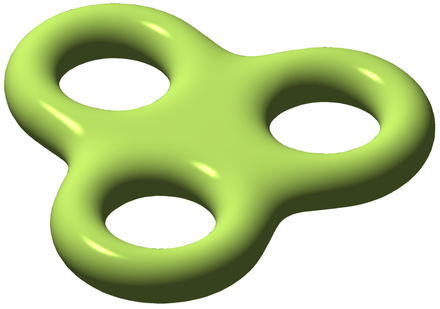
\includegraphics[scale = 1]{RiemannSurface}
**** Riemann Surface of genus 3, from Wikimedia ****

Of course this definition does not apply to curves over fields other than $\CC$, and doesn't relate the genus to the algebra of the curve. However, we can relate the topological genus of a curve directly to its topological Euler characteristic
$
\chi_{top}(C) = 2-2g.
$
By the Hopf index theorem, the topological Euler characteristic is the degree of the tangent sheaf, or equivalently, minus the degree of the cotangent sheaf $\omega_{C}$; that is, $\deg K_{C} = 2g-2$, and thus

$$
g(C) = \frac{\deg(K_C)}{2} + 1.
$$
(This formula serves to define the genus of a smooth projective curve over any field).

Other characterizations of the genus require more machinery to establish. We will give some here, and use  tools from the following section to prove equivalence.

\begin{enumerate}

\item\label{genus 1forms} $g(C)$ is the dimension of the vector space of regular 1-forms (that is, global sections of the
cotangent sheaf) on $C$.

\item The (Zariski) Euler characteristic of the structure sheaf of $C$ is $\chi(\cO_C) = h^0(\cO_C) - h^1(\cO_C)$. Since $h^0(\cO_C) = 1$, 
$$
g(C) = 1 - \chi(\cO_C).
$$

Recall that if $X\subset \PP^{r} = \PP(V)$ is any projective scheme, the \emph{homogeneous coordinate ring} of $X$
is the ring $S/I(X)$ where $S = \Sym V \cong \CC[x_{0}, \dots, x_{r}]$ and $I(V)\subset S$ is the ideal of homogeneous
forms that vanish on $X$.

\item\label{genus Hilbert} Suppose that $C \subset \PP^r = \PP(V)$ is a smooth curve of degree $d$  with homogeneous coordinate ring
$S_C$, then the function $d \mapsto \dim_\CC (S_C)_d$ is equal to a polynomial function $p_C(m)$ for large $d$. We have:
$$
p_C(m) =  dm - g + 1,
$$
so $g(C) = 1 - p_C(0)$. 
\end{enumerate}

\subsection{The Riemann-Roch Theorem}

To prove that these formulas for the genus are correct, we use \trr and Serre duality (sometimes called Kodaira-Serre duality, since Kodaira was responsible for the analytic version.)

\begin{theorem}[Riemann-Roch Theorem]\label{RR}
 If $C$ is a smooth, connected projective curve of genus $g$, and $D$ a divisor of degree $d$ on $C$ then
$$
h^0(D) = d - g + 1 + h^0(K_C - D).
$$
\end{theorem}

For example, if we take $D=0$, this tells us that $h^0(K) = g$, proving the characterization~(\ref{genus 1forms}) above. Also, since $h^0(D) = 0$ for any divisor $D$ of negative degree, the formula gives the dimension of $h^{0}(D)$ when $\deg D$ is large:

\begin{corollary}\label{nonspecial RR}
For any divisor of degree $d \geq 2g-1$, we have
$$
h^0(D) = d - g + 1.
$$
\end{corollary}

Using this, we can apply Proposition~\ref{very ample} to show that all high degree divisors come from embeddings:

\begin{corollary}\label{degree 2g+1 embedding}
Let $D$ be a divisor of degree $d$ on a smooth, connected projective curve of genus $g$. If $d \geq 2g$, the complete linear series $|D|$ is base point free; and if $d \geq 2g+1$ the associated morphism $\phi_D : C \to \PP^{d-g}$ is an embedding, so that
$D$ is the preimage of the intersection of $C$ with a hyperplane in $ \PP^{d-g}$.
\end{corollary}

Since the complement of a hyperplane in projective space is an affine space, we get an affine embedding result too:

\begin{corollary}
 If $C$ is any smooth, connected projective curve and $\emptyset \neq \Gamma \subset C$ a finite subset then $C \setminus \Gamma$ is affine.
\end{corollary}
\begin{proof}
Let $D$ be the divisor defined by $\Gamma$ By Corollary~\ref{degree 2g+1 embedding} a high multiple of $D$ is very ample,
and gives an embedding $\phi: C\to \PP^n$ such that the preimage of the intersection of $C$ with some hyperplane $H$
is a multiple of $D$. It follows that $C\setminus \Gamma$ is embedded in $\PP^n\setminus H$.
\end{proof}


We can  use \TRR in the simple case of Corollary~\ref{nonspecial RR} to determine the Hilbert polynomial of a projective curve. To do this, let $C \subset \PP^r$ be a smooth curve of degree $d$ and genus $g$, and consider the exact sequence of sheaves
$$
0 \rTo \cI_{C/\PP^r}(m) \rTo \cO_{\PP^r}(m) \rTo \cO_C(m) \rTo 0
$$
and the corresponding exact sequence
$$
 H^0(\cO_{\PP^r}(m)) \rTo^{\rho_m} H^0(\cO_C(m)) \rTo H^1(\cI_{C/\PP^r}(m)) \rTo 0.
$$

The \emph{Hilbert function} $h_C$ of $C$  is defined by
$$
h_C(m) = \dim_{\CC} (S_{C})_{m} = \rank(\rho_m).
$$
By Theorem~\ref{Serre vanishing} we have $H^1(\cI_{C/\PP^r}(m)) = 0$ for large $m$, so $h_{C}(m) = h^0(\cO_C(m))$, for large $m$, which, by \trr, equals $md-g+1$, again for large $m$. Thus, the Hilbert polynomial of $C \subset \PP^r$ is $p_C(m) = dm-g+1$, establishing the characterization~(\ref{genus Hilbert}).
 
The Riemann-Roch formula does \emph{not} give us a formula for the dimension $h^0(D)$ when $h^0(K_C - D)>0$; such divisors $D$ are called \emph{special divisors}, or \emph{special divisor classes}. The existence or non-existence of divisors $D$ with given $h^{0}(D)$ and $h^{1}(D)$ often serves to distinguish one curve from another, and will be an important part of our study.
 
 
\begin{fact}
 Classically, the dimension $h^0(K_C-D) = h^1(D)$ was called the \emph{superabundance} of $D$: the idea was that a divisor of degree $d$ had, at a minimum, $d-g+1$ sections and $h^1(D)$ represented the number of ``extra" sections. Even though the introduction of cohomology was still almost a century away, the ranks of cohomology groups $h^1$ had classical names, often involving the term superabundance---a premonition of the Riemann-Roch theorem in general.
\end{fact}
 
\begin{fact}
If $k$ is a field that is not algebraically closed there may be genus 0 curves that are not isomorphic to $\PP^1$. However, they must be``forms'' of $\PP^1$ in the sense that they become isomorphic to $\PP^1$ after extension of scalars to 
the algebraic closure $\overline k$ of $k$. The unique example with $k = \RR$ is the conic $x^2+y^2+z^2 = 0$. Indeed, any form of $\PP^1$ over any field $k$ can all be embedded in $\PP_{k}^2$ (by using the anti-canonical linear system.

The curve $\PP_k^1$ itself may be described as the scheme of left ideals of $k$-vector-space dimension 1 in the ring of
$2\times 2$ matrices over $k$ (such an ideal can be embedded in the matrix ring as a linear combination of the 2 columns in an appropriate sense). More generally, any scheme that is a form of $\PP^1$ over $k$
may be described as the scheme of 1-dimensional left ideals in a central simple ($=$ Azumaya) algebra over $k$---though as a set this scheme has no $k$-rational points unless the algebra is the algebra of $2\times 2$ matrices!
\end{fact}
\subsection{Serre duality}

In general, if $\cF$ and $\cG$ are coherent sheaves on a scheme $X$, we have for every $i$ and $j$ a cup product map
$$
H^i(\cF) \otimes H^j(\cG) \to H^{i+j}(\cF \otimes \cG).
$$

\begin{theorem}[Serre Duality]\label{sd} Let $C$ be a smooth connected projective curves with canonical divisor $K$. We have
 $$
h^1(K) = 1
$$
and the cup product map
$$
H^1(D) \otimes H^0(K-D) \to H^1(K)
$$
is a perfect pairing; that is, it induces a natural isomorphism
$$
H^1(D) = H^0(K-D)^*.
$$
\end{theorem}

\subsection{A partial proof}

Combining \TRR and Serre Duality we get:
\begin{corollary}
 If $C$ is a smooth, connected projective curve and $D$ is a divisor on $C$ then
\end{corollary}
$$
\chi(\sO_C(C)) := h^0(D) - h^1(D) = d-g+1
$$
or in other words, for any invertible sheaf $\cL$ of degree $d$ on $C$,
$$
\chi(\cL) = d-g+1
$$
which is pretty easy to prove. To see this, observe that for any invertible sheaf $\cL$ on $C$ and any point $p \in C$ we have an exact sequence of sheaves
$$
0 \to \cL(-p) \to \cL \to \cL_p \to 0.
$$
It follows that $\chi(\cL(-p)) = \chi(\cL) - 1$, so that Riemann-Roch for $\cL$ is equivalent to Riemann-Roch for $\cL(-p)$. Since any divisor can be obtained from 0 by adding and subtracting points, the Riemann-Roch formula for an arbitrary $\cL$ follows from the special case $\cL = \cO_C$.

\subsection{Clifford's theorem}

\begin{theorem}\label{Clifford}
Let $C$ be a curve of genus $g$ and $\cL$ a line bundle of degree $d \leq 2g-2$. Then
$$
r(\cL) \leq \frac{d}{2}.
$$
Moreover, if  equality holds then we must have either
\begin{enumerate}
\item $d=0$ and $\cL = \cO_C$;
\item $d = 2g-2$ and $\cL = K_C$; or
\item $C$ is hyperelliptic, and $|\cL|$ is a multiple of the $g^1_2$ on $C$.
\end{enumerate}
\end{theorem}

\begin{proof}
The proof of Clifford rests on a very basic construction and observation. 

To start, let $\cD = (\cL,V)$ and $\cE = (\cM, W)$ be two linear series on a curve $C$. By the \emph{sum} $\cD + \cE$ of $\cD$ and $\cE$, we will mean the pair 
$$
\cD + \cE = (\cL \otimes \cM, U) 
$$
where $U \subset H^0(\cL \otimes \cM)$ is the subspace generated by the image of $V \otimes W$, under the multiplication/cup product map $H^0(\cL) \otimes H^0(\cM) \to H^0(\cL \otimes \cM)$---in other words, it's the subspace of the complete linear series $|\cL\otimes \cM|$ spanned by divisors of the form $D+E$, with $D \in \cD$ and $E \in \cE$.

The observation is a simple one:
\begin{lemma}
If $\cD$ and $\cE$ are two nonempty linear series on a curve $C$, then
$$
\dim(\cD + \cE) \geq \dim \cD + \dim \cE.
$$
\end{lemma}
(To see this, we observe that to say $\dim \cD \geq m$ means exactly that we can find a divisor $D \in \cD$ containing any given $m$ points of $C$; since $\cD + \cE$ contains all pairwise sums $D + E$ with $D \in \cD$ and $E \in \cE$, we can certainly find a divisor $F \in cD + \cE$ containing any given $\dim \cD + \dim \cE$ points of $C$.)

Given this lemma, the proof of Clifford follows simply by applying it to the pair $|\cL|$ and $|K_C\otimes \cL^{-1}|$: by Riemann-Roch, we have
$$
r(K_C\otimes \cL^{-1}) = r(\cL) +g - d - 1
$$
and so we deduce that
$$
g = r(K_C) + 1 \geq r(\cL) + r(K_C\otimes \cL^{-1}) + 1 \geq 2r(\cL) +g - d;
$$
hence $r(\cL) \leq d/2$.

Our proof of the second half of Clifford rests on a basic fact about the geometry of hyperplane sections of a curve in projective space (Proposition~\ref{monodromy of hyperplane section}); we'll defer it until we've established that fact.
\end{proof}



\section{The canonical morphism}

Given the central role played by the canonical divisor class, it is natural to look at the geometry of the morphism $\phi_K : C \to \PP^{g-1}$ associated to the complete canonical series $|K|$.  By the Riemann-Roch theorem, 
$h^{0}(K) = g(C)$, so $|K|$ cannot define a non-constant morphism unless $g(C)\geq 2$, and cannot define an embedding unless $g(C)\geq 3$.

\begin{definition}
A curve $C$ of genus $g \geq 2$ is said to be \emph{hyperelliptic} if there exists a morphism $f: C \to \PP^1$ of degree 2. \end{definition}

%equivalently, if there exists a invertible sheaf $\cL$ on $C$ of degree 2 with $h^0(\cL) = 2$.

\begin{proposition}
The canonical morphism $\phi_K : C \to \PP^{g-1}$ is an embedding if and only if $C$ is not hyperelliptic.
\end{proposition}

\begin{proof}
By Corollary~\ref{degree 2g+1 embedding} we have to show that for any pair of points $p, q \in C$ we have
$$
h^0(K_C(-p-q)) = h^0(K_C)-2 = g-2.
$$
Applying \trr we see that this would fail if and only if $h^0(\cO_C(p+q)) \geq 2$ for some $p,q \in C$, and by Lemma~\ref{deg 2 morphism} $|p+q|$ would define a degree 2 morphism to $\PP^{1}$. 
\end{proof}

\begin{lemma}\label{deg 2 morphism}
Let $C$ be a smooth, projective curve of genus $g\geq 2$. Any invertible sheaf of degree 2 on $C$ defines a morphism to $\PP^{1}$. In particular, if $g(C) = 2$ then the canonical series $|K_{C}|$ defines a 2 to 1 morphism to $\PP^{1}$.
\end{lemma}

\begin{proof}
 If this happens,
we claim that $\cO_C(p+q)$ is basepoint free, so that $C$ is hyperelliptic. To finish the proof, by Corollary~\ref{degree 2g+1 embedding} it suffices to show that
 an invertible sheaf $\sL$ of degree 1 on $C$ must have $h^{0}(\sL)\leq 1$.
 
Suppose that $\sigma_{0}, \sigma_{1}$ were two linearly independent sections of $\sL$. Each $\sigma_{i}$ vanishes at a unique point $p_{i}$. If $p_{0}= p_{1}$ then a linear combination of $\sigma_{0}, \sigma_{1}$ would be a section vanishing to order $\geq 2$, which is impossible, so $\sL$ is basepoint free, and defines a degree 1 morphism $C\to \PP^{1}$. Such a morphism must be an isomorphism (because $\PP^{1}$ is normal), contradicting $g(C) \geq 2$.
\end{proof}

\fix{the following argument is only set-theoretic. Admit this or make it precise}
Note that if $C$ is hyperelliptic, the morphism $\phi_K$ factors through the degree 2 morphism $\pi : C \to \PP^1$: if $\{p,q\} \subset C$ is a fiber of this morphism, we have $h^0(\cO_C(p+q)) = 2$ and hence $\phi_K(p) = \phi_K(q)$. The image of the morphism $\phi_K$ is a nondegenerate curve of degree $g-1$ in $\PP^{g-1}$, which we will see is a \emph{rational normal curve}. This observation implies in particular that if $C$ is hyperelliptic of genus $g \geq 2$, then the invertible sheaf $\cL$ of degree 2 with $h^0(\cL) = 2$ is in fact unique.

Among curves with $g \geq 3$ the hyperelliptic curves are very special: in the family of all curves, as we'll see, they comprise a closed subvariety. Also, the behavior of linear series and morphisms on a hyperelliptic curve is very different from that of series on a general curve; when we discuss the geometry of curves of low genus in the Chapter~\ref{}, we will exclude  the hyperelliptic case, and deal with this case in a separate chapter.

For non-hyperelliptic curves, however, the geometry of the canonical morphism, and its image, the canonical curve, are the keys to understanding the curve. We'll see this in detail in many cases in the following chapter; for now, we mention one highly useful result along these lines.

\fix{add here: canonical series on plane curves cut by $|\cO_{\PP^2}(d-3)|$; consequence that no smooth plane curve can be hyperelliptic}

\fix{maybe move initial discussion of hyperelliptic curves from Ch. 6 to a section here}

\fix{maybe add to this chapter: differentials on plane curves $C$, possibly with nodes or more general singularities; adjoint conditions; algorithm for determining the complete linear system associated to a divisor $D$ on $C$}

\subsection{The geometric Riemann-Roch theorem}

Let's state this first in a relatively simple case: let $C$ be a nonhyperelliptic curve, embedded in $\PP^{g-1}$ by its canonical series and let $D = p_1+\dots + p_d$ be a divisor consisting of $d$ distinct points; let $\overline D$ be the span of the points $p_i \in C \subset \PP^{g-1}$. Since the hyperplanes in $\PP^{g-1}$ containing $\{p_1,\dots,p_d\}$ correspond (up to scalars) to sections of $K_C$ vanishing at all the points $p_i$, we see that
$$
h^0(K_C-D) = g - 1 - \dim \overline D.
$$
Plugging this into the Riemann-Roch formula, we arrive at the statement
$$
r(D) = d - 1 - \dim \overline D;
$$
or in other words, \emph{the dimension of the linear series $|D|$ in which the divisor $D$ moves is equal to the number of linear relations on the points $p_i$ on the canonical curve}. Thus, for example, if $D = p_1+p_2+p_3$, we see that $D$ moves in a pencil if and only if the points $p_i$ are collinear.

We can extend this statement to the case of arbitrary effective divisors $D$ (and even hyperelliptic curves) if we define our terms correctly. To do this, suppose $f : C \to \PP^d$ is any morphism, and $D \subset C$ any divisor. We define the \emph{span} of  $f(D)$ to be the intersection
$$
\overline{f(D)} = \bigcap_{H \mid f^{-1}(H)\supset D} H 
$$
of all hyperplanes in $\PP^d$ whose preimage in $C$ contains $D$. 

\begin{theorem}[Geometric Riemann-Roch Theorem]\label{geometric RR}
If $C$ is any curve of genus $g \geq 2$,  $\phi : C \to \PP^{g-1}$ its canonical morphism and $D \subset C$ any effective divisor of degree $d$, then
$$
r(D) = d - 1 - \dim \overline{\phi(D)}.
$$
\end{theorem}
 

\input footer.tex
%header and footer for separate chapter files

\ifx\whole\undefined
\documentclass[12pt, leqno]{book}
\usepackage{graphicx}
\input style-for-curves.sty
\usepackage{hyperref}
\usepackage{showkeys} %This shows the labels.
%\usepackage{SLAG,msribib,local}
%\usepackage{amsmath,amscd,amsthm,amssymb,amsxtra,latexsym,epsfig,epic,graphics}
%\usepackage[matrix,arrow,curve]{xy}
%\usepackage{graphicx}
%\usepackage{diagrams}
%
%%\usepackage{amsrefs}
%%%%%%%%%%%%%%%%%%%%%%%%%%%%%%%%%%%%%%%%%%
%%\textwidth16cm
%%\textheight20cm
%%\topmargin-2cm
%\oddsidemargin.8cm
%\evensidemargin1cm
%
%%%%%%Definitions
%\input preamble.tex
%\input style-for-curves.sty
%\def\TU{{\bf U}}
%\def\AA{{\mathbb A}}
%\def\BB{{\mathbb B}}
%\def\CC{{\mathbb C}}
%\def\QQ{{\mathbb Q}}
%\def\RR{{\mathbb R}}
%\def\facet{{\bf facet}}
%\def\image{{\rm image}}
%\def\cE{{\cal E}}
%\def\cF{{\cal F}}
%\def\cG{{\cal G}}
%\def\cH{{\cal H}}
%\def\cHom{{{\cal H}om}}
%\def\h{{\rm h}}
% \def\bs{{Boij-S\"oderberg{} }}
%
%\makeatletter
%\def\Ddots{\mathinner{\mkern1mu\raise\p@
%\vbox{\kern7\p@\hbox{.}}\mkern2mu
%\raise4\p@\hbox{.}\mkern2mu\raise7\p@\hbox{.}\mkern1mu}}
%\makeatother

%%
%\pagestyle{myheadings}

%\input style-for-curves.tex
%\documentclass{cambridge7A}
%\usepackage{hatcher_revised} 
%\usepackage{3264}
   
\errorcontextlines=1000
%\usepackage{makeidx}
\let\see\relax
\usepackage{makeidx}
\makeindex
% \index{word} in the doc; \index{variety!algebraic} gives variety, algebraic
% PUT a % after each \index{***}

\overfullrule=5pt
\catcode`\@\active
\def@{\mskip1.5mu} %produce a small space in math with an @

\title{Personalities of Curves}
\author{\copyright David Eisenbud and Joe Harris}
%%\includeonly{%
%0-intro,01-ChowRingDogma,02-FirstExamples,03-Grassmannians,04-GeneralGrassmannians
%,05-VectorBundlesAndChernClasses,06-LinesOnHypersurfaces,07-SingularElementsOfLinearSeries,
%08-ParameterSpaces,
%bib
%}

\date{\today}
%%\date{}
%\title{Curves}
%%{\normalsize ***Preliminary Version***}} 
%\author{David Eisenbud and Joe Harris }
%
%\begin{document}

\begin{document}
\maketitle

\pagenumbering{roman}
\setcounter{page}{5}
%\begin{5}
%\end{5}
\pagenumbering{arabic}
\tableofcontents
\fi


\chapter{Curves of genus 0 and 1}\label{genus 0 and 1 chapter}

In this chapter, we'll begin our project of describing curves in projective space with the simplest cases, that of curves of genus 0 and 1. Despite the relative simplicity of these curves, there are many interesting statements to make about the geometry of their embeddings in $\PP^r$, as well as many conjectures and open problems.

One reason for restricting our attention (for now!) to the cases $g=0$ and $1$ is that the divisor class theory is particularly simple in these cases. Specifically, on a curve of genus 0, there is a unique invertible sheaf of given degree $d$; and on a curve of genus 1 all invertible sheaves of given degree $d$ are congruent modulo the automorphism group of the curve. Thus, in regard to the geometry of the associated maps to projective space, all invertible sheaves of given degree $d$ behave in the same way. By contrast, on a curve $C$ of higher genus there are many different divisor classes of given degree, and to describe their various geometries we need to  introduce and describe the space $\Pic^d(C)$ parametrizing these invertible sheaves. We will do that in the following chapter, and then return in Chapter~\ref{genus 2 and 3 chapter} to the geometry of curves of genera 2 and 3 in projective space. 

Our knowledge of the geometry of curves becomes increasingly less complete as the genus increases, and 6, as we shall see, is a natural turning point; we will consider the case of curves of genus $, 5$ and $6$ in Chapter~\ref{genus 4, 5 and 6 chapter}


\section{Curves of genus 0} 


As we saw in more generality in Example~\ref{linear systems on Pr}, there is for each $d \in \ZZ$  a unique invertible sheaf $\cO_{\PP1} (d)$
of degree $d$ on $\PP^1$. To compute $H^0(\cO_{\PP1} (d))$ directly, let $D = z_1 +z_2 +\cdots+z_d$ be a divisor of degree d and suppose that the coordinates are chosen so that none of the $z_i$ are at infinity. The sections of $\cO_{\PP1} (D)$ are the rational functions with poles only at 
the $z_i$. In affine coordinates, identifying the $z_i$ with complex numbers, these can each be written
$$
\frac{g(z)}{(z-z_1)(z-z_2)\cdots(z-z_d)}
$$
with $\deg(g) \leq d$, the condition that infinity is not a pole. We see that these form a vector space of dimension $d+1$.

\fix{the following result is such a good exercise in the correspondence of linear systems and maps and divisors, maybe move it to Ch 2?}


By \trr, any invertible sheaf of degree $d$ on a curve of genus 0, like $\PP^1$, has at least $d+1$ sections. In fact (over $\CC$, or any algebraically
closed field), this characterizes $\PP^1$:

\begin{theorem}\label{characterization of P1}
Let $C$ be a reduced, irreducible projective curve and let $\cL$ be an invertible sheaf of degree $d$ on $C$. If $\h^0(\cL) \geq d+1$ then
$C \cong \PP^1$, so $\cL \cong \cO_{\PP^1}(d)$, and $\h^0(\cL) = d+1$. 
\end{theorem}

\begin{proof}
Let $p_1,\dots p_{d-1}$ be general points of $C$, and set $\cL':=\cL(-p_1-\cdots-p_{d-1})$. From the correspondence between divisors and
invertible sheaves, we see that the degree of $\cL'$ is $1$.
 Since $\cL$ is locally isomorphic to the sheaf of functions on $C$, the condition of vanishing at a point imposes at most 1 linear condition on 
the global sections of $\cL$, and thus $H^0(\cL') \geq 2$, so we may assume from the outset that $d =1$.

The linear system $(\cL, H^0(\cL))$ cannot have any base points, since
otherwise after subtracting one, we would get an invertible sheaf of degree $\leq 0$ with two independent global sections. Again by the correspondence
with divisors, neither of these sections could vanish at any point of $C$, so their ratio would be a non-constant function defined everywhere on $C$,
a contradiction.

Thus we see that the linear system $(\cL, H^0(\cL))$ defines a morphism $\phi: C\to \PP^1$ of degree 1 whose fibers---the divisors defined by
sections of $\cL$ are of degree 1. Thus if $p\in C$ is the preimage of $q\in \PP^1$, the induced map of local rings
$\phi^*:\cO_{\PP^1, q} \to \cO_{C, p}$ is a finite, birational map. Since $\cO_{\PP^1, q}$ is integrally closed, this is an isomorphism. Thus 
$\phi$ is an isomorphism, as required. 
 \end{proof}

Note that we used the algebraic closure of the ground field in choosing points on $C$.


\begin{corollary}
 Every smooth curve $C$ of genus 0 over an algebraically closed field is isomorphic to $\PP^1$.
\end{corollary}

\begin{proof}
 By \trr, any linear system $\cL$ of degree $d$ on $C$ has $h^0\cL \geq d+1$.
\end{proof}

Note that all the above depends fundamentally on the algebraic closure of the ground field: over a non-algebraically closed field, a curve $C$ of genus 0 need not have any points, or any line bundles of odd degree (since the canonical bundle $K_C$ has degree $-2$, there do necessarily exist line bundles of every even degree; thus an arbitrary curve of genus 0 is isomorphic to a conic plane curve). 
The classification of curves of genus 0 over non-algebraically closed fields is a subject that goes back to Gauss.

%\begin{fact}
%The left ideals of the ring of $2\times 2$ matrices 
%over any field can be indexed by the points of $\PP^1$: to the point $(\lambda, \mu)$ we associate the set of matrices 
%$$\biggl\{
%\begin{pmatrix}
% x_{1,1}&x_{1,2}\\
%  x_{2,1}&x_{2,2}
%\end{pmatrix} \mid \lambda  x_{1,1}+ \mu x_{1,2} = 0,\ \lambda  x_{2,1}+ \mu x_{2,2} = 0\biggr\};
%$$
%for example $(0,1)$ corresponds to the set of matrices with 0 in the second column.
%\def\bH{{\mathbb H}}
%The quaternion algebra 
%$$
%\bH := \RR<i,j,k>/(i^2 = j^2 = -1, ij=k = -ji)
%$$
% is a division ring, so it has no non-trivial left ideals, but
%we can still define the scheme of 2-dimensional left ideals to be the subscheme of the Grassmannian
%$G(2,\bH)$ consisting of 2-dimensional subspaces stable under multiplication by $i,j,k$. This subscheme, which can also be identified with the ``pointless'' conic $x^2+y^2+z^2 = 0$ in $\PP^2_\RR$ has no
%$\RR$-rational points, but $\CC\otimes_\RR \bH$ is the ring of $2\times 2$ matrices over $\CC$, so the set of $\CC$-points
%of the scheme of left ideals of $\bH$ may be identified with $\PP^1_\CC$. It turns out that every scheme over a field $k$ that
%becomes $\PP^1$ over the algebraic closure can be constructed as the scheme of left ideals of a 4-dimensional
%Azumaya (that is, central simple) algebra, in this case a (generalized) quaterion algebra, and as a smooth conic in $\PP^2_k$. There is also a cohomological
%description. See for example Serre ****\fix{I think its in Groupes Algebriques et Corps de Classes, but I'm not sure.}.
%\end{fact}


\section{Rational Normal Curves}

Recall from Example~\ref{Veronese definition} that the image of the $d$-th \emph{Veronese map}  $\phi_d: \PP^1 \to \PP(H^0((\cO_{\PP^1}(d)) \cong \PP^d$ is called the \emph{rational normal curve} of degree $d$. Rational normal curves are probably the most ubiquitous curves in projective space; they have many unique properties, and are extremal in many respects. We will accordingly take a few pages and list some of the special properties of rational normal curves.

\subsubsection{Rational normal curves have minimal degree}
The first is a characterization of rational normal curves as having smallest possible degree among irreducible, nondegenerate curves:

\begin{proposition}
If $C$ is a nondegenerate curve in $\PP^d$ then $\deg C \geq d$, with equality if and only if $C$ is a  rational normal curve.
\end{proposition}

\begin{proof}
 By the correspondence between morphisms and linear systems, the invertible sheaf $\cL$ corresponding to the morphism $C \hookrightarrow \PP^d$ has degree $d$ and
 $h^0(\cL) \geq d+1$. The conclusion follows from Theorem~\ref{characterization of P1}.
\end{proof}

We will see more generally that, if $X$ is a non-degenerate variety in $\PP^d$ of dimension $k$, then $\deg(X) \geq d-k+1$; and we will describe the varieties that achieve the minimum in Section~\ref{**}.

\subsubsection{Independence of points on a rational normal curve}

The points on a rational normal curve are ``as independent as possible:"

\begin{proposition}
If $C\subset \PP^d$ is a rational normal curve of degree $d$ and $\Gamma\subset C$ is a subscheme of length $\ell \leq d+1$, then
$\Gamma$ lies on no plane of dimension $<\ell$. In particular, any $m \leq d+1$ distinct points on a rational normal curve $C \subset \PP^d$ are linearly independent.
\end{proposition}

The rational normal curve is the unique curve with this property, as we shall see in Chapter~\ref{InflectionsChapter}. 

\begin{proof}
We can reduce to the case $\ell = d+1$ by adding points to $\Gamma$, so it suffices to do that case, which follows at once from Bezout's Theorem.
\end{proof}

In the case of distinct points it is easy to make a direct argument: In affine coordinates chosen so that none of the points are
at infinity we can identify the points $\lambda_1,\dots,\lambda_{d+1} \in C \cong \PP^1$ with complex numbers, and the statement (for $\ell = d+1$) is tantamount to the nonvanishing of the Vandermonde determinant
$$
\begin{vmatrix}
1 & \lambda_1 & \lambda_1^2 & \dots & \lambda_1^d \\
1 & \lambda_2 & \lambda_2^2 & \dots & \lambda_2^d \\
\vdots & & & & \vdots \\
1 & \lambda_{d+1} & \lambda_{d+1}^2 & \dots & \lambda_{d+1}^d \\
\end{vmatrix}.
$$

\subsubsection{Rational normal curves are projectively normal}


We say that a smooth curve $C \subset \PP^d$ is \emph{projectively normal} if the restriction map
$$
H^0(\cO_{\PP^d}(m)) \; \to \; H^0(\cO_{C}(m)) 
$$
is surjective for every $m$. We'll this property it in many settings, in particular the discussion of \emph{liaison} in Chapter~\ref{**}.
Since every monomial of degree $md$ on $\PP^1$ is a product of $m$ monomials of degree $d$, we see that the rational normal curve is projectively normal. 


\subsubsection{The equations defining a rational normal curve}
It is easy to write down equations that define a rational normal curve. Choosing a basis $s,t$ for the linear forms on $\PP^1$, we can write
$$
\phi_d : (s,t) \mapsto (s^d, s^{d-1}t,\dots t^d)
$$
from which we see that $C$ lies in the zero locus of the homogeneous quadratic polynomial $z_iz_j - z_kz_l$ for every $i+j=k+l$. As a convenient way to package these, we can realize these forms the $2\times 2$ minors of the matrix
$$
M \; = \; \begin{pmatrix}
z_0 & z_1 & \dots & z_{d-1} \\
z_1 & z_2 & \dots & z_d
\end{pmatrix}.
$$
Note that if we substitute $s^it^{(d-i)}$ for $z_i$ and identify $H^0(\cO_{\PP^1}(i)$ with $\CC[s,t]_i$, this becomes the multiplication table
$$
H^0(\cO_{\PP^1}(i)) \times H^0(\cO_{\PP^1}(d-i-1)) \to H^0(\cO_{\PP^1}(d));
$$
we shall see a general version of this in Chapter~\ref{ScrollsChapter}. 

In fact, the minors of this matrix generate the ideal of forms on $\PP^d$ vanishing on $C$. For this result see for example \cite[****]{E}. 
We can immediately prove two slightly weaker results:

First, $C$ is set-theoretically defined by the $2\times 2$ minors of $M$. Explicitly, suppose that $p = (z_0,\dots,z_d) \in \PP^d$ is any point, and all the polynomials $Q_{ijkl}$ above vanish at $p$. If $z_0 = 0$, then from the vanishing of 
$\det \begin{pmatrix}
z_0 & z_1  \\
z_1 & z_2 
\end{pmatrix}$ 
we see that $z_1 = 0$, and similarly we have $z_2 = \dots = z_{d-1}=0$; this the point $p = (0,\dots,0,1)$, which is a point on the rational normal curve. On the other hand, if $z_0 \neq 0$, set $\lambda = z_1/z_0$; we see in turn that $z_2/z_1 = \dots = z_d/z_{d-1} = \lambda$; thus $p = (1, \lambda, \dots,\lambda^d)$, again a point of the rational normal curve.

Second, the ${d\choose 2}$ distinct $2\times 2$ minors of $M$ are linearly independent, as one can see by first factoring out $x_0$ and $x_d$ and noting that the resulting minors generate the square of the maximal ideal in $\CC[x_1,\dots, x_{d-1}]$. Note that
the restriction map
$$
H^0(\cO_{\PP^d}(2)) \; \to \; H^0(\cO_{C}(2)) = H^0(\cO_{\PP^1}(2d))
$$
 is surjective  because every monomial of degree $2d$ on $\PP^1$ is a product of two monomials of degree $d$. Comparing dimensions, we see that the dimension of the kernel---that is, the space of quadratic polynomials on $\PP^d$ vanishing on $C$---has dimension
$$
\binom{d+2}{2} - (2d+1) \; = \; \binom{d}{2}.
$$


In fact, this gives us another characterization of rational normal curves as extremal: rational normal curves lie on more quadrichypersurfaces than any other irreducible, nondegenerate curve in $\PP^d$.

\begin{proposition}
If $C \subset \PP^d$ is any irreducible, nondegenerate curve, then
$$
h^0(\cI_{C/\PP^d}(2)) \leq  \binom{d}{2};
$$
and if equality holds then $C$ is a rational normal curve
\end{proposition}

\begin{proof}
Consider the restriction of the quadrics containing $C$ to a general hyperplane $H \cong \PP^{d-1} \subset \PP^d$, and let $\Gamma = H \cap C$. We have exact sequence:
$$
0 \to \cI_{C/\PP^d}(1) \to \cI_{C/\PP^d}(2) \to \cI_{\Gamma/\PP^{d-1}}(2) \to 0.
$$ 
Since $C$ is nondegenerate, $h^0(\cI_{C/\PP^d}(1)) = 0$, and since $\deg C \geq d$, the hyperplane section $\Gamma$ of $C$ must contain at least $d$ linearly independent points. Since linearly independent points impose independent conditions on quadrics, we have
$$
h^0(\cI_{\Gamma/\PP^{d-1}}(2)) \leq h^0(\cO_{\PP^{d-1}}(2)) - d,
$$
establishing the desired inequality.
\end{proof}

\begin{exercise}
Establish the analogous statement for hypersurfaces of any degree $d$; that is, no irreducible, nondegenerate curve in $\PP^r$ lies on more hypersurfaces of degree $d$ than the rational normal curve.
\end{exercise}

\begin{exercise}
Prove directly  the special case $r=3$: that the twisted cubic is the unique irreducible, nondegenerate space curve lying on three quadrics. (Hint: if $C \subset \PP^3$ is such a curve lying on three quadrics, what must be the intersection of two of the quadrics containing $C$?)
\end{exercise}

\subsubsection{Rational normal curves are projectively homogeneous}

Another important property of rational normal curves $C \subset \PP^d$ is that they are \emph{projectively homogeneous}: the subgroup $G$ of the automorphism group $PGL_{d+1}$ of automorphisms of $\PP^d$ that carries $C$ to itself acts transitively on $C$. More generally,
every $\PP^r$ is a homogeneous variety in the sense that $\Aut \PP^r$ acts transitively. If $\sigma$ is an automorphism then,
 because $\cO_{\PP^r}(d)$ is the unique
invertible sheaf of degree $d$ on $\PP^r$,  we have $\sigma^*\cO_{\PP^r}(d) = \cO_{\PP^r}(d)$ so $\sigma$ induces an automorphism $\phi$ on $H^0(\cO_{\PP^r}(d))$, and an automorphism $\overline \phi$ on the ambient space $\PP H^0(\cO_{\PP^r}(d))$ of the target of the $d$-th Veronese map. If $\alpha$
is a rational function with divisor $D$, then $\phi(\alpha) = \alpha\circ \sigma$ has divisor $\sigma^{-1}(D)$, so $\overline\phi^{-1}$ induces $\sigma$ on $\PP^r$. 

The rational normal curve $C \subset \PP^r$ can also be characterized among irreducible, nondegenerate curves as the unique projectively homogeneous curve in $\PP^r$, as we shall see in Chapter~\ref{InflectionsChapter}.

\begin{exercise}
Let $\PP^1 \hookrightarrow C \subset \PP^3$ be a twisted cubic. Show that the normal bundle $\cN_{C/\PP^3}$ (defined to be the quotient of the restriction $T_{\PP^3}|_C$ to $C$ of the tangent bundle  of $\PP^3$  by the tangent bundle $T_C$) is 
$$
\cN_{C/\PP^3} \cong \cO_{\PP^1}(5) \oplus  \cO_{\PP^1}(5)
$$
\end{exercise}

\begin{exercise}
Let $\PP^1 \hookrightarrow C \subset \PP^d$ be a rational normal curve. Show that the normal bundle $\cN_{C/\PP^d}$  is 
$$
\cN_{C/\PP^d} \cong \bigoplus_{i=1}^{d-1} \cO_{\PP^1}(d+2).
$$
\end{exercise}

\begin{exercise}
In the situation of the preceding problem, the set  of direct summands of $\cN_{C/\PP^d} $ is a projective space $\PP^{d-2}$. How does the  group of automorphisms of $\PP^d$ carrying $C$ to itself act on this $\PP^{d-2}$?

\end{exercise}

\subsection{Other rational curves}

What about other rational curves in projective space? There are many other embeddings of $\PP^1$ in $\PP^r$ other than the rational normal curve, and we'll talk now about some of these.

The first thing to say is that, since any linear series $\cD$ of degree $d$ on $\PP^1$ is a subseries of the complete series $|\cO_{\PP^1}(d)|$, we see that \emph{any rational curve $C \subset \PP^r$ of degree $d$ is a projection of a rational normal curve in $\PP^d$}. Slightly more generally, any map $\phi : \PP^1 \to \PP^r$ of degree $d$ is given as
$$
z \; \mapsto \; (f_0(z), \dots, f_r(z))
$$
for some $(r+1)$-tuple of polynomials $f_\alpha$ of degree $d$ on $\PP^1$, which is to say it is the composition of the embedding $\phi_d : \PP^1 \to \PP^d$ of $\PP^1$ as a rational normal curve with a linear projection $\pi : \PP^d \to \PP^r$. 

Given how easy it is to describe rational curves in projective space in this way, it is in some ways surprising how many open questions there are about such curves. We'll talk more about some of these questions in the following section; for now, we will try to give a sense of what we can say about such curves by considering one of the first and simplest cases: smooth rational curves of degree $4$ in $\PP^3$.

So: let $C \subset \PP^3$ be a smooth, nondegenerate curve of degree 4 and genus 0 in $\PP^3$. To describe the geometry of $C$, the first thing to determine is what surfaces it lies on---that is, what degree polynomials on $\PP^3$ vanish on $C$. 
\fix{what's proven is that $C$ lies on a smooth quadric and the ideal needs at least 3 additional 3-ic generators. State in advance, and maybe do better.}
To start with, we can ask: does $C$ lie on a quadric surface? To answer this, we consider again the restriction map
$$
H^0(\cO_{\PP^3}(2)) \; \to \; H^0(\cO_{C}(2)) = H^0(\cO_{\PP^1}(8)).
$$
Here the vector space on the left---homogeneous quadratic polynomials on $\PP^3$---has dimension 10, while the one on the right, either by Riemann-Roch or by direct examination, has dimension 9. We conclude that \emph{the curve $C$ must lie on at least one quadric surface $Q \subset \PP^3$}.

Since $C$ is irreducible and nondegenerate, it can't lie on a union of planes, so the quadric $Q$ must either be smooth or a cone over a conic curve. We'll see in a moment that the latter case can't occur, so let's assume for now that $Q$ is smooth. 

The natural follow-up question is, what is the class of $C$ in the Picard group of $Q$? We know that $Q \cong \PP^1 \times \PP^1$, with the fibers of the two projections appearing as lines of the two rulings of $Q$. Lines $L$ and $M$ of the two rulings generate the Picard group \cite[***]{H}, so that we must have $C \sim aL + bM$ for some $a, b$ (in other words, in terms of the isomorphism $Q \cong \PP^1 \times \PP^1$, $C$ is the zero locus of a bihomogeneous polynomial of bidegree $(a,b)$), and we ask what $a$ and $b$ are. The choices are limited: since $C$ is a quartic curve, we must have $a+b = 4$. Adjunction \cite[***]{H} tells us which must be the case: the genus formula for curves on $Q$ tells us that the genus of a smooth curve of class $(a,b)$ on $Q$ has genus $(a-1)(b-1)$, whence the class of our curve $C$ must be $(1,3)$ (for a suitable ordering of the two rulings).

It follows in particular that \emph{$Q$ is the unique quadric containing $C$}. One way to see this is that since $C$ has class $(1,3)$ it meets the lines of the first ruling three times; if $Q'$ is any quadric containing $C$, then, it must contain all these lines and hence must equal $Q$. Equivalently, we may consider the exact sequence
$$
0 \to \cI_{C/Q}(2) \to \cO_Q(2)  \to \cO_C(2) \to 0.
$$
If $C$ has class $L+3M$, we have $\cI_{C/Q}(2) = \cO_{Q}(L-M)$. Since this bundle has negative degree on every line of the first ruling, it has no sections; hence the restriction map $H^0(\cO_Q(2))  \to H^0(\cO_C(2))$ is injective and so there are no  quadrics in $\PP^3$ containing $C$ other than $Q$.

We can also describe the rest of the ideal of $C$ similarly. For example, to find the cubic polynomials vanishing on $C$ we consider the restriction map
$$
H^0(\cO_{\PP^3}(3)) \; \to \; H^0(\cO_{C}(3)) = H^0(\cO_{\PP^1}(12)).
$$
The dimensions of these two vector spaces being 20 and 13 respectively, we see that $C$ must lie on at least 7 cubics; four of these are simply products of $Q$ with linear forms, and so we see that $C$ must lie on at least three cubics modulo those containing $Q$. Indeed, these are easy to spot: if $L$ and $L'$ are any two lines of the first ruling, the divisor $C + L + L'$ has class $(3,3)$ on $Q$ and hence is the intersection of $Q$ with a cubic surface. As $L+L'$ varies in a two-dimensional linear series, we get three cubics containing $C$ modulo those containing $Q$. Conversely, any cubic containing $C$ (but not containing $Q$) will intersect $Q$ in the union of $C$ with a curve of type $(2,0)$ on $Q$, which is to say the sum of two lines of the first ruling, so these are all the cubics containing $C$.

\fix{at least state that these are the generators. And state the set-theoretic
intersection problem.}

Finally, we have to show that the quadric containing the curve $C$ cannot be a cone over a conic plane curve. The key question here is whether or not $C$ contains the vertex $p$ of the cone: if not, the same adjunction-based calculation shows that $C$ must have genus 1; while a parity argument (how many times does $C$ meet a line of the ruling of $Q$?) shows that if a curve $C \subset Q$ of even degree contains $p$ it must be singular there.\fix{this is pretty fast, compared to the level in the rest of the Ch. let's fill it in.}


\begin{exercise}
Find all possible Hilbert functions of smooth rational quintic  curves $C \subset \PP^3$. (There are only two, depending on whether or not $C$ lies on a quadric, so this isn't so bad.)
\end{exercise}

\begin{exercise}
Every $g^3_4$ on $\PP^1$ is uniquely expressible as a sum of the $g_1^1$ and a $g^1_3$
\end{exercise}

\begin{exercise}
There is a 1-parameter family of rational quartic curves in $\PP^3$ up to projective equivalence. (Finding the invariants is a nice problem, which we should talk about. This is the cross-ratio of the roots of the quartic in 2 variables corresponding to the projection center.)
\end{exercise}

\subsection{Further problems (open and otherwise) concerning rational curves in projective space}

To begin with, we should remark that this one example of a non-linearly normal rational curve in projective space is misleading in that we can give such a complete description. For general $d$ and $r$, we have no idea what may be the Hilbert function of a rational curve of degree $d$ in $\PP^r$. Indeed, even in the limited case of $r=3$, our knowledge gives out around $d=9$.

We can, however, say some things about a \emph{general} rational curve $C \subset \PP^r$ of given degree $d$. To make sense of this, let $C_0 \subset \PP^d$ be a rational normal curve of degree $d$. As we've said, any rational curve of degree $d$ in $\PP^r$ is the projection $\pi_\Lambda(C_0)$ of $C_0$ from a $(d-r-1)$-plane $\Lambda \subset \PP^d$. If we let $\GG = \GG(d-r-1, d)$ be the Grassmannian of $(d-r-1)$-planes in $\PP^d$, and we let $U \subset \GG$ be the open subset of planes disjoint from the secant variety of $C_0$, we have a family of rational curves in $\PP^r$ parametrized by $U$ and including every smooth rational curve $C \subset \PP^r$ of degree $d$. Thus in particular we can talk about a \emph{general rational curve} of degree $d$ and genus $g$ in $\PP^r$, and ask about its geometry.

This is, in fact, still largely uncharted waters. Consider, for example, one of the most basic questions we might ask: what is the Hilbert function of a general rational curve $C \subset \PP^r$ of degree $d$? As in the example, this is tantamount to looking at the restriction map
$$
\rho_m : H^0(\cO_{\PP^r}(m) \to H^0(\cO_C(m)) = H^0(\cO_{\PP^1}(md)).
$$
Equivalently, we're asking: if $V$ is a general  $(r+1)$-dimensional vector space of homogeneous polynomials of degree $d$, what is the dimension of the space of polynomials spanned by $m$-fold products of polynomials in $V$? We might naively guess that the answer is, ``as large as possible," meaning that the rank of $\rho_m$ is $\binom{m+r}{r}$ when that number is less than $md+1$, and equal to $md+1$ when it is greater---in other words, the map $\rho_m$ is either injective or surjective for each $m$.

This, it turns out, is true, but it is only relatively recently known: the case $g=0$, as here, was done by Ballico in **** (??), and the analogous statement for curves of arbitrary genus, which we will describe in Chapter~\ref{Brill-Noether}, was proved in 2019 by Eric Larson.

\subsubsection{The secant plane conjecture}

Another question we may ask about a curve in projective space is what secant planes it has. To frame the question, let's start with some language: given a smooth curve $C \subset \PP^r$, we say that an $e$-secant $s$-plane to $C$ is an $s$-plane $\Lambda \cong \PP^s \subset \PP^r$ such that the intersection $\Lambda \cap C$ has degree $\geq e$; if we exclude degenerate cases (for example, where $\Lambda \cap C$ fails to span $\Lambda$), this is the same as saying we have a divisor $D \subset C$ of degree $e$ whose span is contained in an $s$-plane.

Do we expect a curve $C \subset \PP^r$ to have any $e$-secant $s$-planes? The set of $s$-planes in $\PP^r$ is parametrized by the Grassmannian $\GG = \GG(s,r)$, which had dimension $(s+1)(r-s)$. Inside $\GG$, the locus of planes that meet $C$ has codimension $r-s-1$ (the locus of planes containing a given point of $C$ has codimension $r-s$); so our naive expectation might be that the locus of $e$-secant $s$-planes would have codimension $e(r-s-1)$ in $\GG$. Thus we would expect a curve $C \subset \PP^r$ to have $e$-secant $s$-planes when 
$$
e \; \leq \; (s+1)\frac{r-s}{r-s-1}.
$$
Is this true of a general rational curve? For most $e$, $r$ and $s$, we don't know!

\section{Curves of genus 1}

%Wonderful subject; refer to somewhere else. Double cover of $\PP^1$, leading to $y^2 - f(x)$. Plane cubic, quartic in $\PP^3$. Cheerful fact:  elliptic quintic is Pfaffian. Cheerful fact: any $g^5_6$ is the product of two $g^2_3$s. Get a $3\times 3$ matrix of linear forms. The image of the matrix and its transpose are $g^2_3$'s. Prove this by going to the Segre embedding $\PP^2\times \PP^2 \subset\PP^8$.

We cannot begin to describe everything that has been said or done with curves of genus 1, or \emph{elliptic curves}\footnote{Technically, an elliptic curve is a smooth curve of genus 1 with a distinguished point, called the \emph{origin}.}. They appeared, in the second half of the 19th century, as key objects in the developing subjects of geometry, number theory and complex analysis, and the literature is correspondingly rich. Though all curves of genus 0 are isomorphic to $\PP^1$ and on a given curve of genus 0 all divisors of a given degree are linearly equivalent, neither of the analogous statements holds true for curves of genus 1. The ways in which 19th century geometers dealt with this fact has shaped much of algebraic geometry.

Specifically, classical geometers observed that there was a one-parameter family of curves of genus 1 up to isomorphism, and that on a given curve of genus 1 there was a one-dimensional family of divisors up to linear equivalence. These were perhaps the earliest examples of \emph{moduli spaces}, and they were ultimately generalized to the moduli space $M_g$ of curves of genus $g$, and the Picard variety $\Pic^d(C)$ parametrizing divisors of degree $d$ on a given curve $C$ up to linear equivalence.

 Here we will focus on the geometric side, and try to describe maps of genus 1 curves to projective space. As a sort of through-line for our discussion, we will try to indicate in each case how the given projective model of a curve $E$ of genus 1 gives rise to the expectation that there is a one-parameter family of curves of genus 1 up to isomorphism. For any $d$, the automorphism group of $E$ acts transitively on the invertible sheaves of degree $d$ on $E$. In other words, if $\phi, \phi' : E \to \PP^r$ are two maps given by complete linear series $|L|$ and $|L'|$ of degree $d$ on $E$, then there exists  automorphisms $\alpha : \PP^r \to \PP^r$ and $\beta : E \to E$ such that $\phi' \circ \beta= \alpha \circ \phi$. In particular, if $\phi$ and $\phi'$ are embeddings---as will be the case when $d \geq 3$---then their images are projectively equivalent. As for the business of parametrizing invertible sheaves on a given curve $C$, we will take that up in the next chapter, and see it applied in the case of curves of genus $g \geq 2$ in Chapter~\ref{genus 2 and 3 chapter}.

\subsection{Double covers of $\PP^1$}

Let $E$ be a smooth projective curve of genus 1. If $L$ is any invertible sheaf of degree 1 on $E$, \trr says that $h^0(L) = 1$, so if we're looking for nonconstant maps to projective space we have to go to degree 2 and higher.

To start with, suppose $L$ is an invertible sheaf of degree 2 on $E$. By \trr, $h^0(L) = 2$ and the linear series $|L|$ is base point free, so we get a map $\phi : E \to \PP^1$ of degree 2. By \trh, the map $\phi$ will have 4 branch points; by the remark above, these four points are determined, up to automorphisms of $\PP^1$ by the curve $E$, and are independent of the choice of $L$.
After composing with an automorphism of $\PP^1$ we can take these four points to be $0, 1, \infty$ and $\lambda$ for some $\lambda \neq 0, 1 \in \CC$. Since there is a unique double cover of $\PP^1$ with given branch divisor (see~\ref{**}) it follows that $E \cong E_\lambda$, where $E_\lambda$ is the curve given by the affine equation
$$
y^2 = x(x-1)(x-\lambda).
$$

When are two curves $E_\lambda$ and $E_{\lambda'}$ isomorphic? By what we've said, this will be the case if and only if there is an automorphism of $\PP^1$ carrying the points $\{0,1,\infty,\lambda\}$ to $\{0,1,\infty,\lambda'\}$, in any order. This will be the case if and only if $\lambda$ and $\lambda'$ belong to the same orbit under the action of the group $G \cong S_3 \subset PGL(3)$ of automorphisms of $\PP^1$ permuting the three points $0, 1$ and $\infty$. Direct computation shows that the orbit of $\lambda$ is
$$
\lambda' \in \{\lambda, \; 1-\lambda, \; \frac{1}{\lambda},\;  \frac{1}{1-\lambda}, \; \frac{\lambda - 1}{\lambda}, \; \frac{\lambda}{\lambda - 1} \}.
$$
Now, the quotient of $\PP^1$ by the action of $G$ is again isomorphic to $\PP^1$ by Luroth's theorem, which means that the field of rational functions on $\PP^1$ invariant under $G$ is again a purely transcendental extension $K(j)$; explicitly, we can take
$$
j \; = \; 256\cdot \frac{\lambda^2 - \lambda + 1}{\lambda^2(\lambda - 1)^2}.
$$
(the factor of 256 is there for arithmetic reasons). In any case, we see explicitly that there is a unique smooth projective curve of genus 1 for each value of $j$; in particular, the family of all such curves is parametrized by a curve.

\subsection{Plane cubics}

Moving from degree 2 to degree 3, let $L$ be an invertible sheaf of degree 3 on $E$. We see from Corollary~\ref{degree 2g+1 embedding} that the sections of $L$ give an embedding of $E$ as a smooth plane cubic curve; conversely, the genus formula tells us that a smooth plane cubic curve indeed has genus 1. 

We won't delve into the geometry of plane cubics, except to point out that once more we can use this representation to argue that the isomorphism classes of elliptic curves form a 1-dimensional family. To see this, observe that the space of homogeneous polynomials of degree 3 in three variables is 10-dimensional, and the space of plane cubic curves is correspondingly parametrized by  $\PP^9$; the locus of smooth curves is a Zariski open subset of this $\PP^9$. On the other hand, by what we've said, two plane cubics are isomorphic iff they are congruent under the group $PGL_3$ of automorphisms of $\PP^2$. Since the group $PGL_3$ has dimension 8, we would expect that the family of such curves up to isomorphism has dimension 1.

\subsection{Quartics in $\PP^3$} 

Again, let $E$ be a smooth projective curve of genus 1, and consider now the embedding of $E$ into $\PP^3$ given by the sections of an invertible sheaf $L$ of degree 4. The first question we might ask is what polynomial equations in $\PP^3$ cut out the image, and as before we will do this by looking at the restriction map
$$
\rho_2 \;  : \; H^0(\cO_{\PP^3}(2)) \; \to \; H^0(\cO_{E}(2)) = H^0(L^2).
$$
The space on the right---the space of homogeneous polynomials of degree 2 in four variables---has dimension 10, while by Riemann-Roch the space $H^0(L^2)$ has dimension 8. It follows that $E$ lies on at least two linearly independent quadrics $Q$ and $Q'$. Since $E$ does not lie in any plane, neither $Q$ nor $Q'$ can be reducible; thus by \bt we see that
$$
E = Q \cap Q'
$$
is the complete intersection of two quadrics in $\PP^3$. Moreover, we also see from the Lasker-Noether ``AF+BG" theorem that the kernel of $\rho_2$ is exactly the span of $Q$ and $Q'$. Thus $E$ determines a point in the Grassmannian $G(2, H^0(\cO_{\PP^3}(2))) = G(2, 10)$ of pencils of quadrics; and by Bertini's Theorem, a Zariski open subset of that Grassmannian correspond to smooth quartic curves of genus 1. We can use this to once more calculate the dimension of the family of curves of genus 1: the Grassmannian $G(2,10)$ has dimension 16, while the group $PGL_4$ of automorphisms of $\PP^3$ has dimension 15, so we may conclude that the family of curves of genus 1 up to isomorphism has dimension 1.


\subsubsection{Projective normality II}
\fix{maybe this should be part of the homological algebra development much later}
Observe that last two cases (cubic and quartic genus 1 curves) are projectively normal; extend this to arbitrary smooth complete intersections.

Exercise: $C \subset Q \subset \PP^3$ of class $(a,b)$ is projectively normal iff $|a-b| \leq 1$.


\input footer.tex




\input header.tex

\chapter{Jacobians}\label{new Jacobians chapter}


An essential construction in studying a curve $C$ is the association to a divisor  of an invertible sheaf---in other words, the map
$$
\big\{ \text{effective divisors of degree $d$ on C}\big\} \rTo^\mu \big\{ \text{invertible sheaves of degree $d$ on C} \big\}.
$$
sending $D$ to $\cO_C(D)$.

A priori, this is a map of sets. But it is a fundamental fact that each set may  be given the structure of an algebraic variety in a natural way, so that the map between them is regular. The geometry of this map governs the geometry of the curve in many ways.
In this chapter we will describe the source and target of $\mu$, and give references to proofs of their properties. 

We start with the effective divisors. Since $C$ is smooth, an effective divisor of degree $d$ on $C$ is the same thing as a subscheme $D \subset C$ of dimension 0 and degree $d$, and thus
the family $C_d$ of effective divisors of degree $d$ on $C$ is a Hilbert scheme; see~\ref{hilbert scheme section}. This Hilbert scheme may be identified with
the $d$-th \emph{symmetric power} $C^(d)$  of $C$, described in Section~\ref{symmetric section}. 

The parametrization of the set of invertible sheaves on $C$ of a given degree $d$ by the variety $\Pic_d(C)$ requires different techniques. We will define it by a universal property in the category of schemes, and exhibit its construction as an analytic variety, actually a complex torus $\Jac(C)$, whose group structure reflects the tensor product of
sheaves in $\Pic_0(C)$.
Historically, the algebraic construction was a major milestone first reached in the work of Andre Weil in the middle of
the 20th century, and was the reshaped by Grothendieck and his school. The interested reader will find a beautiful, detailed account both of the history and the 
modern theory of the scheme of divisors and the Picard scheme in the exposition~\cite{Kleiman-PicardScheme}. We will give
more specific references to this text as we go, and the reader will find extensive references to the original literature there.

As an application of the mere existence of the spaces $C_d$ and $\Pic_d$, we show in Theorem~\ref{g+3 theorem} that a general divisor of degree $g+3$ on any curve of genus $g$ gives rise to an embedding in $\PP^3$ as a curve of degree $g+3$. Similar techniques, in Section~\ref{g+2 section} show that a general divisor of degree $g+2$ on any curve gives a birational morphism to a plane curve of degree $g+2$. Moreover, if the curve is not hyperelliptic then its image in $\PP^2$ has  only nodes
as singularities, while in the hyperelliptic case its only singularity is one ordinary $g$-fold point. 

\section{Symmetric products and the universal divisor}\label{symmetric section}

Let $C$ be a smooth curve. The space of effective divisors on $C$ can be characterized by a universal property. 

\begin{definition}
Let $B$ be any scheme. A \emph{family} of effective divisors of degree $d$ on $C$, parametrized by the scheme $B$, is a Cartier divisor $X\subset B\times C$ whose intersection with fibers $\{b\} \times C \cong C$ over points of $B$ are divisors of degree $d$ on $C$.
\end{definition}

Given this, we have a contravariant functor 
$$
F : (schemes) \to (sets),
$$
defined by taking a scheme $B$ to the set of families of divisors of degree $d$ over $B$; if $\pi : B' \to B$ is any morphism, the induced map $F(B) \to F(B')$ is defined by taking a family $\cD \subset B \times C$ to the preimage of $\cD$ under the map $\pi \times Id : B' \times C \to B \times C$. We say that a scheme $C_d$ is a fine moduli space for divisors of degree $d$ on $C$ if we have an isomorphism of functors
$$
F \cong \Hom_{\rm{Schemes}}( -, C_d).
$$
By Yoneda's Lemma, this is equivalent to the existence of a \emph{universal family} $\cD \subset C_d \times C$, with the property that for any family $X \subset B \times C$ of divisors on $C$ over any scheme $B$, there is a unique map $\phi : B \to C_d$ such that $X = (\phi \times id_{C})^{-1}(\cD)$.

From the universal property it is clear that a fine moduli space for divisors of degree $d$ on $C$ is unique if it exists. Indeed, it does exist, and we'll sketch the construction, using symmetric products. This construction relies on the existence of quotients of schemes by finite groups, and we'll pause here to discuss such quotients.

\subsection{Finite group quotients}

If $G$ is a finite group acting by automorphisms on an affine scheme $X:=\Spec A$ then $X/G$ is by definition $\Spec(A^G)$, the spectrum of the ring $A^G$ of invariant elements of $A$. The following result shows that this definition reflects the desired
geometry: 

\begin{theorem}\label{finite invariant theory}
 The map $\pi: X\to X/G$ induced by the inclusion of rings is finite. If $X$ is a normal variety, then the fibers of $\pi$  are the orbits of $G$.
\end{theorem}
For a proof, see for example \cite[Proposition 13.10]{Eisenbud1995}).  

Since the map $X\to X/G$ is finite, we have $\dim X/G = \dim X$. 

The construction commutes with the passage to $G$-invariant open affine sets, and thus passes to more general schemes---and in particular to projective schemes (Exercise~\ref{quotient of projective})---as well.

When the group $G$ is infinite, the situation becomes much more complex---see Chapter~\ref{ModuliChapter} for some  idea of what can and cannot be done.

For example, if $X$ is any scheme or any quasi-projective variety $X$ we define the \emph{$d$-th symmetric power $X^{(d)}$ of $X$} to be the quotient of the Cartesian product $X^d$ of $d$ copies of $X$ by the action of the group of permutations of the factors. 

%Since an effective divisor of degree $d$ on a curve $C$ is an unordered $d$-tuple of points on $C$, with repetitions allowed, it corresponds to a point in the \emph{$d$th symmetric power} $C^{(d)}$. For this reason we will write the points of $\Cd$ as $d$-tuples.

If $X=\AA^{1}$ then $X^{d} = \AA^{d} = \Spec \CC[x_{1}, \dots, x_{d}]$. The ring of invariants of the symmetric group acting on
$\CC[x_{1}, \dots, x_{d}]$ by permuting the variables is generated by the $d$ elementary symmetric functions, which generate a polynomial subring, and $X^{(d)}$ is isomorphic to $\AA^{d}$. Since the symmetric functions of the roots of a polynomial in one variable are the coefficients of
that polynomial, we may identify $X^{(d)}$ with the affine space of monic polynomials of degree $d$ in $\CC[z]$. (\cite[Exercises 1.6, 13.2-13.4]{Eisenbud1995})

Next consider $X = \PP^1$ and the product $(\PP^1)^d$. Taking the homogeneous coordinates of the
$i$-th copy of $\PP^1$ to be $(s_i,t_i)$, the $d+1 $multilinear symmetric functions of degree $d$,
$$
t_1t_2\cdots t_d,\ s_1t_2\cdots t_d,\ \dots,\ s_1\cdots s_d
$$
are the coefficients of the polynomial
$$
(s_1\lambda + t_1\mu)(s_2\lambda + t_2\mu)\cdots(s_d\lambda + t_d\mu)
$$
defining a general subcheme of $\PP^1$ of degree $d$ and  define
an isomorphism $(\PP^1)^{(d)} \to \PP^d$.
Again, we may think of this map as taking a $d$-tuple of points to the unique-up-to-scalars
homogeneous form of degree $d$ vanishing on it.

We shall see that when $C$ is a smooth curve of higher genus, the global geometry of $C^{(d)}$ is quite nontrivial, but at least
the local geometry is simple:

\begin{proposition}
If $C$ is a smooth curve then each symmetric power $C^{(d)}$ is smooth.
\end{proposition}

\begin{proof}
 The general case follows from the case of $\AA^{1}$ because locally analytically the action of the symmetric group on $C^d$ is the same as for $\AA^1$: If  $\overline p \in X^{(d)}$, then it suffices to
 show that the quotient of an invariant formal neighborhood of the preimage $p_1,\dots, p_s$ of
 $\overline p$ is smooth. After completing the local rings, we get an action of the symmetric group
 $G$ on the product of the completions of $X$ at the $p_i$, and this depends only on the orbit
 structure of $G$ acting on $\{p_1,\dots, p_s\}$. Thus it would be the same for some orbit of
 points on $\AA^1$.
 \end{proof}

By contrast, if $\dim X \geq 2$ then the symmetric powers $X^{(d)}$ are singular for all $d \geq 2$.
See Exercise~\ref{sym2A2} for the case of $(\AA^2)^{(2)}$ and Exercise~\ref{free actions} for a well-behaved case.

It is clear from Theorem~\ref{finite invariant theory} that the points of $C^{(d)}$ are in one-to-one correspondence with the effective divisors of
degree $d$ on $C$, but much more is true:

\begin{theorem}
 If $C$ is a smooth projective curve, then the $d$th symmetric power $C^{(d)}$ of $C$ is the fine moduli space $C_d$ for effective divisors of degree $d$ on $C$.
\end{theorem}
For a proof in the analytic category, see \cite[]{ACGH}; for the algebraic fact, see \cite[Remark 9.3.9]{Kleiman-PicardScheme}.
Henceforward we will write $C_d$ in place of $C^(d)$ for this space.


%Finally we come to the definition of the universal family:
%
%\begin{fact}
% The universal family of degree $d$ divisors on $C$ is the incidence correspondence $\sD\rTo^\alpha \Cd$ where
% $\sD \subset C \times \Cd$ is the incidence correspondence 
%$$
%\sD := \{(x,(x_1,\dots x_d)) \mid x = x_i\hbox{ for some }i\}.
%$$
%and thus the Hilbert scheme of degree $d$ subschemes of $C$ is $\Cd$.
%
%If $X \to C\times B$ is a family of divisors of degree $d$ on $C$ then we may define a set-theoretic map $\phi: B\to \Cd$ by sending $b\in B$ to the
%unordered $d$-tuple of points of the divisor that is the fiber over $b$. This together with the composition $X \to C \rTo^1 C$
%gives us the diagram in the Theorem, and it can be shown that the map $\phi$ is a map of schemes.
%\end{fact}

%\fix{seems a pity not to prove this -- we prove so little in this Chapter Kleiman's reference are to Deligne and the book by Bosch et al on Neron-Severi.}

\section{The Picard varieties}

As with $C_d$, we may define $\Pic_d(C)$ by a universal property. We start by saying what we mean by a family of invertible sheaves on a smooth curve $C$:

\begin{definition}
 For any scheme $B$, a \emph{family of invertible sheaves on $C$ over $B$} is an equivalence class of invertible sheaves $\sL$ on $B\times C$, where two such
 families $\sL$ and $\sL'$are equivalent if they differ by an invertible sheaf pulled back from $B$, that is, if
 $$
 \sL' = \sL \otimes \pi_1^*\cF
 $$
for some invertible sheaf $\cF$ on $B$.
 \end{definition}

If $p \in C$ and $\cF$ is a sheaf on $B$ then $\pi_1^*(\cF)\mid_{B\times p} = \cF$, so we could have eliminated the
equivalence relation at the expense of choosing a point by insisting that the restriction of $\sL$ to $B \times \{p\}$ be trivial.
 
% Thus, given a point $p\in C$, and family of invertible sheaves
% is equivalent to a unique one whose restriction to $\{p\}\times B$ is trivial. 
 

 
We say that $\sL$  is a family of sheaves of degree $d$ if the restriction of $\sL$
 to $C\times \{b\}$ is $d$ for each point $b\in B$. 
 
We define the functor
 $$
 Pic_d : (schemes) \to (sets)
 $$
 by associating to any scheme $B$ the set of invertible sheaves of degree $d$ on $B \times C$, modulo tensoring with pullbacks of invertible sheaves on $B$. Since the tensor product and inverse of an invertible sheaf of degree 0 again has degree 0, 
 $Pic_0$ factors through the category of abelian groups. These functors are representable by schemes:
  
 \begin{fact}\cite[Theorem 9.4.8]{Kleiman-PicardScheme}
 There exists a fine moduli space $\Pic_d(C)$ for invertible sheaves of degree $d$ on $C$; that is, a scheme $\Pic_d(C)$ such that for any scheme $B$ we have a natural bijection between families of invertible sheaves of degree $d$ over $B$, modulo invertible sheaves on $B$, and morphisms $B \to \Pic_d(C)$. The tensor product of invertible sheaves makes $\Pic_0(C)$ an algebraic group, which acts on each $\Pic_d(C)$.
 \end{fact}
 
If $\sL$ is any invertible sheaf of degree $e$ on $C$, we can define a bijection between families of invertible sheaves of degree $d$ over $B$ and families of invertible sheaves of degree $d+e$ over $B$, uniformly for all $B$, by tensoring with the pullback $\pi_2^*\sL$. Thus $\Pic_d(C) \cong \Pic_{d+e}(C)$ (but not canonically, since the isomorphism depends on the choice of $\sL$).
 
 Note also that the variety $\Pic_0(C)$ is a group, with group law given by tensor product of invertible sheaves of degree 0; and for each $d$, $\Pic_d(C)$ is a principal homogeneous space for $\Pic_0(C)$. 
 
 \fix{shouldn't we use the universal properties to produce the map $C_d \to \Pic_d$ at this point?}
 
 Now, on the basis of the characterization of $\Pic_d(C)$ above, it is not at all clear what the geometry of $\Pic_d(C)$ is like: whether it's irreducible, for example, or what its dimension is. In fact, we can get a very good picture of the geometry of $\Pic_d(C)$ from the classical (19th century) construction of the Jacobian, which we'll describe now.
 
% The Jacobian $\Jac(C) = \Pic_0(C)$ is a scheme together with a base point $p\in C$ and an invertible sheaf $\sP$ on $C\times \Jac(C)$ such
% that $\sP|_{\{p\}\times B} = \sO_B$, the trivial sheaf, having the universal property that if $\sM$ is an invertible sheaf on
% $C\times B$, trivial over $\{p\}\times B$, and having degree 0, there is a unique morphism $\phi: B \to \Jac(C)$ such that $\sL = (1\times \phi)^*(\sP).$
% The varieties $\Pic_d(C)$ are all isomorphic to the Jacobian via the map sending an invertible sheaf $\sL$ of degree 0 to $\sL(dp)$, where $p\in C$ is the
%base point.
%
%Just as in the case of the symmetric product, the universal property of the Jacobian and the Picard
%varieties may be expressed as an isomorphism of functors. If $Pic^C_d$ is the functor from Schemes to Sets
%sending a scheme $B$ to the set of families over $B$ of invertible sheaves of degree $d$ on $C$, then
%$$
%Pic^C_d \cong \Hom_{\rm Schemes}(-, \Pic_d(C)).
%$$
%
%The study of the Jacobian began in the 19th century as part of the study of integrals of algebraic equations, described below, 
%and there is an analytic construction that is fairly simple. But the search for an algebraic construction motivated a good deal of the
%algebraic geometry done in the first half of the 20th century. It was finally completed by Weil, and then redone in much greater
%generality by Grothendieck and his school.
%
%\begin{fact}
%If $C$ is a smooth curve then $\Jac(C)$, with its universal bundle, exists as a projective variety, and may be constructed purely algebraically---so that, for example, if the curve $C$ is defined over a given field $K$ then $J(C)$ will be defined over $K$ as well.  
%\end{fact}

\section{Jacobians}

The history leading to the analytic construction of the Jacobian starts from a calculus problem. A goal of the 19th century mathematicians was  to make sense of integrals of algebraic functions. In the early development of calculus, mathematicians figured out how to evaluate explicitly integrals such as
$$
\int_{t_0}^t \frac{dx}{\sqrt{x^2+1}}.
$$
Such integrals can be thought of as path integrals of meromorphic differentials on the Riemann surface associated to the equation $y^2 = x^2+1$. This surface is isomorphic to $\PP^1$, meaning that $x$ and $y$ can be expressed as rational functions of a single variable $z$; making the corresponding change of variables transformed the integral into one of the form
$$
\int_{s_0}^s R(z)dz,
$$
with $R$ a rational function, and such integrals can be evaluated by the technique of partial fractions.

When they tried to extend this to similar-looking integrals, such as
$$
\int_{t_0}^t \frac{dx}{\sqrt{x^3+1}},
$$
which arises when one studies the length of an arc of an ellipse, they were stymied. The reason gradually emerged: the problem is that the Riemann surface associated to the equation $y^2 = x^3+1$ is not $\PP^1$, but rather a curve of genus 1, and so has nontrivial homology group $H_1(C, \ZZ) \cong \ZZ^2$. In particular, if one expresses this ``function'' of $t$  as a path integral, then the value depends on a choice of path; it is defined only modulo a lattice $\ZZ^2 \subset \CC$. This implies that the inverse function is a doubly periodic meromorphic function on $\CC$, and not an elementary function. Many new special functions, such as the Weierstrass $\sP$-function were studied as a result. The name ``elliptic curve'' arose from these considerations.

Once this case was understood, the next step was to extend the theory to path integrals of holomorphic differentials on curves of arbitrary genus. One problem is that the dependence of the integral on the choice of path is much worse; the set of homology classes of paths between two points $p_0, p \in C$ is identified with $H_1(C,\ZZ) \cong \ZZ^{2g}$ rather than $\ZZ^2$, rendering the expression $\int_p^q \omega$ for a given 1-form $\omega$ virtually meaningless.

The solution is to  consider the integrals of \emph{all} holomorphic differentials on $C$ simultaneously---in other words, to consider the expression $\int_p^q$ as a linear function on the space $H^0(K_C)$ of all holomorphic differentials on $C$.

To express the resulting construction in relatively modern terms, let $C$ be a smooth projective curve of genus $g$ over $\CC$, and let $\omega_{C}$ be the sheaf of differential forms on $C$. We will consider $C$ as a complex manifold. Every meromorphic differential form is in fact algebraic
\cite{SerreGAGA}, and we consider $\omega_{C}$ as a sheaf in the analytic topology.

We consider the space $V = H^0(\omega_C)^*$ of linear functions on the space of differentials $H^0(\omega_C)$.  Integration over a closed loop in $C$ defines a linear function on 1-forms, so that we have a map
$$
\iota: \ZZ^{2g} = H_1(C,\ZZ) \; \to \;  H^0(\omega_C)^* \cong H^1(\sO_C) = \CC^{g}.
$$
By Hodge theory, 
$$
H^1(C, \CC) \cong H^1(C, \cO_C) \oplus \overline{H^1(C, \cO_C)}
$$
where the bar denotes complex conjugation $H^1(C, \CC)$, and the map $\iota$ is the composition of 
 the natural inclusion with the projection to the first summand.
 Now
$H_1(C,\CC) = \CC\otimes_\ZZ H_1(C,\ZZ)$, so any basis of $H_1(C,\ZZ)$ maps to a basis of 
 $H^1(C, \CC)$ invariant under conjugation in $H^1(C, \CC)$---See~\cite{Voisin} or~\cite[p. 116]{Griffiths-Harris1978}. 

One can show that the image of $\iota$ is a lattice in $H^0(\omega_C)^*$, and thus the quotient
is a torus of real dimension $2g$. Moreover, the
complex structure on $H^0(\omega_C)^*$ yields a complex analytic structure on the quotient $\CC^{g}/\iota(\ZZ^{2g})$, which is thus a complex torus of  dimension $g$.  

\begin{definition}
 The complex torus $\CC^{g}/\iota(\ZZ^{2g})$ is called the \emph{Jacobian} of $C$.
\end{definition}

The point of this construction is that for any pair of points $p, q \in C$, the expression $\int_q^p$ describes a linear functional on $H^0(\omega_C)$, defined up to functionals obtained by integration over closed loops, and thus a point of $J(C)$. We can think of $p-q$ as a divisor of
degree 0, and the map $p-q \mapsto \int_q^p$ extends to a well defined map $\mu_0$ from divisors of degree 0 to $J(C)$ because
$$
\int_q^p +\int_{q'}^{p'} - (\int_q^{p'} +\int_{q'}^p) 
$$
is the integral around a closed path $q\to p\to q'\to p' \to q$.

Further, if we choose a ``base point''  $p\in C$, we can define the holomorphic map
$$
\mu \; : \; C \; \to \; J(C); \quad q\mapsto \int_{p}^{q}
$$
and more generally maps
$$
\mu_d \; : \; C_d \; \to \; J(C): \quad  \quad (q_1,\dots, q_d) \mapsto \sum_i \int_{p}^{q_i}.
$$

These maps are called the \emph{Abel-Jacobi} maps. When there is no ambiguity about $d$, we will denote all these maps  by $\mu$,  and  
we define $\mu(-D)$ to be $-\mu(D)$. 
The map $\mu$ is a group homomorphism in the sense that if $D, E$ are divisors, then
$\mu (D+E) = \mu(D) + \mu(E)$; this is immediate when the divisors are effective, and 
follows in general because the group of divisors is a free group.

\section{Abel's theorem}
 The connection between the discussion above and the geometry of linear series is made by one of the landmark theorems of the 19th century :

\begin{theorem}[Abel's Theorem]\label{abel}
Two divisors $D, D'$ on $C$ are linearly equivalent if and only if their images under the Abel-Jacobi map are equal, $\mu(D) = \mu(D')$; in other words, the fibers of $\mu_d$ are the complete linear systems of degree $d$ on $C$. Thus $\mu_0$ induces a canonical isomorphism
$\Pic_0(C) \to J(C)$ and after choosing a base point $p$ an isomorphism $\Pic_d(C) \to Jac(C)$, factoring through the isomorphism
$$
\Pic_d(C) \rTo^{-\otimes \sO_C(-dp)} \Pic_0(C) \to J(C).
$$
\end{theorem}


See \cite[Section 2.2]{Griffiths-Harris1978}  for a complete proof of Theorem~\ref{abel}; we will just prove the ``only if" part. This was in fact the only part proved by Abel; the converse, which is substantially more subtle, was proved by Clebsch.

\begin{proof}[Proof of ``only if'']
Suppose that $D$ and $D'$ are linearly equivalent; that is, $\cO_C(D) \cong \cO_C(D')$. Call this invertible sheaf $\cL$, and suppose that $D$ and $D'$ are the zero divisors of sections $\sigma, \sigma' \in H^0(\cL)$.
Taking linear combinations of $\sigma$ and $\sigma'$, we get a pencil $\{D_\lambda\}_{\lambda \in \PP^1}$ of divisors on $C$, with
$$
D_\lambda \; = \; V(\lambda_0\sigma + \lambda_1\sigma'),
$$
and by the universal property of the symmetric product, this corresponds to a regular map $\alpha : \PP^1 \to C^{(d)}$. 

Consider the composition
$$
\phi = \mu \circ \alpha \; : \; \PP^1 \; \to \; J(C).
$$
 If $z$ is any linear functional on $V = H^0(\omega_C)^*$, then, the differential $dz$  on $V$ descends to a global holomorphic 1-form on
 $J(C)$, which is the quotient of $V$ by a discrete lattice. Thus the regular one-forms on $J(C)$ generate the cotangent space to $J(C)$ at every point. But for any 1-form $\omega$ on $J(C)$, the pullback $\phi^*\omega$ is a global holomorphic 1-form on $\PP^1$, and hence identically zero. It follows that the differential $d\phi$ vanishes identically, and hence that $\phi$ is constant, proving that $\mu(D) = \mu(D')$.
\end{proof}

Andre Weil applied Abel's theorem to describe the structure of the Jacobian algebraically:

\begin{corollary}
If $C$ is a smooth curve of genus $g$ then the Abel-Jacobi map $\mu_{g}: C^{(g)} \to J(C)$ is a surjective birational map.
More generally, $\mu_{d}$ is surjective for $d\geq g$ and generically injective for $d\leq g$.
\end{corollary}

\begin{proof}
For $d\leq g = \dim H^{0}(\omega_{C})$,  a divisor $D$ that is the sum of $d$ general points $p_{1}, \dots,  p_{d} \in C$ will impose independent vanishing conditions on the sections of $\omega_{C}$, and thus
$$
h^0(\omega_C(-D)) = g-d,
$$
 Using this, the Riemann-Roch formula gives $h^{0}\cO_{C}(D) = 1$, so the fiber of 
$\mu_{d}$ consists of a single point, proving generic injectivity. In particular when $d= g$, the image of $\mu_{d}$ has
dimension $g$, and since $C^{(g)}$ is compact, the image is closed, so it must be equal to $J(C)$.

Similarly, if $d \geq g$ then $h^0(\omega_C(-D)) = 0$ and hence $r(D) = d-g= \dim C^{(d)} - \dim J(C)$, and it follows that
$\mu_{d}$ is surjective.
\end{proof}

The image of $C_d$ in $J(C)\cong \Pic_d(C)$ can be identified with the set of invertible sheaves 
A priori, these constructions take place in the analytic category; but in fact they are all algebraic:

\begin{fact}
$J(C)$ has the structure of an algebraic group of finite type over $\CC$ (and can be defined over any field where $C$ is defined) and the Abel-Jacobi maps are
maps of algebraic varieties~\cite[]{Kleiman-PicardScheme}.
\end{fact}

\subsubsection{The differential of the Abel-Jacobi map}

Let us consider once more the basic Abel-Jacobi map
$$
\begin{aligned}
\mu_1 : \; &C \to J(C) := H^0(K_C)^*/H_1(C, \ZZ) \\
&q \mapsto \int_p^q 
\end{aligned}
$$
Differentiating under the integral sign, and using the fact that the canonical series $|K_C|$ has no base points, we see \fix{I don't see!} that the differential of this map is nonzero: explicitly, the image of the differential $d\mu_1 : T_q(C) \to T_{\mu_1(q)}J(C) = H^0(K_C)^*$ is the line in $H^0(K_C)^*$ corresponding to the hyperplane $H^0(K_C(-q)) \subset H^0(K_C)$.

If $g(C)>0$ then $p$ cannot be linearly equivalent to $q$ for distinct points $p, q \in C$ so the Abel-Jacobi map $\mu_1$ is one-to-one, and since its differential is nonzero, $\mu_1 : C \to J(C)$ is an embedding. Indeed, since the tangent spaces to $J(C)$ are all identified with $H^0(K_C)^*$, if $Z \subset J(C)$ is a smooth subvariety of dimension $k$ we can define a \emph{Gauss map} $\cG : Z \to G(k, H^0(K_C)^*)$ by sending each point $z \in Z$ to the tangent space $T_{\mu(z)} J(C)$.

\fix{this doesn't make sense: I think it should be
$T_z Z\subset H^0(K_C)^*$ (if that's our notation)}. In particular, the Gauss map applied to the curve $W_1(C) = {\rm Im}(\mu_1)$ is the canonical map! \fix{the notation $W_1$ hasn't been introduced.}


\section{The $g+3$ theorem}

Even after the description of the Picard varieties $\Pic_d(C) \cong J(C)$ in the last section, the Picard varieties may seem like mysterious objects. They are! But even the bare-bones facts---that there exists a  moduli space for invertible sheaves of degree $d$ on $C$, and that this space is irreducible of dimension $g$---suffice to provea non-trivial theorem about curves: 

\begin{theorem}\label{g+3 theorem}
Let $C$ be a smooth projective curve of genus $g$. If $D \in C_{g+3}$ is a general divisor of degree $g+3$ on $C$, then 
$D$ is very ample. In particular, every curve of genus $g$ may be embedded in $\PP^{3}$ as a curve of degree $g+3$.
\end{theorem}

A parallel result, which we will prove in Chapter~\ref{uniformpositionchapter} shows that a general divisor of degree $g+2$ maps the curve birationally to $\PP^2$, onto a curve that either has $\binom{g}{2}$ ordinary nodes and no other singularities unless the curve
is hyperelliptic, in which case it has an ordinary $g$-fold point and no other singularities.

We proved in Theorem~\ref{very ample} that every divisor of degree $\geq 2g+1$ is very ample, and this is sharp: the canonical divisor plus 2 points is not very ample. The difference here is that we are taking a general divisor. Theorem~\ref{g+3 theorem} is also sharp: hyperelliptic curves cannot be embedded in any projective space as curves of any degree less than $g+3$, as we'll see in Chapter~\ref{ScrollsChapter}. 

If we consider only general divisors on \emph{general} curves, we can do still better: the omnibus Brill-Noether theorem (\ref{BN omnibus}) says that``most" curves of genus $g$ can in fact be embedded in $\PP^{3}$ as curves of degree $d = \lceil 3g/4 \rceil + 3$.

\begin{proof}
If $D$ is general of degree $g+3$ then $D$ is nonspecial, so $h^0(\cO_C(D)) = 4$. By Proposition~\ref{very ample} we must show that
for any pair of points $p, q \in C$, we have $h^0(\cO_C(D-p-q)) = 2$.

If, on the contrary, $h^0(\cO_C(D-p-q)) \geq 3$ then by the Riemann-Roch theorem $h^0(\omega_C(-D + p + q)) \geq 1$; fixing a divisor 
$K_{C}\in |\omega_{C}|$, this is the condition that there exists  
an effective divisor $E$ of degree $g-3$ linearly equivalent to a divisor in $|K_C - D + p + q|$. 

Consider the map 
$$
\nu : C^{(g-3)} \times C^{(2)} \; \to \; J(C)
$$
given by
$$
\nu : (E,F) \; \mapsto \; \mu_{2g-2}(K_C) - \mu_{g-3}(E) + \mu_{2}(F), 
$$
where the $+$ and $-$ on the right refer to the group law on $J(C)$. 

By what we have just said and Abel's theorem, a divisor $D$ fails to be very ample only if
$\mu(D) \in {\rm Im}(\nu)$. But the source $C^{(g-3)} \times C^{(2)}$ of $\nu$ has dimension $g-3+2 = g-1$, and so its image in $J(C)$ must be a proper subvariety; since $\mu_{g+3}$ is dominant, the image of a general divisor $D \in C^{(g-3)}$ is a general point of $J(C)$ and thus will not lie in ${\rm Im}(\nu)$. 
\end{proof}

Thus Abel's theorem, which was born out of an effort to evaluate calculus integrals, yields a basic fact in about algebraic curves[


\section{The schemes $W^r_d(C)$}

One of our principal questions, in dealing with a curve $C$, has been to describe the linear series on $C$---the invertible sheaves $\cL$ of a given degree $d$ with an $(r+1)$-dimensional  vector space $V \subset H^0(\cL)$ of sections. We have primarily asked the simple-minded, ``yes-or-no" question, do there exist such linear series or not? But now that we have a parameter space $\Pic_d(C)$ for invertible sheaves of degree $d$, we can substantially refine the question, and ask about the geometry of the locus of such linear series; that is the geometry of
$$
W^r_d(C) := \{ \cL \in \Pic_d(C) \mid h^0(\cL) \geq r+1 \}.
$$
Thus, for example, $W^0_d(C)$ is simply the locus of effective divisor classes, which is to say the image of the natural map $\mu : C_d \to \Pic_d(C)$. (We often omit the ``0" in this case and write this simply as $W_d(C)$.)

Our first step is the observation that \emph{$W^r_d(C)$ is a closed subset of $\Pic_d(C)$}. This follows from upper-semicontinuity of fiber dimension, since we can write
$$
W^r_d(C) = \left\{ \cL \in \Pic_d(C) \mid \dim(\mu^{-1}(\cL)) \geq r \right\}.
$$
Thus $W^r_d(C)$ has the structure of an algebraic variety, and we can talk about its dimension, irreducibility, smoothness or singularity and so on.

We can also introduce the corresponding subvarieties of the symmetric products $C_d$: the preimage $\mu^{-1}(W^r_d) \subset C_d$ parametrizes effective divisors $D$ with $r(D) \geq r$, and is denoted $C^r_d$.

In fact, $W^r_d(C)$ can be given the structure of a scheme representing the functor of families of invertible sheaves with $r+1$ or more sections (that is, the functor that associates to a scheme $B$ the set of invertible sheaves $\cL$ on $B \times C$ such that the pushforward $(\pi_2)_*\cL$ has a locally free subsheaf of rank $r+1$ over every curvilinear subscheme of $B$, as always modulo tensoring with pullbacks of invertible sheaves on $B$). We will later see examples of curves $C$ genus 4 that suggest that the scheme $W^1_3(C)$ is non-reduced, and  curves $C$ of genus 6 suggesting that the scheme $W^1_4(C)$ is non-reduced (in fact isomorphic to $\Spec \CC[\epsilon]/(\epsilon^5)$). \fix{
the claim was that we would see these things; changed to "suggest". OK?} For a definition of the scheme structure, see~\cite[****]{ACGH}. \fix{add ref}

%\section{The $g+2$ theorem}
%
%\fix{We should talk about what to do with this theorem. We could either leave it where it is (with forward references to the elements of the proof coming later); move it to a later chapter; or convert it to a series of exercises somewhere.}
%
%With a little more effort, we can prove an analogue of Theorem~\ref{g+3 theorem} for general linear series of degree $g+2$.
%
%\begin{theorem}
%Let $C$ be any smooth projective curve of genus $g$, and let $D$ be a general divisor of degree $g+2$ on $C$. 
%\begin{enumerate}
%\item If $C$ is non-hyperelliptic, the map $\phi_D : C \to \PP^2$ is birational onto its image $C_0$, and $C_0$ is a plane curve of degree $g+2$ with exactly $\binom{g}{2}$ nodes and no other singularities; and
%\item If $C$ is hyperelliptic, the map $\phi_D : C \to \PP^2$ is birational onto its image $C_0$, and $C_0$ is a plane curve of degree $g+2$ with one ordinary $g$-fold point and no other singularities.
%\end{enumerate}
%\end{theorem}
%
%\begin{proof}
%Let's start by proving that $\phi_D$ is birational onto its image, which is true whether or not $C$ is hyperelliptic. We do this much as in the proof of Theorem~\ref{g+3 theorem}. Since $D$ is general, we know that $h^0(D) = 3$. To say that $\phi_D(p) = \phi_D(q)$ for some pair of points $p, q \in C$, accordingly, means exactly that $h^0(D-p-q) = 2$. This in turn means that $D-p-q = K-E$ for some effective divisor $E$ of degree $g-2$; in other words, to say that $\phi_D(p) = \phi_D(q)$ for some pair of points $p, q \in C$ means that $\mu(D)$ is in the image of the map
%$$
%\nu : C_2 \times C_{g-2} \to \Pic_{g+2}(C)
%$$
%sending $(p+q, E)$ to $K_C - E + p + q$. Now, $\nu$ is a map between projective varieties of the same dimension, so we might expect that it is surjective, and indeed the genus formula tells us that it must be: $\phi_D$ cannot be an embedding. But by the same token, the locus in $\Pic_{g+2}(C)$ over which the fibers of $\nu$ are positive-dimensional must be a proper subvariety; thus for general $D$ we conclude that \emph{there are only finitely many pairs $p, q \in C$ such that $\phi_D(p) = \phi_D(q)$}; in other words, $\phi_D$ is birational onto its image.
%
%Let's now suppose that $C$ is non-hyperelliptic and $D$ is a general divisor of degree $g+2$ on $C$. To prove the theorem in this case, we have to show  three things: that the image $C_0 = \phi_D(C)$ does not have cusps; that it does not have triple points, and that it does not have tacnodes. (The fact that $|D|$ is base point free  will follow from the first of these arguments, as noted below.) We'll take these assertions in turn:
%
%\begin{enumerate}
%
%
%\item Cusps: to say that a point $p \in C$ maps to a cusp of $C_0$ (that is, the differential $d\phi_D$ is zero at $p$) amounts to saying that $h^0(D-2p) \geq 2$; that is, $D-2p$ is a $g^1_g$. But by Riemann-Roch, $W^1_g = K_C - W_{g-2}$; so to say $\phi_D$ has a cusp means that
%$$
%\mu(D) \in 2W_1 + K_C - W_{g-2},
%$$
%and since the locus on the right has dimension at most $g-1$, a general point of $J(C)$ will not lie in it. Note that this subsumes the fact that $|D|$ has no base points.
%
%\item Triple points: to say that $C_0$ has a triple point means that for some divisor $E = p+q+r$ of degree 3, $h^0(D-E) \geq 1$; thus we must have 
%$$
%\mu(D) \in W_3 + W^1_{g-1}
%$$
%Now, to argue that this is not the case, we need to know that $\dim W^1_{g-1} \leq g-4$. Here we have to invoke Marten's theorem, which says that $\dim W^1_{g-1} \leq g-4$ if $C$ is non-hyperelliptic; given this, we conclude that $C_0$ has no triple points.
%
%\item Tacnodes:  To say that a pair of points $p, q \in C$ map to a tacnode of $C_0$ means two things: that $h^0(D-p-q) \geq 2$; and that $h^0(D-2p-2q) \geq 1$. If this is the case, set $E = D - 2p - 2q$;  the condition $h^0(D-2p-2q) \geq 1$ is simply that $E$ is an effective divisor, and by the geometric Riemann-Roch the condition $h^0(D-p-q) \geq 2$ says that in terms of the canonical embedding of $C$, the secant line $\overline{p,q}$ meets the $g-3$-plane $\overline E$ spanned by $E$. Now, not every secant line to $C$ can meet a linear subspace $\Lambda \cong \PP^{g-3}$ of dimension $g-3$---the projection $\pi_\Lambda : C \to \PP^1$ would be constant---so we see that $\mu(D)$ would have to lie on the image of a proper subvariety of $C_{g-2} \times C_2$ under the map 
%$$
%(E, p+q) \mapsto E+2p+2q.
%$$
%By a dimension count it follows that $D$ cannot be a general divisor of degree $g+2$.
%
%\end{enumerate}
%
%Thus, in the non-hyperelliptic case, the image curve $C_0 = \phi_D(C)$ has only nodes as singularities; the fact that there are exactly $\binom{g}{2}$ of them follows from the genus formula.
%
%
%This concludes the proof in the non-hyperelliptic case. The hyperelliptic case is very different, as you might expect from the statement. To analyze this case, suppose that $C$ is hyperelliptic; let $|E|$ be the (unique) $g^1_2$ on $C$. Now, if  $D$ is any divisor of degree $g+2$, the divisor $D - E$ will have degree $g$, and so be effective; thus we can write
%$$
%D = E + p_1 + \dots + p_g
%$$
%for some $g$-tuple of points $p_i$. If the divisor $D$ is general, the points $p_i$ will be general as well, and in particular distinct.
%
%Now, the fact that
%$$
%h^0(D - p_1 - \dots - p_g) = h^0(E) = 2 = h^0(D) - 1
%$$
%says that $\phi_D$ maps all the points $p_i$ to the same point! The image curve $C_0$ thus has a point of multiplicity at least $g$, with at least $g$ branches; by the genus formula, we see that this is an ordinary $g$-fold point of $C_0$ and that $C_0$ can have no other singularities.
%
%\end{proof}

\fix{revised to here 9/16}

\section{Examples in low genus}

\subsection{Genus 1} 

There's not much to say here: if $C$ is a curve of genus 1, the Abel-Jacobi map $\mu : C \to \Pic_1(C)$ is an isomorphism, so that $\Pic_d(C) \cong C$ for all $d$. Equivalently, if we fix any point $q \in C$, we get a map $C \to \Pic_0(C)$ sending $p \in C$ to the invertible sheaf $\cO_C(p-q)$, which is again an isomorphism.

Do note, however, that the isomorphism $C \cong \Pic_0(C)$ does depend on the presence of a point; over non-algebraically closed fields, the Jacobian of a curve $C$ of genus 1 will not in general be isomorphic to $C$. Likewise, the isomorphisms $C \cong \Pic_d(C)$
for $d \neq 1$ do depend on the existence of a divisor of degree $d-1$ on $C$.

\subsection{Genus 2}

First, the map $\mu_1 : C \to J(C)$ embeds the curve $C$ in $J(C)$ (in general, for any curve of genus $g \geq 1$ the map $\mu_1 : C \to J(C)$ is an embedding). 

Secondly, the map $\mu_2 : C^{(2)} \to J(C)$ is an isomorphism except along the locus $\Gamma \subset  C^{(2)} $ of divisors of the unique $g^1_2$ on $C$; in other words, the symmetric square $ C^{(2)} $ of $C$ is the blow-up of $J(C)$ at a point. Exercise~\ref{blow-up of $J(C)$ at a point} justifies this assertion:


\subsection{Genus 3}

Let $C$ be a curve of genus 3. First, we have as before that $\mu_1 : C \to J(C)$ is an embedding. The geometry of the map $\mu_2$, on the other hand, depends on whether  $C$ is hyperelliptic. If it is, $\mu_2$ will collapse the locus in $C_2$ of divisors of the hyperelliptic $g^1_2$ to a point, and $W_2(C)$ will accordingly be singular. If $C$ is not hyperelliptic, by contrast, $\mu_2$ will be an embedding, and $W_2(C)$ smooth.

What about the map $\mu_3$? As we observed in general, for any $g$ the map $\mu_g : C^{(g)} \to J(C)$ is a birational isomorphism. In genus 3, it is the blow-up of $J(C) \cong \Pic_3(C)$ along the locus $W^1_3(C)$. At the same time, we know that
$$
W^1_3(C) = K - W_1(C),
$$
so $W^1_3$ is isomorphic to $C$. Thus $C^{(3)}$ is the blow-up of $J(C)$ along the curve $C$.

\section{Martens' theorem and variants}

The general theorems we have described so far dealing with linear series on a curve $C$, like the Riemann-Roch and Clifford theorems, have to do with the existence or non-existence of linear series on $C$. Now that we've seen how to parametrize the set of linear series on $C$ by the varieties $W^r_d(C)$, we can ask more quantitative questions: for example, what can the dimension of $W^r_d(C)$ be? One basic result, for example, is the following.

\begin{theorem}[Martens' theorem]\cite{Martens}
If $C$ is any smooth projective curve of genus $g$, then for any $d$ and $g$ we have
$$
\dim(W^r_d(C)) \leq d-2r;
$$
moreover, if we have equality for any $r > 0$ and $d < 2g-2$ the curve $C$ must be hyperelliptic.
\end{theorem}

Note that if $C$ is hyperelliptic with $g^1_2 = |D|$, we have
$$
W^r_d(C) \supset W_{d-2r}(C) + \mu(rD).
$$
(In fact, as we'll see in the following chapter, this is an equality.) Since this has dimension $d-2r$, we see that Martens' theorem is sharp. Note also that Clifford's theorem is a special case of Martens' theorem! Finally, note that since
$$
W^r_d(C) = K_C - W^{g-1-d+r}_{2g-2-d}
$$
and
$$
2g-2-d - 2(g-1-d+r) = d-2r,
$$
it will suffice to prove the theorem in case $d \leq g-1$.

Since the fibers of $C^r_d$ over $W^r_d(C)$ have dimension at least $r$, Marten's inequality will follow from the corresponding inequality
$$
\dim C^r_d \; \leq \; d-r.
$$
In this form, it will follow immediately from the geometric form of the Riemann-Roch formula and the elementary

\begin{lemma}[elementary secant plane lemma]\label{elementary secant plane lemma}
Let $C \subset \PP^n$ be a smooth, irreducible and nondegenerate curve. If we denote by $\Sigma \subset C_d$ the locus of effective divisors $D$ of degree $d$ on $C$ with $\dim \overline D \leq d-r-1$, then for any $d \leq n$ and $r > 0$,
$$
\dim \Sigma \leq d-r.
$$
\end{lemma}

\begin{proof}
We will proceed by induction on $d$. To start, let $C^d$ be the Cartesian product and $\alpha : C^d \to C_d$ the quotient map; let $\Phi = \alpha^{-1}(\Sigma)$. Since the fibers of $\pi$ are finite, the lemma is equivalent to the assertion that $\dim \Phi \leq d-r$. Now, consider the projection map $\pi : C^d \to C^{d-r}$ on the first $d-r$ factors. On the one hand, a general $(d-r)$-tuple of points on the curve are linearly independent, so the general fiber of the restriction $\pi_\Phi : \Phi \to C^{d-r}$ is finite. More generally, by the induction hypothesis the locus of $(d-r)$-tuples of points on $C$ that span only a $(d-r-1-s)$-plane has codimension at least $s$ in $C^{d-r}$, and fibers over this locus have dimension $s$, so we conclude that $\dim \Phi \leq d-r$.
\end{proof}

This establishes the Martens inequality, and is completely elementary. To prove the full statement of Martens' theorem---that we have strict inequality in case the curve $C$ is non-hyperelliptic---we need a stronger version of Lemma~\ref{elementary secant plane lemma}. This will require ``borrowing" the general position lemma~\ref{general position lemma} from Chapter~\ref{Brill-Noether}; given this, we can prove the stronger

\begin{lemma}[Strong secant plane lemma]\label{Strong secant plane lemma}
Let $C \subset \PP^n$ be a smooth, irreducible and nondegenerate curve. If we denote by $\Sigma \subset C_d$ the locus of effective divisors $D$ of degree $d$ on $C$ with $\dim \overline D \leq d-r-1$, then for any $d \leq n$ and $r > 0$,
$$
\dim \Sigma \leq d-r-1.
$$
\end{lemma}

\begin{proof}
We set up an incidence correspondence: 
$$
\Gamma := \left\{ (D, H) \in \Sigma \times {\PP^n}^* \mid \overline D \subset H \right\}.
$$
The curve being nondegenerate, the projection map $\Gamma \to  {\PP^n}^*$ is finite. But the fibers of $\Gamma$ over $\Sigma$ have dimension at least $n-d+r$; if we had $\dim \Sigma \geq d-r$, it would follow that $\dim \Gamma \geq n$, and hence that the projection map $\Gamma \to  {\PP^n}^*$ is dominant---contradicting the general position lemma~\ref{general position lemma}.
\end{proof}

There are extensions of Martens' theorem to the case $\dim(W^r_d(C)) < d-2r$ in \cite{Mumford-Prym1} \cite{Keem},
and \cite{Coppens}.

\section{Exercises}

\begin{exercise}
 Let $G$ be a finite group acting on a quasi-projective scheme $X$. Show that there is a finite covering of $X$ by invariant open affine sets. (Hint: consider the sum of the $G$-translates of a very ample divisor.)
\end{exercise}

\begin{exercise}\label{free actions}
We say that a group $G$ acts freely on $X$ if $gx = gy$ only when $g =1$ or $x=y$. Show that
 if $G$ is a finite group acting freely on a smooth affine variety $X$ then the quotient $X/G$ is smooth.
\end{exercise}

\begin{exercise}
 \label{sym2A2} 
 \begin{enumerate}
 \item Let $X = (\AA^{2})^{2}$ and let $G := \ZZ/2$ act on $X$ by permuting the two copies of  $\AA^{2}$; algebraically,
$(\AA^{2})^{2} = \Spec S$, with $S = k[x_{1},x_{2}, y_{1}, y_{2}]$ and the nontrivial element $\sigma\in G$ acts by
$\sigma(x_{i}) = y_{i}$. 
\item Show that $G$ acts freely on the complement of the diagonal, but fixes the diagonal pointwise.
\item Show that the algebra $S^{G}$ has dimension 4 and is generated by the 5 elements
$$ 
f_{1} = x_{1}+y_{1}, f_{2} = x_{2}+y_{2}, g_{1} = x_{1}y_{1}, g_{2} = x_{2}y_{2}, h = x_{1}y_{2}+x_{2}y_{1},
$$
perhaps by appropriately modifying the steps given in \cite[Exercise 1.6]{Eisenbud1995}. 
\item Show that $h^2$ lies in the subring generated by $f_1,\dots, f_4$, and thus $S^{(2)}$ is a hypersurface, singular
along the  codimension 2 subset $f_{1} = f_{2} = 0$, which is the image of the diagonal subset of the 
cartesian product $(\AA^{2})^{2}$.
\end{enumerate}
\end{exercise}

 \begin{exercise}[The universal divisor of degree $d$]\label{universal divisor}
Let $C$ be a smooth projective curve, and $C^{(d)}$ its $d$th symmetric power. Show that the locus
$$
\cD := \{ (D, p) \in C^{(d)} \times C \mid p \in D \}
$$
is a closed subvariety of the product $C^{(d)} \times C$, whose fiber over any point $D \in C^{(d)}$ is the divisor $D \subset C$.

(Hint: consider the $d$th Cartesian product $C^d$, and let
$$
\Delta_i = \{ \left( (x_1,\dots,x_d), x \right) \in C^d \times C \mid x_i = x \}
$$
be the $i$th diagonal. We have a diagram

\begin{diagram}
\bigcup \Delta_i & \rTo & C^d \times C \\
 \dTo & & \dTo \\
 \cD & \rTo & C^{(d)} \times C
\end{diagram}
and since the union $\cup \Delta_i$ is a projective variety, its image $ \cD \subset C^{(d)} \times C$ is closed.)
\end{exercise}


\begin{exercise}
Show that if $r \geq d-g$, then $W^r_d(C) \setminus W^{r+1}_d(C)$ is dense in $W^r_d(C)$ (that is, $W^{r+1}_d(C)$ does not contain any irreducible component of $W^r_d(C)$).
\end{exercise}

\begin{exercise}
Let $C \subset J(C)$ be the image of the Abel-Jacobi map $\mu_1$. Show that the self-intersection of the curve $C$ is 2,
\begin{enumerate}
\item by applying the adjunction formula to $C \subset J(C)$; and
\item by calculating the self-intersection of its preimage $C + p \subset C_2$ and using the geometry of the map $\mu_2$.
\end{enumerate}
\end{exercise}

\begin{exercise}
Consider the map $C \times C \to \Pic_0(C)$ defined by sending $(p, q)\in C \times C$ to the invertible sheaf $\cO_C(p-q)$. What is the degree of this map?
\end{exercise}

\begin{exercise} \label{comparison with geometric RR}
Show more generally that the Abel-Jacobi map $C^{(d)} \to J(C)$ is an immersion on the open subset $C^{(d)} \setminus C^1_d$ \fix{not defined} and that the image of its differential at a point $D \in C^{(d)} \setminus C^1_d$ is  the plane in $\PP^{g-1}$ spanned by the divisor $D$ on the canonical curve (which has the right dimension by the geometric Riemann Roch theorem).
\end{exercise}


\begin{exercise}\label{blow-up of $J(C)$ at a point}
Let $C$ be a curve of genus 2. The canonical map $\phi_K : C \to \PP^1$ expresses $C$ as a 2-sheeted cover of $\PP^1$, and we have correspondingly an involution $\tau : C \to C$ exchanging points in the fibers of $\phi_K$ (equivalently, for any $p \in C$, we have $h^0(K_C(-p)) = 1$; $\tau$ will send $p$ to the unique zero of the unique section $\sigma \in H^0(K_C(-p))$). Let $\Gamma \subset C \times C$ be the graph of $\tau$.
\begin{enumerate}
\item Find the self-intersection of $\Gamma$ in $C \times C$
\item Show the self-intersection of the image of $\Gamma$ in $C_2$ is $-1$.
\end{enumerate}
\end{exercise}

\input footer.tex


%header and footer for separate chapter files

\ifx\whole\undefined
\documentclass[12pt, leqno]{book}
\usepackage{graphicx}
\input style-for-curves.sty
\usepackage{hyperref}
\usepackage{showkeys} %This shows the labels.
%\usepackage{SLAG,msribib,local}
%\usepackage{amsmath,amscd,amsthm,amssymb,amsxtra,latexsym,epsfig,epic,graphics}
%\usepackage[matrix,arrow,curve]{xy}
%\usepackage{graphicx}
%\usepackage{diagrams}
%
%%\usepackage{amsrefs}
%%%%%%%%%%%%%%%%%%%%%%%%%%%%%%%%%%%%%%%%%%
%%\textwidth16cm
%%\textheight20cm
%%\topmargin-2cm
%\oddsidemargin.8cm
%\evensidemargin1cm
%
%%%%%%Definitions
%\input preamble.tex
%\input style-for-curves.sty
%\def\TU{{\bf U}}
%\def\AA{{\mathbb A}}
%\def\BB{{\mathbb B}}
%\def\CC{{\mathbb C}}
%\def\QQ{{\mathbb Q}}
%\def\RR{{\mathbb R}}
%\def\facet{{\bf facet}}
%\def\image{{\rm image}}
%\def\cE{{\cal E}}
%\def\cF{{\cal F}}
%\def\cG{{\cal G}}
%\def\cH{{\cal H}}
%\def\cHom{{{\cal H}om}}
%\def\h{{\rm h}}
% \def\bs{{Boij-S\"oderberg{} }}
%
%\makeatletter
%\def\Ddots{\mathinner{\mkern1mu\raise\p@
%\vbox{\kern7\p@\hbox{.}}\mkern2mu
%\raise4\p@\hbox{.}\mkern2mu\raise7\p@\hbox{.}\mkern1mu}}
%\makeatother

%%
%\pagestyle{myheadings}

%\input style-for-curves.tex
%\documentclass{cambridge7A}
%\usepackage{hatcher_revised} 
%\usepackage{3264}
   
\errorcontextlines=1000
%\usepackage{makeidx}
\let\see\relax
\usepackage{makeidx}
\makeindex
% \index{word} in the doc; \index{variety!algebraic} gives variety, algebraic
% PUT a % after each \index{***}

\overfullrule=5pt
\catcode`\@\active
\def@{\mskip1.5mu} %produce a small space in math with an @

\title{Personalities of Curves}
\author{\copyright David Eisenbud and Joe Harris}
%%\includeonly{%
%0-intro,01-ChowRingDogma,02-FirstExamples,03-Grassmannians,04-GeneralGrassmannians
%,05-VectorBundlesAndChernClasses,06-LinesOnHypersurfaces,07-SingularElementsOfLinearSeries,
%08-ParameterSpaces,
%bib
%}

\date{\today}
%%\date{}
%\title{Curves}
%%{\normalsize ***Preliminary Version***}} 
%\author{David Eisenbud and Joe Harris }
%
%\begin{document}

\begin{document}
\maketitle

\pagenumbering{roman}
\setcounter{page}{5}
%\begin{5}
%\end{5}
\pagenumbering{arabic}
\tableofcontents
\fi


\chapter{Hyperelliptic curves and curves of genus 2 and 3}\label{genus 2 and 3 chapter}

\section{Hyperelliptic Curves}\label{hyperelliptic}
 
We met hyperelliptic curves in Chapter 2, and proved there that, in genus $g \geq 2$, the canonical
map is two to one onto the rational normal curve of degree $g-1$ in $\PP^{g-1}$. We used this to show that every special linear series on a hyperelliptic curve is a sum of a multiple of  the 
unique $g^1_2$ plus base points. We will begin this chapter with an explicit construction of hyperelliptic curves and use it to give a very concrete computation of the canonical series, reproving what we did in Chapter 2. Then we will consider the projective embeddings of curves of genus 2 (which are all hyperelliptic) and genus 3.
 
There will be a further discussion of hyperelliptic curves in Chapter~\ref{ScrollsChapter}, focussing on the algebra and geometry of their projective embeddings. 
  
 \subsection{The equation of a hyperelliptic curve}
 
Recall that a hyperelliptic curve $C$ a curve of genus $\geq 2$ admitting a degree two map $\pi : C \to \PP^1$, and we have seen that such a map is unique. Because the degree is only 2, each point in $\PP^1$ has either two distinct preimages, or only one, a ramification point with ramification index 1, where the map is given in terms of local analytic coordinates on $C$ and $\PP^1$ by $z \mapsto z^2$. In particular, both the ramification divisor and the branch divisor (as defined in Chapter~\ref{linear systems chapter}) are reduced. By the Hurwitz' formula there are exactly $2g+2$ branch points $q_1,\dots,q_{2g+2} \in \PP^1$. These points determine the curve:
 
\begin{theorem}\label{hyperelliptic existence}
There is a unique smooth projective hyperelliptic curve $C$ expressible as a 2-sheeted cover of $\PP^1$ branched over any set of $2g+2$ distinct points.
\end{theorem}

\begin{proof} 
We can easily construct such a curve, postponing for a moment the uniqueness:
If the coordinate of the point $p_i \in \PP^1$ is $\lambda_i$, it is the smooth projective model of the affine curve 
  $$
C^\circ = \big\{ (x,y) \in \AA^2 \; \mid \; y^2 = \prod_{i=1}^{2g+2} (x - \lambda_i) \big\}.
$$ 
Note that we're choosing a coordinate $x$ on $\PP^1$ with the point $x = \infty$ at infinity not among the $q_i$, so that the pre-image of $\infty \in \PP^1$ is two points $r, s \in C$. Concretely, we see that as $x \to \infty$, the ratio $y^2/x^{2g+2} \to 1$, so that 
$$
\lim_{x \to \infty} \; \frac{y}{x^{g+1}} \; = \; \pm 1;
$$
  the two possible values of this limit correspond to the two points $r,s \in C$.
  
  It's worth pointing out that $C$ is \emph{not} simply the closure of the affine curve $C^\circ \subset \AA^2$ in either $\PP^2$ or $\PP^1 \times \PP^1$: as you can see from a direct examination of the equation, each of these closures will be singular at the (unique) point at infinity.
  
   The remainder of the proof of Theorem~\ref{hyperelliptic existence} will be done in a more general situation in Section~\ref{branched covers} below.
  
To give a smooth projective model of the hyperelliptic curve $C$ with given branch divisor, we divide the $2g+2$ branch points  into two sets of $g+1$---say, for example, $q_1,\dots,q_{g+1}$ and $q_{g+2}, \dots, q_{2g+2}$. We can then take $C$ to be the closure in $\PP^1 \times \PP^1$ of the  locus
  $$
  \big\{ (x,y) \in \AA^2 \; \mid \; y^2\prod_{i=1}^{g+1} (x - \lambda_i) = \prod_{i=g+2}^{2g+2} (x - \lambda_i) \big\};
  $$
  in projective coordinates, this is
   $$
  C \; = \; \big\{ (X,Y) \in \PP^1 \times \PP^1 \; \mid \; Y_1^2\prod_{i=1}^{g+1} (X_1 - \lambda_iX_0) = Y_0^2\prod_{i=g+2}^{2g+2} (X_1 - \lambda_iX_0) \big\}.
  $$
To see that $C \subset \PP^1 \times \PP^1$ is smooth we note that it is a curve of bidegree $(2,g+1)$ in $\PP^1 \times \PP^1$, and the formula for the genus of a curve in $\PP^1 \times \PP^1$ derived in Example~\ref{Div of quadric} tells us that such a curve has arithmetic genus $g$, and thus no singular points.

As one consequence of this model, we note the following (which we'll use later in this chapter):

\begin{corollary}\label{relation on ramification points}
If $C$ is a hyperelliptic curve  and $p_1,\dots,p_{2g+2} \in C$ the ramification points of the unique degree 2 map $C \to \PP^1$, then 
$$
p_1+\dots + p_{g+1} \; \sim \; p_{g+2} + \dots + p_{2g+2}.
$$
\end{corollary}
  
 The map $\iota : C \to C$ that exchanges the two points in each reduced fiber of the map $C \to \PP^1$ and fixes the ramification points is algebraic: in terms of the last representation of $C$, it is given by $([X_0,X_1], [Y_0,Y_1]) \mapsto  ([X_0,X_1], [Y_0,-Y_1]) $). The map $\iota$ is called the \emph{hyperelliptic involution} on $C$.

  \subsection{Differentials on a hyperelliptic curve}\label{hyperelliptic differentials}

We can give a pleasantly concrete description of the differentials, and thus the canonical linear system, on a hyperelliptic curve $C$ by working with the affine model $C^\circ = V(f) \subset \AA^2$, where
$$
f(x,y) = y^2 - \prod_{i=1}^{2g+2} (x - \lambda_i).
$$
We will again denote the two points at infinity---that is, the two points of $C \setminus C^\circ$ by $r$ and $s$; for convenience, we'll denote the divisor $r+s$ by $D$. We write $\pi:C \to \PP^1$ for the morphism that, on $C^\circ$, sends $(x,y) \in C$ to $x$.

We can construct a differential form on $C$ by following the proof of Hurwitz' Theorem of Chapter~\ref{linear systems chapter}.
Let $dx$ denote the usual different on $\PP^1$ having a double pole at infinity, and consider $\pi^*dx$ on $C$.  The function $x$ is regular on $C^\circ$, and is a local parameter over points other than the $\lambda_i$; from the local description of the map $\pi$, we see that $\pi^*dx$ is regular on $C^\circ$  with simple zeros at the ramification points $q_i = (\lambda_i, 0)$. Since $dx$ has a double pole at the point at $\infty\in \PP^1$ and $\pi$ is a local isomorphism near $r$ and $s$, the differential $\pi^*dx$ has double poles at the points $r$ and $s$. Thus the canonical
divisor of $C$ is 
$$
(*) \qquad K_C \sim (dx) \sim R - 2D,
$$
where $R$ denotes the ramification divisor, in this case the sum of the ramification points. 

How can we find differentials that are regular everywhere on $C$? If we divide $dx$ by $x^2$ (or any quadratic polynomial in $x$) to kill the poles we  introduce new poles in the finite part $C^\circ$ of $C$. 

Instead, we want to multiply $dx$ by a rational function with zeros at $p$ and $q$, but whose poles occur only at the points where $dx$ has zeroes---that is, the points $q_i$.  A natural choice is the reciprocal of the partial derivative $f_y := \partial f/ \partial y = 2y$, which vanishes at the points $q_i$, and has  a pole of order $g+1$ at each of the points $r$ and $s$ (reason: the involution $y\to -y$ fixes $C^\circ$ and $x$, and exchanges the points $r$ and $s$). In other words, as long as $g \geq 1$, the differential
$$
\omega = \pi^*(\frac{dx}{f_y})
$$
is regular, with divisor
$$
(\omega) = (g-1)r + (g-1)s = (g-1)D.
$$
The remaining regular differentials on $C$ are now easy to find: Since $x$ has only a simple pole
at the two points at infinity we can  multiply $\omega$ by any $x^k$ with $k = 0, 1, \dots, g-1$. Since this gives us $g$ independent differentials, we see that the differentials
$$
\omega, x\omega, \dots, x^{g-1}\omega
$$
  form a basis for $H^0(K_C)$.

With this description of the differentials, we can see clearly why the , canonical map of a hyperelliptic curves is two to one onto a rational normal curve, as proven in Chapter~\ref{2-RR}:
the relations on 
$$
\omega, x\omega, \dots, x^{g-1}\omega
$$
are the relations on $x^i$, and we see that the canonical image is the rational normal curve of degree $g-1$.


\section{Interlude: branched covers with specified branch divisor}\label{branched covers}
   

We will describe here the classification of branched covers $\pi : C \to B$ of a given curve $B$ with specified branch points. To give ourselves a concrete goal, we will address the question: given a curve $B$ and a collection $\Delta = \{p_1,\dots,p_b\} \subset B$ of points in $B$, how many branched covers $\pi : C \to B$ of degree $d$ are there with specified branching over each of the points $p_i$, up to isomorphism over $B$? This is called
the Hurwitz number of the configuration, and its computation in general is the subject of a large and active literature; see for example
\cite{ELSV}.

Our analysis will consist of two steps: first, we will reduce the problem to the classification of topological covering spaces of the complement $U = B \setminus \Delta$; we will then use our knowledge of the fundamental group of $U$ to enumerate such covering spaces.
   
\begin{theorem}
 Let $B$ be a smooth curve, let $\Delta\subset B$ be a finite set of points, and let $U := B\setminus \Delta$.
If $\pi^\circ : V \to U$ is a topological covering space then $V$ may be given the structure of a Riemann surface in a unique way so that the map $\pi^\circ$ is holomorphic; and $V$ may be compactified to a compact Riemann surface $C$ a unique way such that the map $\pi^\circ$ extends to a holomorphic map $\pi : C \to B$.
\end{theorem} 

\begin{proof}
The space $V$ inherits the structure of a complex manifold from $U$ because if $D \subset U$ is any simply connected coordinate chart, then the preimage $({\pi^\circ})^{-1}(D)$ is a disjoint union of $d$ copies of $D$, and we may use them as coordinate charts on $V$. 
   
To compactify $V$ we observe that if $D^* = \{ z \in \CC \mid 0 < |z| < 1 \}$ is a punctured disc, then
the map $D\to D: z \mapsto z^n$ restricts to a connected $n$-fold covering space $D^*\to D^*$. 
Since $\pi_1(D^*) = \ZZ$, any connected covering space $E$ of degree $n$ is homeomorphic to this one
by a homeomorphism inducing the identity on the target of $\pi$.
If we  define a holomorphic structure on $E$ by pulling back the one on $D$, then
this homeomorphism is biholomorphic.

Thus if $D_i$ is a small neighborhood of the point $p_i \in B$ biholomorphic to a disc, then the preimage  in $V$ of the punctured disc $D_i^* := D_i \cap U$ is a disjoint union of punctured discs, and $V$ can then be compactified to a compact Riemann surface in a unique way by completing each one to a full disc.
\end{proof}
   
 The problem of classifying smooth curves $C$ that have a map $\pi : C \to B$ of degree $d$ is thus the problem becomes one of classifying covering spaces of $U$. 
    
 \subsection{Branched covers of $\PP^1$} 

We continue with the notation $U = B\setminus \Delta$, now supposing that $B = \PP^1_\CC$, the Riemann sphere. Again, let $\pi:V\to U$ be a covering space.

Choose a base point $p_0 \in U$, and draw simple, non-intersecting arcs $\gamma_i$ joining $p_0$ to $p_i$ in $U$. If $\Sigma$ is the complement of the union of these arcs in the sphere, then the preimage of $\Sigma$ in $V$ will be the disjoint union of $d$ copies of $\Sigma$, called the \emph{sheets} of the cover; label these $\Sigma_1,\dots,\Sigma_d$.

%\centerline{\includegraphics[height=2in]{"pic41"}}
   
A covering space $V \to U$ of $U$ is determined by its \emph{monodromy}, which is the map
   $$
   \pi_1(U, p_0) \to S_d
   $$
associating to each path  $\beta$ in $U$ from $p_0$ to $p_0$  the permutation of the points of $\pi^{-1}(p_0)$ given by sending a point $q \in \pi^{-1}(p_0)$ to the endpoint of the unique lift of $\beta$ starting at $q$. Let $\beta_i$ be the path starting at $p_0$, going out along the arc $\gamma_i$ until just short of $p_i$, going once around $p_i$ and then going back to $p_0$ along the same path $\gamma_i$, as drawn in the Figure. 

\centerline{ \includegraphics[height=2in]{"pic42"}}

Let $\tau_i$ be the permutation of $\{1,2,\dots,d\}$ corresponding to the path $\beta_i$. The fundamental group of $U$ is the free group of rank $p-1$, generated by the paths $\beta_1,\dots \beta_p$ modulo the relation $\prod_{i=1}^p \beta_i = 1$
which comes from the fact that the sphere minus the part enclosed by the paths $\beta_i$ is 
contractible. In particular, the permutations $\tau_1,\dots,\tau_p$ thus determine the covering space $V$.
 
If we assume that the covering
$\pi : C \to B$ is simply branched, so each $\tau_i$ is a transposition; and if we assume that
$C$, and thus $V$, is connected, then the subgroup $\langle \tau_1, \dots, \tau_b \rangle \subset S_d$ is transitive. If we were to relabel the sheets $\Sigma_\alpha$ according to some permutation $\sigma$, the effect would be to conjugate each $\tau_i$ by $\sigma$. 

Summarizing we have proven:   
   \begin{lemma}\label{branched cover classification}
   Let $p_1,\dots, p_b \in \PP^1$ be any $b$ given points. There is a natural bijection between 
   \begin{enumerate}
   \item the set of  simply branched covers $\pi : C \to \PP^1$ of degree $d$, branched over the points $p_i$, up to isomorphism over $\PP^1$; and
   \item the set of $b$-tuples of transpositions $\tau_1, \dots, \tau_b \in S_d$ such that $\prod \tau_i = id$ and such that $\tau_1, \dots, \tau_b$ generate a transitive subgroup of $S_d$, modulo simultaneous conjugation by $S_d$.
   \end{enumerate}
   \end{lemma}
In the case $d=2$ that is relevant to hyperelliptic curves, we note that there is only one transposition in $S_2$. Thus there is a unique double cover of $\PP^1$ with given branch points $p_1,\dots,p_b$. The product
condition shows again that the number of branch points must be even. . This completes the proof of Theorem~\ref{hyperelliptic existence}.
\end{proof}

We can use the same technique to count the number of 3 to 1 branched covers $C \to \PP^1$ with given simple branch points, using that fact that every odd permutation $\tau \in S_3$ is a transposition. Thus if $b$ is even and  $\tau_1,\dots,\tau_{b-1} \in S_3$ are arbitrary transpositions, then the product 
$\tau_1\cdot \cdots\tau_{b-1}$ is also a
 transposition. It follows that the number of $b$-tuples of transpositions $\tau_1,\dots,\tau_{b} \in S_3$ with $\prod \tau_i$ equal to the identity is $3^{b-1}$. The requirement that the group generated by the $\tau_i$ is transitive eliminates just the three cases where all the $\tau_i$ are equal. The group $S_3$ acts on the set of $b$-tuples of permutations without stabilizing any $b$-tuple, so every cover corresponds to exactly 6 sequences
  $\tau_1,\dots,\tau_b$. In sum, the number of simply branched three-sheeted covers of $\PP^1$ with specified branch points $q_1,\dots,q_b \in \PP^1$ is
$$
\frac{3^{b-1} - 3}{6} \; = \; \frac{3^{b-2} - 1}{2} 
$$


\subsection{More general covers}\label{general covers}

As we indicated, there are natural extensions of this basic theory to covers with arbitrary branching, and to covers of curves of any genus. For the first, suppose that instead of specifying ``simply branched"---meaning that the fiber over any branch point consists of $d-2$ simple points and one double point---we specified that the fiber over a given branch point $q_i$ consisted of $m_1$ simple points, $m_2$ double points, $m_3$ triple points and so on. This amounts to specifying a conjugacy class in $S_d$, and instead of associating to $q_i$ a transposition, we want to specify an element $\tau_i$ of this conjugacy class. Again, the permutations $\tau_i$ have to have product the identity, and to generate a transitive subgroup of $S_d$; and again, they are determined up to simultaneous conjugation by an element of $S_d$.


Similarly, we can enumerate covers of curves $B$ of genus $g>0$ by a modification of the construction above. To do this we must first describe the fundamental group of $B$.
\begin{fact}
  (see \cite[Ch 13]{Munkres}):
Choosing a base point $p \in B$ we can draw $2g$ loops $\alpha_1,\dots,\alpha_{g},\beta_1, \dots, \beta_g$ based at $p$ and disjoint except for $p$ so that the complement $B \setminus \cup \alpha_i$ is a disc $D$ with boundary $\alpha_1, \beta_1, \alpha_1^{-1}, \beta_1^{-1}, \dots, \alpha_g, \beta_g, \alpha_g^{-1}, \beta_g^{-1}$,
and the fundamental group of $B$ is the free group on the classes $\{\alpha_i, \beta_i\}_{i=1,\dots,g}$
modulo the single relation that the product of the commutators is 1:
$$
\prod_{i=1}^g \alpha_i\beta_i\alpha_i^{-1}\beta_i^{-1} = 1.
$$
\end{fact}
We may assume that the base point and branch points of the covering are all within $D$, so if we draw arcs $\gamma_i$ in $D$ joining $p$ to each of the branch points $q_i$, we can associate to a cover a collection of permutations $\sigma_1, \dots, \sigma_b, \mu_1,\dots,\mu_g, \nu_1,\dots,\nu_g$ (with $\sigma_i$ a transposition, if we are assuming simple branching, or of specified conjugacy class in general, and the $\mu_i$ and $\nu_i$ arbitrary). The sequence of these, up to conjugacy, determine the cover, and have to satisfy the relation
$$
\prod_{i=1}^b \sigma_i = \prod_{\alpha=1}^g \; [\mu_\alpha, \nu_\alpha]
$$
and generate a transitive subgroup of $S_d$.


\section{Curves of genus 2}\label{genus 2 section}

Since  curves of genus 2 are hyperelliptic, everything we said above applies to them; in particular, the canonical map $\phi_K : C \to \PP^1$ on a curve of genus 2 is the expression of $C$ as a double cover of $\PP^1$, branched over 6 points in $\PP^1$, which are unique up to automorphisms of $\PP^1$. 

In this section, we'll consider other maps from a hyperelliptic curves $C$ to projective space, starting with maps $C \to \PP^1$.

\subsection{Maps of $C$ to $\PP^1$}\label{genus 2 pencil}

The curve $C$ has a unique degree 2 morphism to $\PP^1$  associated to the canonical system $|K_C|$. But there are many other morphisms to $\PP^1$. For example, there is a 2-parameter
family of maps of degree 3:

 Let $L$ be an invertible sheaf of degree 3 on $C$. Since $3 > 2g-2$, Riemann-Roch tells us immediately that $h^0(L) = 2$, and there are two possibilities:

\begin{enumerate}
\item If the linear system $|L|$ has a base point $p \in C$, then $h^0(L(-p)) = 2$, and hence $L$ must be of the form $L = K_C(p)$. Conversely, if $L = K_C(p)$, then $h^0(L(-p)) = h^0(L)$, which is to say $p$ is a base point of $|L|$. There is a 1-parameter family of such $L$.

\item If $L$ is not of the form $L = K_C(p)$, then $|L|$ does not have a basepoint, and so defines a degree 3 map $\phi_L : C \to \PP^1$.
\end{enumerate}

Since the variety $\Pic^3(C)$ has dimension $g= 2$ the general invertible sheaf of degree 3 is of the second kind, and this gives a 2-parameter family of such maps.

There are plenty of higher-degree maps as well: an invertible sheaf of degree $d \geq 4 = 2g$ is basepoint free
, and gives a map to $\PP^{d-2}$, from which we can project in many ways
to $\PP^1$.

\subsection{Maps of $C$ to $\PP^2$} 
Next consider maps of $C$ of genus 2 to the plane. By theRiemann-Roch theorem, an invertible sheaf $L$ of degree 4 on $C$ will have $h^0(L) = 3$ and is basepoint free by Corollary~\ref{degree 2g+1 embedding} so the linear system $|L|$  gives a morphism $\phi_L : C \to \PP^2$. The invertible sheaf $\sL\otimes \omega_C^{-1}$ is either
$\omega_C$ or nonspecial; in either case, by the Riemann-Roch theorem, it has at least one section, 
so we may write $\sL\otimes \omega_C^{-1} = \sO_C(p+q)$ for some points $p,q$. There are two possibilities:

\begin{enumerate}
\item If $p+q =  K_C$, then $\sL = \omega_C^2$. Since
the elements of $H^0(\omega_C)$ may be written as $\omega, x\omega$, the map
$$
\Sym^2 H^0(\omega_C) \to H^0(\sL).
$$
 is injective, and since both sides are 3-dimensional vector spaces, they are equal. In other words, every divisor $D \sim 2K_C$ is the sum of two divisors $D_1, D_2 \in |K_C|$. We conclude that the map $\phi_L$ is the composition of the canonical map $\phi_K : C \to \PP^1$ with the Veronese embedding $\nu_2 : \PP^1 \to \PP^2$ of $\PP^1$ as a conic in the plane and the map $\phi_L$ is generically 2-to-1 onto the conic.

\item \label{p+q not g12} If $p+q \neq  K_C$  then $h^0(p+q) = 1$, so the pair $p,q$ is unique. Furthermore,
 $h^0(\sL-p) = 2 =  h^0(\sL(-p-q))$ so 
 $H^0(\sL(-p)) = H^0(\sL(-q))$ and $\phi_\sL(p) = \phi_\sL(q)$. 
% However, for any effective divisor $D = r+s$ of degree 2 on $C$  other than $p+q$, we have
%  $h^0(\s(-D)) = 1$, so the map $\phi_\s$ is birational, and the image curve is a plane cubic with one double point.
By the genus formula, the $\delta$ invariant of this point must be 1. By Exercise~\ref{delta=1 characterization}
 this is an ordinary node (if $p\neq q$) or cusp (if $p=q$).

\end{enumerate}

Thus  for $\sL$ in an open subset of $\Pic^4(C)$ the image is a quartic with a node; for a one-dimensional locus in $\Pic^4(C)$, the image is a cubic with a cusp; and for one point in $\Pic^4(C)$ the image is a conic.

\subsection{Embeddings in $\PP^3$}

By Corollary~\ref{degree 2g+1 embedding} any invertible sheaf $L$ of degree 5 is very ample. 
Write $\phi_\sL : C \to \PP^3$ for the map given by the complete linear system $|L|$. Since $\phi_L$ is an embedding, we'll also denote the image $\phi_L(C) \subset \PP^3$ by $C$ and write $\cO_C(1)$ for $L$.

What degree surfaces in $\PP^3$ contain the curve $C$? We start with degree 2, and consider the restriction map
$$
H^0(\cO_{\PP^3}(2)) \to H^0(\cO_C(2)) = H^0(L^2).
$$
The space on the left has dimension 10; by the Riemann-Roch Theorem we have $h^0(L^2) = 2\cdot5 - 2 + 1 = 9$. It follows that $C$ lies on a quadric surface $Q$. Since $C$ a plane or a union of planes, any quadric containing $C$ is irreducible; if there were more than one such, Bezout's Theorem would imply that $\deg(C) \leq 4$. Thus $Q$ is unique.

We might ask at this point: is $Q$ smooth or a quadric cone? The answer depends on the choice of invertible sheaf $L$. 

\begin{proposition}\label{genus 2 embedding}
Let $C \subset \PP^3$ be a smooth curve of degree 5 and genus 2 and $Q \subset \PP^3$ the unique quadric containing $C$. If $L = \cO_C(1) \in \pic^5(C)$, then $Q$ is singular if and only if we have
$$
L \cong K^2(p)
$$
for some point $p \in C$; in this case, the point $p$ is the vertex of $Q$.
\end{proposition}

Note that the variety $\pic^5(C)$ has dimension 2, while the sheaves of the form $K^2(p)$ form a one-dimensional subfamily. Thus in general $Q$ will be smooth; the set of invertible sheaves $L$
for which the quadric is singular is 1-dimensional, and thus of codimension one.

\begin{proof}
First, suppose that the invertible sheaf $L \cong K^2(p)$ for some $p \in C$. Then $L(-p) \cong K^2$, so that the map $\pi : C \to \PP^2$ given by projection from $p$ is the map $\phi_{K^2} : C \to \PP^2$ given by the square of the canonical sheaf. As we've seen, the map $\phi_{K^2}$ is two-to-one onto a conic $E \subset \PP^2$, so that the curve $C$ lies on the cone $Q$ over $E$ with vertex $p$, and this is the unique quadric surface containing $C$.

If $L$ is not of the form $K^2(p)$, then we can write
$$
L = K \otimes M,
$$
where by hypothesis $M$ is not of the form $K(p)$. As we saw in Section~\ref{genus 2 pencil}, this means that the pencil $|M|$ gives a degree 3 map $C \to \PP^1$.

This gives us a way of factoring the map $\phi_L : C \to \PP^3$: we have maps $\phi_K : C \to \PP^1$ of degree 2 and $\phi_M : C \to \PP^1$ of degree 3, and we can compose their product with the Segre embedding $\sigma : \PP^1 \times \PP^1 \to \PP^3$:
\begin{diagram}
& & \PP^1 & & & &\\
& \ruTo^{\phi_K} & & \luTo & & & \\
C & & \rTo^{\phi_K \times \phi_M} & & \PP^1 \times \PP^1 & \rTo^\sigma & \PP^3 \\
& \rdTo^{\phi_M} & & \ldTo & & & \\
& & \PP^1 & & & & \\
\end{diagram}

This description of the map $\phi_L$  shows  that \emph{$C$ is a curve of type $(2,3)$ on a smooth quadric $Q \subset \PP^3$}, completing the proof of Proposition~\ref{genus 2 embedding}.
\end{proof}

To describe a minimal set of generators of the homogeneous ideal $I(C) \subset \CC[x_0, x_1, x_2, x_3]$ in either case, we look at the restriction map
$$
H^0(\cO_{\PP^3}(3)) \to H^0(\cO_C(3)).
$$
Since the dimensions of these spaces are 20 and $15-2+1 = 14$ respectively, we see that  vector space of cubics vanishing on $C$ has dimension at least 6. Only four of these are multiples of the defining equation of $Q$ linear forms on $\PP^3$. It follows that there are at least two cubics vanishing on $C$ that are linearly independent modulo those vanishing on $Q$.

We can identify these cubics geometrically. Suppose first that $Q$ is smooth, so that $C$ is a curve of type $(2,3)$ on $Q$. In that case, if $L \subset Q$ is any line of the first ruling, the sum $C+L$ is the complete intersection of $Q$ with a cubic $S_L$, unique modulo the ideal of $Q$; conversely, if $S$ is any cubic containing $C$ but not containing $S$, the intersection $S \cap Q$ will be the union of $C$ and a line $L$ of the first ruling; thus, mod $I(Q)$, $S = S_L$. A similar argument applies in case $Q$ is a cone, and $L$ is any line of the (unique) ruling of $Q$. In Exercise~\ref{ideal of genus 2 degree 5} you may show that there are no more cubics containing C

\subsection{The dimension of the family of genus 2 curves}

Each of the types of maps that we described from a curve $C$ of genus 2 to projective space suggests
a way to compute the dimension of the family of genus 2 curves, and indeed, as we will explain in Chapter~\ref{ModuliChapter}, there is a moduli space of this dimension.

First, since every curve of genus 2 is uniquely expressible as a double cover of $\PP^1$ branched at six points, modulo the group $PGL_2$ of automorphisms of $\PP^1$. The space of such double covers has dimension 6, and $\dim(PGL_2) = 3$, and since the group acts with finite stabilizers this gives a family of dimension $6-3 = 3$.

Also, each curve  of genus 2 is expressible as a 3-sheeted cover of $\PP^1$ (with eight branch points) in a 2-dimensional family of ways. As we saw in Section~\ref{branched covers}, such a triple cover is determined up to a finite number of choices by its branch divisor, so the space of such triple covers has dimension 8; modulo $PGL_2$ it has dimension 5, and since every curve is expressible as a triple cover in a two-dimensional family of ways, we arrive again at a family of dimension $ 5-2 = 3$.

We've also seen that each curve of genus 2 can be realized as (the normalization of) a plane quartic  with a node in a 2-dimensional family of ways. The space of plane quartics has dimension 14; the family of those with a node has codimension one (Section~\ref{local severi geometry}) and hence dimension 13. It is a fact that the automorphism group of any curve of genus $\geq 2$ is finite, and since  the automorphism group $PGL_3$ of $\PP^2$ has dimension 8, this suggests that that the family of nodal plane quartics modulo $PGL_3$ has dimension 5, and since every curve of genus 2 corresponds to a 2-parameter family of such curves, this again suggests a family of dimension $ 5-2=3$.

Finally, a curve of genus 2 may be realized as a quintic curve in $\PP^3$ in a two-parameter family of ways. To count the dimension of the family of such curves, note that each one lies on a unique quadric $Q$, and is of type $(2,3)$ on $Q$. Thus to specify such a curve we have to specify $Q$ (9 parameters) and then a bihomogeneous polynomial of bidegree $(2,3)$ on $Q \cong \PP^1 \times \PP^1$ up to scalars; these have $3\cdot 4 - 1 = 11$ parameters. Thus there is a 20-dimensional family of such divisors; modulo the automorphism group $PGL_4$ of $\PP^3$, this is a 5-dimensional family. Again, every abstract curve $C$ of genus 2 corresponds to a 2-parameter family of these curves modulo $PGL_4$, so once more this suggests a family of dimension $ 5 - 2 = 3$.

\section{Curves of genus 3}

Let $C$ be a smooth projective curve of genus 3. Since we have already discussed hyperelliptic curves, 
we will assume  that $C$ is nonhyperellitic. By  Theorem~\ref{canonical series is very ample}, the canonical map $\phi_K : C \to \PP^2$ embeds $C$ as a smooth plane quartic curve. Conversely, by Proposition~\ref{Adjunction Formula} any smooth plane curve of degree 4 has genus 3 and is embedded by the complete canonical series. 

Again, the automorphism group of a curve of genus 3 is finite. Since the space of quartics is 14-dimensional, and $\dim PGL(3) = 8$, this suggests that
there is a 6-dimensional family of curves of genus 3, and in Chapter~\ref{ModuliChapter}
we will see that there is indeed a 6-dimensional moduli space.

\subsection{Other representations of a curve of genus 3}
Since we have assumed that $C$ is not hyperelliptic there is no degree 2 cover of $\PP^1$. On the other hand, there are degree 3 covers: if $L \in \pic^3(C)$ is an invertible sheaf of degree 3 then, by the Riemann-Roch Theorem, we have
$$
h^0(L) = 
\begin{cases}
2, &\text{if $L \cong K-p$ for some point $p \in C$; and} \\
1 &\text{otherwise.}
\end{cases}
$$
There is thus a 1-dimensional family of representations of $C$ as a 3-sheeted cover of $\PP^1$. These are  visible directly from the canonical model: a degree 3 map $\phi_{K-p} : C \to \PP^1$ is the composition of the canonical embedding $\phi_K : C \to \PP^2$ with a projection from $p$. 

There are other representations of $C$ as the normalization of a plane curve. By the Riemann-Roch Theorem, $C$ has no $g^2_3$, and the canonical system is the only $g^2_4$, but there are plenty of models as plane quintic curves: by Proposition~\ref{very ample}, if $L$ is any invertible sheaf of degree 5, the linear system $|L|$ will be a basepoint free $g^2_5$ as long as $L$ is not of the form $K+p$, so that $\phi_L$ maps $C$ birationally onto a plane quintic curve $C_0 \subset \PP^2$. These can also be described geometrically in terms of the canonical model: any such invertible sheaf $L$ is of the form $2K-p-q-r$ for some trio of  points $p, q, r \in C$ that are not colinear in the canonical model, and we see  that $C_0$ is obtained from the canonical model of $C$ by applying a Cremona transform with respect to the points $p, q$ and $r$, that is, by applying the birational transformation
of the plane defined by the linear series of conics through $p,q,r$.

Since curves of genus 3 cannot be embedded in the plane, the lowest possible degree of an embedding is 6. Proposition~\ref{very ample} implies that a divisor $D$ of degree 6 is very ample if and only if it is not of the form $K+p+q$ for any $p, q \in C$ and since the family of invertible sheaves on $C$ has dimension 3,  we see that a general invertible sheaf of degree 6 is very ample (indeed, this is a simple case of Theorem~\ref{g+3 theorem}).  

If $C\subset \PP^3$ is a curve of genus 3 embedded as a curve of degree 6, then $C$ cannot lie on a singular quadric since by Example~\ref{Div of quadric} it would
have to be a complete intersection of the quadric with cubic, and then such a curve has genus 4. If $C$ lies on a smooth quadric
in class $(a,b)$ then $a$ or $b$ would be 2, so $C$ would be hyperelliptic, and conversely any curve in class $(2,4)$ 
is a hyperelliptic curve of genus 3, degree 6. 

Thus if $C$ is not hyperelliptic, then $C$ does not lie on a quadric surface. We have $h^0(\sO_{\PP^3}(3)) = 20$ while, by the Riemann-Roch formula, $h^0(\sO_C(3)) = 18-3+1= 16$, so $C$ lies on (at least) 4 cubics. Each of these cubics must be irreducible, so any two of them
intersect in a curve of degree 9 containing $C$ and another component or components $D$ of degree totaling 3. By Bertini's theorem
if we choose two \emph{general} cubics containing $C$, then each of the components of $D$ will be smooth. We shall see in Theorem~\ref{liaison genus formula} that the arithmetic genus of $D$ must be 0; thus $D$ must be a twisted cubic curve. The ideal of the twisted cubic is generated by the $2\times 2$ minors of a matrix of the form
$$
\begin{pmatrix}
 \ell_0& \ell_1&\ell_2\\
 \ell_1& \ell_2&\ell_3\\
\end{pmatrix}
$$
where the $\ell_i$ are linear forms,
and it follows that the two cubics can be written as the two $3\times 3$ minors involving the first two rows of  a matrix of the form
$$
\begin{pmatrix}
 \ell_0& \ell_1&\ell_2\\
 \ell_1& \ell_2&\ell_3\\
\ell_4& \ell_5&\ell_6\\
 \ell_7& \ell_8&\ell_9\\
\end{pmatrix}
$$
where $\ell_4,\dots,\ell_9$ are linear forms as well.
We shall see in Chapter~\ref{SyzygiesChapter}, as an application of the Hilbert-Burch theorem, that the ideal of $C$ is in fact generated by the 4 $3\times 3$ minors of this matrix, whose columns generate
the syzygies of the ideal of the curve.


\section{Theta characteristics}

In this section we sketch the algebraic theory of theta-characteristics, starting with the case of curves of genus 3.

Suppose that $C \subset \PP^2$ is a smooth plane curve. A \emph{bitangent} to $C$ is a line $L \subset \PP^2$ that is either tangent to $C$ at two distinct points, or has contact of order $\geq 4$ with $C$ at a point. Alternatively, we can say that a bitangent  corresponds to an effective divisor of degree 2 on $C$ such that $2D$ is contained in the intersection of $C$ with a line $L \subset \PP^2$.

A naive dimension count suggests that a smooth plane curve should have a finite number of bitangents (it's one condition on a line $L \in {\PP^2}^*$ to be tangent to $C$, so it should be two conditions for it to be bitangent). Indeed, this is the case; by Bezout's Theorem a conic or cubic curve cannot have any bitangents, but as we will show in Section~\ref{plane curve pluecker} every smooth curve of degree $d \geq 4$ has 
$$
12\binom{d+1}{4} - 4d(d-2),
$$
counted with appropriate multiplicities (for example, a line tangent to $C$ at 3 points  counts as three bitangents). Accordingly, a smooth plane quartic has 28 bitangents.

The bitangents to a plane quartic $C$ have a special significance: since $4 = 2 \times 2$, if $D = p+q$ is a bitangent, then the divisor $2D$ comprises the complete intersection of $C$ with a line; in other words, we have a linear equivalence
$$
2D \sim K_C
$$
or equivalently the invertible sheaf $\cO_C(D)$ is a square root of the canonical sheaf of $C$. Because of their appearance in the theory of theta functions, Riemann named the square roots of the canonical sheaf theta-characteristics.

How many such square roots are there? If $\cL$ and $\cM$ are invertible sheaves with $\cL^2 = \cM^2 = K$, then $\cL$ and $\cM$ differ by an invertible sheaf of order 2; that is,
$$
\cM = \cL \otimes \cF, \quad \text{where} \quad \cF \otimes \cF \sim \cO_C.
$$
In other words, $\cF$ is an invertible sheaf of degree 0 and, having fixed $\sL$,  the other sheaf, $\cM$, corresponds to a point of order 2 in the Picard group $\Pic_0(C)$. Since we've seen that $\Pic_0(C) = \Jac(C)$ is a complex torus of dimension g = 3---the quotient of $\CC^3$ by a lattice $\Lambda \cong \ZZ^6$---we see that there are $2^6 = 64$ such invertible sheaves, and thus, given that there is some invertible sheaf $\cL$ satisfying $\cL^2 \cong K_C$, there are exactly $64 = 2^{2g}$ of them.

  
The reader will have noticed that the number 64 of theta-characteristics does not agree with the number 28 of bitangents. The reason is easy to see: bitangents correspond to \emph{effective} divisors $D$ with $2D \sim K$, while a theta characteristic $\cL$ may have $h^0(\cL) = 0$, that is, may not correspond to an effective divisor. 
This situation also occurs in other genera. 
What can we say about the dimensions $h^0(\cL)$ of the space of sections of the theta-characteristics on $C$?
 
 There is a beautiful partial answer to this question, which can be deduced from a remarkable fact: the dimension $h^0(\cL)$ of the space of sections of a theta characteristic mod 2 is invariant in families.
We will now
sketch the necessary results; see~\cite{MumfordPaper} and~\cite{JHPaper} for a full treatment.

 \begin{theorem}\label{locally constant sign} Let $\cC \to B$ be a family of smooth curves, and $\cL_b$ a family of theta characteristics on the curves in this family---in other words, an invertible sheaf $\cL$ on $\cC$ such that $(\cL|_{C_b})^2 \cong K_{C_b}$ for each $b \in B$. If we define a function $f : B \to \ZZ/2$  by
 $$
 f(b) = h^0(\cL|_{C_b}) \;  \; (\text{mod } 2)
 $$
then $f$ is locally constant.
\end{theorem}

We say that a theta-characteristic $\cL$ is \emph{even} or \emph{odd} according to the parity of $h^0(\cL)$. Given the irreducibility of the moduli space $M_g$,  Theorem~\ref{locally constant sign} suggests that all curves of genus $g$ have the same number of even (equivalently, of odd) theta characteristics, and this is in fact the case. 

\begin{theorem}\label{number of theta characteristics}
If $C$ is a curve of genus $g$, then of the $2^{2g}$ theta-characteristics on $C$ there are $2^{g-1}(2^g + 1)$ even theta characteristics and $2^{g-1}(2^g-1)$ odd theta characteristics.
\end{theorem}

Using Theorem ~\ref{locally constant sign} and the connectedness of the moduli space of curves, 
the result may be reduced to the case when $C$ is hyperelliptic. We will carry this out in Section~\ref{theta characteristic count} below.

%\begin{proof}[Proof when $C$ is hyperelliptic]
% Let $C$ be a hyperelliptic curve of genus $g$ expressed as a 2-sheeted cover of $\PP^1$, with ramification points $p_1,\dots,p_{2g+2}$. If we denote the class of the unique $g^1_2$ on $C$ by $E$, and $D$ is any theta characteristic, then $D+E$ will be effective, and so we can write
%$$
%D \sim mE + F
%$$
%with $-1 \leq m \leq \frac{g-1}{2}$ and $F$ the sum of $g-1-2m$ distinct points $p_i$. Moreover, this representation is unique, except in case $m=-1$; in that case, we note that the sum of $g+1$ of the Weierstrass points of $C$ is linearly equivalent to the sum of the other $g+1$. Thus the total number of theta characteristics is a sum of binomial coefficients; if $g$ is odd, it is
%$$
%\binom{2g+2}{0} + \binom{2g+2}{2} + \binom{2g+2}{4} + \dots + \binom{2g+2}{g-1} + \frac{1}{2}\binom{2g+2}{g+1}
%$$ 
%and similarly if $g$ is even it is
%$$
%\binom{2g+2}{1} + \binom{2g+2}{3} + \binom{2g+2}{5} + \dots + \binom{2g+2}{g-1} + \frac{1}{2}\binom{2g+2}{g+1}.
%$$ 
%In either case, we are adding up every other entry in the $2g+2$th row of Pascal's triangle, starting from the left and ending up with one half of the middle term. This sum is one half of the sum of every other entry in the whole row. But the sum of every other entry in the whole row is half the sum of all the entries in that row; thus the number of theta characteristics is $\frac{1}{4} \cdot 2^{2g+2} = 2^{2g}$.
%\end{proof}

Note that in case of a nonhyperelliptic curve $C$ of genus 3, the dimension $h^0(\cL)$ of a theta characteristic $\cL$ cannot be $\geq 2$, so
the odd theta characteristics are exactly the effective theta characteristics, and  this says exactly that there are $2^{g-1}(2^g-1) = 28$ effective theta-characteristics corresponding to the 28 bitangents.

The proof of Theorem~\ref{locally constant sign} follows, via an ingenious construction of Mumford's, from an elementary fact about quadratic forms in an even number of variables.
To state this, suppose that $V$ is a complex vector space of dimension $2n$ and $Q$ a nondegenerate symmetric bilinear form on $V$. By an \emph{isotropic plane} we mean a linear space $\Lambda \subset V$ such that $Q(\Lambda, \Lambda) = 0$. 

\begin{fact}
 \begin{enumerate}
\item The maximal isotropic subspaces for $Q$ have dimension $n$;

\item The set of maximal isotropic subspaces for $Q$ is a subvariety of the Grassmannian $G(n,V)$, of dimension $\binom{n}{2}$, that has exactly two connected components (the ``rulings" of $Q$); and

\item If $\Lambda, \Lambda' \subset V$ are any two maximal isotropic subspaces, then
$$
\dim(\Lambda \cap \Lambda') \equiv n \text{ (mod 2)} \quad \iff \quad \Lambda, \Lambda' \text{ belong to the same ruling.}
$$
\end{enumerate} 
A full proof is given in~\cite[pp. 735--740]{Griffiths-Harris1978}.
\end{fact}

The first of these assertions is completely elementary: since the map $\widetilde Q : V \to V^*$ associated to the form $Q$ carries an isotropic subspace to its annihilator, there can't be an isotropic plane of dimension $>n$; and similarly if $\Lambda \subset V$ is any isotropic plane of dimension $<n$ we can include $\Lambda$ in a larger isotropic plane by adding any vector $v$ with $\overline Q(v,v) = 0$ for the induced bilinear form $\overline Q$ on $\ann(\Lambda)/\Lambda$.

The second and third assertions are less elementary, but the reader may already have seen the first two nontrivial cases of each: 

\begin{example}
\begin{itemize}

\item When $n=2$ the form $Q$ corresponds to a smooth quadric surface in $\PP^3$, and the lines on this surface correspond to the isotropic 2-planes in $\CC^4$. There are two rulings by lines, and lines of opposite rulings meet in a point, while lines of the same ruling are either disjoint or equal. 

\item When $n=3$, the Grassmannian $\GG(1,3)$, in its Pl\"ucker embedding, is a smooth quadric in $\PP^5$. The projective 2-plane of lines containing a given point $p \in \PP^3$, and that of lines contained in a given plane $H \subset \PP^3$
correspond to linear subspaces of dimension 3 in $\CC^6$, which are the isotropic planes in the two distinct components. Two of these families of lines intersect in either a point, or coincide; that is, the linear subspaces either intersect  in a line or a 3-plane. See Exercise~\ref{G13}.

\end{itemize}
\end{example}

Note: the variety parametrizing the isotropic planes of each ruling are in general quotients of the Lie group $SO(2n)$ by the maximal parabolic subgroups corresponding to the vertices of the Dynkin diagram at the ``forked" end. While in the two examples above they are projective spaces, this is due to coincidences of low-dimensional Lie groups ($PSO_4 \cong PSL_2 \times PSL_2$ and $PSO_6 \cong PSL_4$); they are not projective spaces when $n > 3$.

Now suppose that $C$ is a smooth curve of genus $g$, and $\cL$ an invertible sheaf on $C$ with $\cL^2 \cong K_C$; that is, a theta characteristic. Choose a divisor $D = p_1 + \dots + p_n$ of degree $n> g-1$ consisting of distinct points, and let $V$ be the $2n$-dimensional vector space
$$
V := H^0( \cL(D) / \cL(-D) ).
$$
The sheaf $ \cL(D) / \cL(-D) = \cL \otimes \cO_C(-2D) $ is supported on $D$, with stalk 
isomorphic to $\cO_p/\gm_{C,p}^2$ of dimension 2 at each $p \in D$. We can define a bilinear form on $V$ by setting
$$
Q(\sigma, \tau) := \sum_i \text{Res}_{p_i}(\sigma \cdot \tau)
$$
where we use the isomorphism $\cL^2 \cong K_C$ to identify the product $\sigma\tau$ with a rational differential.

We now introduce two isotropic subspaces for $Q$: first, we set
$$
\Lambda := H^0( \cL / \cL(-D) ).
$$
This is isotropic because the product $\sigma\tau$ of two elements of $\Lambda$ corresponds to a regular differential, and so has no residues.  Second, we set
$$
\Lambda' := \im\left( H^0(\cL(D)) \to H^0( \cL(D) / \cL(-D) ) \right)
$$
Since  $H^0(\cL(-D)) = 0$, the map is injective and according to Riemann-Roch, $h^0(\cL(D)) = n$, so this is again an $n$-dimensional subspace of $V$; it's isotropic because the sum of the residues of a global rational differential on $C$ is 0. Finally, 
$$
H^0(\cL) \cong \Lambda \cap \Lambda',
$$
and Theorem~\ref{locally constant sign} follows.

As for proving Theorem~\ref{number of theta characteristics}, it is possible to describe the configurations of odd and even theta characteristics as subsets of the set $S$ of all theta characteristics, which as we've seen is a principle homogeneous space for the group $\Jac(C)_2 \cong (\ZZ/2\ZZ)^{2g}$ of points of order 2 on the Jacobian \cite{JHPaper}. However, we can instead use
Theorem~\ref{locally constant sign} and the fact that there exists an irreducible family of 
curves and their Jacobians connecting an arbitrary curve to a hyperelliptic curve, to reduce to the hyperelliptic case; we will do this below.

There is more to say about the configuration of theta characteristics. For example:
\begin{fact}
 As noted, if we choose any theta characteristic on a curve $C$, we may identify the set $S^-$ of odd theta-characteristics with a subset of the group $\Jac(C)_2$ of points of order 2 on the Jacobian of $C$. We might expect, then, that some 4-tuples of these points will add up to 0 in $\Jac(C)$; in other words, there should exist some 4-tuples $\cL_1,\dots,\cL_4 \in S^-$ such that
$$
\cL_1+ \dots +\cL_4 = 2K_C.
$$
What this means in the specific case of genus $g=3$ is that among the 28 bitangents to a smooth plane quartic curve $C$, there are some subsets of 4 whose eight points of tangency form the intersection of $C$ with a plane conic. From the more detailed knowledge of the configuration $S^-$ we can say how many. Indeed, the number was first found by Salmon; it is 315 (\cite{MR0115124}.
\end{fact}

\subsection{Counting theta-characteristics}\label{theta characteristic count}

One way to count the number of odd and even theta characteristics on a curve of genus $g$ is  to describe these explicitly in the case of a hyperelliptic curve and then use Theorem\ref{locally constant sign} to deduce the corresponding statements for any smooth curve of genus $g$. 
The reader who wishes may  try a relatively simple case in Exercise~\ref{theta char on genus 2} before looking at the general case below.
We start with some preliminary calculations:

\begin{lemma}\label{summing binomials}
For any positive integer $n$,
\begin{enumerate}
\item 
$$
\sum_{k=0}^n \binom{2n}{2k} \; = \; \sum_{k=0}^{n-1} \binom{2n}{2k+1} \; = \; 2^{2n-1}
$$
\item 
$$
\sum_{k=0}^n \binom{4n}{4k} = 2^{4n-2}  + (-1)^n 2^{2n-1} \quad \text{and} \quad \sum_{k=0}^{n-1} \binom{4n}{4k+2} = 2^{4n-2} - (-1)^n  2^{2n-1}
$$
\item 
$$
\sum_{k=0}^n \binom{4n+2}{4k+1} = 2^{4n} + (-1)^n 2^{2n} \quad \text{and} \quad \sum_{k=0}^{n-1} \binom{4n}{4k+3} = 2^{4n} - (-1)^n  2^{2n}
$$
\end{enumerate}
\end{lemma}

\begin{proof}
The first is completely elementary; by the binomial theorem, we have
$$
2^{2n} = (1+1)^{2n} = \sum_{l = 0}^{2n} \binom{2n}{l} \quad \text{and} \quad 0 = (1-1)^{2n} = \sum_{l = 0}^{2n} (-1)^l\binom{2n}{l}
$$
and taking the sum and the difference of these two equations yields the desired result.

The second  follows similarly by applying the binomial theorem to the expression $(1 + i)^{4n} = (-1)^n2^{2n}$. Equating the real parts, we have
$$
\sum_{k=0}^n \binom{4n}{4k} - \sum_{k=0}^{n-1} \binom{4n}{4k+2} = (-1)^n2^{2n}
$$
while by the first part of the lemma we have
$$
\sum_{k=0}^n \binom{4n}{4k} + \sum_{k=0}^{n-1} \binom{4n}{4k+2} = 2^{4n-1};
$$
taking the sum and difference of these two equations yields the desired formula.

Finally, for the third we apply the binomial theorem to the expression $(1 + i)^{4n+2} = (-1)^n2^{2n+1}i$. Equating the imaginary parts, this gives
$$
\sum_{k=0}^n \binom{4n+2}{4k+1} - \sum_{k=0}^{n-1} \binom{4n+2}{4k+3} \; = \; (-1)^n2^{2n+1}
$$
whereas by the first part of the lemma,
$$
\sum_{k=0}^n \binom{4n+2}{4k+1} + \sum_{k=0}^{n-1} \binom{4n+2}{4k+3} \; = \; (-1)^n 2^{4n+1}
$$
and as before taking the sum and difference of these two yields the result.
\end{proof}

We will count the number of theta characteristics on a hyperelliptic curve in terms of sums of subsets of the ramification points, so we need to know what linear equivalences exist among sums of these subsets:

\begin{lemma}\label{ramification point relations}
Let $C$ be the hyperelliptic curve of genus $g$ expressed as a 2-sheeted cover of $\PP^1$ with ramification points $p_1,\dots,p_{2g+2}$. The divisor class of
 any half of the ramification points is equal to the divisor class of the other half, but there are no
 smaller relations. More precisely,
 let $I_1,I_2$ be subsets of $\{1,\dots 2g+2\}$
set 
$$
D_i = \sum_{j\in I_i} p_j.
$$
The divisors $D_1,D_2$ are linearly equivalent if and only they
have the same cardinality $g+1$ and $I_1\cup I_2 = \{1,\dots, 2g+2\}$.\end{lemma}

\begin{proof}
Note that the ``if" part is simply Corollary~\ref{relation on ramification points} above.

For the ``only if" part, subtracting whatever points $D_1$ and $D_2$ have in common we may suppose
that $I_1\cap I_2 = \emptyset$. If $D_1\sim D_2$, it follows at once that they have the same degree, $d\leq g+1$, and we must show that either $d=0$ or $d=g+1$.

We have $D_1\sim D_2$ iff $D_1+D_2\equiv 2D_1$. If
$d\leq g$ we have $r(2D_1) = d$: for $d<g$ this is
the extremal case of Clifford's Theorem, while for $d = g$ this follows simply from the 
Riemann-Roch formula. Thus in case $d \leq g$ every divisor in $|2D_1|$ is a sum of $d$ fibers of the 
2 to 1 map of $C$ to $\PP^1$, and for such a divisor to be a sum of distinct points $p_i$
the degree $d$ must be 0, concluding the argument.
\end{proof}


Returning to the counting, let $C$ be the hyperelliptic curve of genus $g$ expressed as a 2-sheeted cover of $\PP^1$, with ramification points $p_1,\dots,p_{2g+2}$. 

First of all, if we denote the class of the unique $g^1_2$ on $C$ by $E$, and $D$ is any theta characteristic, then $D+E$ will be effective, and so we can write
$$
D \sim mE + F
$$
with $-1 \leq m \leq \frac{g-1}{2}$ and $F$ the sum of $g-1-2m$ distinct points $p_i$. Moreover, this representation is unique, except in case $m=-1$; in that case, we note that the sum of $g+1$ of the branch points of $C$ is linearly equivalent to the sum of the other $g+1$ by Corollary~\ref{relation on ramification points}. Thus the total number of theta characteristics is a sum of binomial coefficients; if $g$ is odd, it is
$$
\binom{2g+2}{0} + \binom{2g+2}{2} + \binom{2g+2}{4} + \dots + \binom{2g+2}{g-1} + \frac{1}{2}\binom{2g+2}{g+1}
$$ 
and similarly if $g$ is even it is
$$
\binom{2g+2}{1} + \binom{2g+2}{3} + \binom{2g+2}{5} + \dots + \binom{2g+2}{g-1} + \frac{1}{2}\binom{2g+2}{g+1}.
$$ 
In either case, we are adding up every other entry in the $2g+2$th row of Pascal's triangle, starting from the left and ending up with one half of the middle term. This sum is exactly one half of the sum of every other entry in the whole row; by the first part of Lemma~\ref{summing binomials} this is exactly $\frac{1}{4} \cdot 2^{2g+2} = 2^{2g}$.

Finally, we can add up the number of even and odd theta characteristics separately simply by taking every other term in the sums above; using the second and third parts of Lemma~\ref{summing binomials} (in case $g$ is odd and even, respectively) we can conclude that $C$ has $2^{g-1}(2^g-1)$ odd theta characteristics and $2^{g-1}(2^g+1)$ even theta characteristics. By Theorem~\ref{locally constant sign} (and the connectedness of the moduli space $M_g$), this count then holds for all curves of genus $g$, establishing Theorem~\ref{number of theta characteristics}.

\section{Exercises}
 \begin{exercise}
  We have seen that a curve $C$ of genus $g=1$ is expressible as a 2-sheeted cover of $\PP^1$ branched over four points; that is, as the smooth projective curve associated to the affine curve $C^\circ$ given by $y^2 - \prod_{i=1}^4 (x-\lambda_i)$. Show that the closure $\overline{C^\circ}$ of $C^\circ \subset \AA^2$ in either $\PP^2$ or $\PP^1 \times \PP^1$ consists of the union of $C^\circ$ with one additional point, with that point a tacnode of $\overline{C^\circ}$ in either case.
  
%  Hint: Observe that in either case the complement $\overline{C^\circ} \setminus C^\circ$ consists of a single point, with two points of $C$ mapping to it; now use the genus formula in either $\PP^2$ or $\PP^1 \times \PP^1$. 
  \end{exercise}

\begin{exercise}
Find the number of 3-sheeted covers $C \to \PP^1$ of genus $g$ with simple branching except for one point of total ramification (that is, one point with just a single preimage point.)

%Hint: such a cover is specified by giving $2g+2$ transpositions, not all equal, whose product is a nontrivial 3-cycle, modulo simultaneous conjugation. We have already worked out the number of such tuples whose product is the identity; just subtract.
\end{exercise}


\begin{exercise}
Let $B$ be a curve of genus $h$. How many unramified double covers of $B$ are there?

%Hint: Topologically, such covers are in 1-1 correspondence with subgroups of index 2 in $\pi_1(C)$; and such a subgroup is necessarily the preimage of a subgroup of index 2 in the abelianization $H_1(C, \ZZ) \cong \ZZ^{2g}$.
\end{exercise}

\begin{exercise}
Show that unramified double covers of a smooth curve $C$ are in one-to-one correspondence
with invertible sheaves $\sL$ on $C$ such that $\sL^2 \cong \sO_C$, that is with the 2-torsion points
of $\Jac(C)$.

%Hint: If $f : X \to C$ is an unramified double cover, consider the direct image $f_*(\cO_X)$. This is a locally free sheaf of rank 2 on $C$, on which the group $\ZZ/2$ acts; the $+1$-eigenspace is the structure sheaf $\cO_C$, and the $-1$-eigenspace is an invertible sheaf $\sL$ on $C$ such that $\sL^2 \cong \sO_C$.
\end{exercise}


\begin{exercise} Let $E$ be a curve of genus 1, and $q_1,\dots,q_b \in E$. How many double covers $C \to E$ are there branched over the $q_i$?

%Hint: By our analysis, to specify such a cover, we have to specify the monodromy around representative loops generating $H_1(E, \ZZ) \cong \ZZ^2$; thus there are four possibilities.
\end{exercise}

%\fix{Do we do anywhere the correspondence between double covers and square roots of the branch divisor?}

%\begin{exercise} Let $E$ be a curve of genus 1, and $q, q' \in E$. How many triple covers $C \to E$ are there simply branched over $q$ and $q'$?
%\end{exercise}

\begin{exercise}\label{ideal of genus 2 degree 5} 
Show that for any pair of lines $L, L'$ of the appropriate ruling of $Q$, the three polynomials $Q$, $S_L$ and $S_{L'}$ generate the homogeneous ideal $I(C)$. Find relations among them. Write out the minimal resolution of $I(C)$.
\end{exercise}


\begin{exercise}\label{theta char on genus 2} % this is an easy case the reader can do before reading the general treatment. 
 Let $C$ be a curve of genus 2, expressed as a 2-sheeted cover of $\PP^1$ with ramification points $p_1,\dots,p_6$. In this exercise we will
 count the number of
 even and odd theta characteristics.
The text contains the count for a hyperelliptic curve of any genus; we offer 
the case of genus 2 as a warmup.
 \begin{enumerate}
 \item Show that the theta-characteristics on $C$ are either of the form $\cL = \cO_C(p_i)$ or of the form $\cL = \cO_C(p_i + p_j - p_k)$ with $i, j, k$ distinct. 
 \item Show that in the first case we have $h^0(\cL) = 1$, and in the second case we have $h^0(\cL) = 0$. 
 \item Finally, show that there are six of the former kind, and 10 of the latter, making $2^4 = 16$ in all.
 \end{enumerate} 
 \end{exercise}
 
 
\begin{exercise}\label{nodal quartic}
Let $C$ be a  curve of genus 2 and let $\sL\in \Pic^4(C)$ be an invertible sheaf of the form $L = K_C(p+q)$ with $p \neq q$ and $p+q \not\sim K_C$ as in~\ref{p+q not g12}. Show that
\begin{enumerate}
\item $h^0(L(-2p)) = h^0(L(-2q)) = 1$, and
\item $h^0(L(-2p-2q)) = 0$.
\end{enumerate}
Deduce from this that the map $\phi_L$ is an immersion, and that the tangent lines to the two branches of $\phi_L(C)$ at the point $\phi_L(p) = \phi_L(q)$ are distinct, meaning the point $\phi_L(p) = \phi_L(q)$ is a node of $\phi_L(C)$.
%Hint: the first statement implies that the map $\phi_L$ is an immersion at $p$ and $q$, while the second says that the images of the differential $d\phi_L$ at $p$ and $q$ are distinct. 
\end{exercise}


 
 
\begin{exercise}\label{G13}
We can represent any line in $\PP^3$ by 2 points on it, and using their coordinates as the two rows of a 
$2\times 4$ matrix. The \emph{Pl\"ucker coordinates} of the line are the six $2\times 2$ minors
$$
\{p_{i,j}\}_{0\leq i<j\leq 3}
$$
of this matrix. They are independent, up to a common scalar multiple, of the two points chosen, and define the \emph{Pl\"ucker embedding} of the Grassmannian $\GG(1,3)$ in $\PP^5$.

The minors $p_{i,j}$  satisfy a nonsingular quadratic equation: if we stack two copies of the $2\times 2$
matrix to produce a $4\times 4$ matrix, its determinant is zero, and the Laplace expansion of this determinant
is the \emph{Pl\"ucker equation}
$$
p_{0,1}p_{2,3}-p_{0,2}p_{1,3}+p_{0,3}p_{1,2} = 0.
$$

\begin{enumerate}
\item Show that the quadratic form
$
Q = p_{0,1}p_{2,3}-p_{0,2}p_{1,3}+p_{0,3}p_{1,2}
$
is nonsingular, and deduce that it generates the ideal of $\GG(1,3)$ in $\PP^5$.
\item
Write the bilinear form corresponding to $Q$ as the determinant of a matrix, and deduce that 
two points in $\GG(1,3)$ correspond to vectors that pair to 0 iff and only if they correspond to lines that intersect.
\item Deduce that a maximal isotropic plane for $Q$ corresponds either to the set of lines containing a given point or the set of lines contained in a given plane; and that two such sets of lines meet in a single point or coincide.
\end{enumerate}
\end{exercise}


\input footer.tex



%header and footer for separate chapter files

\ifx\whole\undefined
\documentclass[12pt, leqno]{book}
\usepackage{graphicx}
\input style-for-curves.sty
\usepackage{hyperref}
\usepackage{showkeys} %This shows the labels.
%\usepackage{SLAG,msribib,local}
%\usepackage{amsmath,amscd,amsthm,amssymb,amsxtra,latexsym,epsfig,epic,graphics}
%\usepackage[matrix,arrow,curve]{xy}
%\usepackage{graphicx}
%\usepackage{diagrams}
%
%%\usepackage{amsrefs}
%%%%%%%%%%%%%%%%%%%%%%%%%%%%%%%%%%%%%%%%%%
%%\textwidth16cm
%%\textheight20cm
%%\topmargin-2cm
%\oddsidemargin.8cm
%\evensidemargin1cm
%
%%%%%%Definitions
%\input preamble.tex
%\input style-for-curves.sty
%\def\TU{{\bf U}}
%\def\AA{{\mathbb A}}
%\def\BB{{\mathbb B}}
%\def\CC{{\mathbb C}}
%\def\QQ{{\mathbb Q}}
%\def\RR{{\mathbb R}}
%\def\facet{{\bf facet}}
%\def\image{{\rm image}}
%\def\cE{{\cal E}}
%\def\cF{{\cal F}}
%\def\cG{{\cal G}}
%\def\cH{{\cal H}}
%\def\cHom{{{\cal H}om}}
%\def\h{{\rm h}}
% \def\bs{{Boij-S\"oderberg{} }}
%
%\makeatletter
%\def\Ddots{\mathinner{\mkern1mu\raise\p@
%\vbox{\kern7\p@\hbox{.}}\mkern2mu
%\raise4\p@\hbox{.}\mkern2mu\raise7\p@\hbox{.}\mkern1mu}}
%\makeatother

%%
%\pagestyle{myheadings}

%\input style-for-curves.tex
%\documentclass{cambridge7A}
%\usepackage{hatcher_revised} 
%\usepackage{3264}
   
\errorcontextlines=1000
%\usepackage{makeidx}
\let\see\relax
\usepackage{makeidx}
\makeindex
% \index{word} in the doc; \index{variety!algebraic} gives variety, algebraic
% PUT a % after each \index{***}

\overfullrule=5pt
\catcode`\@\active
\def@{\mskip1.5mu} %produce a small space in math with an @

\title{Personalities of Curves}
\author{\copyright David Eisenbud and Joe Harris}
%%\includeonly{%
%0-intro,01-ChowRingDogma,02-FirstExamples,03-Grassmannians,04-GeneralGrassmannians
%,05-VectorBundlesAndChernClasses,06-LinesOnHypersurfaces,07-SingularElementsOfLinearSeries,
%08-ParameterSpaces,
%bib
%}

\date{\today}
%%\date{}
%\title{Curves}
%%{\normalsize ***Preliminary Version***}} 
%\author{David Eisenbud and Joe Harris }
%
%\begin{document}

\begin{document}
\maketitle

\pagenumbering{roman}
\setcounter{page}{5}
%\begin{5}
%\end{5}
\pagenumbering{arabic}
\tableofcontents
\fi


\chapter{Moduli} 
\label{Moduli chapter}\label{ModuliChapter}

\section{What is a moduli problem?}

Algebraic geometry is almost unique among geometric categories in that the objects---varieties,  schemes or maps between them---can be parametrized by other varieties or schemes. The set of submanifolds of a given manifold, or more generally of maps between two given manifolds, seems too large to be given the structure of a finite-dimensional manifold itself. By contrast, any algebraic variety is specified by a finite collection of polynomials, which in turn have a finite number of coefficients, so it's not too far-fetched that the collection of all varieties with specified numerical invariants, or morphisms between two given varieties, could be given the structure of a ``moduli space'' that is a variety (or scheme or\dots) in its own right.

For example, projective plane curves of degree $d$
are in natural one-to-one correspondence with the forms of degree $d$ modulo the group of nonzero scalars---that is, with the points of the dual of the projective space
$ \PP(H^0(\sO_{\PP^2}(d)))=\PP^{\binom{d+2}{2}-1} $.
Perhaps this is the origin of the impulse in algebraic geometry to make 
 \emph{moduli}, or \emph{parameter spaces}---spaces parametrizing algebro-geometric objects of a specified sort. In this chapter, we'll give a general framework for the notion of moduli space, introducing the main examples that we will treat in this book.

There are at least two ways in which this possibility has been useful in algebraic geometry. First, the existence of a moduli space that in some \emph{natural} parameterizes objects of a certain type allows us to speak of ``the general object'', meaning that we allow ourselves to avoid the ``special'' properties of objects parameterized by closed subvarieties of the moduli space. We have already used this
possibility in many places in this book. 

The second reason that having a moduli space is important in algebraic geometry is that it allows us to speak coherently about
families of objects. Ideally, the notion of ``natural'' should imply that every family of objects of a given sort
is obtained by pullback along a map to the moduli space of such objects. 

This idea was already exploited informally in the nineteenth century in the guise of ``preservation of number'', used to count configurations of points or curves with a given property by specializing the 
data, and we have also exploited this idea in
Chapter~\ref{JacobianChapter} to explain the count of odd and even theta characteristics on a a general curve by appealing to the existence of a specialization to a hyperelliptic curve.

In modern terms, a \emph{moduli problem} consists of a class of objects in algebraic geometry---schemes, subschemes of a given scheme, sheaves on schemes, maps of schemes, typically defined by some common attributes---and a notion of what it means to have a \emph{family} of these objects parametrized by a scheme $B$. The notion is formalized in the idea of a \emph{moduli functor}, 
which associates to each scheme $B$ the set of families of the given sort. Examples will make this vague notion more concrete.

\subsection{Examples of moduli problems}

\begin{enumerate}\label{list of moduli problems}

\item \emph{Effective divisors on a given curve}. The objects are effective divisors of given degree on a given smooth, projective curve $C$. A family of such divisors is a subscheme $\cD \subset B \times C$, flat of degree $d$ over $B$. 
Here we are using
the equivalence between divisors of degree $d$ on a smooth curve and degree $d$ subschemes of the curve. The result is the symmetric power $C_d$, discussed in Section~\ref{symmetric section}.

\item \emph{Line bundles on a given curve}. The objects are line bundles of given degree on a given smooth projective curve $C$. A family of line bundles over $B$ is an equivalence class of line bundles $\cL$ on $B \times C$ whose restriction to each fiber of $B \times C$ over $B$ has degree $d$, with the equivalence relation that two families $\cL$ and $\cL'$ on $B \times C$ are equivalent if $\cL$ and $\cL'$ differ by a line
bundle pulled back from $B$. 
The result is the Jacobian and Picard varieties, discussed in Section~\ref{Picard section}.

\item \emph{Hurwitz spaces}. The objects are curves of a given genus, together maps to $\PP^1$ of given degree, up to isomorphism of the curves that commute with the maps. Often the allowable ramification indices are specified.

\item \emph{Severi varieties}. The objects are plane curves
of given degree $d$ and geometric genus $g$. If $g \neq {d-1\choose 2}$
the curves will necessarily be singular but are often
constrained to have only mild singularities, usually only ordinary nodes.

\item \emph{Hilbert schemes}. The objects are curves of given degree $d$ and arithmetic genus $g$ in $\PP^r$.  A family of such curves over $B$ is a subscheme $\cC \subset B \times \PP^r$, flat over $B$,  whose fibers are smooth, projective curves of genus $g$. More generally, there are Hilbert schemes
for subschemes with any specified Hilbert polynomial or Hilbert function.

\item \emph{Moduli of smooth curves}. The objects are isomorphism classes of smooth, projective curves of genus $g$. A family over $B$ is an equivalence class of smooth, projective morphism $f : \cC \to B$ whose fibers are curves of genus $g$, wheres two such families $f, f'$
are equated if there is an isomorphism from the source of $f$ to the source
of $f'$ making the diagram
$$
\begin{diagram}
\cC && \rTo^\cong && \cC'\\
&\rdTo_f&&\ldTo_{f'}\\
&&B
\end{diagram}
$$
commutative.
\end{enumerate}


We have already encountered examples 1 and 2 in Chapter~\ref{JacobianChapter}. Severi varieties will be discussed in Chapter~\ref{PlaneCurvesChapter}; we will discuss Hurwitz spaces at the end of this chapter, in connection with basic facts about the moduli space $M_g$. In this chapter we will discuss Examples 5 and 6.



\section{What is a solution to a moduli problem?}

Given a moduli problem, we want to construct a scheme $M$ whose closed points are in natural  1-to-1 correspondence with the objects we're trying to parametrize. The word \emph{natural} is the key. Most of the time, the set of objects we are interested in has cardinality $2^{\aleph_0}$, as do all positive-dimensional varieties $M$ over $\CC$, so a mere a bijection between the points of $M$ and the objects to be parametrized is useless.

What we really want from a moduli space $M$ is to understand \emph{all} the possible families of the objects it classifies. Thus it is natural to ask that there be a \emph{universal} family $\phi: \cX\to M$ of these objects over $M$,
and that every family over another base, say $B$,  be pulled back from the one on $M$ via a morphism $B\to M$ . Since we would prefer not to count families more than once, we can ask that the 
morphism $B\to M$ be unique. Such a space $M$ with its universal family $\phi$, if if exists, is called a \emph{fine moduli space}. This can be expressed more abstractly but more succinctly by saying that there is an isomorphism of functors:
$$
\{ B \mapsto \text{families of } X \text{ over } B \} \cong \{ B\mapsto \rm{Mor}_{\rm Schemes}(B, M) \}.
$$
If $M$ is a fine moduli space then the identity map $M\to M$ corresponds to the ``universal family'' $\phi: \cX \to M$. 

If a moduli space and its universal family exist, then it is unique up to unique isomorphism: given two avatars $M,M'$ of the fine moduli space of a given moduli problem,
the universal family on $M$ corresponds to a map $M\to M'$, and we similarly produce a map $M'\to M$. The pullback of the universal family on $M$ by the composition of these two maps is again the universal family, so the composition is the identity map.

\def\eps{{\epsilon}}
One of the useful features of a solution to a Moduli problem is that it lends itself to the computation of the tangent spaces
of the moduli space. The reason is that, for local ring $(R,\gm)$ containing $\CC = R/\gm$,
 the maps $R \to \CC[\eps]/(\eps)^2)$ inducing the identity on $\CC$ are in one-to-one correspondence
 with the linear functionals on $\gm/\gm^2$, so for any scheme $M$ over $\CC$ and closed point $p$, we have
$$
T_{M,p} = \bigl\{\phi: \Spec(\CC[\eps]/(\eps)^2) \to M \mid \phi_{|\Spec (\CC)} \hbox{ factors through } p\bigr\}
$$
Thus if $M$ is a fine moduli space for a functor $F$ with $F(B)$ the set of families of a certain kind of fiber over $B$,
 then the tangent space to $M$ at a point corresponding to a particular family  may be expressed as the 
 set of families over $\Spec(\CC[\eps]/(\eps)^2)$ having the given family as restriction to $\Spec C$. 

Hilbert schemes are fine moduli spaces for subschemes of a given scheme, but 
fine moduli spaces do not exist for all moduli problems. As we'll explain in Section~\ref{coarse moduli}, there does not exist a universal family of abstract curves of genus $g$: the moduli space of curves is
not a fine moduli space, but has a slightly weaker property.

\section{Hilbert schemes}\label{hilbert scheme section}

The Hilbert scheme is the solution to the moduli problem of subschemes of projective space with given Hilbert polynomial; it is a fine moduli space. For example, the set of curves $C \subset \PP^r$ of degree $d$ and genus $g$ corresponds to a subset of the Hilbert scheme parametrizing subschemes of $\PP^r$ with Hilbert polynomial $p(m) = dm - g + 1$. In this section, we'll describe how the Hilbert scheme is constructed. For a rigorous treatment of the construction covering Hilbert
schemes in other settings as well, see~\cite{HomogHilbert}. In Chapters~\ref{HilbertSchemesChapter} and~\ref{HilbertSchemesCounterexamplesChapter}, we'll describe  the Hilbert schemes of curves of low degree and genus in $\PP^3$ in more detail. 

\subsection{The tangent space to the Hilbert scheme}

As explained above for fine moduli spaces in general, the tangent space to a Hilbert scheme $Hilb_p(m)(\PP^r)$ parameterizing subschemes of $\PP^r$ with Hilbert polynomial $p(m)$
at the point $[X]$ representing a subscheme $X$ can be identified with the set of flat families $\sX\to \Spec \CC[\eps]/(\eps^2)$ specializing to $X$ over the closed point defined by $(\eps)$.

\begin{theorem}
Let $X\subset \PP^r$ be a projective variety with Hilbert polynomial $p(m)$. The flat families 
$\sX\to \Spec \CC[\eps]/(\eps^2)$ specializing to $X$ over the closed point defined by $(\eps)$
are in natural one-to-one correspondence with the vector space $Hom_{\PP^r}(\sI_{X/\PP^r}, \sO_X)$, which is thus the tangent space to the Hilbert scheme $Hilb_{p(m)}(\PP^r)$ at $[X]$.
\end{theorem}

\begin{proof}
We will actually treat the analogous result for an affine scheme $X \subset \AA^r$; since our construction is natural, it will patch on an affine cover to give the projective case stated above.

We first construct a flat family from a homomorphism:
Let $I = (g_1,\dots, g_t)\subset S = \CC[x_1,\dots, x_r]$ be the ideal defining $X$, and suppose that $\phi: I\to S/I$ is a homomorphism. Lift the elements $\phi(g_i)$ in any way to elements
$h_i \in S.$ We claim that the ideal
$\tilde I := (g_1+\eps h_1,\dots, g_t+\eps h_t)\subset S[\eps]/(\eps^2)$
defines a scheme that is flat over $\CC[\eps]/(\eps^2)$ that retricts to $I$ modulo $(\eps)$ and is independent of the lifting chosen. \fix{complete this}

Finally, we must construct a homomorphism from a flat family over $\CC[\eps]$ in a way inverse to the construction above: Given the ideal $\tilde I subset S[\eps]/(\eps)^2 = S\oplus S\eps$,
let $J$ be the image of $\tilde I$ in $S\oplus S\eps/I\eps$. We claim that $J$ is the graph of a homomorphism $\phi: I \to  S\eps/I\eps \cong S/I$.\fix{complete this}

\end{proof}


\subsection{Parametrizing twisted cubics} We  start with an example. As we've seen, a twisted cubic curve $C \subset \PP^3$ can be described as the zero locus of three homogeneous quadratic polynomials $Q_1, Q_2$ and $Q_3$ in the homogeneous coordinates on $\PP^3$; to specify the twisted cubic we could just list the $3 \times 10 = 30$ coefficients of these. But of course we could replace the three quadrics $Q_i$ with any three independent linear combinations of them; what matters---and what is is naturally associated to $C$---is the vector space $V = \langle Q_1, Q_2, Q_3 \rangle \subset H^0(\cO_{\PP^3}(2))$ that they span. This suggests that we consider the map of sets
$$
h : \{ \text{twisted cubic curves } C \subset \PP^3 \} \to G = G(3, H^0(\cO_{\PP^3}(2)))
$$
obtained by associating to a twisted cubic $C$ the second graded piece of its homogeneous ideal. 

We should point out one respect in which this differs from the example of plane curves given at the beginning of this chapter: there, the objects to be parametrized were the zero locus of a single polynomial, and we could vary those coefficients arbitrarily and still have a plane curve; thus, the image of the analogous map was open in the projective space $\PP^N$. In the present situation, though, if we vary the coefficients of the three quadratic polynomials $Q_i$ generally, the resulting quadrics will no longer intersect in a twisted cubic curve, but rather in eight points in $\PP^3$. Thus the image of the map $h$ is more complicated.
In fact, we'll see in Section~\ref{*****} below that the image of this map is a locally closed subvariety $U$ of the Grassmannian (we'll give the equations cutting it out in $G$), and the image can lay claim to being the moduli space of twisted cubics in $\PP^3$.

In the meantime, we can analyze the open subset of the Hilbert scheme consisting of twisted cubics as follows:

\begin{proposition}\label{hilb of twisted cubics}
The open subset $\cH^\circ$ of the Hilbert scheme $Hilb_{3m+1}(\PP^3)$ parametrizing twisted cubics is irreducible of dimension 12.
\end{proposition}

\begin{proof}  Let $C_0 \subset \PP^3$ be a twisted cubic, and consider the family of translates of $C_0$ by automorphisms $A \in \PGL_4$ of $\PP^3$: that is, the family
$$
\cC = \{ (A, p) \in \PGL_4 \times \PP^3 \; \mid \; p \in A(C_0) \}.
$$
Via the projection $\pi : \cC \to \PGL_4$, this is a family of twisted cubics, and so it induces a map
$$
\phi : \PGL_4 \to \cH^\circ.
$$
Since every twisted cubic is a translate of $C_0$, this is surjective, with fibers isomorphic to the stabilizer of $C_0$, that is, the subgroup of $\PGL_4$ of automorphisms of $\PP^3$ carrying $C_0$ to itself. By the discussion in Section~\ref{linear series 1}, every automorphism of $C_{0}$ is induced by an automorphism of $\PP^{3}$, so the stabilizer is isomorphic to $\PGL_2$ and  thus has dimension 3. Since $\PGL_4$ is irreducible of dimension 15, we conclude that \emph{$\cH^\circ$ is irreducible of dimension 12}.
\end{proof}


\subsection{Construction of the Hilbert scheme in general}

The Hilbert scheme as a whole is more complicated, even for the Hilbert polynomial $3m+1$. Not all curves of a given degree and genus lie on the same number of hypersurfaces of degree $m$ for all $m$. Furthermore, when we posed the problem, we spoke of parametrizing all subschemes $X \subset \PP^r$ with a given Hilbert polynomial; even in the case of twisted cubics there are many subschemes of $\PP^3$ that have the same Hilbert polynomial $3m+1$ as a twisted cubic---for example, the union of a plane cubic and a point---but that are not the intersection of the quadrics containing them. (See Exercises \ref{characterization of degree} and Exercise~\ref{deg of disjoint union}). 
%\begin{fact}
% \fix{State Murphy's law. Mention that we don't know about curves in P3.}
%\end{fact}

A fundamental result of~\cite{Matsusaka} provides a place to start:

\begin{lemma}\label{matsusaka}
Let $p(m) \in \QQ[m]$ be a polynomial. There exists an integer $m_0$ such that

\begin{enumerate}  

\item For any subscheme $X \subset \PP^r$ with Hilbert polynomial $p_X = p$ we have
$$
h^0(\cI_{X/\PP^r}(m)) = \binom{m+r}{r} - p(m) \quad \text{for all } m \geq m_0
$$
or in other words the Hilbert function of $X$ agrees with the Hilbert polynomial $p_X = p$ for all $m \geq m_0$; and

\item For any subscheme $X \subset \PP^r$ with Hilbert polynomial $p_X = p$ and for all $m \geq m_0$, $X$ is the intersection of the hypersurfaces of degree $m$ containing it.
\end{enumerate}
\end{lemma}
%\fix{a much stronger result is true: these forms generate the truncation of the saturated ideal. Mention Gotzmann?
Note that  for any given $X$ the existence of an $m_0$ satisfying the statement of the lemma is immediate by Serre's vanishing theorem~\ref{Serre-Grothendieck vanishing}. The point of the lemma is that we can find one value of $m_0$ that works for all $X$ with Hilbert polynomial $p$. The following result of Gotzmann provides a method for determining $m_0$. 

\begin{theorem}
The Hilbert polynomial  of the homogeneous coordinate ring of any scheme $X\subset \PP^r$ can be written uniquely in the form
$$
\chi(\sO_X(m) = {m+a_1\choose a_1}+ {m+a_2 -1\choose a_2}+ \cdots+{m+a_s -(s-1)\choose a_s},
$$
with 
$$
a_1\geq \cdots \geq a_s \geq 0
$$
where the binomial coefficients are interpreted as polynomials in $m$. Moreover, the homogeneous ideal of $X$ is
then generated in degrees $\leq s$, and one can take $m_0 = s$ in the construction of the Hilbert Scheme, above.
\end{theorem}
See~\cite{MR1023391} %Green-Gotzmann
for an exposition and a proof. From the coefficients $a_j$ one can read off uniform vanishing theorems for $H^i(\sI_X)$
 as well.
 
 For example, the Hilbert polynomial $3m+1$ of the twisted cubic may be written as
 $$
 3m+1 =  {m+1\choose 1}+ {m+1 -1\choose 1}+{m+1 -2\choose 1}+ \cdots+{m+0 -(3)\choose 0},
 $$
 Here $s=4$, and indeed the homogeneous ideal of the union of a plane cubic with a point, also in the plane,
 requires equations of degree 4.
 
The first item allows us to define a  map of sets
$$
h : \left\{ \text{subschemes $X \subset \PP^r$ with $p_X=p$} \right\}  \to G\big(\binom{m_0+r}{r} - p(m_0), p(m_0)\big)
$$
by sending $X$ to $H^0(\cI_{X/\PP^r}(m_0))$; the second implies that this map is injective.  In Section~\ref{eqns of Hilb} we give a set of equations on $G = G(\binom{m_0+r}{r} - p(m_0), p(m_0))$ with common zero locus the image $\im(h)$, showing that $\im(h)$ is closed and giving it the structure of a scheme; this is the Hilbert scheme we seek.


We observed above that if $Q_1, Q_2$ and $Q_3$ were general quadrics, their intersection would be
8 points,  not a twisted cubic. What we want to know is how to tell these cases apart algebraically. One way to do this is to consider the multiplication map
$$
V \otimes H^0(\cO_{\PP^3}(1)) \to H^0(\cO_{\PP^3}(3)).
$$
We saw in Chapter~\ref{genus0And1Chapter} that the cokernel of this map is the 10-dimensional space $H^0(\sO_{\PP^1}(9))$, so the image of this map is 10-dimensional, whereas
3 general quadrics form a complete intersection and would have only Koszul syzygies, so
in the case of general quadrics this map would have 12-dimensional image.
This is a map from a 12-dimensional vector space to a 20-dimensional one, and what we've seen is that if $V$ is the net of quadrics containing a twisted cubic, it has a 2-dimensional kernel; that is, it has rank 10. 

Thus if $S$ is the universal subbundle on $G = G(3, H^0(\cO_{\PP^3}(2))$, and  $H^0(\cO_{\PP^3}(d))\otimes \sO_G$ is the trivial bundle, then the multiplication map above gives a map of vector bundles
$$
\mu: S \otimes H^0(\cO_{\PP^3}(1)) \to H^0(\cO_{\PP^3}(3))
$$
We can represent this locally as a matrix of functions, and the minors of this matrix vanish on the points of
of the Hilbert scheme: in a neighborhood of a point in $G$ corresponding to a twisted cubic, the common zero locus of these minors is the locus of nets of quadrics containing a twisted cubic

\subsection{Equations defining the Hilbert scheme}\label{eqns of Hilb}

In fact, the construction of the Hilbert scheme in general is no more structurally complicated than this special case. Given a polynomial $p(m)$, we find a value of $m_0$ that satisfies the statement of Lemma~\ref{matsusaka}; we let
$$
G = G\big(\binom{m_0+r}{r} - p(m_0), p(m_0)\big)
$$
be the Grassmannian, and let $h$ be the map from the set of subschemes of $\PP^r$ with Hilbert polynomial $p$ to $G$ sending $X$ to $H^0(\cI_{X/\PP^r}(m_0))$. We then get a map of vector bundles  on $G$
$$
S \otimes H^0(\cO_{\PP^r}(1)) \to H^0(\cO_{\PP^r}(m_0+1)),
$$
and indeed in a neighborhood of any point of $G$ in the image of $h$, the common zero locus of the minors of size $\binom{r+m_0+1}{r} - p(m_0+1)$ of a matrix representative of this map is the image of $h$; and these functions define the Hilbert scheme.

\fix{add the tangent space to the Hilbert scheme}

\subsection{Subschemes of a given scheme}

Though the Hilbert scheme is a priori about subschemes of projective space, it is easy to see that if $X\subset \PP^n$,
then the family of subschemes $Y$ of $X$ with given Hilbert function $p$ is a closed subscheme of $Hilb_p(\PP^n)$: we simply
add the condition that the vector space of forms of high degree defining $Y$  contain the vector space defining $X$---this is also a determinantal condition.

\section{$M_g$}

In the remainder of this chapter, we will discuss the moduli space central to the theory of algebraic curves: the moduli space of curves of genus $g$ up to isomorphism.

\subsection{Genus 2}                                                                                             

Again we start with an example: the moduli space of smooth projective curves of genus $2$. We have seen that the simplest way to represent a curve $C$ of genus 2 is via the canonical map $\phi_K : C \to \PP^1$, which expresses $C$ as a 2-sheeted cover of $\PP^1$ branched over 6 distinct points $p_1,\dots,p_6 \in \PP^1$. Since this expression is unique, we see that the moduli space $M_2$ of smooth curves of genus 2 is---at least set-theoretically---the set of unordered 6-tuples of distinct points in $\PP^1$, modulo the automorphism group ${\rm Aut}(\PP^1) = PGL_2$.

 If we choose an ordering of the points $p_i$, there is a unique automorphism of $\PP^1$ carrying $p_1, p_2$ and $p_3$ to $0$, $1$ and $\infty$ respectively.  The remaining three points will be sent to three distinct points in $\PP^1 \setminus \{0, 1, \infty \} $. Of course, this depends on how we order the points in the first place; at the end of the day, we see that the symmetric group $S_6$ acts on the quasi-projective variety
$$
\Gamma = \left( \PP^1 \setminus \{0, 1, \infty \} \right)^3 \setminus \Delta
$$
(where $\Delta$ is the union of all diagonals in the triple product), and the set $M_2$ of isomorphism classes of smooth curves of genus 2 is thus identified with the points of the quotient variety $\Gamma/S_6$.

There are many questions to address---for example, is the variety $\Gamma/S_6$ a fine moduli space in the sense that there is a universal family?---but this construction at least does two things: 
%\fix{ say that it is a fine moduli space -- see Harris-Marrison thm 1.53, p. 33}

One, it may serve to convince us that $M_2$ is irreducible of dimension 3; and

Two, it allows us to write down explicitly a ``general curve of genus 2:" this is just the curve
$$
y^2 = x(x-1)(x-a)(x-b)(x-c)
$$
with $a, b$ and $c$ general scalars. We will discuss the analogous question for curves of any genus $g$ in Section~\ref{Hurwitz section} below.

\subsection{Higher genus}

In the genus 2 example, we worked with the canonical map $\phi_K$, expressing a given curve $C$ of genus 2 as a 2-sheeted cover of $\PP^1$, so that the moduli space of curves of genus 2 could be realized as the space of such double covers modulo $\PGL_2$. What if we adopted the same approach in genus 3? If a curve $C$ of genus 3 is non-hyperelliptic, the canonical map embeds $C$ as a smooth quartic curve in $\PP^2$. Since this realization is unique up to automorphisms of $\PP^2$, we could realize the space $\tilde M_3$ of non-hyperelliptic curves as the quotient of the space of smooth plane quartic curves---an open subset of the $\PP^{14}$ of all quartic curves---by the action of ${\rm Aut}(\PP^2) = PGL_3$. 

We can include the hyperelliptic curves as well if we take the the bicanonical map $\phi_{2K} : C \to \PP^{3g-4}$ (or, if we want to include the case of genus 2, the tricanonical map  $\phi_{3K} : C \to \PP^{5g-6}$). This means we have to replace the relatively simple ``space of smooth plane quartic curves" (an open subset of $\PP^{14}$) with the more daunting ``locally closed subset of the Hilbert scheme of curves of genus $g$ and degree $6g-6$ in $\PP^{5g-6}$,"
%\fix{why not open?}
 whose construction was given in Section~\ref{Hilbert scheme section}.

In this case we want to take the quotient of a subset of the Hilbert scheme by the positive-dimensional group $PGL_{5g-5}$. Unlike of the orbit space of a finite group, the orbit space in this case cannot be realized as an algebraic variety!

This is the central problem of \emph{geometric invariant theory} as developed by David Mumford in the first edition of~\cite{GIT}. We will treat the theory as a black box; to explain its inputs and outputs, we will describe a relatively well-understood example. For further examples (and a beautiful exposition) see~\cite{IntroModuli}.

\subsection{An example: plane cubics}

The simplest way to describe the moduli space of smooth curves of genus 1 is to observe that every such curve can be expressed as a 2-sheeted cover of $\PP^1$ branched over 4 points, and to construct the moduli of unordered 4-tuples of distinct points in $\PP^1$, much as we did in the case of curves of genus 2 above.

But suppose we tried a different approach: suppose we observed that any curve of genus 1 can be realized as a plane cubic, and tried to construct the moduli space by taking the quotient of the space $\PP^9$ of plane cubics---the Hilbert space---by the group ${\rm Aut}(\PP^2) = PGL_3$. 

Any $PGL_3$ orbit in $\PP^9$ contains in its closure the locus of points in $\PP^9$ corresponding to triple lines: after a change of variables adding suitable multiples of $x$ to $y$ and $z$, the curve $C$ will be defined by a cubic of the form $F(x,y,z) = x^3+$ terms in the ideal $(y,z)$.
Consider $F(x,ty, tz)$, and let $t$ go to 0. Thus in the topological quotient $\PP^9/PGL_3$ the point corresponding to triple lines is in the closure of every other point; this could not be an algebraic variety.

The same problem occurs in a less obvious fashion for other orbits. For example, in suitable coordinates every smooth cubic $C$ has affine equation of the form $y^2-x^3 - ax - b$, and the family of cubics
$$
y^2 - x^3 - t^2ax - t^3b %\fix{multiply z by t, y by 1/t, x by 1}
$$
has the cuspidal curve $y^2-x^3$ as limit. 
%\fix{what's the simplest way to see this?}
%$y^2 = x(x-1)(x-\lambda)$
%$x \to x-\lambda/3$ %\fix{maybe $x' = x+(1+\lambda)/3$ -- Tschirnhausen transformation
Thus, if a quotient existed, the point corresponding to the orbit of a cuspidal cubic would lie in the closure of every point corresponding to a smooth cubic. 

A related phenomenon involves curves with nodes: as the reader can verify, the orbit in $\PP^9$ corresponding to irreducible cubics with a node contains in its closure the locus of reducible cubics consisting of a line and a conic meeting transversely; and this orbit contains in its closure the orbit of triangles, cubics consisting of three non-concurrent lines. Thus even after restricting to an open set that contains nodal cubics, any continuous map 
to a separated space that sends orbits to points all three of these orbits must map to the same point.
These phenomena are typical of the problems that Geometric Invariant theory solves.

\subsection{Stable, semistable, unstable}

In general, given a projective variety $X \subset \PP^N$ and a reductive subgroup $G \subset PGL_{N+1}$ that carries $X$ into itself, we wish to construct a map from the set of orbits
to a projective space that preserves as much of the structure of the orbit space as possible. Thus
the output must correspond to a graded ring, and the obvious thing to try is the ring of invariants
of the homogeneous coordinate ring of the closure of $X$

However, unlike the affine case, the group may not act by transformations of the homogeneous coordinate ring $A$ of $X$, since the elements of $A$ are not functions on $X$. Thus, we need to lift the action of 
$G$ to the action of a (possibly larger) group on $A$.  This is called a \emph{linearization} of the action, and in the most general setting of group actions,
a choice of linearization matters.  But in our setting, since the kernel of the map $SL_{N+1} \to PGL_{N+1}$ consists of diagonal matrices of finite order, the kernel acts trivially on forms of degree a multiple
of $N+1$, and thus
on the homogeneous coordinate ring of the $(N+1)$-st Veronese embedding. Thus the linearization is irrelevant, and we may assume from the outset that our action lifts to the homogeneous coordinate ring $A$.

By Hilbert's theorem\footnote{Hilbert's Theorem covers the action of $SL_{N+1}$ in characteristic 0, the general case of a reductive group in any characteristic is more complicated, and combines ideas of 
Hilbert, Mumford and Haboush} the subring $A^G \subset A$ of invariant elements is finitely generated over the ground field, and the projective variety best approximating the set of orbits of $G$ on $X$ 
is $\Proj(A^G)$, usually denoted $X//G$. In view of the example above, we must ask what might be
the relationship between the points of $X//G$ and the orbits of $G$? 

To answer this question, GIT performs a sort of triage on the points of $X$ (or their orbits), dividing them into three classes:

\begin{enumerate}

\item  \emph{Stable} points. These are the points whose orbits are closed. They comprise an open subset $X^s \subset X$, and the points of an open subset of $X//G$ correspond one-to-one to the stable orbits, that is, an open subset that is set-theoretically $X^s/G$. In the case of the action of $PGL_3$ on the $\PP^9$ of plane cubics, the stable points are the smooth plane cubics, and the quotient is the affine $j$-line.

\item \emph{Strictly semistable} points. These are the points $p$ such that there exists an invariant form not vanishing at $p$.  Together with the stable points, comprise a larger open subset $X^{ss} \subset X$, called the \emph{semistable} locus. Two  semistable points $p,q$ map to the same point in $X//G$ if and only if $\overline{Gp}\cap \overline{Gq} \neq \emptyset$. In the example of the action of $PGL_3$ on  $\PP^9$, the semistable  locus contains  the orbits of smooth and nodal plane cubics; that is, smooth cubics together with the three orbits consisting of irreducible cubics with a node, unions of lines and conics meeting transversely, and triangles. In the quotient, these last three orbits correspond to just one additional point, and this quotient is just the compactification of the affine line to the projective line obtained by adding one point.

\item  \emph{Unstable} orbits. These are the points $p$ on which all invariant polynomials vanish, so that the induced map
$\Proj A \to \Proj (A^G)$ is not even defined at $p$. Thus unstable points do not correspond to any points of $X//G$; in fact, they cannot be included in any topologically separated quotient of an open subset of $X$.

\end{enumerate}

Geometric invariant theory provides tools for determining this stratification. These are crucial for the application of geometric invariant theory to specific situations; a  priori, given an action of a group $G$ on a variety $X$, we don't know that there are any stable orbits at all.

\subsection{Construction and characterization of the moduli space of curves}

Geometric invariant theory gives us a way of constructing a moduli space $M_g$ of smooth  curves of genus $g$. We start with the Hilbert scheme $\cH$ parametrizing curves of genus $g$ and degree $6g-6$ in $\PP^{5g-6}$, and pass to the open subset $W \subset \cH$ of smooth curves. Within this open subset, the locus $U \subset W$ of curves embedded by their tricanonical bundles is a closed subvariety, invariant under the automorphism group of the ambient space, and it is a theorem of Mumford~\cite{GIT} that all that orbits in $U$ are stable. The moduli space $M_g$ is the quotient $U/PGL_{5g-5}$.

The moduli space of curves is not a fine moduli space---it does not admit a universal family, for reasons discussed in Section~\ref{almost fine}. But it is a ``coarse moduli space", the best possible approximation to a fine moduli space in the category of varieties, in the following sense:

\begin{definition}
A \emph{coarse moduli space} for a moduli problem defined by a set of objects $M_0$ and a functor $F$ of families is a scheme $M$ of finite type over $k$ together with 
a natural transformation to the functor of morphisms of schemes
$$
\Psi: F\to \Mor(-, M)
$$
such that the closed points of $M$ are in one-to-one correspondence with the elements of $M_0$ and
for every scheme $M'$ and natural transformation $\Psi': F \to \Mor(-, M')$
there is a unique morphism $\eta: M\to M'$ so that $\Psi' = \Psi\circ \Mor(-, \eta)$.
\end{definition}

%\fix{ Uniqueness: we'd have maps M\to M' \to M \to M', compositions identity on closed points.}

Thus, in plain language, the theorem that $M_g$ is a coarse moduli space for smooth curves of genus $g$ means: 
\begin{enumerate}
 \item The points of $M_g$ correspond one-to-one to isomorphism classes of smooth curves.
 \item For every family $\cC \to B$ of smooth curves there is a map $B\to M_g$ carrying
 each closed point  $b \in B$ to the point representing the isomorphism class of the fiber of $\cC$ over $b$
\end{enumerate}
all in a ``maximal'' way.

\section{Compactifying moduli}

The power of the theory of the moduli space of curves was greatly increased when compactifications of the space (there are many interesting ones) were understood. There are two reasons why these results are so important:

First, the great majority of the techniques that algebraic geometers have developed for dealing with varieties apply a priori to projective varieties. An easy example uses the Satake compactification, which is a projective variety containing $M_g$ in such a way that the complement---usually referred to as the "boundary"---has codimension 2. Taking successive hyperplane sections through a given point, we see that $M_g$ there is a complete one-dimensional family of \emph{smooth} curves containing any smooth curve of genus $\geq 2$. The corresponding question for 2-dimensional families of curves is open!

Often, though, we can learn the most from a compactification where boundary is a well-behaved divisor, and this is the case for the Deligne-Mumford compactification, described below. A central example of how this is used is given in Section~\ref{mgunirational}, where we take up the question, ``can we write down a general curve of genus $g$?" 

The compactification $\overline M_g$ introduced by Deligne and Mumford in their groundbreaking 1969 paper has an important extra property: it is a \emph{modular}  compactification in the sense that the points of the boundary correspond to slightly more general
objects of the same type as the points of $M_g$. 
Briefly, a projective curve $C$ of arithmetic genus $g$ is said to be \emph{stable} if its singularities, if any, are all nodes, and the automorphism group is finite.

\begin{theorem}(Deligne, Mumford, Knudsen) \cite{Deligne-Mumford}, \cite{MR702954}\label{DM is coarse}
$\overline M_g$ is a projective variety that is a coarse moduli space for stable curves 
\end{theorem}
 
The introduction of the moduli space $\overline M_g$ of stable curves has had enormous consequences for the study of the geometry of $M_g$ and hence for curve theory in general. The following consequence is an example; it shows that if a singular curve, no matter how complicated, is the limit of a 1-parameter family of smooth curves, then the singular curve can be replaced, in a certain sense, by a \emph{unique} stable curve. Here is a precise statement.

\begin{theorem}[Stable reduction]
If $\cC \to \Delta$ is an arbitrary family of curves over the spectrum of a discrete valuation ring, smooth over the complement $\Delta^*$ of the closed point, then after pulling back via a ramified map of
discrete valuation rings and a birational modification of the total space , we can arrive at a family $\tilde \cC \to \Delta'$, whose fiber over the closed point is a stable curve, uniquely determined by the original family.
\end{theorem}

\begin{proof} The uniqueness follows immediately from Theorem~\ref{DM is coarse}; the existence of the family follows from the property explained in Section~\ref{almost fine}. However, there is also a constructive proof, which we  illustrate with a simple example, below.
\end{proof}

\subsection{A smooth curve specializing to a cusp}

Here is  the simplest nontrivial case: of stable reduction:

Let $\Delta$ be $\Spec \CC[z]_(z)$, and $\pi : \cC \to \Delta$ a family of curves such that:
\begin{enumerate}
\item The generic fiber $C_\eta$ is smooth
\item The fiber $C_0$ is reduced and irreducible, with one ordinary cusp $p$; and
\item The total space $\cC$ is smooth.
\end{enumerate}

Concretely, one could take the family in $\Spec \CC[z]_(z) \times \AA^2$
defined by $\$y^2-x^3+z(g(x,y)) = 0$ for a general polynomial $g$; but the argument below is independent of such a choice.

In these circumstances, the stable reduction theorem says that for some $m$, if we let $\beta : \Delta \to \Delta$ be the map given by $z \mapsto z^m$ and form the fiber product
$$
\tilde \cC := \cC \times_\Delta \Delta \to \Delta
$$
there exists a surface $S$ birational to $\tilde \cC$ such that the induced map $S \to \Delta$ is regular and has stable fibers. We will now describe the process by which we can construct this new family, and what its special fiber looks like.

\fix{add pictures 3.57-3.67 from~\cite{MR1631825}}

To get rid of the cusp in the special fiber we blow up $\cC$ until the special fiber has set-theoretic normal crossings (i.e., the reduced fiber has only nodes). This can be achieved in three steps:

\begin{enumerate}

\item First, of course, we blow up the point $p \in \cC$; that is, we take $S_1 := Bl_p\cC \to \Delta$. The proper transform $\tilde C_0$ of the cuspidal curve $C_0$ is now smooth; the fiber of $S_1$ over the origin $0 \in \Delta$ is the union of $\tilde C_0$ and the exceptional divisor $E_1$ of the blow up, with $E_1$ simply tangent to $
\tilde C_0$ at a point $q$. Note that since $p$ is a point of multiplicity 2 in the original fiber $C_0$,  the scheme-theoretic fiber of $S_1$ over $0 \in \Delta$ consists of $\tilde C_0$ plus the exceptional divisor $E_1$ with multiplicity 2.

\item At this point, the reduced special fiber $\tilde C_0 \cup E_1$ has a tacnode, so we have to blow up again at the point $q$; we'll call the resulting surface $S_2$ and the exceptional divisor of this second blow up $E_2$. We'll let $\pi : S_2 \to \Delta$ be again the composite map, and by abuse of notation we'll denote the proper transform of $C_0$ in $S_2$ again by $\tilde C_0$, and the proper transform of $E_1$ again by $E_1$. Note that since $q$ was a triple point of the fiber, the new exceptional divisor $E_2$ will appear as a component of multiplicity 3 in the fiber $\pi^{-1}(0)$; we have
$$
\pi^{-1}(0) = \tilde C_0 + 2E_1 + 3E_2.
$$
The first exceptional divisor $E_1$ is now transverse to the proper transform $\tilde C_0$ of the original fiber, but we haven't achieved our goal of set-theoretic normal crossings: the new exceptional divisor $E_3$ passes through the point $r$ of intersection of $E_1$ with $\tilde C_0$, forming a triple point of the reduced fiber of $S_2$ over $0 \in \Delta$. From bad to worse!

\item We have to blow up again at the point $r \in S_2$ and this achieves our goal of a nodal reduced fiber: the proper transforms $\tilde C_0$ of the original fiber and of the two previous exceptional divisors $E_1$ and $E_2$ are now disjoint, and the new exceptional divisor $E_3$ meets each transversely in one point. As a divisor, the fiber is now
$$
\pi^{-1}(0) = \tilde C_0 + 2E_1 + 3E_2 + 6E_3.
$$
\end{enumerate}

It remains to deal with the multiplicities in the special fiber. We can accomplish this with a base change followed by normalization: Starting with a family $S \to \Delta$ of curves, we first make a base change of some order $k$; that is, we replace the family $S \to \Delta$ with the fiber product $S \times_\Delta \Delta'$, where $\Delta'$ is again the spectrum of $\CC[z]_(z)$, mapping to $\Delta$ by the map $z \mapsto z^k$. We then normalize $S \times_\Delta \Delta'$ to arrive at a normal surface $S'$ fibered over $\Delta'$.

What is the effect of this process? To answer this, we'll describe it in the case $k=2$, and then extrapolate. Suppose to begin with we have a component $C$ of the special fiber $C_0$ with multiplicity $m$---in other words, at a smooth point $p \in C$, we can find local coordinates $(u,v)$ on $S$ with $C$ given as the locus $u=0$ and the map $S \to \Delta$ given by $(u,v) \mapsto u^m$. When we make a base change of order 2, we introduce a new variable $w$ with $w^2 = z$; so the local defining equation of the fiber product is $w^2 = u^m$.

What happens now when we normalize? If $m = 1$, nothing; the fiber product is already smooth. If $m=2$, by contrast, normalizing replaces the preimage of $C$ with an unramified two-sheeted cover of $C$, which appears with multiplicity 1 in the fiber of the new family. And in general, there are two cases:
\begin{enumerate}
\item If $m$ is odd, then the preimage of $C$ maps 1-1 to $C$, and appears in the fiber of the new family with the same multiplicity as $C$; while
\item If $m$ is even, the preimage of $C$ is a 2-sheeted cover of $C$, which appears in the fiber of the new family with multiplicity one half the multiplicity with which $C$ appeared in the fiber of the original family.
\end{enumerate}

A similar description applies when we perform a base change of prime order $p$ followed by normalization (and since any base change can be factored into a product of base changes of prime order, this is enough): if $C$ is a smooth component of the special fiber of multiplicity $m$ divisible by $p$, $C$ is replaced by a $p$-sheeted cover of $p$, with multiplicity $m/p$; while if $m$ is not divisible by $p$, the preimage of $C$ maps one-to-one to $C$ and has the same multiplicity as $C$. In other words, \emph{carrying out a base change of order $p$ followed by normalization replaces $S$ by the cyclic cover of $S$ branched over the union of the components of $C_0$ having multiplicity not divisible by $p$}. Note in particular that is this union is singular, so will be our new surface; thus we have to avoid this situation in we want to stay in the realm of smooth surfaces.

To see this process in our example, we start by making a base change of order 2 followed by normalization; this replaces $S$ by the two-sheeted cover of $S$ branched over the union of the curves $\tilde C_0$ and $E_2$; since $\tilde C_0$ and $E_2$ are disjoint, this union is smooth and the resulting surface is again smooth. Meanwhile, $E_1$ and $E_3$ are replaced by double covers of themselves branched over their points of intersection with $\tilde C_0 \cup E_2$; this means $E_1$ is replaced by two curves $E_1'$ and $E_1''$ each mapping isomorphically to $E_1$, and appearing in the fiber with multiplicity 1; and $E_3$ is replaced by a 2-sheeted cover branched over the two points of intersection of $E_3$ with $\tilde C_0 \cup E_2$. This is again a rational curve, which we'll call $E_3$, and which appears with multiplicity 3 in the special fiber of the new family. Altogether, the new picture is:

\

To get rid of the remaining multiplicities, we need to make a second base-change-and-normalization, this time of order 3. Again, we are lucky, in that the union of the components of the special fiber with multiplicity prime to 3 (that is, $\tilde C_0 \cup E_1' \cup E_1''$) is smooth, so that carrying out this second base change yields a smooth surface, with fiber over $0 \in \Delta$ consisting of $\tilde C_0$, two smooth rational curves $E_1'$ and $E_1''$, three smooth rational curves $E_2', E_2''$ and $E_2'''$, and finally a component $E_3$ which is a cyclic triple cover of the original $E_3$ branched over three points---by Riemann-Hurwitz, a curve of genus 1. (In general one would have to resolve the singularity of the resulting surface.)

\

At this point, we have achieved most of our goals: the (scheme-theoretic) special fiber is indeed nodal. The only thing that keeps the special fiber from being stable if the presence of smooth rational components in the special fiber meeting the rest of the fiber in only one point; and these can be blown down. We arrive finally at a family $S \to \Delta$ whose fiber over $0 \in \Delta$ is the union of the normalization $\tilde C_0$ of the original fiber, together with a curve of genus 1 meeting $\tilde C_0$ at one point.

\section{$M_g$ and $\overline M_g$ are almost fine}\label{almost fine}

Though these are not fine moduli spaces, they come close. We state the result for $\overline M_g$, and the similar statement follows for $M_g$:

\begin{fact}
\begin{enumerate}
\item If $X \to B$ and $X' \to B$ are families whose associated maps $B \to \overline M_g$ are the same then there exists a finite cover $\pi : \tilde B \to B$ such that the pullback families $X \times_B \tilde B$ and $X' \times_B \tilde B$ are the same; and
\item For any morphism $B \to \overline M_g$, there exists a finite cover $\pi : \tilde B \to B$ such that the composition $\pi \circ \phi : \tilde B \to \overline M_g$ is the map associated to a family $X \to \tilde B$
\end{enumerate}
\end{fact}

In other words, while the definition of a fine moduli space would require an isomorphism $\phi$ from the functor of families
to $\Mor(-, \overline M_g)$ in fact the natural transformation has ``finite kernel and cokernel".

 \fix{need citations and/or text.}


%Here is an example of the application of this theorem. In the chapter on plane curves, we introduce the \emph{Severi variety} $V^d_g$: in the space $\PP^N$ parametrizing all plane curves of degree $d$, it is the locus of reduced and irreducible curves of geometric genus $g$. This is only a locally closed subset of $\PP^N$; we'd like to understand better what plane curves correspond to points in its boundary.
%
%One way to approach this problem is to first establish that  $V^d_g$ has dimension $3d+g-1$, so that if $p_1,\dots,p_{3d+g-1} \in \PP^2$ are general points in the plane, there will be a finite number of reduced and irreducible curves $C_\alpha$ of degree $d$ and genus $g$ passing through $p_1,\dots,p_{3d+g-1}$. We can now ask, if we vary the points $p_i$ until $d+1$ of them are collinear, what are the limits of the curves $C_\alpha$?
%
%The key to answering this question is stable reduction. A priori, the limits $C_0$ of the curves $C_\alpha$ can be arbitrarily singular. But applying stable reduction, we can realize them as images of curves with at most nodes as singularities, and these can be analyzed in straightforward fashion. This analysis, and its surprising conclusions, can be found in \cite{**},  \cite{**} and  \cite{**}. (Severi problem, HM and CH)


\subsection{Can one write down a general curve of genus $g$?}\label{mgunirational}

More precisely: does there exist  a family of curves depending freely on parameters---in other words, a family $\cC \to B$ over an open subset $B \subset \AA^n$---that includes a general curve of genus $g$, in the sense that the induced map $\phi_\cC : B \to M_g$ is dominant? 	

We have produced such a family in genera 2 and 3. Essentially
the same approach works in genera $4$ and $5$; in each case a general canonical curve is a complete intersection, so that if we take the coefficients of its defining polynomials to be general scalars we have a general curve.

This method breaks down when we get to genus 6, where a canonical curve is not a complete intersection. But it's close enough: as discussed in Chapter~\ref{Brill-Noether}, a general canonical curve of genus 6 is the intersection of a smooth del Pezzo surface $S \subset \PP^5$ with a quadric hypersurface $Q$; since all smooth del Pezzo surfaces in $\PP^5$ are isomorphic, we can just fix one such surface $S$ and let $Q$ be a general quadric.

It gets harder as the genus increases. Let's do one more case, genus 7, which already calls for a different approach. Here we want to argue that, by Brill-Noether theory, a general curve of genus $7$ can be realized as (the normalization of) a plane septic curve with 8 nodes $p_1,\dots,p_8 \in \PP^2$. Moreover, t having nodes at 8 general points imposes $24= 3\times 8$ independent conditions on the $\PP^{35}$ of curves of degree 7. 
If we let $S = Bl_{p_1,\dots,p_8}(\PP^2)$ be the blow-up, and let $l$ and $e_1,\dots,e_8$ be the classes of the pullback of a line and of the eight exceptional divisors respectively, a divisor of class $7l - 2 \sum e_i$ is a curve of genus 7 on $S$. Thus the curves on $S$ form a linear series, parametrized by a projective space $\PP^{11}$.

The problem is, there are many such surfaces $S$; we don't have a single linear system that includes the general curve of genus 7. The good news is, that's OK because the surfaces $S$ themselves form a rationally parametrized family. Explicitly, if we look at the set $\Phi$ of pairs $(S, C)$ with $S = Bl_{p_1,\dots,p_8}(\PP^2)$  the blow-up of $\PP^2$ at eight points and $C \subset S$ a curve of class $7l - 2 \sum e_i$ on $S$, then $\Phi$ is a $\PP^{11}$-bundle over $(\PP^2)^8$, and so is again a rational variety; choosing a rational parametrization of $\Phi$ we get a family of curves of genus $7$ parametrized by $\PP^{27}$ and dominating $M_7$. As before a general point in $\PP^{27}$ yields a general curve of genus 7.

A similar approach works through genus 10, but fails in genus 11: by the Brill-Noether theorem, the smallest degree of a planar embedding of a general curve of genus 11 is 10; by our $g+2$ theorem, such a curve has ${9\choose 2}-11 = 25$ nodes. But $3 \times 25 > 65$, the dimension of the space of plane curves of degree 10, and the situation only gets worse if we look at higher degrees. Thus the nodes are no longer general points of $\PP^2$, and the genus 7 argument doesn't work. 
 Ad hoc (and much more difficult) arguments were given in genera 11, 12 13 and 14, but so far no-one can go further in producing general curves. 

One application of the construction of $\overline M_g$ was the proof that this sequence cannot go much further! To say that there exists a family $\cC \to B$ over an open subset $B \subset \AA^n$ such that the induced map $\phi_\cC : B \to M_g$ is dominant implies that $M_g$ is \emph{unirational}.  In fact an even stronger result is true:

\begin{theorem}
There is no rational curve through a general point of $M_g$; that is, $M_g$ is not uniruled.
\end{theorem}
\begin{proof}
The set of curves of genus $g$ posessing a divisor $D$ with $\rho(D) = g - (r(D)+1)(\deg(D) -g + r(D)) = -1$ is an effective divisor
in the moduli space, and this leads to the construction of an effective pluricanonical divisor on the desingularization of $\overline M_g$. The proof of this
was carried out in
\cite{Harris-Mumford-Moduli}, \cite{HarrisModuli}, and \cite{Eisenbud-HarrisModuli}
 for all genera $g \geq 23$.
If $M_g$ were uniruled, then there would be non-trivial deformations of a general rational curve in $M_g$, 
and thus the normal bundle of the general rational curve $\phi: \PP^1 \to M_g$, pulled back to $\PP^1$, would have positive degree. 
Furthermore, an effective pluricanonical form is by definition represented by a nontrivial global section of a tensor power
of $\wedge^{\dim M_g}\Omega_{M_g}$ and the pull-back of this section section to From the  would have glo there would be a nontrivial map from $\PP^1$ to $\overline M_g$, and thus to a desingularization, that met the pluricanonical divisor properly, and thus an effective canonical divisor on $\PP^1$, a contradiction.
%\fix{say something about restricting a plurican div} 
\end{proof}
 
 A consequence is that the sort of descriptions of embeddings with which much of this book is concerned, where we produce a surface on which a general curve of a certain sort lies, cannot be continued to high genus:

\begin{fact}
 A general curve $C$ of  genus $\geq 22$ does not lie in a nontrivial linear series on any surface
 except those birational to $C\times \PP^1$.
\end{fact}


\subsection{$M_g$ is not a fine moduli space}\label{coarse moduli}

Let $B$ be a curve with a fixed-point free involution $\sigma$; equivalently, let $B \to B_0$ be a map of smooth curves of degree 2, with no branching. It is easy to construct such a map starting with any curve $B_0$ of genus $\geq 1$ by homotopy theory. 
To show that no fine moduli space of smooth curves can exist, we will construct two non-isomorphic families over $B$ that
would both correspond to the same map $B_0\to M_g$. Another somewhat different obstruction to the existence is given in 
\cite[Chapter 6]{DE-JH-schemes}

Let $C$ be any smooth curve of genus $g$ with an involution $\tau : C \to C$, and let 
$$
S := B \times C/\langle (\sigma, \tau) \rangle \to B_0 := B/\langle \sigma \rangle.
$$
For each $b \in B$ we are identifying the fiber of $B \times C$ over $b$ with the fiber over $\sigma(b)$ via the map $\tau$. Since $\sigma$ has no fixed points, neither does the involution $(\sigma, \tau)$ of $B \times C$; so that the map $S \to B_0$ is a family of smooth curves of genus $g$.

All the fibers of $S \to B_0$ are isomorphic to $C$. Thus if $M$ were a fine moduli space for curves of genus $g$,
 the induced map $B_0 \to M$ would be the constant map sending $B_0$ to the point $[C] \in M_g$. This would be the
 same for the trivial family over $C\times B_0 \to B_0$. This contradicts the hypothesis that $M$ is a fine moduli space. 


\section{Hurwitz spaces and the dimension of $M_g$}\label{Hurwitz section}

Recall that the \emph{Hurwitz spaces},  parametrize branched covers of $\PP^1$ of specified degree and genus. In the simplest case, where we consider only simply branched covers, we can give at least a local description of these spaces. We will use this to estimate the dimension of the moduli space $M_g$.

We start by recalling from Chapter~\ref{genus 2 and 3 chapter} the description of connected, simply branched covers of $\PP^1$: given $b = 2d + 2g - 2$ distinct points $p_1,\dots,p_b \in \PP^1$, we have a natural bijection between the set of maps $C \to \PP^1$ of degree $d$ simply branched over the points $p_i$ and unramified elsewhere; and the set of $b$-tuples $\tau_1, \dots, \tau_b \in S_d$ of transpositions in the symmetric group $S_d$
satisfying the conditions that the product $\tau_1\cdot \dots \cdot \tau_b = e$ is the identity, and $\tau_1, \dots, \tau_b$ generate a transitive subgroup of $S_d$, modulo simultaneous conjugation by elements of $S_d$. 

Now suppose we allow the points $p_i$ to vary in $(\PP^1)^{2g+2} \setminus \Delta$, where $\Delta$ is the union of the 
diagonals $p_i=p_j$. Locally, the same correspondence between branched covers and $b$-tuples of transpositions can be carried out simultaneously and consistently. Thus, if we let $U = (\PP^1)^b \setminus \Delta$ be the complement of the big diagonal in $(\PP^1)^b$---that is, the space of ordered $b$-tuples of points in $\PP^1$, the set
$$
H := \{ (f, B) \mid f : C \to \PP^1 \text{ is simply branched over } B \}
$$
can be given the structure of a topological covering space of $U$ via projection on the second factor. $H$ thus has the structure of a complex manifold of dimension $b$.

In fact, $H$ has the structure of an algebraic variety; there are many variants of this construction, in which we allow the points to come together and thereby include non-simply branched covers. The space $H$ also has a useful modular compactification, as shown in \cite{Harris-Mumford-Moduli}. We will not pursue these lines, but rather use $H$
to estimate the dimension of the moduli space $M_g$.

To set this up, consider the map $\rho : H \to M_g$, in which we forget everything except the domain $C$ of the map $f$. For $d \gg g$, this map is surjective (this follows, for example from the $g+1$ theorem of Chapter~\ref{JacobianChapter}). Thus it suffices to know the dimension of the general fiber: how many simply branched maps $f : C \to \PP^1$ are there?

A map $f : C \to \PP^1$ is given by a rational function on $C$, whose polar divisor $D = f^{-1}(\infty)$ can be any divisor of degree $d$ on $C$ if $d$ is large. Moreover, once we specify $D$, we know by Riemann-Roch (again, for large $d$) that the space of rational functions with polar divisor $D$ is a subset of a vector space of dimension $d-g+1$. Thus the fibers of the map $\rho$ have dimension $2d-g+1$; and since the space $H$ has dimension $b = 2d+2g-2$, we conclude that
$$
\dim M_g = (2d+2g-2)-(2d-g+1) = 3g-3.
$$

\subsection{When is a general curve of genus $g$ a $d$-sheeted cover of $\PP^1$?}

We just used the Hurwitz space to estimate the dimension of the moduli space $M_g$; we did this by focussing on the case $d \gg  g$. Amusingly, we can now turn this around and answer (at least in one direction) the question posed above. The point is, to say that a general curve of genus $g$ a $d$-sheeted cover of $\PP^1$ is tantamount to saying that the map $H \to M_g$ from the space $H$ of $d$-sheeted covers of $\PP^1$ of genus $g$ to $M_g$ is dominant; if this is the case, we must have
$$
\dim H = 2d+2g-1 \geq \dim M_g = 3g-3;
$$
or in other words we have

\begin{corollary}\label{BN dim 1}
A general curve of genus $g$ is a $d$-sheeted cover of $\PP^1$ only if $d \geq \frac{g+2}{2}$.
\end{corollary}

In fact, the converse is also true, and together they form the case $r=1$ of the \emph{Brill-Nother theorem}, which we'll discuss in general in Chapter~\ref{BNChapter}. 

\section{Exercises}

%\begin{exercise}\label{symmetric power vs Hilbert scheme}
%\begin{enumerate}
% \item If $X$ is a smooth curve, then the Hilbert scheme of finite subschemes of $X$ of degree $d$ is
% isomorphic to the symmetric product of $d$ copies of $X$.
% \item If $X$ is a singular curve or any variety of dimension $r \geq 2$, the symmetric power $X^{(d)}$ is \emph{not} the Hilbert scheme of subschemes of dimension 0 and degree $d$ on $X$. 
% 
% %\fix{maybe needs a hint, especially since we can't do even the first part!}
%\end{enumerate}
% \end{exercise}


\begin{exercise}
It is not an accident that we can characterize a fine moduli space $M$ in terms of the maps into it. 
 Let $X$ be a category, and $F,G$ two functors from $X$ to the category of sets.
 A morphism $\eta: F\to G$ in the category of functors is what is called a \emph{natural transformation}:
 for every object $a\in X$ there is a morphism $\eta_a:F(a) \to G(a)$ such that for every
 morphism $f: a\to b$ in $X$ the compositions $G(f)\circ \eta_a$ and $\eta_b\circ F(f)$
 are equal. 
\begin{enumerate}
 \item Prove Yoneda's Lemma: If $X$ is any category, and $F$ is a contravariant functor from $X$ to the category of sets, then 
 $$
 \Hom_{\hbox{\scriptsize Functors on $X$}}(\Hom_X( -, Z), F) = F(Z)
 $$
 \item Conclude that if the functors $\Hom_X( -, Z)$ and $\Hom_X( -, Z')$ are isomorphic in the functor category, 
 then $Z \cong Z'$ in $X$; that is, the functor $\Hom_X( -, Z)$ determines the object $Z$.
 \end{enumerate}
\end{exercise}

\begin{exercise}\label{deg of disjoint union}
Suppose that a scheme $X\subset \PP^n$ is the disjoint union of subschemes $Y,Z$. Show that the Hilbert polynomial of
$X$ is the sum of the Hilbert polynomials of $Y$ and $Z$. What statement can you make about the Hilbert functions?
\end{exercise}

\begin{exercise}
More generally, suppose that a scheme $X\subset \PP^n$ is the union of subschemes $Y,Z$. Show that the Hilbert polynomial of
$X$ is the sum of the Hilbert polynomials of $Y$ and $Z$ minus the Hilbert polynomial of $Y\cap Z$. 
\end{exercise}

%\fix{ insert exercises about wild components of the Hilbert scheme. Start with a funny 0-scheme (Iarrobino). refer to the "fact" about Murphy's law }

\begin{exercise}
Let $H \subset \PP^3$ be a 2-plane; let $C \subset H$ be a plane cubic curve and $p \in H \setminus C$ and point in $H$ not on $C$; let $X = C \cup \{p\}$.
\begin{enumerate}
\item Show that the Hilbert polynomial of $X$ is $p_X(m) = 3m+1$.
\item Show that the smallest value of $m_0$ satisfying the statement of Lemma~\ref{} is 4.
\end{enumerate}
\end{exercise}

\begin{exercise}\label{rational normal hilbert}
Use an  argument like that of Proposition~\ref{hilb of twisted cubics} to show that the restricted Hilbert scheme $\cH^\circ \subset \cH_{0,r,r}$ of rational normal curves $C \subset \PP^r$ is irreducible of dimension $r^2+2r-3$.
\end{exercise}


%footer for separate chapter files

\ifx\whole\undefined
%\makeatletter\def\@biblabel#1{#1]}\makeatother
\makeatletter \def\@biblabel#1{\ignorespaces} \makeatother
\bibliographystyle{msribib}
\bibliography{slag}

%%%% EXPLANATIONS:

% f and n
% some authors have all works collected at the end

\begingroup
%\catcode`\^\active
%if ^ is followed by 
% 1:  print f, gobble the following ^ and the next character
% 0:  print n, gobble the following ^
% any other letter: normal subscript
%\makeatletter
%\def^#1{\ifx1#1f\expandafter\@gobbletwo\else
%        \ifx0#1n\expandafter\expandafter\expandafter\@gobble
%        \else\sp{#1}\fi\fi}
%\makeatother
\let\moreadhoc\relax
\def\indexintro{%An author's cited works appear at the end of the
%author's entry; for conventions
%see the List of Citations on page~\pageref{loc}.  
%\smallbreak\noindent
%The letter `f' after a page number indicates a figure, `n' a footnote.
}
\printindex[gen]
\endgroup % end of \catcode
%requires makeindex
\end{document}
\else
\fi

%header and footer for separate chapter files

\ifx\whole\undefined
\documentclass[12pt, leqno]{book}
\usepackage{graphicx}
\input style-for-curves.sty
\usepackage{hyperref}
\usepackage{showkeys} %This shows the labels.
%\usepackage{SLAG,msribib,local}
%\usepackage{amsmath,amscd,amsthm,amssymb,amsxtra,latexsym,epsfig,epic,graphics}
%\usepackage[matrix,arrow,curve]{xy}
%\usepackage{graphicx}
%\usepackage{diagrams}
%
%%\usepackage{amsrefs}
%%%%%%%%%%%%%%%%%%%%%%%%%%%%%%%%%%%%%%%%%%
%%\textwidth16cm
%%\textheight20cm
%%\topmargin-2cm
%\oddsidemargin.8cm
%\evensidemargin1cm
%
%%%%%%Definitions
%\input preamble.tex
%\input style-for-curves.sty
%\def\TU{{\bf U}}
%\def\AA{{\mathbb A}}
%\def\BB{{\mathbb B}}
%\def\CC{{\mathbb C}}
%\def\QQ{{\mathbb Q}}
%\def\RR{{\mathbb R}}
%\def\facet{{\bf facet}}
%\def\image{{\rm image}}
%\def\cE{{\cal E}}
%\def\cF{{\cal F}}
%\def\cG{{\cal G}}
%\def\cH{{\cal H}}
%\def\cHom{{{\cal H}om}}
%\def\h{{\rm h}}
% \def\bs{{Boij-S\"oderberg{} }}
%
%\makeatletter
%\def\Ddots{\mathinner{\mkern1mu\raise\p@
%\vbox{\kern7\p@\hbox{.}}\mkern2mu
%\raise4\p@\hbox{.}\mkern2mu\raise7\p@\hbox{.}\mkern1mu}}
%\makeatother

%%
%\pagestyle{myheadings}

%\input style-for-curves.tex
%\documentclass{cambridge7A}
%\usepackage{hatcher_revised} 
%\usepackage{3264}
   
\errorcontextlines=1000
%\usepackage{makeidx}
\let\see\relax
\usepackage{makeidx}
\makeindex
% \index{word} in the doc; \index{variety!algebraic} gives variety, algebraic
% PUT a % after each \index{***}

\overfullrule=5pt
\catcode`\@\active
\def@{\mskip1.5mu} %produce a small space in math with an @

\title{Personalities of Curves}
\author{\copyright David Eisenbud and Joe Harris}
%%\includeonly{%
%0-intro,01-ChowRingDogma,02-FirstExamples,03-Grassmannians,04-GeneralGrassmannians
%,05-VectorBundlesAndChernClasses,06-LinesOnHypersurfaces,07-SingularElementsOfLinearSeries,
%08-ParameterSpaces,
%bib
%}

\date{\today}
%%\date{}
%\title{Curves}
%%{\normalsize ***Preliminary Version***}} 
%\author{David Eisenbud and Joe Harris }
%
%\begin{document}

\begin{document}
\maketitle

\pagenumbering{roman}
\setcounter{page}{5}
%\begin{5}
%\end{5}
\pagenumbering{arabic}
\tableofcontents
\fi


\chapter{Curves of genus 4, 5 and 6}\label{genus 4, 5 and 6 chapter}

\section{Curves of genus 4}

As in the case of curves of genus 3, the study of curves of genus 4 bifurcates immediately into two cases: hyperelliptic and non-hyperelliptic; again, we will study the geometry of hyperelliptic curves in Chapter~\ref{****} and focus here on the nonhyperelliptic case.

In genus 4 we have a question that the elementary theory based on the Riemann-Roch formula cannot answer: are nonhyperelliptic curves of genus 4 expressible as three-sheeted covers of $\PP^1$? The answer will emerge from our analysis in Proposition~\ref{genus 4 trigonal} below.

Let $C$ be a non-hyperelliptic curve of genus 4. We start by considering the canonical map $\phi_K : C \hookrightarrow \PP^3$, which embeds $C$ as a curve of degree 6 in $\PP^3$. We identify $C$ with its image, and investigate the homogeneous ideal $I = I_C$ of equations it satisfies. As in previous cases we may try to answer this by considering the restriction maps
\fix{replaced $K_C^m$ with $mK_C$.}
$$
r_m : \HH^0(\cO_{\PP^3}(m)) \; \to \; \HH^0(\cO_{C}(m)) = \HH^0(mK_C).
$$

For $m=1$, this is by construction an isomorphism; that is, the image of $C$ is non-degenerate (not contained in any plane).

For $m=2$ we know that $\h^0(\cO_{\PP^3}(2)) = \binom{5}{3} = 10$, while by the Riemann-Roch
Theorem we have
$$
\h^0(\cO_C(2)) = 12 - 4 + 1 = 9.
$$
This shows that the curve $C \subset \PP^3$ must lie on at least one quadric surface $Q$. The quadric $Q$ must be irreducible, since any any reducible and/or non-reduced quadric must be a union of planes, and thus cannot contain an irreducible non-degenerate curve.
If $Q'\neq Q$ is any other quadric then, by B\'ezout's Theorem, $Q\cap Q'$ is a curve of degree 4 and thus could not contain $C$. From this we see that $Q$ is unique, and it follows that $r_2$ is surjective.

What about cubics? Again we consider the restriction map
$$
r_3 : \HH^0(\cO_{\PP^3}(3)) \; \to \; \HH^0(\cO_{C}(3)) = \HH^0(3K_C).
$$
The space $\HH^0(\cO_{\PP^3}(3))$ has dimension $\binom{6}{3} = 20$, while  the Riemann-Roch Theorem shows that
$$
\h^0(\cO_C(3)) = 18 - 4 + 1 = 15.
$$
It follows that the ideal of $C$ contains at least a 5-dimensional vector space of cubic polynomials. We can get a 4-dimensional subspace as products of the unique quadratic polynomial $F$ vanishing on $C$ with linear forms---these define the cubic surfaces containing $Q$. Since $5 > 4$ we  conclude that the curve $C$ lies on at least one cubic surface $S$  not containing $Q$. 
B\'ezout's Theorem shows that the curve $Q \cap S$ has degree 6; thus it must be equal to $C$. 

Let $G=0$ be the cubic form defining the surface $S$. By Lasker's Theorem the ideal $(F,G)$ is unmixed, and thus is equal to the homogeneous ideal of $C$. Putting this together, we have proven the first statement of the following result:

\begin{theorem}
The canonical model of any nonhyperelliptic curve of genus 4 is a complete intersection of a quadric $Q = V(F)$ and a cubic surface $S = V(G)$ meeting along nonsingular points of each. Conversely, any smooth curve that is the intersection of a quadric and a cubic surface in $\PP^3$ is the canonical model of a nonhyperelliptic curve of genus 4.
\end{theorem}
 
\begin{proof}
Let $C = Q\cap S$ with $Q$ a quadric and $S$ a cubic. Because $C$ is nonsingular and a complete intersection, both $S$ and $Q$ must be nonsingular at every point of their intersection Applying the Adjunction Formula to $Q\subset \PP^3$ we get
$$
\omega_Q = (\omega_{\PP^3} \otimes \cO_{\PP^3}(2))|_Q = \cO_Q(-4+2) = \cO_Q(-2).
$$
Applying it again to $C$ on $Q$, and noting that $\O_Q(C) = \O_Q(3)$, we get
$$
\omega_C = ((\omega_{Q} \otimes \cO_{3}(3))|_C = \cO_C(-2+3) = \cO_C(1)
$$
as required. 
\end{proof}

We can now answer the question we asked at the outset, whether a nonhyperelliptic curve of genus 4 can be expressed as a three-sheeted cover of $\PP^1$. This amounts to asking if there are any divisors $D$ on $C$ of degree 3 with $r(D) \geq 1$; since we can take $D$ to be a general fiber of a map $\pi : C \to \PP^1$, we can for simplicity assume $D = p+q+r$ is the sum of three distinct points.

By the geometric Riemann-Roch theorem, a divisor $D = p+q+r$ on a canonical curve $C \subset \PP^{g-1}$ has $r(D) \geq 1$ if and only if the three points $p,q,r \in C$ are colinear. If three points $p,q,r \in C$ lie on a line $L \subset \PP^3$ then the quadric $Q$ would meet $L$ in at least three points, and hence would contain $L$. Conversely,  if $L$ is a line contained in $Q$, then the divisor $D = C \cap L = S \cap L$ on $C$ has degree  3. Thus we can answer our question in terms of the family of lines contained in $Q$.

Any smooth quadric is isomorphic to $\PP^1\times \PP^1$, and contains two families of lines, or \emph{rulings}. On the other hand, any singular quadric is a cone over a plane conic, and thus has just one ruling. By the argument above, the pencils of divisors on $C$ cut out by the lines of these rulings are the $g^1_3$s on $C$. This proves:

\begin{proposition}\label{genus 4 trigonal}
A nonhyperelliptic curve of genus 4 may be expressed as a 3-sheeted cover of $\PP^1$ in either one or two ways, depending on whether the unique quadric containing the canonical model of the curve is singular or smooth.
\end{proposition}

\fix{include this?} (One might ask why the non-singularity of the cubic surface $S$ plays no role. However, $G$ is determined only up to a multiple of $F$, and it follows that the linear series of cubics in the ideal
$I_C$ has only base points along $C$. Bertini's Theorem says that a general element of this series will be nonsingular away from $C$; and since any every irreducible cubic in the family must be nonsingular along $C$, it follows that the general such cubic is nonsingular.)

A curve expressible as a 3-sheeted cover of $\PP^1$ is called \emph{trigonal}; by the analyses of the preceding sections, we have shown that \emph{every curve of genus $g \leq 4$ is either hyperelliptic or trigonal}. 

We can also describe the lowest degree plane models of nonhyperelliptic curves $C$ of genus 4. 
We can always get a plane model of degree 5 by projecting $C$ from a point $p$ of the canonical model of $C$. Moreover, the Riemann-Roch Theorem shows that if $D$ is a divisor of degree 5 with $r(D)=2$ then,  $\h^0(K-D) = 1$. Thus $D$ is of the form $K-p$ for some point $p \in C$, and the map to $\PP^2$ corresponding to $D$ is $\pi_p$. These  maps $\pi_p: C\to \PP^2$ have the lowest possible degree (except for those whose image is  contained in a line) because, by Clifford's Theorem a nonhyperelliptic curve of genus 4 cannot have a $g^2_4$.

We now consider the singularities of the plane quintic $\pi_p(C)$. Suppose as above that $C = Q\cap S$, with $Q$ a quadric. If a line $L$ through $p$ meets $C$ in $p$ plus a divisor of degree $\geq 2$ then, as we have seen, $L$ must lie in $Q$.  All other lines through $p$ meet $C$ in at most a single points, so $\pi_p$ whose images are thus nonsingular points of $\pi(C)$, and $\pi_C$ is one-to-one there. Moreover, a line that met $C$ in $>3$ points would have to lie in both the quadric and the cubic containing $C$, and therefore would be contained in $C$. Since $C$ is irreducible there can be no such line.

We distinguish two cases:

\begin{enumerate}
\item $Q$ is nonsingular:
In this case there are two lines $L_1, L_2$ on $Q$ that pass through $p$; they meet $C$ in $p$ plus divisors $E_1$ and $E_2$ of degree 2. If $E_i$ consists of distinct points, then, since the tangent planes to the quadric along $L_i$ are all distinct $\pi(C)$ will have a node at their common image. 

\fix{do we expect the reader to know this about quadrics, or should we prove it? or should we argue that since there are two distinct branches and a plane quintic of genus 2 can have only the equivalent of two double points, these must be simple?? The first option is probably better.}

On the other hand, if $E_i$ consists of a double point $2q$ (that is, $L_i$ is tangent to $C$ at $q\neq p$, or meets $C$ 3 times at $q = p$), then $\pi(C)$ will have a cusp at the corresponding image point. 
In either case, $\pi(C)$ has two distinct singular points, each either a node or a cusp. The two $g^1_3$s on $C$ correspond to the projections from these singular points.

\item $Q$ is a cone:
In this case, since the curve cannot pass through the singular point of $Q$ there is a unique line $L\subset Q$ that passes through $p$. Let $p+E$ be the divisor on $C$ in which this line meets $C$. The tangent planes to $Q$ along $L$ are all the same. Thus if $E = q_1+q_2$ consists of two distinct points, the image $\pi_p(C)$ will have two smooth branches sharing a common tangent line at
$\pi_p(q_1) = \pi_p(q_2)$. Such a point is called a \emph{tacnode} of $\pi_p(C)$. On the other hand, if $E= 2q$, that is, if $L$ meets $C$ tangentially at one point $q\neq p$ (or meets $C$ 3 times at $p$) then the image curve will have a higher order cusp, called a \emph{ramphoid cusp}. In either case, the one $g^1_3$ on $C$ is the projection from the unique singular point of $\pi(C)$.
\end{enumerate}

\fix{add pictures illustrating some of the possibilities above.}


\section{Curves of genus 5}

We consider now nonhyperelliptic curves of genus 5. There are now two questions that cannot be answered by simple application of the Riemann-Roch Theorem:

\begin{enumerate}
\item Is $C$ expressible as a 3-sheeted cover of $\PP^1$? In other words, does $C$ have a $g^1_3$?
\item Is $C$ expressible as a 4-sheeted cover of $\PP^1$? In other words, does $C$ have a $g^1_4$?
\end{enumerate}

As we'll see, all other questions about the existence or nonexistence of linear series on $C$ can be answered by the Riemann-Roch Theorem.

As in the preceding case, the answers can be found through an investigation of the geometry of the canonical model $C \subset \PP^4$ of $C$. This is an octic curve in $\PP^4$, and as before the first question to ask is what sort of polynomial equations define $C$. We start with quadrics, by considering the restriction map
$$
r_2 : \HH^0(\cO_{\PP^4}(2)) \; \to \; \HH^0(\cO_{C}(2)).
$$
On the left, we have the space of homogeneous quadratic polynomials on $\PP^4$, which has dimension $\binom{6}{4} = 15$, while by the Riemann-Roch Theorem the target is a vector space of dimension
$$
2\cdot8 - 5 + 1 = 12.
$$
We deduce that $C$ lies on at least 3 independent quadrics. We will see in the course of the following analysis that it is exactly 3; that is, $r_2$ is surjective.) Since $C$ is irreducible and, by construction, does not lie on a hyperplane, each of the quadrics containing $C$ is irreducible, and thus the intersection of any two is a surface of degree 4. There are now two possibilities:  The intersection of (some) three quadrics $Q_1 \cap Q_2 \cap Q_3$ containing the curve is 1-dimensional; or every such intersection is two dimensional. 

We first consider the case where $Q_1 \cap Q_2 \cap Q_3$ is 1-dimensional. By the principal ideal theorem the intersection has no 0-dimensional components. By B\'ezout's Theorem the intersection is a curve of degree 8, and since $C$ also has degree 8 we must have $C=Q_1 \cap Q_2 \cap Q_3$. Lasker's Theorem then shows that the three quadrics $Q_i$ generate the whole homogeneous ideal of $C$.

We can now answer the first of our two questions for curves of this type. As in the genus 4 case the geometric Riemann-Roch Theorem implies that $C$ has a $g^1_3$ if and only if the canonical model of $C$ contains 3 colinear points or, more generally, meets a line $L$ in a divisor of 3 points. When $C$ is the intersection of quadrics, this cannot happen, since the line $L$ would have to be contained in all the quadrics that contain $C$ and $L\subset C$, which is absurd. Thus, in this case, 
$C$ has no $g^1_3$.

What about $g^1_4$s? Again invoking the geometric Riemann-Roch Theorem, a divisor of degree 4 moving in a pencil lies in a 2-plane; so the question is, does $C \subset \PP^4$ contain a divisor of degree 4, say $D = p_1+\dots +p_4 \subset C$, that lies in a plane $\Lambda$? Supposing this is so, we consider the restriction map
$$
\HH^0(\cI_{C/\PP^4}(2)) \; \to \; \HH^0(\cI_{D/\Lambda}(2)).
$$
By hypothesis, the left hand space is 3-dimensional; but any four noncolinear points in the plane  impose independent conditions on quadrics, \fix{this is a scheme of length 4; how is the reader supposed to cope with this if we don't assume the notion of a scheme, at least a finite one? And does the reader really know this fact about schemes of length 4 in the plane?} so that the right hand space is 2-dimensional. It follows that \emph{$\Lambda$ must be contained in one of the quadrics $Q$ containing $C$}. 

The quadrics in $\P^4$ that contain 2-planes are exactly the singular quadrics: such a quadric is a cone over a quadric in $\P^3$, and it is ruled by the (one or two) families of 2-planes it contains, which are the cones over the (one or two) rulings of the quadric in $\P^3$. The argument above shows that the existence of a $g_4^1$s on $C$ in this case implies the existence of a singular quadric containing $C$.

Conversely, suppose that $Q \subset \PP^4$ is a singular quadric containing $C = Q_1 \cap Q_2 \cap Q_3$. Now say $\Lambda \subset Q$ is  a 2-plane. If $Q'$ and $Q''$ are ``the other two quadrics" containing $C$, we can write
$$
\Lambda \cap C = \Lambda \cap Q' \cap Q'', 
$$ 
from which we see that $D = \Lambda \cap C$ is a divisor of degree 4 on $C$, and so has $r(D) = 1$ by the geometric Riemann-Roch Theorem. Thus, the rulings of  singular quadrics containing $C$ cut out on $C$ pencils of degree 4; and every pencil of degree 4 on $C$ arises in this way.

Does $C$ lie on singular quadrics? There is a $\PP^2$ of quadrics containing $C$---a 2-plane in the space $\PP^{14}$ of quadrics in $\PP^4$---and the family of singular quadrics  consists of a  hypersurface of degree 5 in $\PP^{14}$--called the \emph{discriminant} hypersurface. By Bertini's Theorem, not every quadric containing $C$ is singular. Thus the set of singular quadrics containing $C$ is a plane curve $B$ cut out by a quintic equation. So $C$ does indeed have a $g^1_4$, and is expressible as a 4-sheeted cover of $\PP^1$. In sum, we have proven:

\begin{proposition}
Let $C \subset \PP^4$ be a canonical curve, and assume $C$ is the complete intersection of three quadrics in $\PP^4$. Then $C$ may be expressed as a 4-sheeted cover of $\PP^1$ in a one-dimensional family of ways, and there is a map from the set of $g^1_4$s on $C$ to a plane quintic curve $B$, whose fibers have cardinality 1 or 2.
\end{proposition}

\fix{could the "quintic curve" be reducible/multiple? Just a line?}
Of course, we can go further and ask about the geometry of the plane curve $B$ and how it relates to the geometry of $C$; a fairly exhaustive list of possibilities is given in \cite{****} [ACGH]. But that's enough for now.

In the second possibility above, that the canonical curve $C \subset \PP^4$ is not a complete intersection; we will see in *** that the
 the intersection of the quadrics containing $C$ is two-dimensional: a rational normalscroll;  and  $C$ is trigonal, that is, a 3-sheeted cover of $\PP^1$. 

\section{Curves of genus 6}
Canonical model lies on at least 6 quadrics. 

To prove projective quadratic normality,  use general position: the general hyperplane section is 10 points in $\PP^4$ 8 of them lie on the union of two hyperplanes -- which won't contain the rest -- so they impose exactly 9 conditions. 

Prove monodromy of hyperplane sections is the symmetric group. Do this carefully. Explain the correspondence between monodromy and Galois theory. 

Deduce projective normality from quadratic normality.

At this point, we're stuck: we still don't know what linear series exist on our curve, or much about the geometry of the canonical model. But if we invoke Brill-Noether, we have both: the curve has a $g^2_6$, which gives us a plane model as a sextic (with only double points, since no $g^1_3$s); the canonical series on the curve is cut out by cubics passing through the double points, which embeds the (blow-up of the) plane as a del Pezzo surface in $\P^5$, of which the canonical curve is a quadric section. Also, use the count of $g^2_6$s on $C$ to deduce the uniqueness of the del Pezzo.

\input footer.tex



%header and footer for separate chapter files

\ifx\whole\undefined
\documentclass[12pt, leqno]{book}
\usepackage{graphicx}
\input style-for-curves.sty
\usepackage{hyperref}
\usepackage{showkeys} %This shows the labels.
%\usepackage{SLAG,msribib,local}
%\usepackage{amsmath,amscd,amsthm,amssymb,amsxtra,latexsym,epsfig,epic,graphics}
%\usepackage[matrix,arrow,curve]{xy}
%\usepackage{graphicx}
%\usepackage{diagrams}
%
%%\usepackage{amsrefs}
%%%%%%%%%%%%%%%%%%%%%%%%%%%%%%%%%%%%%%%%%%
%%\textwidth16cm
%%\textheight20cm
%%\topmargin-2cm
%\oddsidemargin.8cm
%\evensidemargin1cm
%
%%%%%%Definitions
%\input preamble.tex
%\input style-for-curves.sty
%\def\TU{{\bf U}}
%\def\AA{{\mathbb A}}
%\def\BB{{\mathbb B}}
%\def\CC{{\mathbb C}}
%\def\QQ{{\mathbb Q}}
%\def\RR{{\mathbb R}}
%\def\facet{{\bf facet}}
%\def\image{{\rm image}}
%\def\cE{{\cal E}}
%\def\cF{{\cal F}}
%\def\cG{{\cal G}}
%\def\cH{{\cal H}}
%\def\cHom{{{\cal H}om}}
%\def\h{{\rm h}}
% \def\bs{{Boij-S\"oderberg{} }}
%
%\makeatletter
%\def\Ddots{\mathinner{\mkern1mu\raise\p@
%\vbox{\kern7\p@\hbox{.}}\mkern2mu
%\raise4\p@\hbox{.}\mkern2mu\raise7\p@\hbox{.}\mkern1mu}}
%\makeatother

%%
%\pagestyle{myheadings}

%\input style-for-curves.tex
%\documentclass{cambridge7A}
%\usepackage{hatcher_revised} 
%\usepackage{3264}
   
\errorcontextlines=1000
%\usepackage{makeidx}
\let\see\relax
\usepackage{makeidx}
\makeindex
% \index{word} in the doc; \index{variety!algebraic} gives variety, algebraic
% PUT a % after each \index{***}

\overfullrule=5pt
\catcode`\@\active
\def@{\mskip1.5mu} %produce a small space in math with an @

\title{Personalities of Curves}
\author{\copyright David Eisenbud and Joe Harris}
%%\includeonly{%
%0-intro,01-ChowRingDogma,02-FirstExamples,03-Grassmannians,04-GeneralGrassmannians
%,05-VectorBundlesAndChernClasses,06-LinesOnHypersurfaces,07-SingularElementsOfLinearSeries,
%08-ParameterSpaces,
%bib
%}

\date{\today}
%%\date{}
%\title{Curves}
%%{\normalsize ***Preliminary Version***}} 
%\author{David Eisenbud and Joe Harris }
%
%\begin{document}

\begin{document}
\maketitle

\pagenumbering{roman}
\setcounter{page}{5}
%\begin{5}
%\end{5}
\pagenumbering{arabic}
\tableofcontents
\fi

%\documentclass[12pt, leqno]{book}
%\usepackage{amsmath,amscd,amsthm,amssymb,amsxtra,latexsym,epsfig,epic,graphics}
%\usepackage[matrix,arrow,curve]{xy}
%\usepackage{graphicx}
%\usepackage{diagrams}
%%\usepackage{amsrefs}
%%%%%%%%%%%%%%%%%%%%%%%%%%%%%%%%%%%%%%%%%%
%%\textwidth16cm
%%\textheight20cm
%%\topmargin-2cm
%\oddsidemargin.8cm
%\evensidemargin1cm
%
%%%%%%Definitions
%\input preamble.tex
%\def\TU{{\bf U}}
%\def\AA{{\mathbb A}}
%\def\BB{{\mathbb B}}
%\def\CC{{\mathbb C}}
%\def\QQ{{\mathbb Q}}
%\def\RR{{\mathbb R}}
%\def\facet{{\bf facet}}
%\def\image{{\rm image}}
%\def\cE{{\cal E}}
%\def\cF{{\cal F}}
%\def\cG{{\cal G}}
%\def\cH{{\cal H}}
%\def\cHom{{{\cal H}om}}
%\def\h{{\rm h}}
% \def\bs{{Boij-S\"oderberg{} }}
%
%\makeatletter
%\def\Ddots{\mathinner{\mkern1mu\raise\p@
%\vbox{\kern7\p@\hbox{.}}\mkern2mu
%\raise4\p@\hbox{.}\mkern2mu\raise7\p@\hbox{.}\mkern1mu}}
%\makeatother
%
%%%
%%\pagestyle{myheadings}
%\date{April 30, 2018}
%%\date{}
%\title{Curves}
%%{\normalsize ***Preliminary Version***}} 
%\author{David Eisenbud and Joe Harris }
%
%\begin{document}

\chapter{Brill-Noether Theory}\label{Brill-Noether}



\section{What linear series exist?}

In the last few chapters, we have alternated between setting up a general description of linear series on curves, and showing how this plays out in examples. It's time to return to the general theory, and the next question to ask, naturally, is ``What linear systems exist?"

There are various ways to interpret this question. Let's start by taking the question in its plain, unvarnished form---for which $g, r$ and $d$ does there exist a curve $C$ of genus $g$ and a linear system $(\cL,V)$ on $C$ of degree $d$ and dimension $r$? In this form, the answer is given for line bundles of large degree $d \geq 2g-1$ by the Riemann-Roch theorem: on any curve, there exists a linear series of degree $d \geq 2g-1$ and dimension $r$ iff $r \leq d-g$. 

\subsection{Clifford's theorem} 

Riemann-Roch still leaves open the question of what linear systems of degree $d \leq 2g-2$ may exist on a curve of genus $g$. The answer is given by the classical theorem of Clifford:

\begin{theorem}\label{Clifford}
Let $C$ be a curve of genus $g$ and $\cL$ a line bundle of degree $d \leq 2g-2$. Then
$$
r(\cL) \leq \frac{d}{2}.
$$
Moreover, if  equality holds then we must have either
\begin{enumerate}
\item $d=0$ and $\cL = \cO_C$;
\item $d = 2g-2$ and $\cL = K_C$; or
\item $C$ is hyperelliptic, and $|\cL|$ is a multiple of the $g^1_2$ on $C$.
\end{enumerate}
\end{theorem}

\begin{proof}
The proof of Clifford rests on a very basic construction and observation. 

To start, let $\cD = (\cL,V)$ and $\cE = (\cM, W)$ be two linear series on a curve $C$. By the \emph{sum} $\cD + \cE$ of $\cD$ and $\cE$, we will mean the pair 
$$
\cD + \cE = (\cL \otimes \cM, U) 
$$
where $U \subset H^0(\cL \otimes \cM)$ is the subspace generated by the image of $V \otimes W$, under the multiplication/cup product map $H^0(\cL) \otimes H^0(\cM) \to H^0(\cL \otimes \cM)$---in other words, it's the subspace of the complete linear series $|\cL\otimes \cM|$ spanned by divisors of the form $D+E$, with $D \in \cD$ and $E \in \cE$.

The observation is a simple one:
\begin{lemma}
If $\cD$ and $\cE$ are two nonempty linear series on a curve $C$, then
$$
\dim(\cD + \cE) \geq \dim \cD + \dim \cE.
$$
\end{lemma}
(To see this, we observe that to say $\dim \cD \geq m$ means exactly that we can find a divisor $D \in \cD$ containing any given $m$ points of $C$; since $\cD + \cE$ contains all pairwise sums $D + E$ with $D \in \cD$ and $E \in \cE$, we can certainly find a divisor $F \in cD + \cE$ containing any given $\dim \cD + \dim \cE$ points of $C$.)

Given this lemma, the proof of Clifford follows simply by applying it to the pair $|\cL|$ and $|K_C\otimes \cL^{-1}|$: by Riemann-Roch, we have
$$
r(K_C\otimes \cL^{-1}) = r(\cL) +g - d - 1
$$
and so we deduce that
$$
g = r(K_C) + 1 \geq r(\cL) + r(K_C\otimes \cL^{-1}) + 1 \geq 2r(\cL) +g - d;
$$
hence $r(\cL) \leq d/2$.

The proof of the second half of Clifford rests on a basic fact about the geometry of hyperplane sections of a curve in projective space; we'll defer it until we've established that fact.
\end{proof}

Combining Clifford with Riemann-Roch, we arrive at the answer to our initial question

\begin{theorem}\label{arbitrary linear series}
There exists a curve $C$ of genus $g$ and line bundle $\cL$ of degree $d$ on $C$ with $h^0(\cL) \geq r+1$ if and only if
$$
r \leq
\begin{cases}
d-g, \quad \text{if } d \geq 2g-1; \text{ and} \\
d/2,  \quad \text{if } 0 \leq d \leq 2g-2.
\end{cases}
$$
\end{theorem}

\begin{exercise}
Prove a slightly stronger version of Theorem~\ref{arbitrary linear series}: that under the hypotheses of Theorem~\ref{arbitrary linear series} there exists a \emph{complete} linear series of degree $d$ and dimension $r$.
\end{exercise}

\subsection{Castelnuovo's theorem}

Theorem~\ref{arbitrary linear series} gives a complete and sharp answer to the question originally posed: for which $d,r$ and $g$ does there exists a triple $(C,\cL,V)$ with $C$ a curve of genus $g$, $\cL$ a line bundle of degree $d$ on $C$ and $V \subset H^0(\cL)$ of dimension $r+1$. 

But maybe that wasn't the question we meant to ask! After all, we're interested in describing curves in projective space as images of abstract curves $C$ under maps given by linear systems on $C$. Observing that the linear series that achieve equality in Clifford's theorem give maps to $\PP^r$ that are 2 to 1 onto a rational curve, we might hope that we would have a different---and more meaningful---answer if we  restrict our attention to linear series $\cD = (\cL,V)$ for which the associated map $\phi_\cD$ is at least a birational embedding.  With this restriction, the question is tantamount to the

\begin{question}
What is the largest possible genus of an irreducible, nondegenerate curve $C \subset \PP^r$ of degree $d$?
\end{question}

The answer to this question is indeed quite different from the inequality provided by Theorem~\ref{arbitrary linear series}. It is the content of \emph{Castelnuovo's theorem}, which gives a sharp answer to this question. We'll sketch the derivation of the inequality here; we'll prove that it is in fact sharp and describe in detail  the curves that achieve it in Chapter~\ref{}.

To start, Castelnuovo's bound follows from a very straightforward approach: if $C$ is a curve of degree $d$ and genus $g$ in $\PP^r$, the idea is to prove successive lower bounds for the dimensions $h^0(\cO_C(m))$ of multiples of the $g^r_d$ cut on $C$ by hyperplanes. For large values of $m$, of course, the line bundle $\cO_C(m)$ is non-special, and so a lower bound on the dimension of its space of sections translates, via Riemann-Roch, into an upper bound on the genus $g$.

\begin{definition}
Let $\cL$ be any line bundle on a smooth projective variety $X$, and $D = \{p_1,\dots,p_d\}$ a collection of points of $X$. By the \emph{number of conditions imposed by $D$ on sections of $\cL$} we will mean simply the difference
$$
h^0(\cL) - h^0(\cL \otimes \cI_{D/X});
$$
that is, the codimension in $H^0(\cL)$ of the subspace of sections vanishing on $D$. More generally, if $V \subset H^0(\cL)$ is any linear system, by the number of conditions imposed by $D$ on $V$ we will mean the difference
$$
\dim(V) - \dim \left(V \cap H^0(\cL\otimes \cI_{D/X}) \right).
$$
\end{definition}
Thus, for example, if $X = \PP^r$, the number of conditions imposed by $D$ on $H^0(\cO_{\PP^r}(m))$ is the value $h_D(m)$ of the Hilbert function of $D$.
Note that the number of conditions imposed by $D$ on a linear system $V$ is necessarily less than or equal to the degree $d$ of $D$; if it is equal we say that $D$ \emph{imposes independent conditions on $V$}.

To apply this notion, suppose $C \subset \PP^r$ is an irreducible, nondegenerate curve. Let $\Gamma = C \cap H$ be a general hyperplane section of $C$. Let $V_m \subset H^0(\cO_C(m))$ be the linear series cut on $C$ by hypersurfaces of degree $m$ in $\PP^r$, that is, the image of the restriction map
$$
H^0(\cO_{\PP^r}(m)) \to H^0(\cO_C(m)).
$$
We have then a series of more or less trivial inequalities:
\begin{align*}
h^0(\cO_C(m)) - h^0(\cO_C(m-1)) & \geq \text{\# of conditions imposed by $\Gamma$ on $H^0(\cO_C(m))$} \\
&\geq \text{\# of conditions imposed by $\Gamma$ on $V_m$} \\
&\geq \text{\# of conditions imposed by $\Gamma$ on $H^0(\cO_{\PP^r}(m))$} ;
\end{align*}
in other words, the dimension $h^0(\cO_C(m))$ is bounded below by the sum
$$
h^0(\cO_C(m)) \geq \sum_{k=0}^m h_\Gamma(k).
$$

We need, in other words, a lower bound on the Hilbert function of a general hyperplane section $\Gamma$ of our curve $C$. This is turn requires that we have some knowledge of the geometry of $\Gamma$, but  in fact we don't need all that much: all we need is the basic

\begin{lemma}[general position lemma]\label{general position lemma}
If $C \subset \PP^r$ is an irreducible, nondegenerate curve and $\Gamma = C \cap H$ a general hyperplane section of $C$, then the points of $\Gamma$ are in linear general position in $H \cong \PP^{r-1}$, meaning no $r$ points of $\Gamma$ lie in a hyperplane $\PP^{r-2} \subset H$.
\end{lemma}
Thus, for example, if $C \subset \PP^3$ is a space curve, no three points of $\Gamma = H \cap C$ will be collinear.

\begin{exercise}
Prove directly that a general plane section of an irreducible, nondegenerate space curve does not contain three collinear points. (Hint: estimate the dimension of the family of trisecant lines to the curve.)
\end{exercise}

The general position lemma was originally asserted by Castelnuovo. In more modern treatments, it is usually deduced as a special case of the more general \emph{uniform position lemma}; we'll take a few pages out and describe this derivation.

\subsubsection{Uniform position} We start by introducing the \emph{monodromy group} of a generically finite cover. To set this up, let $f : Y \to X$ be a dominant rational map between irreducible varieties of the same dimension over $\CC$. There is then an open subset $U \subset X$ such that the restriction of $f$ to the preimage $V = f^{-1}(U)$ is a covering space in the classical topology; we'll denote by $d$ the number of sheets.

Now choose a base point $p_0 \in U \subset X$, and label the preimage $\Gamma = f^{-1}(p_0)$ as $\{q_1,\dots,q_d$. If $\gamma$ is any loop in $U$ with base point $p_0$, for any $i = 1, \dots, d$ there is a unique lifting of $\gamma$ to an arc $\tilde \gamma_i$ in $V$ with initial point $\tilde \gamma_i(0) = q_i$ and end point $\tilde \gamma_i(1) = q_j$ for some $j \in \{1,2,\dots,d\}$; in this way, we can associate to $\gamma$ a permutation of $\{1,2,\dots,d\}$. 
Since the permutation depends only on the class of $\gamma$ in $\pi_1(U,p_0)$, we get a homomorphism to the symmetric group
$$
\pi_1(U,p_0)  \to {\rm Perm}(\Gamma) \cong S_d.
$$
The image $M$ of this map is called the \emph{monodromy group} of the map $f$; it is well-defined as a subgroup of  $S_d$ up to conjugation (the choice of labelling of the points of $\Gamma$). Note that it is independent of the choice of open set $U$: if $U' \subset U$ is a Zariski open subset, the map $\pi_1(U', p_0) \to \pi_1(U,p_0)$ will be surjective, and so the image of $\pi_1(U', p_0)$ in $S_d$ is again $M$.

There is another characterization of the monodromy group $M$ that will not be used here but that is worth knowing. In the situation described above, the pullback map $f^*$ expresses the function field $K(Y)$ as a finite algebraic extension of $K(X)$; the degree $d$ is the degree of this extension, and $M$ is equal to the Galois group of the Galois normalization of $K(Y)$ over $K(X)$. (For a proof of this equality, see \cite{}.)

One note: we have assumed here that both $X$ and $Y$ are irreducible. In fact, we need only have assumed that $X$ is irreducible; we can apply the same construction in case $Y$ is reducible (note that any irreducible components of $Y$ that fail to dominate $X$ simply won't appear in the construction). In this setting, we see that \emph{$Y$ is irreducible if and only if the monodromy group $M \subset S_d$ is transitive}.


There are two basic lemmas we can use to describe the monodromy group.

\begin{lemma}\label{transitivity lemma}
Let $f : Y \to X$ be a generically finite cover of degree $d$, with  monodromy group $M \subset S_d$; let $U \subset X$ and $V = f^{-1}(U) \subset Y$ be open sets as above. For any $k = 1,2,\dots,d$, let $V_k^*$ be the complement of the large diagonal in the $k$th fiber power of $V \to U$; that is,
$$
V_k^* = \{ (x; y_1,\dots, y_k) \in U \times V^k \mid f(y_i) = x \text{ and } y_i \neq y_j \; \forall i \neq j\}.
$$
Then $V_k^*$ is irreducible if and only if $M$ is $k$ times transitive.
\end{lemma}


\begin{lemma}\label{transposition lemma}
Let $f : Y \to X$ be a generically finite cover of degree $d$, with  monodromy group $M \subset S_d$; let $U \subset X$ and $V = f^{-1}(U) \subset Y$ be open sets as above. If for some point $p \in X$ the fiber $f^{-1}(p)$ consists of $d-2$ reduced points and one point of multiplicity 2, then $M$ contains a transposition.
\end{lemma}

Let's now introduce the specific cover to which we'll apply these lemmas. Let $C \subset \PP^r$ be a smooth irreducible, nondegenerate curve of degree $d$, let $X = {\PP^r}^*$ be the space of hyperplanes in $\PP^r$, and let
$$
Y = \{ (H, p) \in {\PP^r}^* \times C \mid p \in H \}
$$
Here we can take $U$ to be simply the complement of the dual $C^* \subset {\PP^r}^*$, that is, the locus of hyperplanes transverse to $C$. Our claim is

\begin{proposition}\label{monodromy of hyperplane section}
In the situation above, he monodromy group of the cover $Y \to X$ is the full symmetric group; that is, $M = S_d$
\end{proposition}

\begin{proof}
There are two components in this proof: we show first that $M$ is twice transitive, and then that it contains a transposition. Given this, $M$ will contain all transpositions, and hence equal $S_d$.

For the double transitivity, we introduce a related cover: set
$$
\Phi = \{ (H, p, q) \in {\PP^r}^* \times C \times C \mid p + q \subset H \}
$$
(Here $p+q$ is the divisor $p+q$ on $C$, viewed as a subscheme of $C$.) the projection $\pi_{2,3} : \Phi \to C \times C$ is a $\PP^{r-2}$-bundle, and so irreducible; applying Lemma~\ref{transitivity lemma}, we deduce that $M$ is twice transitive.

Finally, for the existence of a transposition in $M$, we have to use the hypothesis of characteristic zero to say that \emph{not every point of $C$ is a flex}. Given this, let $p \in C$ be a non-flex point, and let $H \subset \PP^r$ be a general hyperplane containing the tangent line $T_pC$. Under these hypotheses, the fiber of $\Phi$ over the point $H \in {\PP^r}^*$ consists of the point $p$ with multiplicity 2, and $d-2$ reduced points; applying Lemma~\ref{transposition lemma}, we deduce that $M$ contains a transposition.
\end{proof}

Finally, as a consequence of Proposition~\ref{monodromy of hyperplane section} (and Lemma~\ref{transitivity lemma}) we can deduce the

\begin{lemma}[uniform position lemma]
With $C \subset \PP^r$ and $\Gamma = C \cap H$ as above, any two subsets $\Gamma', \Gamma'' \subset \Gamma$ of the same cardinality $k$ have the same Hilbert function, i.e., impose the same number of conditions on $\cO_{\PP^{r-1}}(m)$ for all $m$.
\end{lemma}

\begin{proof}
In this situation, we restrict to the open set $U = {\PP^r}^* \setminus C^*$ of hyperplanes transverse to $C$, and introduce the fiber power
$$
V_k^* = \{ (x; y_1,\dots, y_k) \in U \times V^k \mid f(y_i) = x \text{ and } y_i \neq y_j \; \forall i \neq j\}.
$$
as above; $V_k^*$ parametrizes subsets $\Gamma$ of cardinality $k$ in hyperplane sections $H \cap C$ of $C$. Applying Lemma~\ref{transitivity lemma}, we see that $V_k^*$ is irreducible of dimension $r$. 

Now, the Hilbert function $h_\Gamma(m)$ is lower semicontinuous, so it achieves its maximum on a Zariski open subset of $V_k^*$. Since $V_k^*$ is irreducible, the complement of this open will have dimension strictly less than $r$;  a general hyperplane $H \in {\PP^r}^*$ will lie outside this image, meaning that $h_\Gamma(m)$ is the same for all $\Gamma \subset C \cap H$ of cardinality $k$.
\end{proof}

\

We return now to Castelnuovo's analysis.

The general position lemma is just the special case $m=1$ of the uniform position lemma. This may not seem like much information about $\Gamma$, but in fact it's all we need to prove a sharp bound! The basic (and completely elementary) statement is

\begin{proposition}
If $\Gamma \subset \PP^n$ is a collection of $d$ points in linear general position and spanning $\PP^n$, then 
$$
h_\Gamma(m) \geq \min\{d, mn+1\}
$$
\end{proposition}

\begin{proof}
Suppose first that $d \geq mn+1$, and let $p_1,\dots,p_{mn+1} \in \Gamma$ be any subset of $mn+1$ points. We want to show that $\Gamma' = \{p_1,\dots,p_{mn+1}\}$ imposes independent conditions of $H^0(\cO_{\PP^n}(m))$, that is, for any $p_i \in \Gamma'$ we can find a hypersurface $X \subset \PP^n$ of degree $m$ containing all the points $p_1,\dots, \hat{p_i},\dots,p_{mn+1}$ but not containing $p_i$.

This is easy: simply group the $mn$ points of $\Gamma' \setminus \{p_i\}$ into $m$ subsets $\Gamma_k$ of cardinality $n$; each set $\Gamma_k$ will span a hyperplane $H_k \subset \PP^n$, and we can take $X = H_1 \cup \dots \cup H_m$. 
\end{proof}

This may seem like a crude argument, but the bound derived is sharp: any collection of point $\Gamma \subset \PP^n$ lying on a rational normal curve $D \subset \PP^n$ has exactly this Hilbert function.

At this point, all that remains is to add up the lower bounds in the proposition. To this end, let $C \subset \PP^r$ be as above an irreducible, nondegenerate curve of degree $d$, and set $M = \lfloor{\frac{d-1}{r-1}}\rfloor$, so that we can write
$$
d = M(r-1) + 1 + \epsilon \quad \text{ with } \quad 0 \leq \epsilon \leq r-2.
$$
We have then
\begin{align*}
h^0(\cO_C(M)) &\geq \sum_{k=0}^M h^0(\cO_C(k)) - h^0(\cO_C(k-1)) \\
&\geq  \sum_{k=0}^M k(r-1)+1 \\
&= \frac{M(M+1)}{2}(r-1) + M + 1
\end{align*}
and similarly
$$
h^0(\cO_C(M+m)) \geq \frac{M(M+1)}{2}(r-1) + M + 1 + md.
$$
For sufficiently large $m$, the line bundle $\cO_C(M+m)$ will be nonspecial, so we can plug this in to Riemann-Roch to arrive at
\begin{align*}
g &= (M+m)d - h^0(\cO_C(M+m)) + 1 \\
&\leq (M+m)d - \bigl(  \frac{M(M+1)}{2}(r-1) + M + 1 + md \bigr) \\
& = M\bigl( M(r-1) + 1 + \epsilon \bigr) - \bigl(  \frac{M(M+1)}{2}(r-1) + M + 1 \bigr) \\
&= \frac{M(M-1)}{2}(r-1) + M\epsilon.
\end{align*}

To summarize our discussion: for positive integers $d$ and $r$, we write
$$
 d = M(r-1) + 1 + \epsilon \quad \text{ with } \quad 0 \leq \epsilon \leq r-2
$$
and set
$$
\pi(d,r) = \frac{M(M-1)}{2}(r-1) + M\epsilon.
$$
In these terms, we have proved the

\begin{theorem}[Castelnuovo's bound]
If $C \subset \PP^r$ is an irreducible, nondegenerate curve of degree $d$ and genus $g$, then
$$
g \leq \pi(d,r).
$$
\end{theorem}

We will see in Chapter~\ref{} that this is in fact sharp: for every $r$ and $d \geq r$, there do exist such curves with genus exactly $\pi(d,r)$. For now, we make a few observations:

\begin{enumerate}
\item In case $r=2$, all the inequalities used in the derivation of Castenuovo's bound are in fact equalities, and indeed we see that in this case $\pi(d,2) = \binom{d-1}{2}$ is the genus of a smooth plane curve of degree $d$.

\item In case $r=3$, we have
$$
\pi(d,3) =
\begin{cases}
\left( k - 1 \right)^2 &\text{ if $d=2k$ is even; and} \\
k(k-1) &\text{ if $d=2k+1$ is odd.}
\end{cases}
$$
In this case again, it's not hard to see the bound is sharp: these are exactly the genera of curves of bidegree $(k,k)$ and $(k+1,k)$ on a quadric surface $Q \cong \PP^1 \times \PP^1 \subset \PP^3$.
\item In general, we see that for fixed $r$ asymptotically
$$
\pi(d,r) \sim \frac{d^2}{2(r-1)}.
$$
\end{enumerate}


\begin{exercise}
Show that with $C$ as above, the line bundle $\cO_C(M)$ is nonspecial. (We will see in Section~\ref{} that this is sharp; that is, there exist such curves $C$ with $\cO_C(M-1)$ special).
\end{exercise}

\section{Brill-Noether theory}

\subsection{Basic questions addressed by Brill-Noether theory}

In the last section, we restricted our attention to the linear series most of interest to us: those corresponding to embeddings of our curve in projective space (or at any rate birational embeddings) and their limits. But there is one other respect in which Castelnuovo theory fails to address a basic concern: the curves with linear systems achieving Castelnuovo's bound are, like hyperelliptic curves, very special. (In fact, we'll see in Section~\ref{**} that in general they are even rarer than hyperelliptic curves.) That is, if we were to pick a curve $C$ of genus $g$ ``at random" (we'll make this notion more precise when we describe the moduli space of curves in Chapter~\ref{**}), we would still have no idea what linear systems existed on $C$ or how they behaved.

Brill-Noether theory addresses exactly this issue: it asks, ``what linear series exist on \emph{all} curves of a given genus?" To start with, we'll give the crudest form of the theorem:

\begin{theorem}\label{basic BN}
Fix non-negative integers $g, r$ and $d$. It is the case that every curve of genus $g$ possesses a linear series of degree $d$ and dimension $r$ if and only if
$$
\rho(g,r,d) := g - (r+1)(g-d+r) \geq 0.
$$
\end{theorem}

In the following sections, we'll see why we might naively expect this to be the case, and we'll also describe some of the many refinements and strengthenings of the theorem (we will be able to give better versions in later chapters, after we have, for example, introduced the schemes parametrizing linear systems on a given curve). A proof of the existence half of the theorem (the ``if" part of the statement) may be found in \cite{3264}; and we will give in the concluding chapter of this book a relatively simple proof of the nonexistence part (the ``only if"). In the meantime, we'll mention here the special case $r=1$:

\begin{corollary}
If $C$ is any curve of genus $g$, then $C$ admits a rational function of degree $d$ for some positive $d \leq \lceil \frac{g+2}{2}\rceil$.
\end{corollary}

Thus, for example, any curve of genus 2 is hyperelliptic, any curve of genus 3 or 4 is either hyperelliptic or trigonal, and so on.

\subsection{Heuristic argument leading to the statement of Brill-Noether}

The Brill-Noether theorem, as we'll see, is a far-reaching description of the linear series to be found on a general curve. It starts, though, with a relatively simple dimension count---one that was first carried out almost a century and a half ago.

To set this up, let $C$ be a smooth projective curve of genus $g$, and $D = p_1 + \dots + p_d$ a divisor on $C$. We'll assume here the points $p_i$ are distinct; the same argument (albeit with much more complicated notation) can be carried out in general.

When does the divisor $D$ move in an $r$-dimensional linear series? Riemann-Roch gives an answer: it says that $h^0(D) \geq r+1$ if and only if the vector space $H^0(K-D)$ of 1-forms vanishing on $D$ has dimension at least $g-d+r$---that is, if and only if the  evaluation map
$$
H^0(K) \to H^0(K|_D) = \oplus K_{p_i}
$$
has rank at most $d-r$. 

We can represent this map by a $g \times d$ matrix. Choose a basis $\omega_1,\dots,\omega_g$ for the space $H^0(K)$ of 1-forms on $C$; choose an analytic open neighborhood $U_j$ of each point $p_j \in D$ and choose a local coordinate $z_j$ in $U_j$ around each point $p_j$, and write
$$
\omega_i = f_{i,j}(z_j)dz_j
$$
in $U_j$. We will have $r(D) \geq r$ if and only if the  matrix-valued function
$$
A(z_1,\dots,z_d) = 
\begin{pmatrix}
f_{1,1}(z_1) & f_{2,1}(z_1) & \dots & f_{g,1}(z_1) \\
f_{1,2}(z_2) & f_{2,2}(z_2) & \dots & f_{g,2}(z_2) \\
\vdots & \vdots &  & \vdots \\
f_{1,d}(z_d) & f_{2,d}(z_d) & \dots & f_{g,d} (z_d)
\end{pmatrix}
$$
has rank $d-r$ or less at $(z_1,\dots,z_d) = (0,\dots,0)$.

The point is, we can think of $A$ as a matrix valued function in the open set $U = U_1 \times U_2 \times \dots \times U_d \subset C_d$; and for divisors $D \in U$, we have $r(D) \geq r$ if and only if $\rank(A(D)) \leq d-r$. Now, in the space $M_{d,g}$ of $d \times g$ matrices, the subset of matrices of rank $d-r$ or less has codimension $r(g-d+r)$, and so we might naively expect that the locus of divisors with $r(D) \geq r$ would have dimension $d - r(g-d+r)$. At the same time, if any divisor of degree $d$ with $h^0(D) \geq r+1$ exists, then there must be at least an $r$-dimensional family of them; so we'd suspect that such divisors exist only if
$$
d - r(g-d+r) \; \geq \; r,
$$
which is exactly the Brill-Noether statement.

As we indicated, Theorem~\ref{basic BN} represents only the most bare-bones version of Brill-Noether. The full statement describes as well the space parametrizing linear series $g^r_d$ on a general curve $C$---it says that it has dimension $\rho(g,r,d)$, is smooth and irreducible when $\rho > 0$---and also the geometry of $C$ as mapped to projective space by a general such $g^r_d$. The problem is, all these versions involve the existence of a parameter space for linear series on a given curve (which we'll see how to construct in Chapter~\ref{Jacobians chapter}), as well as the existence of a moduli space $M_g$ parameterizing abstract curves of genus $g$ (which we'll discuss further in Chapter~\ref{}). For this reason, we will have to defer the full statement of Brill-Noether to that chapter. In the meantime, though, we'll see in the next chapter how the theory plays out in the case of curves of low genus.


\input footer.tex
%header and footer for separate chapter files

\ifx\whole\undefined
\documentclass[12pt, leqno]{book}
\usepackage{graphicx}
\input style-for-curves.sty
\usepackage{hyperref}
\usepackage{showkeys} %This shows the labels.
%\usepackage{SLAG,msribib,local}
%\usepackage{amsmath,amscd,amsthm,amssymb,amsxtra,latexsym,epsfig,epic,graphics}
%\usepackage[matrix,arrow,curve]{xy}
%\usepackage{graphicx}
%\usepackage{diagrams}
%
%%\usepackage{amsrefs}
%%%%%%%%%%%%%%%%%%%%%%%%%%%%%%%%%%%%%%%%%%
%%\textwidth16cm
%%\textheight20cm
%%\topmargin-2cm
%\oddsidemargin.8cm
%\evensidemargin1cm
%
%%%%%%Definitions
%\input preamble.tex
%\input style-for-curves.sty
%\def\TU{{\bf U}}
%\def\AA{{\mathbb A}}
%\def\BB{{\mathbb B}}
%\def\CC{{\mathbb C}}
%\def\QQ{{\mathbb Q}}
%\def\RR{{\mathbb R}}
%\def\facet{{\bf facet}}
%\def\image{{\rm image}}
%\def\cE{{\cal E}}
%\def\cF{{\cal F}}
%\def\cG{{\cal G}}
%\def\cH{{\cal H}}
%\def\cHom{{{\cal H}om}}
%\def\h{{\rm h}}
% \def\bs{{Boij-S\"oderberg{} }}
%
%\makeatletter
%\def\Ddots{\mathinner{\mkern1mu\raise\p@
%\vbox{\kern7\p@\hbox{.}}\mkern2mu
%\raise4\p@\hbox{.}\mkern2mu\raise7\p@\hbox{.}\mkern1mu}}
%\makeatother

%%
%\pagestyle{myheadings}

%\input style-for-curves.tex
%\documentclass{cambridge7A}
%\usepackage{hatcher_revised} 
%\usepackage{3264}
   
\errorcontextlines=1000
%\usepackage{makeidx}
\let\see\relax
\usepackage{makeidx}
\makeindex
% \index{word} in the doc; \index{variety!algebraic} gives variety, algebraic
% PUT a % after each \index{***}

\overfullrule=5pt
\catcode`\@\active
\def@{\mskip1.5mu} %produce a small space in math with an @

\title{Personalities of Curves}
\author{\copyright David Eisenbud and Joe Harris}
%%\includeonly{%
%0-intro,01-ChowRingDogma,02-FirstExamples,03-Grassmannians,04-GeneralGrassmannians
%,05-VectorBundlesAndChernClasses,06-LinesOnHypersurfaces,07-SingularElementsOfLinearSeries,
%08-ParameterSpaces,
%bib
%}

\date{\today}
%%\date{}
%\title{Curves}
%%{\normalsize ***Preliminary Version***}} 
%\author{David Eisenbud and Joe Harris }
%
%\begin{document}

\begin{document}
\maketitle

\pagenumbering{roman}
\setcounter{page}{5}
%\begin{5}
%\end{5}
\pagenumbering{arabic}
\tableofcontents
\fi


\chapter{Scrolls and the curves on them}
\label{ScrollsChapter}

\begin{verbatim}
 The naming of cats is a difficult matter,
 It isn't just one of your everyday games.
 You may think that I am as mad as a hatter,
 When I tell you each cat must have three different names.
 The first is the name that the family use daily ...
 But I tell you, a cat needs a name that's particular ...
 But above and beyond there's still one name left over,  ...
 [his] deep and inscrutable, singular name.

 
 --T.S.Eliot, Practical Cats
\end{verbatim}

\fix{Notation in this chapter the field often has to be algebraically closed. I am writing it as $\CC$,
but this will be easy to replace globally with $k$ if this seems desirable -- in which case we should add a blanket assumption. Also we write
$\PP$ instead of $\PP_{\CC}$.}

Some of the simplest subvarieties in projective space are the \emph{rational normal scrolls}. They appear in many contexts in algebraic geometry, and are useful, in particular, for describing the embeddings of curves of low degree and genus. 

We begin this chapter by giving three different characterizations of these varieties, each useful in a different context: First a classical geometric construction that gives a good picture, then an algebraic description that allows one to ``find" the scrolls containing a given variety, and then a more modern geometric definition that makes it easy to understand the divisors on a scroll. Finally, we turn to some of the applications to the embeddings of curves.

In each section we will focus on the 2-dimensional case, both because this is the case that occurs in our applications, and to simplify the discussion. We will also indicate the surprisingly simple extensions to higher dimensions.

In this chapter we will refer to rational normal scrolls simply as scrolls. The third characterization we will give lends itself to a natural generalization to families of irrational ruled varieties, which we'll briefly mention, and the reader should be aware that in the literature the word ``scroll'' is used for this wider class.

[Notation:  $\PP^{N}$ and $\PP^{1}$ mean $\PP_{\CC}^{N}$ and $\PP_{\CC}^{1}$. ]

\section{Some classical geometry (the name the family use daily)}\label{daily name}

Recall that the image of the map 
$$
\PP^1\to\PP^a: (s,t) \mapsto (s^a, s^{a-1}t, \dots, t^a),
$$
corresponding to the complete linear series
$|\cO_{\PP^1}(a)|$, is called a \emph{rational normal curve}; it is, up to linear transformations, the unique nondegenerate curve of degree $a$ in $\PP^a$.

Scrolls are one answer to the question: ``What are the higher-dimensional analogues of rational normal curves?'' To construct a scroll of dimension 2, we choose integers $0<a_1, a_2$ and consider  a projective space 
$$
\PP^{a_1+a_2+1} = \PP_B(\CC^{a_1+1}\oplus \CC^{a_2+1})
$$
with its two subspaces $\PP^{a_i} = \PP_B(\CC^{a_i+1})$. We choose a rational normal curve $C_i\subset \PP^{a_i}$, and we choose an isomorphism $\phi: C_1\to C_2$. We define the scroll $S(a_1, a_2)$ to be the union of the lines
$$
S(a_1,a_2) := \bigcup_{p\in C_1} \overline{p, \phi(p)}.
$$
We call the curves $C_{a_{1}}$ and $C_{a_{2}}$ the \emph{directrices} (singular: directrix) of the scroll, and we call the lines $\overline{p, \phi(p)}$ the \emph{rulings} of the scroll.

It is not hard to prove directly that $S(a_1,a_2)$ is an algebraic variety, but as we shall soon write down its defining equations we will not bother to do so. 

From this description we can immediately deduce the dimension and degree of the scroll:
\begin{proposition}
\begin{enumerate}
\item $S(a_1,a_2)$ is a nondegenerate surface.
 \item $S(a_1,a_2)$ has degree $a_1+a_2$, and codimension $a_1+a_2-1.$
 \end{enumerate}

\end{proposition}\label{deg and codim}
\begin{proof}
 The rational normal curves separately span the spaces $\PP^{a_i}$, so a hyperplane containing both of them would contain $\overline{\PP^{a_1}, \PP^{a_{2}+1}} = \PP$, proving nondegeneracy. 
 
 It is clear from our description that $S$ is 2-dimensional, and thus of
codimension $a_{1}+a_{2}+1 -2 = a_{1}+a_{2}-1$. 

To compute the degree, we choose a general hyperplane $H$ containing $\PP^{a_{1}}$. The intersection $H\cap C_{2}$ consists of $a_{2}$ reduced points. Thus the intersection $H\cap S$ consists of $C_{1}$ and the $a_{2}$ reduced lines connecting 
the points of $H\cap C_{2}$ with their corresponding points on $C_{1}$; this union has degree $a_{1}+a_{2}$.
\end{proof}

A completely parallel construction creates rational normal scrolls of dimension $r$. Set $N = \sum_{i=1}^{r}(a_{i}+1)$, where each $a_{i}>0$ and
decompose $\CC^{N}$ as
$$
\CC^{\sum_{i=1}^{r}(a_{i}+1)} = \oplus_{i=1}^{r}\CC^{a_{i}+1}.
$$
Let $\PP^{a_{i}}\subset \PP^{N}$ be the subspaces corresponding to the summands,  choose
rational normal curves $C_{i}\subset \PP^{a_{i}}$ and choose isomorphisms $C_{1}\to C_{i}$. 
Set
$$
S:=S(a_{1}, \dots, a_{r}) = \bigcup_{p\in C_{1}}\overline{p, \phi_{2}(p), \dots, \phi_{r}(p)}.
$$
The variety $S$ is nondegenerate of codimension $N-r$ and degree $\sum_{i}a_{i} = N-r+1$. The proof is similar to the one we gave for $r=2$.
Note the case $r=1$, in which $S(a)$ is simply the rational normal curve of degree $a$. 

To put this result in context, we recall an elementary fact of projective geometry:
 
\begin{proposition}\label{minimal degree}
 Any nondegenerate variety of codimension $c$ in $\PP^{N}$ has degree $\geq c +1$.
\end{proposition}

\begin{proof} We do induction on $c$.The case $c=0$ being trivial,
 we may assume that $c\geq1$. A general plane $L\subset \PP^{N}$ meets $X$ in $\deg X$
 distinct general points, which must be nonsingular points of $X$.
 
Let $p\in L\cap X$ be a point. If every secant to $X$ through $p$ lies entirely in $X$, then $X$ is a cone over $p$; but since $p$ was a general point, this would imply that $X$ is a plane, contradicting non-degeneracy. 

It follows that the projection $\pi_{p}:X \to \PP^{N-1}$ is a generically finite (rational) map from $X$ to $X' := \pi_{p}(X)$,
and thus $\dim X' = \dim X$ and $\codim X' = \codim X+1$. The plane 
$\pi_{p}(L)$ meets $X'$ in the images of the points of $L\cap X$ other than $p$, so
$\deg X\geq \deg X'+1$. By induction, $\deg X' \geq \codim X'+1 = \codim X$, completing the argument.
\end{proof}

Thus scrolls are \emph{varieties of minimal degree}. The reader already knows that the rational normal curves of degree $a$ in $\PP^{a}$ are the only curves of degree $a$ and codimension $a-1$. A celebrated Theorem of Del Pezzo (for surfaces) and Bertini (in general) generalizes this statement:

\begin{theorem}\label{classification of scrolls} 
Any nondegenerate variety $X\subset \PP^{N}$ with with $\deg X = \codim X+1$, is either a scroll or the Veronese surface in $\PP^{5}$ or a cone over one of these.
\end{theorem}

A proof is given in the appendix to this chapter.

One interesting way to view the construction above is that we chose subvarieties $C_{i}\subset \PP^{a_{i}}$ and a one-to-one correspondence between them, that is, a subscheme
$\Gamma\subset \prod_{i}C_{i}$ that projects isomorphically onto each $C_{i}$; the scroll is then the
union of the planes spanned by sets of points $p_{i}\in C_{i}$ that are ``in correspondence''. There are other interesting varieties constructed starting with other choices of subvarieties $C_{i}$ and subschemes---not necessarily reduced---of $\prod_{i}C_{i}$. See \cite{Eisenbud-Sammartano} for an exploration of this idea.

We tend to speak of ``the'' rational normal scroll rather than ``a'' rational normal scroll, despite the choices made in the definition, for the following reason:

\begin{proposition}\label{uniqueness of scrolls}
The scroll $S(a_1,a_2)$ is, up to a linear automorphism of $\PP^{a_1+a_2+1}$, independent of the choices made in its
 definition. 
\end{proposition}
\begin{proof} 
To simplify the notation, set $S := S(a_{1}, a_{2})$ and $\PP := \PP^{a_1+a_2+1}$.
To construct $S$ we chose 
\begin{enumerate}
 \item disjoint subspaces $\PP^{a_i}\subset \PP$;
 \item a rational normal curve in each subspace; and
 \item an isomorphism between these curves.
\end{enumerate}
Elementary linear algebra shows that there are automorphisms of $\PP$ carrying any choice of disjoint subspaces to any other choice. Further, since the rational normal curve of degree $a$ is unique up to an automorphism of $\PP^{a}$, the choice in (2) can be undone by a linear automorphism. Finally, any automorphism of $C_{a_{2}}$ extends to an automorphism of $\PP^{a_{2}}$, and this extends to an automorphism of $\PP$ fixing $\PP^{a_{1}}$ pointwise,
showing that $S(a_{1}, a_{2})$ is independent, up to an automorphism of the ambient space, of the choice in (3)  as well.
\end{proof}


\section{1-generic matrices and the equations of scrolls
(the name that's particular)}\label{particular name}
From the definition above it is easy to find the equations of a rational normal scroll. To warm up, we look at the case of the rational normal curve, $S(a)\subset \PP^{a}$. For $a=1$ there is of course no problem, so we assume $a>1$. TConsider the expression of the hyperplane bundle $\cO_{\PP^{1}}(a)$ as the product
$$
 \cO_{\PP^{1}}(1)\otimes_{\PP^{1}} \cO_{\PP^{1}}(a-1) = \cO_{\PP^{1}}(a). 
$$
This leads to the map of vector spaces
$$
 \mu: H^{0} \cO_{\PP^{1}}(1)\otimes_{\CC} H^{0}\cO_{\PP^{1}}(a-1) \to H^{0}\cO_{\PP^{1}}(a),
$$
which, in coordinates $s,t$ on $\PP^{1}$, is just the multiplication map
$$
<s,t> \otimes_{\CC}<s^{a-1}, s^{a-2}t,\dots,t^{a-1}.
$$
We may represent this map as a multiplication table, with matrix
$$
\bordermatrix{
& s^{a-1}&s^{a-2}t&\dots&t^{a-1}\cr
s&  s^{a}& s^{a-1}t&\dots&st^{a-1}\cr
t&  s^{a-1}t& s^{a-2}t^{2}&\dots&t^{a}\cr
}$$
More abstractly, what we have done is to use the equivalence between maps of vector spaces $U\otimes_{\CC}V\to W$ and maps
$W^{*}\to Hom_{\CC}(V, U^{*})$.
Because this is a multiplication table, the $2\times 2$ minors of any of the $2\times 2$ submatrices
$$
\begin{pmatrix}
s^{a-i}t^{i}& s^{a-j}t^{j}\\
s^{a-i-1}t^{i+1}& s^{a-j-1}t^{j+1}
\end{pmatrix}
$$
vanish on $\PP^{1}$. Thus, if we give the parametrization $\PP^{1}\to \PP^{a}$ of the rational normal curve  by
$$
x_{i} = s^{a-i}t^{i}
$$
we see that $2\times 2$ minors of the 
matrix
$$\leqno{(*)}\qquad
M_{a} = 
\begin{pmatrix}
 x_{0}&x_{1}&\dots&x_{a-1}\\
  x_{1}&x_{2}&\dots&x_{a}\\
\end{pmatrix}
$$
vanish on  the  curve. In fact:

\begin{proposition}\label{RNC generators} The ideal of forms vanishing on the rational normal curve in $\PP^{a}$ given parametrically by
 $x_{i} = s^{a-i}t^{i}$ is generated by the
 $2\times 2$ minors of $M_{a}$.
 \end{proposition}
 
\begin{proof}
The ideal of forms vanishing on the rational normal curve is the kernel of the map of graded rings
$$
\CC[x_{0},\dots, x_{a}] \twoheadrightarrow \CC[s^{a}, s^{a-1}t, \dots,t^{a}],
$$
and the map is homogeneous of degree 0 if we take the monomials $s^{a-i}t^{i}$ in the target to have 
degree 1. Write $I_{2}(M_{a})$ for the ideal generated by the $2\times 2$ minors of $M_{a}$. By what we have seen above, this map factors through 
$\CC[x_{0},\dots, x_{a}]/I_{2}(M_{a})$.

We claim that,
modulo the $2\times 2$ minors, any monomial in the $x_{i}$ of degree $d$ can be reduced to the form 
$$
x_{0}^{m} x_{i}^{\epsilon} x_{a}^{m-d-\epsilon}
$$
for some $i$, with $\epsilon\in \{0,1\}$ and $0\leq m\leq d+\epsilon$. To see this,
Suppose that $m$ is a monomial that cannot be so expressed, so that $m$ contains $z_iz_j$ as a factor, with $1\leq i\leq j\leq a-1$. We do induction on $i$. Since
$M_a$ contains the submatrix
$$
\begin{pmatrix}
 z_{i-1} & z_{j}\\
 z_i & z_{j+1}
\end{pmatrix}
$$
we see that $z_iz_j \equiv z_{i-1}z_{j+1}\mod I$, proving the claim.

Thus the dimension of the $d$-th graded
component of $\CC[x_{0},\dots, x_{a}]/I_{2}(M_{a})$ is at most $ad+1$. The
$d$-graded component of $\CC[s^{a}, s^{a-1}t, \dots,t^{a}]$ is the $ad$-th graded component of
$\CC[s,t]$, which has dimension exactly $ad+1$. Thus the  map 
$$
\CC[x_{0},\dots, x_{a}]/I_{2}(M_{a})\cong \CC[s^{a}, s^{a-1}t, \dots,t^{a}]
$$ 
is an isomorphism, as required.
\end{proof}

By a \emph{generalized row} of $M_{a}$, we mean a $\CC$-linear combination of the given rows of $M_{a}$. Note that the points at which the $2\times 2$ minors of $M_{a}$ vanish are the points at which the evaluations of the two rows are linearly dependent; that is, the points at which some
generalized row of $M_{a}$ vanishes identically. Given Proposition~\ref{RNC generators}, we see that the points of the rational normal curve are exactly the points where all the linear forms in some generalized row
of $M_{a}$ vanish.

The matrix $M_{a}$ has a special property: it is 1-generic in the sense below:

\begin{definition}
 A matrix of linear forms $M$ is said to be \emph{1-generic} if every generalized row of $M$
 consists of $\CC$-linearly independent forms.. 
 \end{definition}

\begin{exercise}
Show that a matrix $M$ of linear form is 1-generic iff, even after arbitrary row and column transformations, it's entries are all non-zero.
\end{exercise}
 For example, the matrix 
$$
M = \begin{pmatrix}
 x &y\\
 z&x
\end{pmatrix}
$$
over $\CC[x,y,z]$ is  1-generic, since if a row and column transformation produced a 0 the determinant would be a product of linear forms, whereas
$\det M = x^2-yz$ is irreducible. 

On the other hand, the matrix
$$
M' = \begin{pmatrix}
 x &y\\
 -y&x
\end{pmatrix}
$$
over $\CC[x,y]$ is not 1-generic, since
$$
\begin{pmatrix}
1&0\\
-i&1 
\end{pmatrix}
M'
\begin{pmatrix}
 1&0\\
 i&1
\end{pmatrix}
= 
\begin{pmatrix}
 x+iy&0\\
 0&x-iy
\end{pmatrix}
$$
(but note that it would be 1-generic if we restricted scalars to $\RR$---thus the definition depends on the field).

The fact that $M_{a}$ is 1-generic is most conveniently seen as a special case of the next proposition:

Let $X$ be
an irreducible, reduced variety, and suppose that $(\cL, V)$ is a linear series. Suppose that there are two linear series $(\cL_1,V_1),  (\cL_2,V_2)$ on $X$
such that $\cL = \cL_1\otimes\cL_2$ and $V_1\otimes V_2 \subset V$. If we
choose
bases $\{u_i\}$ of $V_1$ and $\{v_j\}$ of $V_2$ then we may regard $\ell_{i,j}:=u_iv_j\in V$
as a linear form on $\PP(V)$.

\begin{proposition}\label{some generators}
 With notation above, the $\dim V_1 \times \dim V_2$ matrix 
$M :=  (\ell_{i,j})$ is 1-generic. Moreover, its $2\times 2$ minors are contained in 
the image of $X$ under the linear series $(cL, V)$.
\end{proposition}

\begin{proof}
The entries of $M$, after any row and column operations, have the form $uv$, where
$u$ and $v$ are nonzero sections of $\cL_1$ and $\cL_2$, respectively. Since $X$ is irreducible and reduced, $u$ and $v$ can vanish only on nowhere dense subsets of $X$, so $uv$ is nonzero. This proves the first statement.

To see that the $2\times 2$ minors of $M$ vanish on $X$ we interpret all the sections of the line bundles $\cL_{1}, \cL_{2}$ and $\cL$ as elements of the 
field of rational functions on $X$, so a $2\times 2$ minor 
$$
\det
\begin{pmatrix}
 \ell_{i,j}&\ell_{i,j'} \\
 \ell_{i',j}&\ell_{i',j'}
\end{pmatrix}
= (u_iv_j)(u_{i'}v_{j'}) - (u_{i}v_{j'}) (u_{i'}v_{j})
$$
vanishes on $X$ by the associativity of multiplication.
\end{proof}

The fact that the matrix $M'$ above is \emph{not} 1-generic can be seen from a more general point of view as well:

\begin{lemma} \label{size of 1-generic} There exist 1-generic $p\times q$ matrices of linear forms in $n+1$ variables over $\CC$ if and only if $n\geq p+q$;
In particular, the dimension of the space of linear forms spanned by the $1\times 1$ minors of a  1-generic matrix $M$ of size $p\times q$ is at least $p+q-1$. Moreover, if this space of linear forms has dimension $>p+q-1$, then the restriction of $M$ to a general hyperplane is still 1-generic.
\end{lemma}

\begin{proof}
If we think of a polynomial ring $\CC[z_0,\dots,z_n]$ as the symmetric algebra
of a vector space $V$ of rank $n+1$, then we may regard a $p\times q$ matrix of
linear forms $M$ as coming from a map $m: \CC^{p}\otimes \CC^{q}\to V$. The matrix is 1-generic
if and only if no ``pure'' tensor $r\otimes s$ goes to zero, that is, iff the kernel $K$ of $m$ intersects the cone of
pure tensors only in 0. The cone of pure tensors is the cone over the Segre embedding of $\PP^{p-1}\times \PP^{q-1}$, 
an thus has dimension $(p-1)+(q-1)+1$. Thus a general subspace $K$ of codimension $\geq p+q-1$ will intersect the cone
only in 0, but any larger subspace $K$ will intersect the cone non-trivially,  and the first two statements follow.

Moreover, if $K$ is any space of codimension $>p+q-1$ that intersects the cone only in 0, then the general subspace $K'\supset K$
of dimension one larger still intersects the cone only in 0, proving the last statement.
\end{proof}

Note that the idea behind this argument is present in the usual proof of the bound in Clifford's Theorem: if $\cL$ is a special
line bundle on a curve $C$ then the map 
$$
\HH^0(\cL) \otimes \HH^0(\cL^{-1}\otimes \omega_C) \to \HH^0 (\omega_C)
$$
is 1-generic by Proposition~\ref{some generators}, and thus
$$
h^0(\cL)+h^1(\cL)-1 \leq g.
$$
By Riemann-Roch,  $h^1(\cL) = h^0(\cL) -d+g-1$, so this last relation becomes
$h^0(\cL)+(h^0(\cL) -d+g-1) -1 \leq g$, or $2(h^0(\cL)-1) \leq d$.



%Consider, for example, a rational normal curve $C$ of degree $a$ in $\PP^a$, with $a\geq 2$, 
%the image of the complete linear series $|\cL|$ with $\cL = \cO_{\PP^1}(a).$ 
%We can  write $\cL = \cL_1\otimes \cL_2$ in many ways, for example with
%$\cL_1 = \cO_{\PP^1}(1), \cL_2 = \cO_{\PP^1}(a-1)$, and taking
%$V_i = \HH^0(\cL_i)$ we have $V_1V_2 = \HH^0(\cL)$. Choosing bases
%\begin{align*}
%\{s,t\} &\subset   \HH^0(\cL_1)\\
%\{s^{a-1}, s^{a-2}t, \dots, t^{a-1}\} &\subset \HH^0(\cL_i)\\
%\end{align*}
%writing $z_i = s^{a-i}t^i$, we see that the corresponding 1-generic matrix is
%$$
%M_a:= \begin{pmatrix}
% z_0&z_1&\dots&z_{a-1}\\
% z_1&z_2&\dots&z_{a}\\
%\end{pmatrix}.
%$$

We have already seen that the ideal of minors of the 1-generic $2\times a$ matrix $M_{a}$ associated to the rational normal curve is a prime ideal of codimension $a-1$ and degree $a$. This too is part of a more general pattern:

\begin{theorem}\label{1-generic basics} Let $M$ be a 1-generic $2\times a$ matrix of linear forms on $\PP^n$. 
Let $I = I_2(M)$  be the ideal generated by the $2\times 2$ minors of $M$. \begin{enumerate}
%\item The matrix
%$$
%M_a:= \begin{pmatrix}
% z_0&z_1&\dots&z_{a-1}\\
% z_1&z_2&\dots&z_{a}\\
%\end{pmatrix},
%$$
%is 1-generic, and if $n=a$ then
%then
%$I = I_{2}(M_{a})$ is the homogeneous ideal of the rational
%normal curve.

\item The ideal $I$ is
prime, and the variety $V = V(I) \subset \PP^n$ has degree $a$ and codimension $a-1$.

\item We have $n\geq a$. If $n = a$ then the 1-generic matrix
$M$ is equivalent up to row and column transformations to the matrix $M_{a}$ of Proposition~\ref{RNC generators};
in particular, $I$ is prime and $V(I)$ is a rational normal
curve of degree $a$.
\end{enumerate}

\end{theorem}

%\begin{proof} (1) Since $M_{a}$ only involves $a+1$ variables, it suffices to treat the case $n=a$. We will show that  $I = I_{2}(M_{a})$ is  the homogeneous ideal of the rational normal curve $C_{a}$. It follows that $M_{a}$ is 1-generic, since otherwise $I_{2}(M_{a})$ would contain the product of two linear forms.
%
%The homogeneous ideal $J$ of $C_{a}$ is the kernel of the ring homomorphism
%$$
%\psi: S:= \CC[z_0,\dots,z_a] \to \CC[s,t]; \quad z_i \mapsto s^{a-i}t^i.
%$$
% and
%the coordinate ring $S_{C_{a}} = S/J$ is isomorphic to the ring spanned by
%monomials in $s,t$ that have degree a multiple of $a$. Such
%a monomial may be written uniquely as a power of
%$s^a$
%times a power of $t^a$ times a monomial $s^{a-i}t^i$ with $1\leq i\leq a-1$.

\begin{proof} 
1) The inequality $a\leq n$ was established in Lemma~\ref{size of 1-generic}. We will reduce the case $a<n$ to the case $a=n$. Thus we suppose $a<n$, and let $\ell$ be a general linear form. By induction on $n$, the image of $I_{2}(M)$ in $S/\ell \cong \CC[x_{0},\dots, x_{n-1}$ is prime of codimension $a-1$, and degree $a$ so
$V(I_{2}(M))$ is irreducible of degree $a$ and codimension $a-1$. It remains to show
that $I_{2}(M)$ is prime.

It follows from the induction that the image $\overline \ell$ of $\ell$ in
$R :=  S/I_{2}(M)$  generates a prime ideal containing the
unique minimal prime $P$ of $R$. 
Every element $f\in P$ is divisible by $\ell$. If $f\in P$ is a minimal generator, then $f = \ell f'$, and
since $\ell\notin P$ we must have $f'\in P$, a contradiction. Thus $P = 0$; that is, $I_{2}(M)$ is
prime, as required.

(2) The points of  $X = V(I_{2}(M))$ are the points where some generalized
row of $M$ vanish. Since the family of generalized rows is $\PP^{1}$, this variety is
at most one-dimensional. If it were 0-dimensional then, since $\PP^{1}$ is irreducible
it would have to be a single point---that is, all the generalized rows would be contained
in a single vector space of linear forms of dimension $n$, contradicting Lemma~\ref{size of 1-generic}.
Thus $X$ is a curve in $\PP^{N}$, and $I_{2}(M)$ has codimension $n-1 = a-1$.

We now use an important general result from commutative algebra, Theorem~\ref{Macaulay's Theorem}, from which we see that $I_{2}(M)$ is unmixed, and that, even after factoring out two ($=$ dimension $I_{2}(M)$) general linear forms $\ell_{1}, \ell_{2}$, the $2\times 2$ minors of $M$ remain linearly indedpendent.   Since the dimension of the space of quadratic forms in 
$T := S/(\ell_{1}, \ell_{2})$ in $n-1$ variables is ${n\choose 2}$,  the same as the number of minors,we see that the vector space dimension of $\overline S/(I_{2}(M)+(\ell_{1}, \ell_{2})$
is $1+(n-1) = n$; thus the curve defined (in the scheme-theoretic sense) by $I_{2}(M)$ 
has degree $n$. As it is nondegenerate in $\PP^{N}$, $X_{\rm red}$ must be the rational normal curve, and since $I_{2}(M)$ is unmixed it follows that $I_{2}(M)$ is the whole homogeneous ideal
defining the rational normal curve.

Let $\phi: \PP^{1}\to \PP^{N}$ be the parametrization of this rational normal curve, and let
$$
\begin{pmatrix}
 \ell_{0,0},\dots, \ell_{0,a-1}\\
  \ell_{1,0},\dots, \ell_{1,a-1}\\
\end{pmatrix}
$$
 Write $\overline{\ell_{i,j}}$ for the restriction of $\ell_{i,j}$ to $X \cong \PP^{1}$; we thus consider
  $\overline{\ell_{i,j}}$ as a form of degree $a$ in 2 variables. 
 Rechoosing coordinates on $\PP^{1}$, we may assume that the first row vanishes at the point $\phi(0,1)$, and the second row vanishes at $\phi(1,0)$ so that each $\overline{\ell_{0,j}}$ is divisible by $s$ and each $\overline{\ell_{1,j}}$ is divisible by $t$. Since the vector space of forms of degree $a$ divisible by $s$ has dimension $a$, we may, rechoosing coordinates on $\PP^{n}$, assume that $\overline{\ell_{0,i}} = s^{a-i}t^{i}$. It follows that
each $\overline{\ell_{1,i}}$ is divisible by $t$, and that the restriction to $\PP^{1}$ of the second
row is proportional to $(t/s)(s^{a},\dots,st^{a-1}$; thus, after multiplying by a scalar, it will become
equal to $s^{a-1}t,\dots,t^{a}$; that is, the matrix $M$ is equivalent under row and column operations to the matrix $M_{a}$ defined above.

\end{proof}

\begin{corollary}\label{equations of scrolls} Let $a_{1}, \dots a_{r}$ be positive integers, and let $N = r-1+sum_{i=1}^{r} a_{i}$.
The ideal of $S(a_{1},\dots,a_{r})\subset \PP^{N}$ is generated by the $2\times 2$ minors of the matrix
{\footnotesize
$$
\setcounter{MaxMatrixCols}{20}
M = \begin{pmatrix}
x_{1,0}&x_{1,1}&\dots&x_{1, a_{1}-1}&|&x_{2,0}&\dots&x_{2, a_{1}-1}&|&\dots&|&x_{r,0}&\dots&x_{r, a_{1}-1}\\
x_{1,1}&x_{1,2}&\dots&x_{1, a_{1}}.  &|&x_{2,1}&\dots&x_{2, a_{1}}&|&\dots&|&x_{r,1}&\dots&x_{r, a_{1}}
\end{pmatrix}
$$
}
\end{corollary}

\begin{proof} We may think of the matrix $M$ as consisting of $r$ blocks, $M_{a_{i}}$ of the form (*). These blocks are 1-generic by Proposition~\ref{some generators}. Since they involve distinct variables, it follows that $M$ is 1-generic. Thus by
Theorem~\ref{}, the ideal $I_{2}(M)$ is prime and of codimension $\sum a_{i}-1$, as is the ideal of the scroll. Thus it suffices to show that the minors of $M$ vanish on the scroll.

Let $C_{i}$ be the rational normal curve in the subspace $\PP^{a_{i}}\subset\PP^{N}$.
As always, the set $V(M)$ is the union of the linear spaces on which generalized rows of $M$ vanish; and each such space is the space spanned by the points in the curves $C_{a_{i}}$ corresponding to the part of that row in the block $M_{a_{i}}$---that is, $V(I_{2}(M))$ is the union of the spans of sets of corresponding points on the $C_{a_{i}}$, as required.
\end{proof}

More is true: 
\begin{fact}
 Every
 1-generic matrix of linear forms is equivalent to one of the type shown in
Corollary~\ref{equations of scrolls}, and thus the minors of any 1-generic matrix defines a scroll or the cone over a scroll. 

\end{fact}

\begin{proof}[References]
A $2\times a$ matrix of linear forms in $N+1$ variables may be though of as a tensor
in $\CC^{2}\otimes \CC^{a}\otimes \CC^{N+1}$, or, equivalently, as an $a\times N+1$ matrix of linear forms in 2 variables. This, in turn is equivalent to a \emph{pencil} (that is, a projective line) in the vector space of scalar $a\times N+1$ matrices. These were first classified by Kronecker; see 
\cite[Theorems *** and ***]{Gantmacher} for a modern exposition. 
\end{proof}
\fix{mention $2\times n$ matrices in general; and the Kac classification of matrix formats with finite classification problems}

In fact it will be convenient to widen the definition of scrolls to allow cones over scrolls as well: indeed, if we think of a \emph{rational normal curve of degree 0}, then the cone over $S(a_{1}, \dots, a_{r})$with $b$-dimensional  vertex is $S(0,\dots,0, a_{1}, \dots a_{r})$, where there are 
$b$ zeros in the sequence. With this in mind, we can say that giving a scroll of codimension $a-1$ is ``the same'' as giving a 1-generic $2\times a$ matrix of linear forms.

There are not many types of varieties of minimal degree:

\begin{fact}
Suppose that $X\subset \PP^{N}$ is a nondegenerate variety of minimal degree; that is, 
$\deg X - 1 = \codim X$. Then $X$ is one of the following:
\begin{itemize}
\item a quadric hypersurface;
\item a (cone over the) Veronese surface $\PP^{2}\subset \PP^{5}$; or
\item a (cone over a) rational normal scroll.
\end{itemize}
\end{fact}


We have used an important result from commutative algebra.
We say that a matrix of forms is \emph{homogeneous} if the entries $f_{i,j}$ satisfy
$$
\deg f_{i,j} + \deg f_{k,l} = \deg f_{i,l}+\deg f_{k,j} \hbox{ for all } i,j,k,l \hbox{ where this makes sense;}
$$
that is, if the determinant of each $2\times 2$ submatrix is ``naturally'' homogeneous.

\begin{fact}\label{Macaulay's Theorem} Every minimal prime over the ideal $I$ of $p\times p$ minors of a homogeneous $p\times q$ matrix forms has codimension $\leq q-p+1$. If $I$ has codimension $q-p+1$, then it is unmixed---that is, there are no embedded primes---and the $p\times p$ minors are linearly independent over the ground field.
\end{fact}

\begin{proof}[References] \fix{I think we're going to prove this in the free res chapter}
\cite[ Theorem *** ]{Ei}
\end{proof}


\section{Scrolls as Images of Projective Bundles (the deep and inscrutable name)}\label{inscrutable name}

Our third description of scrolls is that they are projective space bundles on $\PP^{1}$, embedded by the complete series associated to the tautological line bundle. Before we review the general theory, we establish the facts about scrolls that characterize such bundles. For simplicity we focus on the 2-dimensional case; the case of a higher dimensional scroll is similar. We start from the description of 
$
X:=S(a_{1}, a_{2})
$
as the vanishing locus of the minors of the matrix
$$
\setcounter{MaxMatrixCols}{20}
M:= M_{a_{1}, a_{2}} = 
\begin{pmatrix}
x_{1,0}&x_{1,1}&\dots&x_{1, a_{1}-1}&|&x_{2,0}&\dots&x_{2, a_{1}-1}\\
x_{1,1}&x_{1,2}&\dots&x_{1, a_{1}}.  &|&x_{2,1}&\dots&x_{2, a_{1}}
\end{pmatrix}
$$
of Section~\ref{particular name}. For $p = (s,t) \in \PP^{1}$ we write
$R_{p}$ for the locus where the linear forms
$$
sx_{1,0}+tx_{1,1}, \dots, sx_{2, a_{1}-1}+ tx_{2, a_{1}}
$$
all vanish, so that $R_{p}$ is a ruling of $X$ in $\PP^{N}$


\begin{proposition}
Let $X = S(a_{1}, a_{2})\subset \PP^{N}$, with $N = a_{1}+a_{2}+1$, be a non-singular rational normal scroll. The rullings $R_{p}$ of $X$ are the preimages of points under a morphism $\pi: X\to \PP^{1}$. Furthermore, the line bundle 
$$
\sL := \sO_{\PP^{N}}(1)|_{X}
$$ 
restricts to $\sO_{\PP^{1}}(1)$ on each $R_{p} \cong \PP^{1}$, and the pushforward
$\sE := \pi_{*}\sL$ is isomorphic to 
$\sO_{\PP^{1}}(a_{1})\oplus \sO_{\PP^{1}}(a_{2})$.
\end{proposition} 

\begin{proof} We write $M$ for the matrix $M_{a_{1}, a_{2}}$.
Since there are $N+1$ independent entries of $M$ the intersection
of $R_{p}$ with $R_{q}$ is empty when $p\neq q$, so there is at least a set-theoretic map $X\to \PP^{1}$ sending the points of $R_{p}$ to $p$. To see that this is really a morphism, consider the sheaf
$$
\sL = \coker \phi: \sO_{\PP^{N}}(-1)^{a+b} \to \sO_{\PP^{N}}^{2}
$$
given by the matrix $M$. Let $p,q$ be distinct points of $\PP^{1}$ and  let
$\tilde p$ be a point in the ruling $L_p$. Since $L_q$ is disjoint from $L_{p}$, some linear form in the generalized row corresponding to $q$ does not vanish at $p$. Thus
the restriction of $M$ to the point $p$ is equivalent to the matrix
$$
\begin{pmatrix}
0&0&\dots&0 \\
1&0&\dots&0 
\end{pmatrix}
$$
and we see that the fiber of $\sL$ at $p$ is $\CC$. It follows that $\sL$ is a line bundle on 
$X$.

The images of the two basis vectors of $\sO_{\PP^{N}} ^{2}$ map to two global sections
$\sigma_{1},\sigma_{2}$ of $\sL$. By the argument above these two sections generated $\sL$ locally everywhere on $X$, and indeed $\sigma_{1}$ fails to generate $\sL$ locally precisely at the points where the second row of $M$ vanishes. Thus the linear series
defined by these sections corresponds to a morphism to $\PP^{1}$ whose fibers are exactly the rulings of $X$. 

Because  $L_{p}$ is a linear space, the general hyperplane in $\PP^{N}$
meets $L_{p}$ in a point; that is $\sO_{\PP^{N}}(1)$ restricts to $\sO_{\PP^{1}}(1)$ as claimed.

Since $\sL$ is a line bundle and $X$ is a variety, $\sL$ is flat over $\PP^{1}$ and
$\sE$ is a vector bundle on $\PP^{1}$. Since the restriction of $\sL$ to each fiber is $\sO_{\PP^{1}}(1)$, which has two global sections, we see that $\sE$ has rank 2
%and thus is of the form $\sO_{\PP^{1}}(b_{1})\oplus \sO_{\PP^{1}}(b_{2})$ for some $b_{1},b_{2}$.
Moreover, since $X\subset \PP^{N}$ is non-degenerate, we see that $\sE$ has at least $N+1 = a_{1}+a_{2}+2$ independent global sections. 

Now consider the directrices $C_{i}:= C_{a_{i}}\subset X$.  The restriction
$\pi|_{C_{i}}$ is an isomorphism inverse to the parametrization $\PP^{1} \to C_{i}$, and $\sO_{\PP^{N}}|_{C_{i}}$ pulls back to $\sO_{\PP^{1}}(a_{i})$, so $\pi_{*}(\sL|_{C_i}) = \sO_{\PP^{1}}(a_{i})$. Thus the maps $\sL \to \sL|_{C_{a_{i}}}$
induce maps $\sE = \pi_{*}\sL \to \pi_{*}( \sL|_{C_i})$. Putting this together, we get a map
$$
\sE \to \sO_{\PP^{1}}(a_{1}) \oplus \sO_{\PP^{1}}(a_{2}) =: \sE'.
$$
Since the spaces spanned by $C_{1}$ and $C_{2}$ are complementary, this map of rank 2 vector bundles is an inclusion. Since $\sE'$ has only $a_{1}+a_{2}+2$ independent global sections, and is generated by them, the map is an isomorphism, completing the argument.
\end{proof}
 
This is a special case of a very general situation, where, among other things, the Picard group is easy to compute, and which we now explain. 


Recall that the projective space $\PP^{n}$ may be defined as $\Proj \Sym_{\CC}(\CC^{n+1})$. The inclusion
of rings $\CC = \Sym_{\CC}(\CC^{n+1})_{0}\subset \Sym_{\CC}(\CC^{n+1})$ induces a structure map
$\pi: \PP^{n}\to \Spec \CC$. 
The variety $\PP^{n}$ comes equipped with a tautological line bundle $\sO_{\PP^{N}}(1)$, which is associated to the graded module $(\Sym_{\CC} \CC^{n+1})(1)$, and a tautological map 
$$
\CC^{n+1}\otimes \sO_{\PP^{N}} =\pi^{*}(\CC^{n+1}) \to \sO_{\PP^{N}}(1)
$$
that induces an isomorphism on global sections.

\begin{fact}\label{projective space bundles}
In an exactly parallel way, we may make a projective space bundle $\PP_B(\sE)$ over a variety $B$ from a vector bundle $\sE$ on  $B$ 
by taking $\PP_B(\sE) = \Proj \Sym_{\sO_{B}} (\sE)$.
The inclusion of sheaves of rings
$\sO_{B}  = (\Sym_{\sO_{B}}(\sE))_{0} \hookrightarrow \Sym_{\sO_{B}}(\sE)$ induces a structure map
$\pi: \PP_B(\sE) \to B$. If $\sE$ has rank $n+1$, then over any closed point $b\in B$ we have
$\sE_{b} \cong \CC^{n+1}$, and so the fiber $\pi^{-1}(b)$ is $\PP^{N}$. The restriction of 
$\sO_{\PP_B(\sE)}(1)$ to $\pi^{-1}(b)$ is $\PP^{N}$ is $\sO_{\PP^{N}}(1)$.

The variety $\PP_{B}(\sE)$ comes equipped with a tautological line bundle $\sO_{\PP_{B}}(\sE)(1)$, which is associated to the graded module $(\Sym_{\sO_{B} (\sE)}(1)$, and a tautological map 
$$
\pi^{*}(\sE) \to \sO_{\PP_{B}(\sE)}(1)
$$
that induces an isomorphism on global sections. Furthermore, 
$$
\pi_{*}\sO_{\PP_{B}(\sE)}(p)) = \Sym^{p}(\sE)
$$
for every $p$.

Thus the pair $(\PP_{B}(\sE), \sO_{\PP_{B}(\sE)}(1))$ determines $\sE$; but 
$\PP_{B}(\sE)$ alone determines $\sE$ only up to twisting with a line bundle on $B$. For example, 
if $\sE$ is itself a line bundle on $B$, then $\PP_{B}(\sE) \cong  B$, but $\sO_{\PP_{B}(\sE)}(1)) \cong \sE$.

Conversely, if $\pi: X\to B$ is a map whose fibers are isomorphic to $\PP^{N}$, and if $X$ carries a line bundle $\sL$ whose restriction to each fiber of $\pi$ is $\sO_{\PP^{N}}(1)$, then $X\cong \PP_{B}(\sE)$ and $\sL \cong \sO_{\PP_{B}(\sE)}(1)$,
where $\sE = \pi_{*}(\sL)$.

Finally, the Picard group, of line bundles on $X$ is
$\Pic X \cong \Pic B \oplus \ZZ h$, where $h$ is the class of the tautological bundle, and
the map $\Pic B\to \Pic X$ is pull-back by $\pi$.
%The case of scrolls is the case where $B =\PP^{1}$. The situation is simpler than the general case, 
%because every vector bundle
%on $\PP^{1}$ is a sum of line bundles $\sO_{\PP^{1}}(a_{i})$. For simplicity of notation and concreteness, we will concentrate on the case of 2-dimensional scrolls. The case of $r$-dimensional scrolls is exactly parallel, and we give some references. 
% 
%Let $X := S(a_{1}, a_{2})\subset \PP^{N}$ be a nonsingular scroll of degree $a=a_{1}+a_{2}$ and $N = a_{1}+a_{2}+1$. In terms of the geometry of Section~\ref{daily name}, the variety $X$ is fibered over
%$B:=\PP^{1}$ with fibers being the lines joining the corresponding points of the directrices $C_{a_{1}}$ and 
%$C_{a_{2}}$. More precisely, in terms of the algebra of Section~\ref{particular name}, if $M$ is a
%a $2\times a$, 1-generic, matrix of linear forms
%$$
%\begin{pmatrix}
% \ell_0&\ell_{1}&\dots &\ell_{a-1}\\
% \ell_1&\ell_{2}&\dots &\ell_{a}\\ 
%\end{pmatrix}
%$$
% whose $2\times 2$ minors generate the ideal of $X$,
%then the map 
%$$
%\sO_{\PP^{N}}^{a}(-1)\to \sO_{\PP^{N}}^{2}
%$$
% defined by $M$ has rank 1 everywhere
%on $X$, so its cokernel is a line bundle $\sL$ with two global sections. The zero locus
%of the image of the first generator is the set where the second row vanishes, that is, 
%one of the planes of the scroll, and similarly for any scalar linear combination of the
%two generators; that is, $\sL$ defines a morphism $\pi: X \to \PP^{1}$ whose fibers are
%projective lines.
%
%Because the fibers of $\pi$ are embedded as linear spaces, the line bundle $\sO_{\PP^{N}}(1)$
%restricts to a line bundle on each fiber $\PP^{1}$ of $\pi$ that is the  equal to $\sO_{\PP^{1}}(1)$.
%
%
%To check these statements, we reverse the process: Let 
%$\sE =  \sO_{\PP^{1}}(a_{1}) \oplus \sO_{\PP^{1}}(a_{2})$
%and consider the linear series  
%$$
%\biggl(\sO_{\PP_B(\sE)}(1), H^{0}(\sO_{\PP_B(\sE)}(1) = H^{0}(\sO_{\PP^{1}}(a_{1}) \oplus \sO_{\PP^{1}}(a_{2})\biggr).
%$$
%Because $\sE$ is generated by global sections, this linear series is base point free and thus defines
%a morphism
%$$
%\phi:  \PP_B(\sE) \to \PP_B(H^{0}(\sE)) = \PP^{N}.
%$$
%
%The variety $\PP_B(\sE)$ contains subvarieties corresponding to the rank 1 quotients 
%$\sO_{\PP^{1}}(a_{i})$ of $\sE$, and the bundle $\sO_{\PP_B(\sE)}(1)$ restricts to
%the bundle $\sO_{\PP_B(\sO_{\PP^{1}}(a_{i}))}(1)$. The sections of $\sO_{\PP^{1}}(a_{i})$ restrict
%as well, and we see that the image of $\phi$ contains the rational normal curves
%$C_{a_{i}}\subset \PP^{a_{i}}$. Since all the sections from $\sO_{\PP^{1}}(a_{1})$ vanish on the $C_{a_{2}}$, and similarly for $\sO_{\PP^{1}}(a_{2})$ and $C_{a_{1}}$, we see that the two curves are embedded in  disjoint subspaces spaces. Furthermore, since the structure maps $C_{a_{i}} = \PP_{B}(\sO(a_{i})) \to \PP^{1}$ are
%isomorphisms, we see that each
% fiber of $\PP_B(\sE)$ meets each $C_{a_{i}}$ in a single point. Thus the embedded
% variety $X\subset \PP^{N}$ is a scroll, as claimed.
%
%
%Putting this together we have outlined part of the proof of the following:
%
%\begin{fact}\label{push-forward formula}
% If $X := S(a_{1}, a_{2})\subset \PP^{N}$ is a nonsingular rational normal scroll, then
% $X$ is isomorphic to a projective space bundle $\PP_{B}(\sE)$, where $B = \PP^{1}$, and the restriction of $\sO_{\PP^{N}}(1)$ to $X$
% is $\sO_{\PP_B(\sE)}(1)$. Further, writing $\pi: X\to \PP^{1}$ for the structure map, we have
%$$
%\sE = \pi_{*}(\sO_{X}(1)) = \sO_{\PP^{1}}(a_{1}) \oplus sO_{\PP^{1}}(a_{2}),
%$$
%and more generally 
%$$
%\pi_{*}(\sO_{X}(p)) = \Sym^{p}\sE = \sO_{\PP^{1}}(pa_{1}) \oplus \sO_{\PP^{1}}((p-1)a_{1}+a_{2})
%\oplus \cdots\oplus \sO_{\PP^{1}}(pa_{2}).
%$$
\end{fact}


In particular, since $\Pic(\PP^{1}) = \ZZ$, we see that the divisor class group
of a scroll $S(a_{1}, a_{2})$ is freely generated by the class $H$ of a hyperplane section and the class $F$ of a ruling. The intersection form, is now easy to compute. If $C,D$ are divisor classes on the scroll, we write $C\cdot D\in \ZZ$ for their intersection number.
 
\begin{theorem}
 Let $X = S(a_{1},a_{s})\subset \PP^{N}$ be a scroll and let $C_{a_{i}}$, for $i = 1,2$ be the directrices.
  The divisor
 class group of $X$ is 
 $
  \ZZ F \oplus \ZZ H,
 $
where $F$ is the class of a fiber of the structure map and $H$ is the hyperplane section. The
intersection form is given by
$$\bordermatrix{\kern 10pt\cdot&F&H\cr
F&0&1\cr
H&1&a_{1}+a_{2}
}$$
 The canonical class of $X$ is
$K_{X} = -2H+(a+b-2)F$. 

Moreover $C_{a_{i}} = H-a_{j}F$, where $\{i,j\} = \{1,2\}$, so that
 $F\cdot C_{a_{i}} = 1, H\cdot C_{a_{i}} = a_{i}$, and $C_{a_{i}}^{2} = a_{i}-a_{j}$.
\end{theorem}
 
\begin{proof} 
%Let $B= \PP^{1}$, $\sE = \sO_{\PP^{1}}(a_{1}) \oplus \sO_{\PP^{1}}(a_{2})$ and  $\pi: X = \PP_{B}(\sE) \to B$ the structure map.
%
% From the general formula for the Picard group of a projective bundle above, and the fact that the Picard group of
% $\PP^{1}$ is $\ZZ$ we see that the divisor class group of $X$ is the free abelian group on the class of a divisor that belong to $\sO_{X}(1)$, namely the hyperplane section $H$, and $\pi^{*}(\sO_{\PP^{1}}(1)$, namely
% $\pi^{-1}(x)$ for any point $x\in \PP^{1}$, the fiber, proving the first formula.

The values in the intersection matrix follow at once because any two fibers are disjoint straight lines, meeting
a general hyperplane transversely in single points, and $H^{2}$ is the degree of $X\subset \PP^{N}$.

Finally, if we choose a general hyperplane containing $C_{a_{1}}$ then it meets $C_{a_2}$ in $a_{2}$ points,
so $H\cap X$ consists of $C_{a_{1}}$ plus $a_{2}$ fibers, proving the formula $C_{a_{i}} = H-a_{j}F$.
The self-intersection formulas follow. 

Finally, the canonical class $K_{X}$ must have the form $pH+qF$ for some integers $p,q$. By the adjunction formula,
$(F+K_{X}).F = -2$, whence $p=-2$. But also $(C_{a}+K_{X})C_{a} = -2$, yielding $q = a+b-2$.
\end{proof}

Note that if $a_{1}<a_{2}$, then $C_{a_{1}}^{2} = a_{1}-a_{2}$ is negative. We shall see that this is the only curve of negative self-intersection on $X$.

Our interest in scrolls in this book is primarily for the curves that lie on them. The following result tells us where to look:

\begin{theorem}\label{where are the curves?}
 Let $X = S(a_{1}, a_{2})$ be a scroll of dimension 2 with $a_{1}\leq a_{2}$, and let $F,H$ denote the class of the ruling and the hyperplane section, respectively. There are reduced irreducible curves in the class $D = pH+qF$ if and only if one of the following holds:
\begin{enumerate}
\item $D\sim F$; that is, $p=0, q=1$; or
 \item $D\sim C_{a_{1}}$; that is, $p=1, q=-a_{2}$; or
 \item $p\geq 1$ and $D\cdot C_{a_{1}}\geq 0$; that is, $q \geq -pa_{1}.$
\end{enumerate}
In case (3) the linear series $|D|$ is basepoint free, and thus in each case the class contains smooth curves.
\end{theorem}

Note that in case (1) we have $D^{2} = 0$; in case (2) we have $D^{2}= a_{1}-a_{2}\leq 0$ and in case (3) we have $D^{2}>0$.
This result follows by identifying the global sections of line bundle $\sO_{X}(D)$:

\begin{theorem}\label{global sections}
Suppose that $D$ is a divisor on the scroll $X = S(a_{1}, a_{2})$ with $a_{1}\leq a_{2}$, and
set $\sE = \sO_{\PP^{1}}(a_{1})\oplus \sO_{\PP^{1}}(a_{1})$.   If $D \sim pH+qF$, then 
\begin{align*}
 H^{0}(\sO_{X}(D)) &= H^{0}(\sO_{\PP^{1}}(q) \otimes \Sym^{p} \sE)\\
 &= 
\oplus_{0\leq i\leq p}H^{0}\bigl(\sO_{\PP^{1}}(q + (p-i)a_{1}+i a_{2})\bigr).
\end{align*}
and $|D|$ is basepoint free iff every summand is nonzero.
Thus, numerically,
$$
h^{0}(\sO_{X}(D)) = 
%\sum_{\{i\ \mid\ q+(p-i)a_{1}+i a_{2} \geq 0\}}H^{0}\bigl(\sO_{\PP^{1}}(q + (p-i)a_{1}+i a_{2})\bigr)
%= 
\sum_{\{i\ \mid\ q+(p-i)a_{1}+i a_{2} \geq 0\}}1+(q + (p-i)a_{1}+i a_{2}),
$$
and
$|D|$ is base point free iff $p\geq 0$ and $q\geq -pa_{1}$.
\end{theorem}

\begin{proof} Let $\pi:X\to \PP^{1}$ be the structure map of the projective bundle $X = \PP_{\PP^{1}}(\sE)$.
We have $H^{0}(\sO_{X}(pH+qF)) = H^{0}(\pi_{*}(\sO_{X}(pH+qF)))$. Also, 
We may write $\sO_{X}(pH+qF)$ as $\sO_{X}(p) \otimes \pi^{*}\sO_{\PP^{1}}(q)$, so by the push-pull formula
and Fact~\ref{projective space bundles},
\begin{align*}
\pi_{*}(\sO_{X}(pH+qF)) &= \pi_{*}(\sO_{X}(p) \otimes \pi^{*}\sO_{\PP^{1}}(q)) \\
 &= \pi_{*}(\sO_{X}(p))\otimes \sO_{\PP^{1}}(q)\\
&=  \Sym^{p}(\sE)\otimes \sO_{\PP^{1}}(q)\\
&=  \bigl(\oplus_{0\leq i\leq p} \sO_{\PP^{1}}((p-i)a_{1}+i a_{2})\bigr) \otimes \sO_{\PP^{1}}(q),
\end{align*}
and the first formula follows, and we see that every term 
$H^{0}(\bigl(\sO_{\PP^{1}}(q + (p-i)a_{1}+i a_{2})\bigr))$ is nonzero iff and only if 
$H^{0}(\sO_{\PP^{1}}(q + pa_{1})$ is nonzero iff $q\geq -pa_{1}$.

To establish the condition for base-point freeness, note that if all the summands are nonzero then
there are sections  vanishing on $C_{a_{1}}$ but not $C_{a_{2}}$, and vice versa, so the system is base point free. Conversely, if $q<-pa_{1}$, then 
$$
D\cdot C_{a_{1}} = (pH+qF) \cdot (H-a_{2}F) = p(a_{1}+a_{2}) -pa_{1}+q = pa_{1}+q < 0.
$$
so any effective divisor in the class of $D$ must have a component in common with $C_{a_{1}}$.
\end{proof}


\begin{exercise} \fix{keep this? sketch proof!}
 Minimal degree varieties; as the varieties of given degree lying on the maximal number of quadrics.
\end{exercise}
 
We can easily compute the degrees and genera of curves that lie on scrolls:

\begin{proposition}
 Suppose that $D\sim pH+qF$ is a smooth irreducible curve on $S(a_{1}, a_{2})$ as in Theorem~\ref{where are the curves?}. 
\begin{itemize}
 \item The degree of $D$ is $p(a_{1}+a_{2}) +q$.
 \item The genus of $D$ is ${p\choose 2}(a_{1}+a_{2}) + (p-1)(q-1)$.
\end{itemize}
\end{proposition}
  
\begin{proof} The degree of $D$ is $H\cdot D$, yielding the given formula. Let $g$ be the genus of $D$. 
By the adjunction formula
\begin{align*}
2g-2 =  \bigl((p-2)H+&(q+a_{1}+a_{2}-2)F\bigr)\cdot (pH+qF)\\ 
 &= (p^{2}-p)(a_{1}+a_{2})+2(pq-p-q)
\end{align*}
so $g = {p\choose 2}(a_{1}+a_{2}) + (p-1)(q-1)$ as required.
\end{proof}

\begin{fact}
A general curve $C$ of  genus $\geq 22$ does not lie on any 2-dimensional scroll.
\end{fact}
\begin{proof}
Except when $D\sim C_{a_{1}}$, a rational curve of negative self-intersection, every nonsingular curve on $X$ moves in a non-trivial linear series. However the moduli space of curves of genus $\geq 22$ is of general type, and this implies in particular that there there is no nontrivial rational family of curves containing a general curve of 
genus $\geq 22$. But if the linear series containing $C$ had all nonsingular fibers isomorphic to $C$, then
$X$ would be birationally isomorphic to $C\times \PP^{1}$, and thus not rational, a contradiction.
\end{proof}

\section{Appendix: Centennial Account}

\fix{ how to include this?}
%footer for separate chapter files

\ifx\whole\undefined
%\makeatletter\def\@biblabel#1{#1]}\makeatother
\makeatletter \def\@biblabel#1{\ignorespaces} \makeatother
\bibliographystyle{msribib}
\bibliography{slag}

%%%% EXPLANATIONS:

% f and n
% some authors have all works collected at the end

\begingroup
%\catcode`\^\active
%if ^ is followed by 
% 1:  print f, gobble the following ^ and the next character
% 0:  print n, gobble the following ^
% any other letter: normal subscript
%\makeatletter
%\def^#1{\ifx1#1f\expandafter\@gobbletwo\else
%        \ifx0#1n\expandafter\expandafter\expandafter\@gobble
%        \else\sp{#1}\fi\fi}
%\makeatother
\let\moreadhoc\relax
\def\indexintro{%An author's cited works appear at the end of the
%author's entry; for conventions
%see the List of Citations on page~\pageref{loc}.  
%\smallbreak\noindent
%The letter `f' after a page number indicates a figure, `n' a footnote.
}
\printindex[gen]
\endgroup % end of \catcode
%requires makeindex
\end{document}
\else
\fi






%header and footer for separate chapter files

\ifx\whole\undefined
\documentclass[12pt, leqno]{book}
\usepackage{graphicx}
\input style-for-curves.sty
\usepackage{hyperref}
\usepackage{showkeys} %This shows the labels.
%\usepackage{SLAG,msribib,local}
%\usepackage{amsmath,amscd,amsthm,amssymb,amsxtra,latexsym,epsfig,epic,graphics}
%\usepackage[matrix,arrow,curve]{xy}
%\usepackage{graphicx}
%\usepackage{diagrams}
%
%%\usepackage{amsrefs}
%%%%%%%%%%%%%%%%%%%%%%%%%%%%%%%%%%%%%%%%%%
%%\textwidth16cm
%%\textheight20cm
%%\topmargin-2cm
%\oddsidemargin.8cm
%\evensidemargin1cm
%
%%%%%%Definitions
%\input preamble.tex
%\input style-for-curves.sty
%\def\TU{{\bf U}}
%\def\AA{{\mathbb A}}
%\def\BB{{\mathbb B}}
%\def\CC{{\mathbb C}}
%\def\QQ{{\mathbb Q}}
%\def\RR{{\mathbb R}}
%\def\facet{{\bf facet}}
%\def\image{{\rm image}}
%\def\cE{{\cal E}}
%\def\cF{{\cal F}}
%\def\cG{{\cal G}}
%\def\cH{{\cal H}}
%\def\cHom{{{\cal H}om}}
%\def\h{{\rm h}}
% \def\bs{{Boij-S\"oderberg{} }}
%
%\makeatletter
%\def\Ddots{\mathinner{\mkern1mu\raise\p@
%\vbox{\kern7\p@\hbox{.}}\mkern2mu
%\raise4\p@\hbox{.}\mkern2mu\raise7\p@\hbox{.}\mkern1mu}}
%\makeatother

%%
%\pagestyle{myheadings}

%\input style-for-curves.tex
%\documentclass{cambridge7A}
%\usepackage{hatcher_revised} 
%\usepackage{3264}
   
\errorcontextlines=1000
%\usepackage{makeidx}
\let\see\relax
\usepackage{makeidx}
\makeindex
% \index{word} in the doc; \index{variety!algebraic} gives variety, algebraic
% PUT a % after each \index{***}

\overfullrule=5pt
\catcode`\@\active
\def@{\mskip1.5mu} %produce a small space in math with an @

\title{Personalities of Curves}
\author{\copyright David Eisenbud and Joe Harris}
%%\includeonly{%
%0-intro,01-ChowRingDogma,02-FirstExamples,03-Grassmannians,04-GeneralGrassmannians
%,05-VectorBundlesAndChernClasses,06-LinesOnHypersurfaces,07-SingularElementsOfLinearSeries,
%08-ParameterSpaces,
%bib
%}

\date{\today}
%%\date{}
%\title{Curves}
%%{\normalsize ***Preliminary Version***}} 
%\author{David Eisenbud and Joe Harris }
%
%\begin{document}

\begin{document}
\maketitle

\pagenumbering{roman}
\setcounter{page}{5}
%\begin{5}
%\end{5}
\pagenumbering{arabic}
\tableofcontents
\fi


\chapter{Embeddings of Hyperelliptic and Trigonal curves}
\label{ScrollsChapter}
\section{Hyperelliptic curves}
\fix{maybe start a new Chapter?}

In our early encounters with curves, we frequently assumed that the curve we were considering was non-hyperelliptic, since the behavior of hyperelliptic curves is so atypical. In this section, we'll describe the geometry of hyperelliptic curves.

\subsection{Basic models of hyperelliptic curves}\fix{move this section to ch 2; add discussion of adjoints--- perhaps as exercises?}

We start by establishing some basic facts about hyperelliptic curves. Many of these follow from general theorems like Riemann-Roch; but since they can be established by direct examination we will carry that out here.

Suppose $C$ is a smooth, projective hyperelliptic curve of genus $g \geq 2$. By definition, $C$ admits a degree 2 map $\pi : C \to \PP^1$; and as we've observed (\ref{**}) this map is unique.

By Riemann-Hurwitz, \fix{attibution?} the map $\pi : C \to \PP^1$ will have $2g+2$ distinct simple branch points, say $\lambda_1,\dots,\lambda_{2g-2} \in \PP^1$. An open subsect $C^\circ$ of $C$ can then be realized as the smooth projective completion of the affine curve given as
$$
C^\circ = \big\{ (x,y) \in \AA^2 \; \mid \; y^2 = \prod_{i=1}^{2g+2} (x - \lambda_i) \big\}.
$$ 
\fix{if two of the $\lambda_i$ coinncide, then the curve develops a singular point. Much of what we will do carries over to the singular case.} \fix{say the smooth model has 2 points at $\infty$.} Note that if we simply take the closure of this locus in $\PP^2$, the resulting curve will be highly singular at the point $[1,0,0]$, as can be seen either  directly by making an appropriate change of variables, or by invoking the genus formula for plane curves: if the closure were smooth, it would have genus $\binom{2g+1}{2}$. We can, however, complete the curve simply in $\PP^1 \times \PP^1$, for example by setting \fix{this is a rabbit from a hat. Consider either saying that by the previous section, if there's an emb in P3 then its on P1 x P1 as a divisor of type
2,g+1; and then "finding" this embedding as below; or moving this page to the early place where hyperelliptic curves are first mentioned.}
$$
y' = \frac{y}{\prod_{i=1}^{g+1} (x - \lambda_i)};
$$
we can then write the equation of a still smaller open subset of $C$ as
$$
{y'}^2 \cdot \prod_{i=1}^{g+1} (x - \lambda_i) \; = \; \prod_{i=g+2}^{2g+2} (x - \lambda_i).
$$
If we now take the closure of this locus in $\PP^1 \times \PP^1$, we get a curve of type $(2,g+1)$ on $\PP^1 \times \PP^1$; this curve is smooth, as can be seen again either directly in coordinates or by invoking the genus formula for curves on $\PP^1 \times \PP^1$. In other words,
$$
C \; = \; V\Big(Y_0^2\cdot \prod_{i=1}^{g+1} (X_1 - \lambda_iX_0) - Y_1^2 \cdot \prod_{i=g+2}^{2g+2} (X_1 - \lambda_iX_0) \Big)
$$

Next, let's describe the space of regular differentials on $C$. For this, it's convenient to work with the affine model $C^\circ = V(f) \subset \AA^2$, where
$$
f(x,y) = y^2 - \prod_{i=1}^{2g-2} (x - \lambda_i).
$$

We'll denote the two points at infinity---that is, the two points of $C \setminus C^\circ$---as $p$ and $q$.

To start, consider the simple differential $dx\in \Omega_{C^\circ/k}$. This is clearly regular on $C^\circ$, with zeros at the ramification points $r_i = (\lambda_i, 0)$. But it does not extend to a regular differential on all of $C$: it will have double poles at $p$ and $q$, as can be seen either directly or by degree considerations: as we said, $dx$ has $2g+2$ zeros, while the degree of $K_C$ is $2g-2$, meaning that there must be poles at the points $p$ and $q$.

To kill these poles, we can of course divide by $x^2$ (or any quadratic polynomial in $x$). But that just introduces new poles in the finite part $C^\circ$ of $C$. Instead, we want to multiply $dx$ by a rational function with zeros at $p$ and $q$, but \emph{whose poles occur only at the points where $dx$ has zeroes}---that is, the points $r_i$.  A natural choice is simply the reciprocal of the partial derivative $f_y = \partial f/ \partial y = 2y$, which vanishes exactly at the points $r_i$, and has correspondingly a pole of order $g+1$ at each of the points $p$ and $q$ (reason: the involution $y\to -y$ fixes $C^\circ$ and $x$), and exchanges the points $p,q$. In other words, the differential
$$
\omega = \frac{dx}{f_y}
$$
is regular, with divisor
$$
(\omega) = (g-1)p + (g-1)q.
$$
The remaining regular differentials on $C$ are now easy to find: Since $x$ has only a simple pole
at the two points at infinity \fix{say why}. we can  multiply $\omega$ by any $x^k$ with $k = 0, 1, \dots, g-1$. Since this gives us $g$ independent differentials, these  form a basis for $H^0(K_C)$.


 1) special linear series are mult $g^1_2$+basepoints. 2) Given an embedding, there's a union of lines. If the embedding is complete, we get a matrix...that defines the union of lines. Scrolls in all dimensions as unions of spans of divisors.
 
 
\subsection{General embeddings of degree
genus$+3$} 

It's a divisor on a quadric in $\PP^{3}$ of type $(2,g+1)$


\section{Trigonal curves}

\subsection{Special linear series on trigonal curves}

In analyzing special linear series on a hyperelliptic curve, we made crucial use of the facts that the canonical image of a hyperelliptic curve is a rational normal curve, and that any collection of points on a rational normal curve $C \subset \PP^n$ either are linearly independent or span $\PP^n$. In a similar (though necessarily less complete) way, we can use the fact that the canonical image of a trigonal curve lies on a rational normal surface scroll to describe special linear series on it.

 

\begin{lemma}
Let $S = S_{a,b} \subset \PP^n$ be a rational normal surface scroll. Any hyperplane section $H \cap S$ consists of the union of a rational normal curve $E$, which is a section of the scroll, and a union of lines of the ruling of the scroll.
\end{lemma}

Note that the curve $E$ must be a reduced component of $S \cap H$, but the lines $L_i$ may coincide, i.e., may be non-reduced components of the intersection. In the following proof, we'll assume for clarity that the lines $L_i$ are distinct (that is, $S \cap H$ is reduced); we leave it as an exercise to rewrite the proof to accommodate the remaining cases.

\begin{proof}
Let $F \in \Pic(S)$ be the class of a line of the ruling. Since $F^2 = 0$ and $H\cdot F = 1$, exactly one of the components of $S \cap H$ must have intersection number 1 with $F$; all other components must have intersection number 0 with $F$ and so must be lines of the ruling.

It remains to show that the unique component $E$ of $H \cap S$ having intersection number 1 with $F$ is a rational normal curve. This can be seen directly, but there's a shortcut. Suppose that we have
$$
S \cap H = E \cup L_1 + \dots + L_k,
$$
so that in particular $\deg(E) = n-1-k$. Since each of the lines $L_i$ of the ruling must meet $C$, we have that
\begin{align*}
n-1 &= \dim(\overline{S \cap H}) \\
&\leq \dim(\overline {E}) + k\\
&\leq (n-1-k) + k \\
&= n-1.
\end{align*}
We conclude that $\dim(\overline E) = n-k-1$, and hence that $E$ is a rational normal curve.
\end{proof}

Note that if $S = S_{a,b}$ with $a \leq b$, we must have either $0 \leq k \leq a$ or $k = b$: as soon as $k > a$, the span of the lines $L_i$ will contain the directrix of the scroll, and so must consist of the union of the directrix with $n-1-a = b$ lines.

Now let $C$ be a trigonal curve of genus $g \geq 5$, embedded in $\\P^{g-1}$ as a canonical curve, and let $S$ be the scroll containing $C$. We want to describe special linear series $\cD = |D|$. If our linear series has base points, we can delete them; so we'll assume that $|D|$ and $|K-D|$ are base point free. Note that this implies that   both  $r(D) \geq 1$ and $r(K-D) \geq 1$. In addition, it follows by Bertini that a general divisor $D \in \cD$ is reduced, that is, consists of distinct points $p_1,\dots,p_d$.

Now, the first hypothesis, that $r(D) \geq 1$, says that the points $p_1,\dots,p_d$ are linearly dependent. The second hypothesis, that $r(K-D) \geq 1$, says that the points $p_i$ span a subspace of codimension at least 2 in $\PP^{g-1}$ They therefore lie on at least a pencil of hyperplanes; let $H$ be a general hyperplane containing $D$.




. is effective, says that the divisor $D$ lies in a hyperplane section $C \cap H$; let $H$ be a general such hyperplane. At the same time 

canonical image lies on a 2-dim scroll (non -subcanonical embedding only on 3-dim scrolls).  embedding of a trigonal curve lies on the same scroll.Stratification of trigonal curves by Maroni invariants. Dimensions via automorphism groups of scrolls.

\section{Castelnuovo's Theorem}
(Statement only) \fix{we'll need the existence of smooth curves in given classes --- base point freeness of certain divisor classes on the scroll. Theorem: bpf iff they meet both a,b rational normal curves positively. reference to Montreal? better to make a tex file of the essential bit and put it in, as appendix. or ACGH?}

%footer for separate chapter files

\ifx\whole\undefined
%\makeatletter\def\@biblabel#1{#1]}\makeatother
\makeatletter \def\@biblabel#1{\ignorespaces} \makeatother
\bibliographystyle{msribib}
\bibliography{slag}

%%%% EXPLANATIONS:

% f and n
% some authors have all works collected at the end

\begingroup
%\catcode`\^\active
%if ^ is followed by 
% 1:  print f, gobble the following ^ and the next character
% 0:  print n, gobble the following ^
% any other letter: normal subscript
%\makeatletter
%\def^#1{\ifx1#1f\expandafter\@gobbletwo\else
%        \ifx0#1n\expandafter\expandafter\expandafter\@gobble
%        \else\sp{#1}\fi\fi}
%\makeatother
\let\moreadhoc\relax
\def\indexintro{%An author's cited works appear at the end of the
%author's entry; for conventions
%see the List of Citations on page~\pageref{loc}.  
%\smallbreak\noindent
%The letter `f' after a page number indicates a figure, `n' a footnote.
}
\printindex[gen]
\endgroup % end of \catcode
%requires makeindex
\end{document}
\else
\fi

%header and footer for separate chapter files

\ifx\whole\undefined
\documentclass[12pt, leqno]{book}
\usepackage{graphicx}
\input style-for-curves.sty
\usepackage{hyperref}
\usepackage{showkeys} %This shows the labels.
%\usepackage{SLAG,msribib,local}
%\usepackage{amsmath,amscd,amsthm,amssymb,amsxtra,latexsym,epsfig,epic,graphics}
%\usepackage[matrix,arrow,curve]{xy}
%\usepackage{graphicx}
%\usepackage{diagrams}
%
%%\usepackage{amsrefs}
%%%%%%%%%%%%%%%%%%%%%%%%%%%%%%%%%%%%%%%%%%
%%\textwidth16cm
%%\textheight20cm
%%\topmargin-2cm
%\oddsidemargin.8cm
%\evensidemargin1cm
%
%%%%%%Definitions
%\input preamble.tex
%\input style-for-curves.sty
%\def\TU{{\bf U}}
%\def\AA{{\mathbb A}}
%\def\BB{{\mathbb B}}
%\def\CC{{\mathbb C}}
%\def\QQ{{\mathbb Q}}
%\def\RR{{\mathbb R}}
%\def\facet{{\bf facet}}
%\def\image{{\rm image}}
%\def\cE{{\cal E}}
%\def\cF{{\cal F}}
%\def\cG{{\cal G}}
%\def\cH{{\cal H}}
%\def\cHom{{{\cal H}om}}
%\def\h{{\rm h}}
% \def\bs{{Boij-S\"oderberg{} }}
%
%\makeatletter
%\def\Ddots{\mathinner{\mkern1mu\raise\p@
%\vbox{\kern7\p@\hbox{.}}\mkern2mu
%\raise4\p@\hbox{.}\mkern2mu\raise7\p@\hbox{.}\mkern1mu}}
%\makeatother

%%
%\pagestyle{myheadings}

%\input style-for-curves.tex
%\documentclass{cambridge7A}
%\usepackage{hatcher_revised} 
%\usepackage{3264}
   
\errorcontextlines=1000
%\usepackage{makeidx}
\let\see\relax
\usepackage{makeidx}
\makeindex
% \index{word} in the doc; \index{variety!algebraic} gives variety, algebraic
% PUT a % after each \index{***}

\overfullrule=5pt
\catcode`\@\active
\def@{\mskip1.5mu} %produce a small space in math with an @

\title{Personalities of Curves}
\author{\copyright David Eisenbud and Joe Harris}
%%\includeonly{%
%0-intro,01-ChowRingDogma,02-FirstExamples,03-Grassmannians,04-GeneralGrassmannians
%,05-VectorBundlesAndChernClasses,06-LinesOnHypersurfaces,07-SingularElementsOfLinearSeries,
%08-ParameterSpaces,
%bib
%}

\date{\today}
%%\date{}
%\title{Curves}
%%{\normalsize ***Preliminary Version***}} 
%\author{David Eisenbud and Joe Harris }
%
%\begin{document}

\begin{document}
\maketitle

\pagenumbering{roman}
\setcounter{page}{5}
%\begin{5}
%\end{5}
\pagenumbering{arabic}
\tableofcontents
\fi


\chapter{Hilbert Schemes}
\label{HilbertSchemesChapter}

In Chapter~\ref{}, we looked at curves of low genus and described the linear systems on them; that is, their maps to (and in particular their embeddings in) projective space. We'd now like to revisit this topic, but now with a different question: can we describe the family of all such curves in projective space?

To set this up, let's start with some notation and conventions. To start with, we'll limit ourselves to looking at curves in $\PP^3$. We'll denote by $\cH = \cH_{dm-g+1}(\PP^3)$ the Hilbert scheme parametrizing subschemes of $\PP^3$ with Hilbert polynomial $p(m) = dm-g+1$ (which includes
curves of degree $d$ and genus $g$ in $\PP^3$), and by $\cH^\circ \subset \cH$ the open subset parametrizing smooth, irreducible, nondegenerate curves $C \subset \PP^3$. 

We're going to ask two basic questions about the schemes $\cH^\circ$:

\begin{enumerate}
\item[$\bullet$] Is $\cH^\circ$ irreducible? and
\item[$\bullet$]  What is its dimension or dimensions?
\end{enumerate}

Of course, there are many more questions we can ask about the geometry of $\cH^\circ$: for example, can we say where it is smooth or singular? Can we characterize the closure $\overline{\cH^\circ} \subset \cH$ in the whole Hilbert scheme? (In other words, can we say when a subscheme $X \subset \PP^3$ with Hilbert polynomial $dm-g+1$ is \emph{smoothable}, that is, the flat limit of a family of smooth curves?) And can we determine the Picard groups of $\cH^\circ$ and its closure? We will for the most part not address these, though we will indicate the answers in special cases.

We will proceed systematically, starting with curves of the lowest possible degree and going on to successively higher degrees.

\section{Degree 3}

The smallest possible degree of an irreducible, nondegenerate curve $C \subset \PP^3$ is 3, so we'll start there. We also know that any irreducible, nondegenerate curve $C \subset \PP^3$ is a twisted cubic, so that in this case $\cH^\circ$ is simply the parameter space for twisted cubics.

\begin{proposition}\label{hilb of twisted cubics}
The open subset $\cH^\circ$ of the Hilbert scheme $\cH_{3m+1}$ parametrizing twisted cubics is irreducible of dimension 12.
\end{proposition}

\begin{proof}  There are in fact several ways of establishing this statement. To start with the simplest, let $C_0 \subset \PP^3$ be any given twisted cubic, and consider the family of translates of $C_0$ by automorphisms $A \in \PGL_4$ of $\PP^3$: that is, the family
$$
\cC = \{ (A, p) \in \PGL_4 \times \PP^3 \; \mid \; p \in A(C_0) \}.
$$
Via the projection $\pi : \cC \to \PGL_4$, this is a family of twisted cubics, and so it induces a map
$$
\phi : \PGL_4 \to \cH^\circ.
$$
Since every twisted cubic is a translate of $C_0$, this is surjective, with fibers isomorphic to the stabilizer of $C_0$, that is, the subgroup of $\PGL_4$ of automorphisms of $\PP^3$ carrying $C_0$ to itself. Since this group is isomorphic to $\PGL_2$ and has dimension 3, and since $\PGL_4$ is irreducible of dimension 15, we conclude that \emph{$\cH^\circ$ is irreducible of dimension 12}.
\end{proof}


This argument is based on a rather special fact, that all irreducible nondegenerate cubic curves $C \subset \PP^3$ are translates of one another. There is another, less ad-hoc way of arriving at the conclusion above which we'll now describe. While it seem much more involved, as we'll see in the next couple of sections it's a broadly applicable technique in general.

\begin{proof}[Second Proof] The idea behind this approach is the fact the intersection of any two distinct quadrics $Q, Q' \supset C$ containing a twisted cubic curve $C$ is the union of $C$ and a line $L \subset \PP^3$, which follows from B\' ezout's theorem. 
Conversely, suppose that $L \subset \PP^3$ is any line and  $Q, Q'$ two general quadrics containing $L$; write the intersection $Q \cap Q'$ as a union $L \cup C$. By Bertini, $Q$ is smooth, and the quadric $Q'$ will intersect it in a curve of type $(2,2)$, and so the curve $C$ will have class $(2,1)$ or $(1,2)$. Since the quadrics $Q'$ containing $L$ cut out on $Q$ the complete linear system of curves of type $(2,1)$, which has no base locus, Bertini's theorem tells us that $C$ will be smooth, so that the intersection $Q \cap Q' = L \cup C$ will be the union of $L$ and a twisted cubic. This suggests that we set up an incidence correspondence: let $\PP^9$ denote the projective space of quadrics in $\PP^3$, and consider
$$
\Phi = \{ (C, L, Q, Q') \in \cH^\circ \times \GG(1,3) \times \PP^9 \times \PP^9 \; \mid \; Q \cap Q' = C \cup L \}.
$$

We'll analyze $\Phi$ by considering the projection maps to $\cH^\circ$ and $\GG(1,3)$; that is, by looking at the diagram

\begin{diagram}
& &  \Phi & & \\
& \ldTo^{\pi_1} & & \rdTo^{\pi_2} & \\
\cH^\circ & & & & \GG(1,3)
\end{diagram}

Consider first the projection map $\pi_2 : \Phi \to \GG(1,3)$ on the second factor. By what we just said, the fiber over any point $L \in \GG(1,3)$ is an open subset of $\PP^6 \times \PP^6$, where $\PP^6$ is the space of quadrics containing $L$; it follows that $\Phi$ is irreducible of dimension $4 + 2\times 6 = 16$. Going down the other side, we see that the map $\pi_1 : \Phi \to \cH^\circ$ is surjective, with fibers open subsets of $\PP^2 \times \PP^2$; we conclude again that \emph{$\cH^\circ$ is irreducible of dimension 12}.
\end{proof}

Yet another proof of Proposition~\ref{hilb of twisted cubics} is based on a remarkable fact about twisted cubics, described in the next exercise; the application to $\cH^\circ$ is carried out in the following one.

\begin{exercise}
Show that if $p_1,\dots, p_6 \in \PP^3$ are any six points in $\PP^3$ in \emph{linear general position}, that is, with no four lying in a plane, then there exists a unique twisted cubic curve $C \subset \PP^3$ containing them.
\end{exercise}

\begin{exercise}
Consider the incidence correspondence
$$
\Phi = \{ (p_1,\dots,p_6, C) \in (\PP^3)^6 \times \cH^\circ \; \mid p_1,\dots,p_6 \in C  \}.
$$
Use the result of the preceding problem to show that $\cH^\circ$ is irreducible of dimension 12.
\end{exercise}


Note that $\cH^\circ$ is open in the Hilbert scheme $\cH = \cH_{3m+1}(\PP^3)$, but its closure is not all of $\cH$! There is a second irreducible component of $\cH$, of dimension 15. To see this, observe that any plane cubic $C \subset \PP^2 \subset \PP^3$ has Hilbert polynomial $p(m) = 3m$. If $p \in \PP^3 \setminus C$ is any point not on $C$, then, the union $C \cup \{p\}$ is a subscheme of $\PP^3$ with Hilbert polynomial $3m+1$, and so corresponds to a point of $\cH$. But the family of such subschemes has dimension 15: we have to specify a plane in $\PP^3$ (3 parameters), a cubic curve $C$ in that plane (9 parameters) and a point $p \in \PP^4$ (3 parameters). In fact, these schemes are dense in a second irreducible component $\cH'$ of $\cH$.

In general, the Hilbert scheme $\cH_{dm-g+1}(\PP^3)$ will have many components (we don't know in general how many, or what their dimensions are), few of which actually parametrize reduced, irreducible and nondegenerate curves in $\PP^3$. This is why, for the most part, we'll be restricting our attention to the closure of $\cH^\circ$. 

\begin{exercise}
Describe the intersection of the closure  of $\cH^\circ$ in $\cH_{3m+1}$ with the second component described above. In particular, show that the locus $\Sigma$ of schemes $X$ consisting of a nodal plane cubic curve $C$ with a spatial embedded point of multiplicity 1 at the node is dense in the intersection $\overline{\cH^\circ} \cap \cH'$.
\end{exercise}

\section{Linkage} \label{SLinkage}

As the second proof of Proposition~\ref{hilb of twisted cubics} suggests, when the union of two curves $C$ and $D$ forms a complete intersection we can use this fact to relate the geometry of their respective Hilbert schemes. This is a technique we'll use repeatedly in this chapter. One thing we need in order to apply it in general is a formula relating the genera of the curves $C$ and $D$, which we'll derive in this section. This is one aspect of the general theory of \emph{liaison}, or \emph{linkage}, of curves in $\PP^3$; we'll discuss this theory in detail in Chapter~\ref{SyzygiesChapter}.

In our present situation, we assume $C$ and $D \subset \PP^3$ are curves of degrees $d$ and $e$ and genera $g$ and $h$ respectively, with no common components. We assume also that the union $C \cup D$ is a complete intersection $S \cap T$ of surfaces of degrees $s$ and $t$, with $S$ smooth. In this situation, B\'ezout tells us that $d+e = st$; we want a formula similarly relating the genera $g$ and $h$ of $C$ and $D$.

To do this, we work in the Chow ring of $S$. (This is why we assume $S$ is smooth, although the treatment in Section~\ref{} will show that this hypothesis is unnecessary.) We know that the canonical bundle $K_S = \cO_S(s-4)$, so that by adjunction 
$$
2g-2 = (C\cdot C) + (K_S\cdot C) = C\cdot C + (s-4)d, 
$$
or in other words,
$$
(C \cdot C) = 2g-2 - (s-4)d.
$$
Next, since $C \cup D$ is a complete intersection of $S$ with a surface of degree $t$, we have $C + D\sim tH$, where $H$ denotes the hyperplane class on $S$; thus we have
$$
(C \cdot D) = (C \cdot (tH - C)) = td - (C \cdot C) = td - 2g + 2 + (s-4)d
$$
and similarly
$$
(D \cdot D) = (D \cdot (tH - C)) = te - td + 2g - 2 - (s-4)d.
$$
Finally, we can apply the adjunction formula to $D$ to arrive at
$$
2h - 2 = (D \cdot D) + (K_S \cdot D) = (s-4)e  + te - td + 2g - 2 - (s-4)d.
$$
Collecting terms, we can write this in the convenient form
\begin{equation}\label{linked genus formula}
h - g = (e-d)\frac{s+t-4}{2};
\end{equation}
in words, \emph{the difference between the genera of $C$ and $D$ is proportional to the difference in their degrees, with constant of proportionality $(s+t-4)/2$}. 

We will see this formula used repeatedly in this chapter, and as we indicated it will be discussed as part of the larger theory of liaison for space curves in Chapter~\ref{}. For now, you should just take a moment and reassure yourself that the right hand side of~(\ref{linked genus formula}) is indeed an integer!

%We will generalize the technique used in second proof of Proposition~\ref{hilb of twisted cubics}. Will do first for $C, D$ smooth; at the end, have discussion of full definition and theorem.
%
%To be done: First, derive formula for genus of linked curves via intersection theory of a (presumably smooth) surface containing the curves. Similarly introduce the Rao module and show that Rao modules of linked curves are dual (with a twist) via cohomology groups of line bundles on this surface and Serre duality. Unirationality of one Hilbert scheme equiv. to unirationality of the other; discussion of historical significance and ref. to result that general curves are not linked to anything simpler.
%
%References to Chapter 10, where the 
%
%Question: Is the Hilbert scheme of twisted cubics rational?
%
%\subsection{formulas for degree and genus of linked curves}
%
%\subsection{Cheerful facts: Hartshorne-Rao; smoothness of residual curve when $I_C$ generated in degree $d$ (Prop. 5.6 in 3264)}
%
%\subsection{Unirationality of Hilbert schemes}

\section{Degree 4}

Let's move on to curves $C \subset \PP^3$ of degree 4 (always assumed smooth, irreducible and nondegenerate). The first thing to observe here is that by Clifford such a curve must have genus 0 or 1; we consider these cases in turn.

\subsection{Genus 0}\label{degree 4 genus 0}

We can deal with rational quartics by a slight variant of the first method we used to deal with twisted cubics; in fact, this method will answer our question for rational curves of any degree. Specifically, a rational curve of degree 4 is the image of a map $\phi_F : \PP^1 \to \PP^3$ given by a four-tuple $F = (F_0,F_1,F_2,F_3)$ with $F_i \in H^0(\cO_{\PP^1}(4))$. The space of all such four-tuples up to scalars is a projective space of dimension $4 \times 5 - 1 = 19$; let $U \subset \PP^{19}$ be the open subset of four-tuples such that the map $\phi$ is a nondegenerate embedding. We then have a surjective map $\pi : U \to \cH^\circ$, whose fiber over a point $C$ is the space of maps with image $C$. Since any two such maps differ by an automorphism of $\PP^1$---that is, an element of $\PGL_2$---the fibers of $\pi$ are three-dimensional; we conclude that \emph{$\cH^\circ_{4m+1}$ is irreducible of dimension 16}.

As we said, the same analysis can be used on rational curves of any degree $d$: the space $U$ of nondegenerate embeddings $\PP^1 \to \PP^3$ of degree $d$ is an open subset of the projective space $\PP^{4(d+1)-1}$ of four-tuples of homogeneous polynomials of degree $d$ on $\PP^1$ modulo scalars; and the fibers of the corresponding map $U \to \cH^\circ_{dm+1}$ are copies of $\PGL_2$. This yields the

\begin{proposition}\label{dimension of rational curves}
The open set $\cH^0 \subset \cH_{dm+1}$ parametrizing smooth, irreducible nondegenerate rational curves $C \subset \PP^3$ is irreducible of dimension $4d$.
\end{proposition}

\begin{exercise}
Just to get some practice with the method of linkage, give an argument for Proposition~\ref{dimension of rational curves} in case $d=4$ along the lines of the second argument for twisted cubics.
\end{exercise}

\subsection{Genus 1}

What about genus 1? In fact, this is relatively simple: as we saw in Section~\ref{}, a quartic curve $C \subset \PP^3$ of genus 1 is the intersection of two quadric surfaces, and by the Noether-Lasker theorem every quadric containing $C$ is a linear combination of those two. Conversely, the intersection of two general quadrics in $\PP^3$ is a quartic curve of genus 1. The space of such curves is thus an open subset of the Grassmannian $G(2,10) = \GG(1,9)$, and we conclude that \emph{$\cH^\circ_{4m}$ is irreducible of dimension 16}.

\section{Degree 5}

Let $C \subset \PP^3$ be a smooth, irreducible, nondegenerate quintic curve of genus $g$. To start with, we can use Clifford plus Riemann-Roch to bound the genus of $C$: by Clifford, the bundle $\cO_C(1)$ must be nonspecial, and then by Riemann-Roch we must have $g \leq 2$.

Now, we have already seen that the space $\cH^\circ_{5m+1}$ of rational quintic curves is irreducible of dimension 20. We'll consider, accordingly, the two remaining cases, $g=1$ and $g=2$.

\subsection{Genus 2}

We start with genus 2, since this is a case we've considered already in Section~\ref{}.  To recap the analysis, let $C \subset \PP^3$ be a smooth, irreducible, nondegenerate curve of degree 5 and genus 2. Since $h^0(\cO_C(2)) = 10-2+1 = 9$ by Riemann-Roch, the restriction map
$$
H^0(\cO_{\PP^3}(2)) \to H^0(\cO_C(2))
$$
must have a kernel; by B\'ezout, this kernel must be one-dimensional, that is, $C$ lies on a unique quadric surface $Q$. Similarly, the restriction map
$$
H^0(\cO_{\PP^3}(3)) \to H^0(\cO_C(3))
$$
must have at least a 6-dimensional kernel; since at most 4 of these are of the form $LQ$ for $L$ a linear form, we see that $C$ lies on a cubic surface not containing $Q$. Thus we can say that $C$ is residual to a line in the complete intersection of a quadric and a cubic surface, or, if $Q$ is smooth, in terms of the isomorphism $Q \cong \PP^1 \times \PP^1$ we can say $C$ is a curve of type $(2,3)$ on the quadric $Q$. Note that conversely if $L \subset \PP^3$ is a line and $Q$ and $S \subset \PP^3$ are general quadric and cubic surfaces containing $L$, and if we write
$$
Q \cap S = L \cup C
$$ 
then the curve $C$ is a curve of type $(2,3)$ on the quadric $Q$ and hence a quintic of genus 2.

This suggests two ways of describing the family $\cH^\circ$ of all such curves. First, we can use the fact that $C$ is linked to a line in much the same way we did in the case of twisted cubics: we set up an incidence correspondence
$$
\Psi = \{ (C, L, Q, S) \in \cH^\circ \times \GG(1,3) \times \PP^9 \times \PP^{19} \; \mid \; Q \cap S = C \cup L \},
$$
where the $\PP^9$ (respectively, $\PP^{19}$) is the space of quadric (respectively, cubic) surfaces in $\PP^3$. Given a line $L \in \GG(1,3)$, the space of quadrics containing $L$ is a $\PP^6$, and the space of cubics containing $L$ is a $\PP^{15}$; thus the fiber of the projection $\pi_2 : \Psi \to \GG(1,3)$ over $L$ is an open subset of $\PP^6 \times \PP^{15}$, and we see that \emph{$\Psi$ is irreducible of dimension $4 + 6 + 15 = 25$}.

Going back down the other way, the fiber of $\Psi$ over a point $C \in \cH^\circ$ is an open subset of the $\PP^5$ of cubics containing $C$; and we conclude that \emph{$\cH^\circ$ is irreducible of dimension $20$}.

Another, in some ways more direct, approach would be to use the fact that the quadric surface $Q$ containing a quintic curve $C \subset \PP^3$ of genus 2 is unique. We thus have a map
$$
\cH^\circ \to \PP^9,
$$
whose fiber over a point $Q \in \PP^9$ is the space of quintic curves of genus 2 on $Q$. 

The problem is, the space of quintic curves of genus 2 on a given quadric $Q$ is not in general irreducible: if $Q$ is smooth, it consists of the disjoint union of two $\PP^{11}$s (or rather open subsets of these $\PP^{11}$s), corresponding to the families of curves of type $(2,3)$ and $(3,2)$. Thus we can conclude immediately that $\cH^\circ$ is of pure dimension 20; but to conclude that it's irreducible we need to verify that, in the family of all smooth quadric surfaces, the monodromy exchanges the two rulings. This is not hard: it amounts to the assertion that the family
$$
\Gamma = \{ (Q,L) \in \PP^9 \times \GG(1,3) \; \mid \; L \subset Q \}
$$
is irreducible, which can be seen readily via projection on the second factor.

There is another approach to the problem of describing $\cH^\circ$, which is to describe such curves parametrically rather than via the equations defining them as subsets of $\PP^3$, which is a direct generalization of the approach we took to the proof of Proposition~\ref{dimension of rational curves} above. We'll describe this in general in Section~\ref{estimating dim hilb}. It covers the case of quintics of genus 1, so we won't deal with that case separately, except in the form of an exercise:

\begin{exercise}
Show that a smooth, irreducible, nondegenerate curve $C \subset \PP^3$ of degree 5 and genus 1 is residual to a rational quartic in the complete intersection of two cubics, and use the result of subsection~\ref{degree 4 genus 0} to deduce that the space of genus 1 quintics is irreducible of dimension 20.
\end{exercise}

\section{Degree 6}

Moving on to curves of degree 6, the first question to ask would be: what are the possible genera of smooth, irreducible, nondegenerate curves $C \subset \PP^3$ of degree 6? Once more (and for the last time, we're afraid) Clifford and Riemann-Roch suffice to answer this: if the line bundle $\cO_C(1)$ is nonspecial, then by Riemann-Roch we have $g \leq 3$; and if $\cO_C(1)$ is special, $d \leq 2g-2$ and hence $g \leq 4$.

The cases of general 0, 1 and 2 are covered under Proposition~\ref{nonspecial Hilbert}, leaving us the cases $g = 3$ and 4. Both are well-handled by the Cartesian approach of describing their ideals; we'll start with the relatively simple case of $g=4$.

\subsection{Genus 4}

This is easy: by Riemann-Roch, a curve of degree 6 and genus 4 in $\PP^3$ is necessarily a canonical curve, and as we've seen a canonical curve of genus 4 is the complete intersection of a (unique) quadric $Q$ and a cubic surface $S$. We thus have a map
$$
\alpha : \cH^\circ \rTo \PP^9
$$
sending a curve $C$ to the quadric $Q$ containing it. Moreover, the fibers of this map are open subsets of the projective space $\PP V$, where $V$ is the quotient
$$
V = \frac{H^0(\cO_{\PP^3}(3))}{H^0(\cI_{Q/\PP^3}(3))}
$$
of the space of all cubic polynomials modulo cubics vanishing on $Q$. Since this vector space has dimension 16, the fibers of $\alpha$ are irreducible of dimension 15, and we deduce that \emph{the space $\cH^\circ_{6m-3}$ is irreducible of dimension 24}.

\subsection{Genus 3}

\begin{exercise}
Let $C$ be a curve of degree 6 and genus 3, and assume that $C$ does not lie on any quadric surface. Show that $C$ is residual to a twisted cubic in the complete intersection of two cubic surfaces, and use this to deduce that the space of such curves is irreducible of dimension 24.
\end{exercise}


\begin{exercise}
Now let $C$ again be a curve of degree 6 and genus 3, but now assume that $C$ \emph{does} lie on a quadric surface $Q$. Show that such a curve is a specialization/flat limit of curves of the type described in the last exercise, and conclude that $\cH^\circ_{6m-2}(\PP^3)$ is irreducible of dimension 24.
\end{exercise}


\begin{exercise}
For another approach, try tweaking the argument for Proposition~\ref{nonspecial Hilbert} to cover the case $d=2g$, and use this to deduce again that $\cH^\circ_{6m-2}(\PP^3)$ is irreducible of dimension 24.
\end{exercise}

\section{Why  $4d$?}\label{estimating dim hilb}

The sharp-eyed reader will have noticed that, in every case analyzed so far, the dimension of the Hilbert scheme parametrizing smooth curves of degree $d$ and genus $g$ in $\PP^3$ is $4d$. While this is not the case in general (we will see shortly an example where it fails), the persistence of $4d$ suggests that there may be a way of estimating the dimension of the Hilbert scheme that yields, in the case of curves in $\PP^3$, the ``expected" dimension $4d$.

In fact, there are two, and in the following subsections we'll describe both approaches. For the remainder of this section, we will step outside $\PP^3$ and consider the restricted Hilbert scheme $\cH^\circ$ of smooth, irreducible, nondegenerate curves in $\PP^r$.

\subsection{Estimating $\dim \cH^\circ$ by Brill-Noether}

Our first approach to the problem of estimating the dimension of $\cH^\circ$ is a direct generalization of the approach we took to the proof of Proposition~\ref{dimension of rational curves} above, with two additional wrinkles, which involve invoking the existence of  spaces $M_g$ parametrizing abstract curves of genus $g$ and $\Pic_d(C)$ parametrizing line bundles of degree $d$ on a given curve $C$.

To set this up, again let $\cH^\circ$ be the space of smooth, irreducible, nondegenerate curves $C \subset \PP^3$ of degree 5 and genus 2. By forgetting the information of the particular embedding of $C$ in $\PP^3$ and remembering only the isomorphism class of $C$, we have a map
$$
\mu : \cH^\circ \rTo M_2.
$$
What does the fiber $\Sigma_C =\mu^{-1}(C)$ of the map $\mu$ over a point $C \in M_2$ look like? To start, we have a map
$$
\nu : \Sigma_C \rTo \Pic_5(C),
$$
obtained by sending a point in $\Sigma_C$ to the line bundle $\cO_C(1)$. Moreover, by Proposition~\ref{**}, which says that any line bundle of degree 5 on a curve of genus 2 is very ample, this map is surjective. Finally, the fiber of $\nu$ over a point $\cL \in \Pic_5(C)$ is simple to describe: once we've specified the abstract curve $C$, and the line bundle $\cL \in \Pic_5(C)$ giving the embedding, since $h^0(\cL) = 4$ all we have to do is to choose a basis for $H^0(\cL)$ up to scalars. In other words, the fiber of $\nu$ are isomorphic to $\PGL_4$. We can now work our way up from $M_2$:

\begin{enumerate}

\item[$\bullet$] We know (or at least have asserted) that $M_2$ is irreducible of dimension 3.

\item[$\bullet$] It follows that the space of pairs $(C,\cL)$ with $C \in M_2$ a smooth curve of genus 2 and $\cL \in \Pic_5(C)$ is irreducible of dimension 3 + 2 = 5; and finally

\item[$\bullet$] It follows that $\cH^\circ$ is irreducible of dimension $5 + 15 = 20$.

\end{enumerate}

In fact, this approach applies to a much wider range of examples: whenever $d \geq 2g+1$ and $r \leq d-g$, we can look at the tower of spaces

\begin{diagram}
\cH^\circ = \cH^\circ_{dm-g+1}(\PP^r) \\
\dTo \\
\cP_{d,g} = \{(C,\cL) \mid \cL \in \Pic_d(C) \} \\
\dTo \\
M_g.
\end{diagram}

Exactly as in the special case $(d,g,r) = (5,2,3)$ above, we can work our way up the tower:


\begin{enumerate}

\item[$\bullet$]  $M_g$ is irreducible of dimension $3g-3$;

\item[$\bullet$] it follows that $\cP_{d,g}$ is irreducible of dimension $3g-3+g = 4g-3$; and finally

\item[$\bullet$] since the fibers of $\cH^\circ \to \cP_{d,g}$ consist of $(r+1)$-tuples of linearly independent sections of $\cL$ (mod scalars), it follows that $\cH^\circ$ is irreducible of dimension $4g-3 + (r+1)(d-g+1) - 1$.

\end{enumerate}

In sum, we have the

\begin{proposition}\label{nonspecial Hilbert}
Whenever $d \geq 2g+1$, the space $\cH^\circ$ of smooth, irreducible, nondegenerate curves $C \subset \PP^r$ is either empty (if $d-g < r$) or irreducible of dimension $4g-3 + (r+1)(d-g+1) - 1$.
\end{proposition}

Note that in case $r=3$, this reduces to $4d$. Note also that we can modify this analysis to extend this beyond the range $d \geq 2g+1$: as long as the Brill-Noether number $\rho(d,g,r) \geq 0$, the Brill-Noether theorem tells us that for a general curve $C$, the variety $W^r_d(C)$ has dimension $\rho$, and (assuming $r \geq 3$) the general point of $W^r_d(C)$ corresponds to a very ample line bundle wirth exactly $r+1$ sections. In this situation, there is a unique component of $\cH_0 \subset \cH^\circ$ dominating $M_g$, and the map $\cH^\circ \to \cP_{d,g}$ carries this component to a subvariety $\cW^r_d \subset \cP_{d,g}$ of dimension $3g-3 + \rho$; we have then
$$
\dim \cH_0 = 3g-3+\rho + (r+1)^2 - 1 = 4g-3 + (r+1)(d-g+1) - 1,
$$
extending the calculation of Proposition~\ref{nonspecial Hilbert}. The component $\cH_0$ is called the \emph{principal component} of the Hilbert scheme; there may be others as well, of possibly different dimension, and we do not know precisely for which $d,g$ and $r$ these occur.

\subsection{Estimating $\dim \cH^\circ$ by Euler characteristic of the normal bundle}

It's interesting to compare the estimate of  $\dim \cH^\circ$ above with what we get via a completely different approach. To set this up, let $\cH$ be a component of the scheme $\cH^\circ$, with $C \subset \PP^r$ a curve corresponding to a general point $[C]$ of $\cH$.

We start with the idea that the dimension of the scheme $\cH$ is approximated by the dimension of its Zariski tangent space $T_{[C]}\cH$ at a general point $[C]$. But we've seen that the tangent space to $\cH$ at $[C]$ is the space $H^0(\cN_{C/\PP^r})$ of global sections of the normal bundle $\cN = \cN_{C/\PP^r}$. And we can think of the dimension $h^0(\cN)$ as approximated by the Euler characteristic $\chi(\cN)$, with ``error term" $h^1(\cN)$ coming from its first cohomology group.

Given these two approximations, we arrive at a number we can actually compute! From the exact sequence
$$
0 \to T_C \to T_{\PP^r}|_C \to \cN \to 0
$$
we deduce that
\begin{align*}
c_1(\cN) &= c_1(T_{\PP^r}|_C) - c_1(T_C) \\
&= (r+1)d - (2-2g).
\end{align*}

Now we can apply the Riemann-Roch formula for vector bundles on curves (\cite{3264}) to conclude that
\begin{align*}
\chi(\cN) &= c_1(\cN) - \rank(\cN)(g-1) \\
&= (r+1)d - (r-3)(g-1).
\end{align*}

Note that our two ``estimates" are actually inequalities. But, unfortunately, they go in opposite directions: we have
$$
\dim \cH \leq \dim T_{[C]}\cH,
$$
but 
$$
\dim T_{[C]}\cH \geq \chi(\cN).
$$


\subsection{They're the same!} Proposition~\ref{nonspecial Hilbert} suggests that the ``expected dimension" of the restricted Hilbert scheme $\cH^\circ$ of curves of degree $d$ and genus $g$ in $\PP^r$ should be 
$$
h(g,r,d) = 4g-3 + (r+1)(d-g+1) - 1.
$$
But the calculation immediately above suggests it should be $(r+1)d - (r-3)(g-1)$. Which is it? The answer is both: they're the same number!

\section{Degree 8}

At this point, the reader may be growing impatient: in every case dealt with so far, the space $\cH^\circ_{dm-g+1}$ is irreducible of dimension $4d$. Is that the case in general?

The answer is very much no: in general, neither the number of irreducible components of $\cH^\circ_{dm-g+1}$, nor their dimensions, are known. In this section and the next we'll give the first two examples where $\cH^\circ_{dm-g+1}$ is either reducible, or of dimension $>4d$.

The first example occurs in degree 8: specifically, we consider the space $\cH^\circ = \cH^\circ_{8m-8}(\PP^3)$ of smooth, irreducible, nondegenerate curves of degree 8 and genus 9. To describe such curves $C \subset \PP^3$, we look first at the restriction map
$$
\rho_2 : H^0(\cO_{\PP^3}(2)) \rTo H^0(\cO_C(2)).
$$
The space on the left has dimension 10, as always. As for the space on the right, Riemann-Roch is ambivalent: it says that
\begin{align*}
h^0(\cO_C(2)) =
\begin{cases}
9, \quad &\text{if } \cO_C(2) \cong K_C; \\
8,  \quad &\text{if } \cO_C(2) \not\cong K_C.
\end{cases}
\end{align*}

In the latter case, $C$ would have to lie on two distinct quadrics, which would violate B\'ezout; we deduce that we must have $\cO_C(2) \cong K_C$, and hence $C$ lies on a unique quadric surface $Q$.

What about cubics and higher degree surfaces? For cubics, there is no question: since $C$ lies on a (necessarily irreducible) quadric $Q$, by B\'ezout it cannot lie on any cubic not containing $Q$. Moving on to quartics, we look again at the restriction map
$$
\rho_4 : H^0(\cO_{\PP^3}(4)) \rTo H^0(\cO_C(4)).
$$
The dimensions here are, respectively, 35 and $4\cdot 8 - 9 + 1 = 24$; and we deduce that $C$ lies on at least an 11-dimensional vector space of quartic surfaces. On the other hand, only a 10-dimensional vector subspace of these consist of quartics vanishing on Q; and so we conclude that \emph{$C$ lies on a quartic surface not containing $Q$}. Next, B\'ezout tells us that we must have $C = Q \cap S$, and the Noether-Lasker theorem tells us that the equations of $Q$ and $S$ generate the homogeneous ideal of $C$; that is, $\ker(\rho_4)$ has dimension exactly 11, and so $S$ is unique modulo quartics vanishing on $Q$.

What can we say about the space $\cH^\circ$ parametrizing such curves? Well, we have a natural map $\cH^\circ \to \PP^9$ with dense image; and the fibers, by what we've just said, is an open subset of the projective space $\PP V$, where $V$ is the 25-dimensional vector space
$$
V = \frac{H^0(\cO_{\PP^3}(4))}{H^0(\cI_{Q/\PP^3}(4))}.
$$
It follows that \emph{the space $\cH^\circ_{8m-8}(\PP^3)$ is irreducible of dimension 33}---one larger than the expected $4d$.


\section{Degree 9}

For the next example, consider the space $\cH^\circ = \cH^\circ_{9m-9}(\PP^3)$ of curves of degree 9 and genus 10. Once more, to describe such curves we look to the restriction maps $\rho_m$; and again, we have an ambiguity coming from Riemann-Roch, which tells us that
\begin{align*}
h^0(\cO_C(2)) =
\begin{cases}
10, \quad &\text{if } \cO_C(2) \cong K_C \; \text{(``the first case,") and } \\
9,  \quad &\text{if } \cO_C(2) \not\cong K_C  \; \text{(``the second case.")}
\end{cases}
\end{align*}
Unlike the last case, however, both are possible; we'll analyze each of these cases in turn.

1. Suppose first that $C$ does not lie on any quadric surface (so that we are necessarily in the first case above). We consider next the map $\rho_3 : H^0(\cO_{\PP^3}(3)) \to H^0(\cO_C(3))$. By Riemann-Roch, the dimension of the target is $3\cdot 9 - 10 + 1 = 18$, from which we conclude that $C$ lies on at least a pencil of cubic surfaces. Since $C$ lies on no quadrics, all of these cubic surfaces must be irreducible, and it follows by B\'ezout that the intersection of two such surfaces is exactly $C$. At this point, Noether-Lasker assures us that $C$ lies on exactly two cubics.

The space of curves of this type is thus an open subset of the Grassmannian $G(2,20)$ of pencils of cubic surfaces, which is irreducible of dimension 36.

2. Next, suppose that $C$ does lie on a quadric surface. In this case, we claim that $C$ must be a curve of type $(3,6)$, or equivalently $C$ is residual to three skew lines in the complete intersection of a quadric $Q$ and a sextic surface $S$.

In sum, there are two types of smooth, irreducible, nondegenerate curves $C \subset \PP^3$ of degree 9 and genus 10: type 1, which are complete intersections of two cubics; and type 2, which are curves of type $(3,6)$ on a quadric surface. Moreover, the family of curves of each type is irreducible of dimension 36; and we conclude that \emph{the space $\cH^\circ_{9m-9}(\PP^3)$ is reducible, with two components of dimension 36}.


\begin{exercise}
In the preceding argument, we used a dimension count to conclude that a general curve of type 1 could not be a specialization of a curve of type 2, and vice versa. Prove these assertions directly: specifically, argue that
\begin{enumerate}
\item by upper-semicontinuity of $h^0(\cI_{C/\PP^3}(2))$, argue that a curve $C$ not lying on a quadric cannot be the specialization of curves $C_t$ lying on quadrics; and
\item show that for a general curve of type $(3,6)$ on a quadric, $K_C \not\cong \cO_C(2)$, and deduce that a general curve of type 2 is not a specialization of curves of type 1.
\end{enumerate}
\end{exercise}

\begin{exercise}
Let $\Sigma_1$ and $\Sigma_2 \subset \cH^\circ_{9m-9}(\PP^3)$ be the loci of curves of types 1 and 2 respectively. 
\begin{enumerate}
\item What is the intersection of the closures of $\Sigma_1$ and $\Sigma_2$ in $\cH_{9m-9}(\PP^3)$?
\item What is the intersection of the closures of $\Sigma_1$ and $\Sigma_2$ in the whole Hilbert scheme $\cH_{9m-9}(\PP^3)$?
\end{enumerate}
\end{exercise}

\section{Degree 14: the training wheels come off}

We have seen, in the last two sections, examples of Hilbert schemes of smooth curves that are reducible or of greater than the expected dimension. In this final section, we'll see an example of yet another phenomenon: a component of the Hilbert scheme that is everywhere nonreduced. 

We should say at the outset that this analysis, while not requiring ideas or techniques beyond those introduced above, does involve a substantial amount of verification and case-checking. In the interests of maintaining a reasonable flow, we have relegated many of these verifications to the exercises.

To fix the numerical invariants: we are going to be analyzing here the open subscheme $\cH^\circ$ of the Hilbert scheme parametrizing smooth, irreducible curves of degree 14 and genus 24 in $\PP^3$. As we'll see, there are three irreducible components of this locus. 

We start our analysis in the by now familiar way: we ask, given a smooth, irreducible curve $C \subset \PP^3$ of degree 14 and genus 24, what sort of surfaces may contain it? By applying the genus formula for plane curves and curves on quadrics we see right off the bat that $C$ cannot lie on a quadric, so we start our usual chart in degree 3:

\begin{center}
\begin{tabular}{ c | c | c }\label{postulation table}
 $m$ & $h^0(\cO_C(m))$ & $h^0(\cO_{\PP^3}(m))$ \\
 \hline
 3 & 19, 20 or 21 & 20 \\
 4 & 33 & 35 \\
 5 & 47 & 56 \\
 6 & 61 & 84
\end{tabular}
\end{center}

Here we see from degree considerations that $\cO_C(m)$ is nonspecial for $m \geq 4$, so Riemann-Roch gives an exact value of $h^0(\cO_C(m))$ in those cases. For $m=3$, on the other hand, the degree of $K_C(-3)$ is 4, and so 
$$
h^1(\cO_C(3)) = h^0(K_C(-3)) = 0, 1 \text{ or } 2.
$$
(The curve $C$ cannot be hyperelliptic, since it's embedded in $\PP^3$ by a special linear series, and as we saw in Chapter~\ref{} a special linear series on a hyperelliptic curve can never be very ample; thus by Clifford $h^0(K_C(-3))$ cannot be 3 or more.) Riemann-Roch thus gives three a priori possible values for $h^0(\cO_C(3))$. In particular, as far as the table is concerned $C$ may or may not lie on a cubic surface; we'll consider these cases in turn.

\subsection{Case 1: $C$ does not lie on a cubic surface}

In this case, the table says that $C$ lies on at least two linearly independent quartic surfaces $S$ and $S'$; and since $C$ does not lie on any surface of smaller degree, neither can be reducible. It follows that the intersection $S \cap S'$ must consist of the union of the curve $C$ and a curve $D$ of degree 2; and the linkage formula~(\ref{linked genus formula}) says that
$$
g(C) - g(D) = (14 - 2)\frac{4+4-4}{2} = 24,
$$
so $D$ has arithmetic genus 0. It follows that $D$ must be a plane conic curve (****); so we see that in this case $C$ is residual to a plane conic curve $D$ in the complete intersection of two quartics. Conversely, if $C$ is any curve residual to a conic curve $D$ in the complete intersection of two quartics, it must have degree 14 and genus 24, and by B\'ezout it cannot lie on a cubic surface, so it must be of this type. We can thus describe the family of all smooth curves of degree 14 and genus 24 not lying on a cubic surface via the incidence correspondence
$$
\Phi = \{ (C, D, S, S') \in \cH^\circ \times \cH_D \times \PP^{34} \times \PP^{34} \mid S \cap S' = C \cup D\}.
$$
where $\cH_D$ denotes the Hilbert scheme of plane conics. The Hilbert scheme $\cH_D$ is irreducible of dimension 8; and for any conic $D$ the space of quartic surfaces containing it is a linear subspace of $\PP^{34}$ of codimension 9. The fibers of $\Phi$ over $\cH_D$ are thus open subsets of $\PP^{25} \times \PP^{25}$, and we deduce that \emph{$\Phi$ is irreducible of dimension 58}. 

Finally, if $C$ is a curve of degree 14 and genus 24 residual to a conic $D$ in the intersection of two quartic surfaces, we see from the derivation of the linkage formula that $(C\cdot D) = 10$. It follows that any quartic surface containing $C$ must contain $D$ as well, and so by Lasker-Noether must be a linear combination of $S$ and $S'$. The fibers of $\Phi$ over its image in $\cH_C$ are thus open subsets of $\PP^1 \times \PP^1$, and we have established the

\begin{proposition}
The locus in $\cH^\circ$ of curves not lying on a cubic surface is irreducible of dimension 56.
\end{proposition} 

Since the condition of not lying on a cubic surface is open, this locus forms an irreducible component of $\cH^\circ$, which we'll call $\cH_1$.

Before we go on to Case 2, let's establish one more fact about the geometry of $\cH_1$: that it is generically smooth. To do this, we have to find the dimension of its Zariski tangent space at a general point $[C]$; that is, the dimension $h^0(\cN_{C/\PP^3})$ of the space of global sections of the normal bundle of $C$ in $\PP^3$.

To do this, we choose a quartic surface $S$ containing $C$, and consider the standard exact sequence for the normal bundle $\cN_{C/\PP^3}$:
$$
0 \to \cN_{C/S} \to \cN_{C/\PP^3} \to \cN_{S/\PP^3}|_C \to 0
$$
The bundle $\cN_{S/\PP^3}|_C \cong \cO_C(4)$, which as we've seen is nonspecial; we have $h^0(\cO_C(4)) = 33$ and $h^1(\cO_C(4)) = 0$. As for the bundle $\cN_{C/S}$,  since $S$ has trivial canonical bundle adjunction tells us that $\cN_{C/S} \cong K_C$, so we have $h^0(\cN_{C/S}) = 24$ and $h^1(\cN_{C/S}) = 1$.

This leaves two possibilities for the dimension $h^0(\cN_{C/\PP^3})$: 56 and 57. To say which occurs, we have to observe a key fact: \emph{a general quartic surface does not contain any conic curves}. In fact, there is an infinitesimal version of this: if $S$ is a smooth quartic surface containing a conic curve $C$, there exist first-order deformations of $S$ containing no first-order deformations of $C$. What this says is that the map
$H^0(\cN_{C/\PP^3}) \to H^0(\cN_{S/\PP^3}|_C)$ cannot be surjective; it follows that the coboundary map $H^0(\cN_{S/\PP^3}|_C) \to H^1(\cN_{C/S})$ must be surjective and we have
$$
h^1(\cN_{C/\PP^3}) = 0 \quad \text{and} \quad h^0(\cN_{C/\PP^3}) = 56,
$$
showing that $\cH_1$ is smooth at $[C]$.

\begin{exercise}
Let $\PP^{34}$ be the space of quartic surfaces in $\PP^3$ and $\cH = \cH^\circ_{2m+1}$ the space of conic plane curves in $\PP^3$, and consider the standard incidence correspondence
$$
\Phi = \{(S,D) \in \PP^{34} \times \cH \mid D \subset S \}.
$$
\begin{enumerate}
\item Show that $\dim \Phi = 33$, so that the map $\Phi \to \PP^{34}$ cannot be dominant.
\item Use Lemma 6.23 of \cite{3264} to show that if $S$ is any smooth quartic surface, a general first-order deformation of $S$ contains no conics.
\end{enumerate}
\end{exercise}


\subsection{Case 2: $C$ lies on a cubic surface $S$}

Having shown that the open subset of $\cH^\circ$ corresponding to curves that do not lie on any cubic surface is dense in one irreducible component  $\cH_1 \subset \cH^\circ$, we turn now to the case of curves $C$ that do, that is, to the complement of $\cH_1$ in $\cH^\circ$. In this case, B\'ezout tells us that the cubic surface $S$ containing $C$ is unique, and we will restrict ourselves to the open subset $\cH_2 \subset \cH^\circ \setminus \cH_1$ where the surface $S$ is smooth. (The question of whether there are irreducible components of $\cH^\circ$ whose general members lie on singular cubic surfaces is a side issue that requires an insane amount of case-checking to resolve, and we choose to ignore it.) \fix{find the correct statement}

As always, the first question to ask about a smooth curve $C \subset \PP^3$ of degree $14$ and genus $24$ lying on a smooth cubic surface $S$ is, ``what other surfaces contain $C$?" B\'ezout immediately tells us that $C$ cannot lie on a quartic surface not containing $S$, and with a little more work we can see that it cannot lie on a quintic surface not containing $S$, either: if $C$ were residual to a line in a complete intersection of a cubic and a quintic, the liaison formula~\ref{} would tell us that 
$$
g(C) = (14-1)\frac{3+5-4}{2} = 26.
$$
On the other hand, Table~\ref{postulation table} tells us that there is at least a $84-61 = 23$-dimensional vector space of sextic polynomials vanishing on  $C$, only a 20-dimensional subspace of which can vanish on $S$. Thus there is a sextic surface $T$ containing $C$ but not containing $S$, and we can write
$$
S \cap T = C \cup D
$$
with $D$ a curve of degree 4. We can again apply the liaison formula, which says that
$$
g(C) - g(D) = (14 - 4)\frac{3+6-4}{2} = 25,
$$
so the arithmetic genus of $D$ is $-1$. Note also that $D$ moves in at least a 2-dimensional linear series on $S$: as we observed, the space of sextics vanishing on $S$ has codimension at least 3 in the space of sextics vanishing on $C$, so that $h^0(\cO_S(D)) \geq 3$. We will henceforth take $T$ to be general among sextics containing $C$, so that $D$ will be a general member of the (at least) 2-dimensional linear system cut by sextics containing $C$.

With this said, we have the

\begin{proposition}
$D$ must either be (a) the disjoint union of a line and a twisted cubic on $S$; or (b) a union of two disjoint conics on $S$.
\end{proposition}

\begin{exercise}
(Guided exercise to prove this proposition: first, $D$ cannot have multiple components; then, must be disconnected.)
\end{exercise}

Since neither of these cases can be a specialization of the other, we conclude that the locus $\cH_2$ is the union of two loci $\cH_{2a}$ and $\cH_{2b}$ corresponding to these two cases. We consider these in turn.


\begin{exercise}
(Guided exercise to prove this that $\cH_{2a}$ and $\cH_{2b}$ are irreducible, either by the incidence correspondences or by monodromy.)
\end{exercise}


\subsubsection{Case 2a: $D$ is the disjoint union of a twisted cubic and a line}

To describe the locus in $\cH_2$ corresponding to curves $C$ of this type, let $\cH$ be the locus in the Hilbert scheme $\cH_{4m+2}$ corresponding to disjoint unions of twisted cubics and lines, and set up the usual liaison correspondence
$$
\Phi = \{(C,D,S,T) \in \cH_{2a} \times \cH \times \PP^{19} \times \PP^{83} \mid S \cap T = C \cup D \}.
$$
We have $\dim \cH = 16$, and the fiber of $\Phi$ over a point $[D] \in \cH$ is an open subset of the product $\PP^5 \times \PP^{37}$; so we see that $\Phi$ is irreducible of dimension 58. As for the fibers of $\Phi$ over $ \cH_{2a}$, these are 2-dimensional, and we may ultimately conclude that $\cH_{2a}$ is irreducible of dimension 56.

Finally, we calculate the dimension of the Zariski tangent space $H^0(\cN_{C/\PP^3})$ to $\cH_{2a}$ at a general point $[C]$. We do this, as before, by considering the exact sequence associated to the inclusion of $C$ in $S$:
$$
0 \to \cN_{C/S} \to \cN_{C/\PP^3} \to \cN_{S/\PP^3}|_C \to 0
$$ 
Here there is no ambiguity about the first term: by adjunction, the degree of the normal bundle of $C$ in $S$---that is, the self-intersection of $C$ in $S$---is 60, which is greater than $2g(C) - 2 = 46$; so $h^1(\cN_{C/S}) = 0$ and $h^0(\cN_{C/S}) = 37$.

The issue here is the cohomology of the third term, $\cN_{S/\PP^3}|_C \cong \cO_C(3)$; as we observed in Table~\ref{postulation table}, this can a priori have either 19, 20 or 21 global sections. But given the explicit description of $C$ in this case, we can determine which it is. To start with, some notation: we let $L$ and $T$ denote the line component and the twisted cubic component of $D$ respectively; and let $H$ denote the hyperplane class on $S$. By adjunction, the self-intersection of $L$ and $T$ on $S$ are given by $(L \cdot L) = -1$ and $(T \cdot T) = 1$. Since $C \sim 6H - D$ on $S$, we have
$$
(C\cdot L) = (6H - L - T \cdot L) = 7; \quad \text{and} \quad (C\cdot T) = (6H - L - T \cdot L) = 17
$$
In other words, the curves $L$ and $T$ intersect $C$ in divisors $E_L$ and $E_T$ of degrees $7$ and $17$ respectively. To determine $h^1(\cO_C(3))$, we can write
$$
h^1(\cO_C(3)) = h^0(K_C(-3)) 
$$
and by adjunction,
$$
K_C(-3) = K_S(C)(-3)|_C = \cO_S(-H + 6H - D - 3H)|_C = \cO_C(2)(-E_L-E_T).
$$
Now, the quadrics in $\PP^3$ cut out on $C$ the complete linear series $|\cO_C(2)|$ (****), so we may finally conclude that \emph{$h^1(\cO_C(3))$ is the dimension of the space of quadratic polynomials vanishing on $E_L$ and $E_T$}. But $E_L$ consists of seven points on the line $L$, so any quadric containing $E_L$ contains $L$; and likewise since $E_T$ has degree $17 > 2\cdot 3$, any quadric containing $E_T$ contains $T$. Finally, we simply observe that \emph{no quadric contains the disjoint union of a line and a twisted cubic}; we conclude that $h^1(\cO_C(3))=0$ and $h^0(\cO_C(3)) = 19$.

Putting this all together, we conclude that $h^0(\cN_{C/\PP^3}) = 56$; so the component $\cH_{2a}$ of the Hilbert scheme $\cH^\circ$ is generically smooth of dimension 56.

\subsubsection{Case 2b: $D$ is the disjoint union of two conics}

The analysis of the remaining case---the locus in $\cH^\circ$ of curves $C$ residual to a union of two disjoint conics in the intersection of a smooth cubic and a sextic---follows precisely the same path as the preceding, right up until the very last step. To start with, we let $\cH$ now be the locus in the Hilbert scheme $\cH_{4m+2}$ corresponding to disjoint unions of two conics, and consider the correspondence
$$
\Phi = \{(C,D,S,T) \in \cH_{2a} \times \cH \times \PP^{19} \times \PP^{83} \mid S \cap T = C \cup D \}.
$$
Once more we have $\dim \cH = 16$, and the fiber of $\Phi$ over a point $[D] \in \cH$ is again an open subset of the product $\PP^5 \times \PP^{37}$ (unions of two disjoint conics imposes the same number of conditions on cubics and sextics as the disjoint union of a line and a twisted cubic); so we see that $\Phi$ is as before irreducible of dimension 58. The fibers of $\Phi$ over $ \cH_{2a}$ are likewise 2-dimensional, and we may ultimately conclude that $\cH_{2b}$ is irreducible of dimension 56.

Similarly, the calculation of the dimension of the Zariski tangent space $H^0(\cN_{C/\PP^3})$ to $\cH_{2a}$ at a general point $[C]$ proceeds exactly as in the last case: we start with the exact sequence
$$
0 \to \cN_{C/S} \to \cN_{C/\PP^3} \to \cN_{S/\PP^3}|_C \to 0.
$$ 
Just as before, there is no ambiguity about the first term: the line bundle $\cN_{C/S}$ has degree 60 and so is nonspecial; thus $h^1(\cN_{C/S}) = 0$ and $h^0(\cN_{C/S}) = 37$.

It's only when we come to the last part of the calculation---the determination of the cohomology of the third term, $\cN_{S/\PP^3}|_C \cong \cO_C(3)$---that things are different. We set up in the same way: we let $Q$ and $Q'$ be the  two conics comprising the residual curve $D$; and let $H$ denote the hyperplane class on $S$. (Note that $Q$ and $Q'$ are linearly equivalent: each is residual to a line in the intersection of $S$ with a plane, and if $Q$ and $Q'$ are disjoint these  must be the same line $L$. Thus we can write the class of $C$ on $S$ as either $6H-2Q$ or, equivalently, $4H+2L$.)
By adjunction, we have $Q \cdot Q = 0$; and since $C \sim 6H - 2Q$ on $S$, we have
$$
(C\cdot Q) = (6H - 2Q \cdot Q) = 12.
$$
In other words, the curves $Q$ and $Q'$ intersect $C$ in divisors $E_Q$ and $E_{Q'}$ of degree $12$. As before, we can write
$$
h^1(\cO_C(3)) = h^0(K_C(-3)) = h^0(\cO_C(2)(-E_Q-E_{Q'})
$$
so we may finally conclude that \emph{$h^1(\cO_C(3))$ is the dimension of the space of quadratic polynomials vanishing on $E_Q$ and $E_{Q'}$}; again, since $12 > 2\cdot 2$, this is the same as the space of quadrics containing the two curves $Q$ and $Q'$. And here, finally, is where the stories diverge: whereas there is no quadric containing the disjoint union of a line and a twisted cubic, there is indeed a quadric containing the union of two given disjoint conics, namely, the sum of the planes of the conics. Conversely, any quadric containing $Q$ and $Q'$ must intersect the plane $\overline Q$ in $Q$ plus the two points of $Q' \cap \overline Q$ and so must contain $\overline Q$; thus $\overline Q \cup \overline {Q'}$ is the unique quadric containing $Q \cup Q'$.  
 We may conclude in this case that $h^1(\cO_C(3))=1$,  $h^0(\cO_C(3)) = 20$ and correspondingly $h^0(\cN_{C/\PP^3}) = 57$.
 
 In sum, we see that the irreducible component $\cH_{2b} \subset \cH^\circ$ has dimension 56, but its tangent space at a general point has dimension 57; in other words, \emph{the closure of $\cH_{2b}$ is an everywhere nonreduced component of the Hilbert scheme}.

\subsubsection{What's going on here?}

What accounts for the different behaviors of curves in cases 2a and 2b? Here is one explanation:

To start, let $C$ be a curve corresponding to a general point of $\cH_{2a}$. As we've seen, we have
$$
h^1(\cO_C(3)) = 0 \quad \text{and} \quad h^0(\cO_C(3)) = 19,
$$
and so $C$ is \emph{forced} to lie on a cubic surface. Moreover, by upper-semicontinuity, the same is true of any deformation of $C$, and so in an \'etale neighborhood of $[C]$ the Hilbert scheme looks like a projective bundle over the space of cubic surfaces.

By contrast, if $C$ is the curve corresponding to a general point of $\cH_{2b}$, we have
$$
h^1(\cO_C(3)) = 1 \quad \text{and} \quad h^0(\cO_C(3)) = 20.
$$
In other words, $C$ is not forced to lie on a cubic surface, it just chooses to! And, correspondingly, it turns out that \emph{there are finite-order deformations of $C$ that are not contained in any deformation of $S$}. If we could extend these deformations to arbitrary order, we would arrive at a family of curves whose general member lay in the first component $\cH_1$; but we know that a general point of $\cH_{2b}$ is not in the closure of $\cH_1$, and so \emph{these deformations of $C$ must be obstructed}.

One final note: it may seem that the phenomenon described in this last example---a component of the Hilbert scheme that is everywhere nonreduced, even though the objects parametrized are perfectly nice smooth, irreducible curves in $\PP^3$---represents a pathology. (Indeed, it was first described by David Mumford, in a paper entitled ``Pathologies"!) But, as Ravi Vakil has shown, it is to be expected: Vakil shows that, in effect, \emph{every singularity occurs as a singularity of a Hilbert scheme of smooth curves}. (reference to Vakil's paper, and more precise statement of Ravi's theorem)
 
%footer for separate chapter files

\ifx\whole\undefined
%\makeatletter\def\@biblabel#1{#1]}\makeatother
\makeatletter \def\@biblabel#1{\ignorespaces} \makeatother
\bibliographystyle{msribib}
\bibliography{slag}

%%%% EXPLANATIONS:

% f and n
% some authors have all works collected at the end

\begingroup
%\catcode`\^\active
%if ^ is followed by 
% 1:  print f, gobble the following ^ and the next character
% 0:  print n, gobble the following ^
% any other letter: normal subscript
%\makeatletter
%\def^#1{\ifx1#1f\expandafter\@gobbletwo\else
%        \ifx0#1n\expandafter\expandafter\expandafter\@gobble
%        \else\sp{#1}\fi\fi}
%\makeatother
\let\moreadhoc\relax
\def\indexintro{%An author's cited works appear at the end of the
%author's entry; for conventions
%see the List of Citations on page~\pageref{loc}.  
%\smallbreak\noindent
%The letter `f' after a page number indicates a figure, `n' a footnote.
}
\printindex[gen]
\endgroup % end of \catcode
%requires makeindex
\end{document}
\else
\fi

%header and footer for separate chapter files

\ifx\whole\undefined
\documentclass[12pt, leqno]{book}
\usepackage{graphicx}
\input style-for-curves.sty
\usepackage{hyperref}
\usepackage{showkeys} %This shows the labels.
%\usepackage{SLAG,msribib,local}
%\usepackage{amsmath,amscd,amsthm,amssymb,amsxtra,latexsym,epsfig,epic,graphics}
%\usepackage[matrix,arrow,curve]{xy}
%\usepackage{graphicx}
%\usepackage{diagrams}
%
%%\usepackage{amsrefs}
%%%%%%%%%%%%%%%%%%%%%%%%%%%%%%%%%%%%%%%%%%
%%\textwidth16cm
%%\textheight20cm
%%\topmargin-2cm
%\oddsidemargin.8cm
%\evensidemargin1cm
%
%%%%%%Definitions
%\input preamble.tex
%\input style-for-curves.sty
%\def\TU{{\bf U}}
%\def\AA{{\mathbb A}}
%\def\BB{{\mathbb B}}
%\def\CC{{\mathbb C}}
%\def\QQ{{\mathbb Q}}
%\def\RR{{\mathbb R}}
%\def\facet{{\bf facet}}
%\def\image{{\rm image}}
%\def\cE{{\cal E}}
%\def\cF{{\cal F}}
%\def\cG{{\cal G}}
%\def\cH{{\cal H}}
%\def\cHom{{{\cal H}om}}
%\def\h{{\rm h}}
% \def\bs{{Boij-S\"oderberg{} }}
%
%\makeatletter
%\def\Ddots{\mathinner{\mkern1mu\raise\p@
%\vbox{\kern7\p@\hbox{.}}\mkern2mu
%\raise4\p@\hbox{.}\mkern2mu\raise7\p@\hbox{.}\mkern1mu}}
%\makeatother

%%
%\pagestyle{myheadings}

%\input style-for-curves.tex
%\documentclass{cambridge7A}
%\usepackage{hatcher_revised} 
%\usepackage{3264}
   
\errorcontextlines=1000
%\usepackage{makeidx}
\let\see\relax
\usepackage{makeidx}
\makeindex
% \index{word} in the doc; \index{variety!algebraic} gives variety, algebraic
% PUT a % after each \index{***}

\overfullrule=5pt
\catcode`\@\active
\def@{\mskip1.5mu} %produce a small space in math with an @

\title{Personalities of Curves}
\author{\copyright David Eisenbud and Joe Harris}
%%\includeonly{%
%0-intro,01-ChowRingDogma,02-FirstExamples,03-Grassmannians,04-GeneralGrassmannians
%,05-VectorBundlesAndChernClasses,06-LinesOnHypersurfaces,07-SingularElementsOfLinearSeries,
%08-ParameterSpaces,
%bib
%}

\date{\today}
%%\date{}
%\title{Curves}
%%{\normalsize ***Preliminary Version***}} 
%\author{David Eisenbud and Joe Harris }
%
%\begin{document}

\begin{document}
\maketitle

\pagenumbering{roman}
\setcounter{page}{5}
%\begin{5}
%\end{5}
\pagenumbering{arabic}
\tableofcontents
\fi


\chapter{Plane Curves}
\label{PlaneCurvesChapter}

**** David: This started out as a chapter in which we extend the constructions/theorems of the rest of the book to the case of singular curves. We since abandoned that goal as too difficult and open-ended, and my understanding is that we were going to replace it with a chapter on plane curves. So here's the chapter on plane curves, but I haven't changed the name of the file (and I commented out, rather than deleted, the stuff that was already written). ****

\

As anyone who has read the last chapter knows, describing curves in projective space $\PP^3$  is difficult: the ideal of such a curve typically has three or more generators, which in turn have to satisfy certain syzygies; in consequence, even basic facts about them---for example, the dimension of the family of all curves of given degree and genus---remain very unclear.

The case of plane curves makes a striking contrast: a curve $C \subset \PP^2$ is necessarily the zero locus of a single homogeneous polynomial, and conversely any homogeneous polynomial $F(X,Y,Z)$ defines a plane curve. There is a downside, however: while any smooth projective curve can be embedded in $\PP^r$ for any $r \geq 3$, most curves cannot be embedded in the plane. 

On the other hand, it is true that every curve can be birationally embedded in $\PP^2$: we can embed $C$ as a curve $\tilde C \subset \PP^r$ in a higher-dimensional projective space and find a projection $\PP^r \to \PP^2$ that carries $\tilde C$ birationally onto its image. This is indeed how 19th century geometers typically described a curve, in the days before abstract varieties: as the normalization of a plane curve. (The points on the normalization were realized as valuations on the function field of $C$, essentially taking advantage of the fact that for smooth curves birational and biregular isomorphism are the same thing.) Much of the analysis of the geometry of the curve---for example, the description of the linear systems on the curve---was carried out in this setting.

Plane curves, in other words, occupied a central role in the development of the theory of algebraic curves; and there are still many aspects of the geometry of a curve that are best approached in this way. In this chapter, we'll describe some of the tools used to study plane curves.

To describe our approach at the outset: we will start, in Section~\ref{smooth plane curves}, with the case of smooth plane curves. As noted, this covers only a small fraction of all curves, but it will allow us to establish our basic constructions in a relatively simple setting. Then, in Section~\ref{nodal plane curves}, we'll extend this analysis to nodal plane curves; this is a significant expansion by virtue of Theorem~\ref{****}, which says that every smooth projective curve is the normalization of a nodal plane curve. Finally, in Section~\ref{arbitrary plane curve} we'll describe the most general form of this analysis, applicable to any reduced  and irreducible plane curve.

\section{Smooth plane curves}\label{smooth plane curves}

Let's start by posing two ``keynote" problems, which we'll solve in this section for smooth plane curves. In both, we'll be given the equation $F(X,Y,Z)$ of a smooth plane curve $C$; in the second, we'll be given in addition a divisor $D = \sum m_ip_i$ on $C$. We ask:
\begin{enumerate}
\item Find all regular differentials/sections of $K_C$; that is, write down a basis for $H^0(K_C)$; and
\item Describe the complete linear system $|D|$; that is, find all effective divisors $E$ on $C$ with $E \sim D$.
\end{enumerate}

Note that this subsumes questions like, are two given divisors $D$ and $E$ linearly equivalent? And, is a given divisor $D$ linearly equivalent to an effective divisor? As we said above, in this section we'll solve these problems for a smooth plane curve; in the following section we'll do it for (the normalization of) a plane curve with nodes; this will allow us to answer these questions algorithmically for an arbitrary smooth curve.

 So: let's say $C \subset \PP^2$ is the plane curve given as the zero locus of a homogeneous polynomial $F(X,Y,Z)$ of degree $d$. We'll introduce affine coordinates $x = X/Z$ and $y = Y/Z$ on the affine open subset $U \cong \AA^2$ given by $Z \neq 0$, and let $f(x,y) = F(X,Y,1)$ be the inhomogeneous form of $F$, so that $\tilde C = C \cap U$ is given as the zero locus $V(f) \subset U$. Finally, just for simplicity, we'll assume that $C$ is transverse to the line $L = V(Z)$ at infinity, meeting it at $d$ points $p_1,\dots,p_d$, none of which is the point $[0,1,0]$ (equivalently, $\tilde C$ has no vertical asymptotes).
 
 We start by drastically scaling back our ambitions: instead of asking for a basis of $H^0(K)$, let's just see if we can write down a single rational 1-form on $C$. This is manageable: we can just take a regular 1-form on $\AA^2$, such as $dx$, and restrict/pull back to $C$. In fact, this will be regular on the open subset $\tilde C$, but a change of coordinate calculation shows that it will have double poles at the points $p_1,\dots,p_d$ of $C \cap L$.
 
 How do we get rid of the poles of $dx$? The natural thing to do would be simply to divide $dx$ by a polynomial $h(x,y)$ of degree 2 or more, but there's a problem: $h(x,y)$ will vanish at points of $C \cap U$, potentially creating poles of the quotient $dx/h$. There is a solution to this: \emph{choose a polynomial $h$ that vanishes only at those points of $C \cap U$ where $dx$ already has a zero}; hopefully, the zeroes of $h$ will just cancel the zeroes of $dx$ rather than creating new poles.
 
 In fact, we have just the polynomial: we take
 $$
 h(x,y) = \frac{\partial f}{\partial y}(x,y).
 $$
 To see that this works, note that on $C$,
 $$
 df = \frac{\partial f}{\partial x}dx + \frac{\partial f}{\partial y}dy \equiv 0.
 $$
Since $\frac{\partial f}{\partial x}$ and $\frac{\partial f}{\partial y}$ have no common zeroes on $\tilde C$ by the hypothesis of smoothness, we see that at any point $p \in \tilde C$,
$$
\ord_p(dx) = \ord_p(\frac{\partial f}{\partial y})
$$ 
so in fact the quotient 
$$
\omega_0 = \frac{dx}{\partial f/\partial y}
$$
is everywhere regular and nowhere 0 in $\tilde C$.

What about the points $p_i$? Well, the differential $dx$ had poles of order $2$ at the points $p_i$; and $\partial f/\partial y$, being a polynomial of degree $d-1$, will have poles of order $d-1$. We conclude that $\omega_0$ has zeroes of order $d-3$ at the points $p_i$; in other words, the divisor
$$
(\omega_0) = (d-3)D.
$$
In particular, if $d \geq 3$ then $\omega_0$ is a global regular differential on $C$.

This also says that we can afford to multiply $\omega_0$ by any polynomial $g(x,y)$ of degree $d-3$ or less without introducing poles, so that 
$$
g\omega_0 = \frac{g(x,y)dx}{\partial f/\partial y}
$$ 
is likewise a global regular differential, for $g$  any polynomial of degree $\leq d-3$.

We have thus found a vector space of regular differentials, of dimension $\binom{d-1}{2}$. But at the same time, the degree of a differential like $\omega_0$ is
$$
\deg((\omega_0)) = (d-3)\deg(D) = d(d-3),
$$
so that the genus of $C$ is 
$$
\frac{d(d-3)}{2} + 1 = \binom{d-1}{2}.
$$
In other words, we have found all the global regular differentials on $C$! We have
$$
H^0(K_C) = \left\{ \frac{g(x,y)dx}{\partial f/\partial y} \mid \deg g \leq d-3\right\};
$$
or, equivalently, the space of regular differentials on $C$ has basis $\{\omega_{i,j} \}_{i+j \leq d-3}$, where
$$
\omega_{i,j} =  \frac{x^iy^jdx}{\partial f/\partial y}
$$

In fact, we could have done this all abstractly, without coordinates: by adjunction, we have
$$
K_C = (K_{\PP^2} \otimes \cO_{\PP^2}(d))|_C = \cO_C(d-3),
$$
and from the exact sequence
$$
0 \to \cO_{\PP^2}(-3) \to \cO_{\PP^2}(d-3) \to \cO_C(d-3)=K_C \to 0
$$
and the vanishing of $H^1(\cO_{\PP^2}(-3))$, we see that the map on global sections
$$
H^0(\cO_{\PP^2}(d-3)) \to H^0(K_C)
$$
is surjective. 

\begin{exercise}\label{gonality of smooth plane curve}
Let $C$ be a smooth plane curve of degree $d$. Show that $C$ admits a map $C \to \PP^1$ of degree $d-1$, but does not admit a map $C \to \PP^1$ of degree $d-2$ or less.
\end{exercise}


\subsection{Finding complete linear systems on smooth plane curves}

What about our second problem, finding all effective divisors linearly equivalent to a given divisor $D$? To answer this, start by expressing $D$ as the difference 
$$
D = E - F
$$
of two effective divisors on $C$. Next, let $G(X,Y,Z)$ be a polynomial in the plane of any degree $m$ vanishing on the divisor $E$, but not vanishing identically on $C$ (taking $m$ sufficiently large ensures the existence of such a polynomial), and let $A$ be the divisor cut on $C$ residually; that is, we write
$$
(G) = E + A
$$
as divisors on $C$. Now, let $H$ be another polynomial of the same degree $m$ as $G$, vanishing on $A + F$ but again not vanishing identically on $C$. Let $D'$ be the divisor cut on $C$ by $H$ residual to $A+F$; that is, write
$$
(H) = A + F + D'.
$$
Now, the divisor of the rational function $H/G$ is principal, so we have
$$
0 \sim (H) - (G) = D' + F - E
$$
or in other words, \emph{$D'$ is an effective divisor linearly equivalent to $D$.}

Note that in the simplest nontrivial case $d=3$, we have reproduced the classic description of the group law on a plane cubic curve $C$. If we choose as origin on the curve $C$ a point $o$, then to add two points $p$ and $q \in C$ means to find the (unique) effective divisor of degree 1 linearly equivalent to $p + q - o$. In this situation, we can carry out the process described above with $m=1$: draw the line $L$ through the points $p$ and $q$, and let $r \in C$ be the remaining point of intersection of $L$ with $C$; then draw the line $M$ though the points $r$ and $o$, and let $s \in C$ be the remaining point of intersection of $L$ with $C$. This is the classical construction of the group law.

We claim now that in fact we have found in this way \emph{all} effective divisors $D' \sim D$. To see this, suppose $D'$ is any effective divisor with $D' \sim D$. Carrying out the first step of the process as before, we arrive at a divisor $A$ with 
$$
\cO_C(A+F+D') = \cO_C(A+F+D)  = \cO_C(m).
$$
But from the exact sequence 
$$
0 \to \cO_{\PP^2}(m-d) \to \cO_{\PP^2}(m)  \to \cO_C(m) ]\to 0
$$
and the vanishing of $H^1(\cO_{\PP^2}(m-d))$, we have that every global section of $ \cO_C(m)$ is the restriction to $C$ of a homogeneous polynomial of degree $m$ on $\PP^2$. Thus there is a polynomial $H$ cutting out the divisor $A+F+D'$ on $C$, as claimed.

Note that if, in the process described, it turns out there is no polynomial $H$ vanishing on  $A + F + D$ but not vanishing identically on $C$, that simply means that $|D| = \emptyset$; that is, \emph{$D$ is not linearly equivalent to any effective divisor}. (It may not be obvious that the existence of such an $H$ is independent of the choice of $m$ or $G$, but the argument here shows it is.)

\section{Nodal plane curves}\label{nodal plane curves}

As noted, smooth plane curves are very special among all curves. We now want to carry out the analyses above for a larger class of plane curves, curves with at most nodes as singularities. These are still special among all plane curves, but as we'll see in Section~\ref{projection section} below, every smooth curve is the normalization of a nodal plane curve, so that this will in theory allow us to answer the ``keynote" questions above for an arbitrary smooth curve. (In the final section of this chapter, we'll indicate how the constructions here may be extended to an arbitrary plane curve.)

The set-up, in any event, is as follows: we have a nodal plane curve $C_0 \subset \PP^2$, with normalization $\nu : C \to C_0$; or, equivalently, a smooth projective curve $C$ and a birational embedding of $C$ in $\PP^2$ with image a nodal curve $C_0$. Our goals will be as before: 
\begin{enumerate}
\item to write out explicitly all global regular 1-forms on $C$; and
\item given a divisor $D$ on $C$, to  determine $|D|$; that is, find all effective divisors linearly equivalent to $D$.
\end{enumerate}

As before, we'll choose homogeneous coordinates  $[X,Y,Z]$ on $\PP^2$ so that the curve $C_0$ intersects the line $L = V(Z)$ at infinity transversely at points $p_1,\dots,p_d$ other than $[0,1,0]$; in addition, we can assume that all the nodes of $C_0$ lie in the affine plane $U = \PP^2 \setminus L$, and that neither branch of $C_0$ at a node has vertical tangent. (As before, these conditions are not logically necessary; they serve only to keep the notation reasonably simple, and in any case are satisfied by a general choice of coordinates.) Let the nodes of $C_0$ be $q_1,\dots,q_\delta$, with $r_i, s_i \in C$ lying over $q_i$; we'll denote by $\Delta$ the divisor $\sum r_i + \sum s_i$ on $C$.

Let $F(X,Y,Z)$ be the homogeneous polynomial of degree $d$ defining the curve $C_0$, and let $f(x,y) = F(x,y,1)$ be the defining equation of the affine part $C_0 \cap U$ of $C_0$. We start by considering the rational differential $\nu^*(dx)$ on $C$. In the smooth case, we saw that this differential was regular and nonzero in the finite plane, but had poles of order 2 at the point of $C \cap L$; this followed from the equation
$$
 df = \frac{\partial f}{\partial x}dx + \frac{\partial f}{\partial y}dy \equiv 0.
 $$
and the fact that $\frac{\partial f}{\partial x}$ and $\frac{\partial f}{\partial y}$ have no common zeroes on $C_0$. But now $\frac{\partial f}{\partial x}$ and $\frac{\partial f}{\partial y}$ \emph{do} have common zeroes; specifically, the pullbacks $\nu^*(\frac{\partial f}{\partial x})$ and $\nu^*(\frac{\partial f}{\partial y})$ have simple zeroes at the points $r_i$ and $s_i$. We conclude, accordingly, that the differential $\nu^*dx$ has double poles at the points $p_i$, and simple poles at the points $r_i$ and $s_i$; proceeding as before, we see that for a polynomial $g(x,y)$ of degree $\leq d-3$, the differential
$$
\nu^*( \frac{g(x,y)dx}{\partial f/\partial y})
$$
will be regular except for simple poles at the points $r_i$ and $s_i$.

So, how do we get rid of these poles? There is one simple way: we require that $g$ vanishes at the points $q_i$. We say in this case that $g$ (and the curve defined by $g$) \emph{satisfies the adjoint conditions}. In any event, we see that
$$
 \left\{ \nu^* \frac{g(x,y)dx}{\partial f/\partial y} \mid \deg g \leq d-3 \text{ and } g(q_i) = 0 \; \forall i \right\} \subset H^0(K_C).
$$
Now, in the smooth case, we were able to compare dimensions to conclude that this inclusion was indeed an equality. We can do the same thing here: to begin with, we have seen that the  rational 1-form $\omega = \nu^*(\frac{dx}{\partial f/\partial y})$ has zeroes of order $d-3$ at the points $p_1,\dots,p_d$ and simple poles at the points $r_i$ and $s_i$ and is otherwise regular and nonzero; in other words, if we set $H = p_1+\dots + p_d$, the divisor
$$
(\omega) = (d-3)H - \Delta.
$$
In particular, we see that
$$
\deg((\omega)) = d(d-3) - 2\delta
$$
and correspondingly
$$
g(C) = \binom{d-1}{2} - \delta;
$$
this is called the genus formula for plane curves.

On the other hand, the space of polynomials $g$ of degree $\leq d-3$ vanishing at the points $q_i$ has dimension at least $ \binom{d-1}{2} - \delta$; we conclude from this that indeed
$$
H^0(K_C) =  \left\{ \nu^* \frac{g(x,y)dx}{\partial f/\partial y} \mid \deg g \leq d-3 \text{ and } g(q_i) = 0 \; \forall i \right\},
$$
and as lagniappe we see also that \emph{the nodes $q_i$ of an irreducible nodal plane curve of degree $d$ impose independent conditions on curves of degree $d-3$}.

In Exercise~\ref{gonality of smooth plane curve}, we saw how to use the description of the canonical series on a smooth plane curve to determine its gonality. Now that we have an analogous description of the canonical series on (the normalization of) a nodal plane curve, we can deduce a similar statement about the gonality of such a curve. Here are the first two cases  

\begin{exercise}
Let $C_0$ be a plane curve of degree $d$ with one node and no other singularities, and let $C$ be its normalization. Show that $C$ admits a unique map $C \to \PP^1$ of degree $d-2$, but does not admit a map $C \to \PP^1$ of degree $d-3$ or less.
\end{exercise}

\begin{exercise}
Let $C_0$ be a plane curve of degree $d$ with two nodes and no other singularities, and let $C$ be its normalization. Show that $C$ admits two maps $C \to \PP^1$ of degree $d-2$, but does not admit a map $C \to \PP^1$ of degree $d-3$ or less.
\end{exercise}


\subsection{Linear series on a nodal curve}

Next, we take up the second of our keynote problems in this setting: with $C \to C_0 \subset \PP^2$ as above, given a divisor $D$ on $C$, can we find the complete linear series $|D|$?

In fact we can, by a process analogous to what we did in the smooth case. We'll do this first in the case where $D = E-F$ is the difference of two effective divisors whose support is disjoint from the support $\{r_i, s_i\}$ of $\Delta$; the general case is only notationally more complicated. To start, we find an integer $m$ and a polynomial $G$ vanishing on the divisor $E$ \emph{and at the nodes $r_1,\dots,r_\delta$ of $C_0$}, but not vanishing identically on $C_0$. We can then write the zero locus of $G$ pulled back to $C$ as
$$
(\nu^*G) = E + \Delta + A,
$$
as before. Once more, just for simplicity, let's assume that the support of $A$ is disjoint from the support of $\Delta$; this means just that the curve $V(G)$ is smooth at the points $q_i$ and is not tangent to either of the branches of $C_0$ there.

Next, we find polynomials $H$ of the same degree $m$, vanishing at $A+F$ and at the points $q_i$ but not on all of $C_0$. Let $D'$ be the divisor cut on $C$ by $H$ residual to $E + \Delta + A$; that is, we write
$$
(\nu^*H) = E + \Delta + A + D'.
$$
Finally, since $\nu^*(G/H)$ is a rational function on $C$, we see that 
$$
E + \Delta + A = (\nu^*H) \sim (\nu^*G) = E + \Delta + A + D',
$$
and we conclude that $D'$ is an effective divisor linearly equivalent to $D$ on $C$.

But, do we get in this way \emph{all} effective divisors linearly equivalent to $D$ on $C$? The answer is yes, but it's not immediate; it follows from the following proposition, known classically as \emph{completeness of the adjoint series}.

\begin{proposition}\label{adjoint completeness}
If $C_0 \subset \PP^2$ is a nodal plane curve and $\nu : C \to C_0$ its normalization, then the linear series cut on $C$ by plane curves of degree $m$ passing through the nodes is complete.
\end{proposition}

Note  that the solution to our problem follows from this proposition exactly as in the smooth case; that is, \emph{every} effective divisor $D' \sim D$ on $C$ is obtained in this way.

\begin{proof}
To prove Proposition~\ref{adjoint completeness}, it will be helpful to introduce another surface: the blow-up $\pi : S \to \PP^2$ of $\PP^2$ at the points $r_i$. The proper transform on $C_0 \subset \PP^2$ in $S$ is the normalization of $C_0$, which we will again call $C$.

There are two divisor classes on $S$ that will come up in our analysis: the pullback of the class of line in $\PP^2$, which we'll denote $H$; and the sum of the exceptional divisors, which we'll call $E$. In these terms, we have
$$
C \sim dH - 2E \quad \text{and} \quad K_S \sim -3H + E
$$
(the first follows from the fact that $C_0$ has multiplicity 2 at each of the points $q_i$, the second from considering the pullback to $S$ of a rational 2-form on $\PP^2$). If $A$ is a curve in $\PP^2$ of degree $m$ passing through the points $q_i$, we can associate to it the effective divisor $\pi^*A - E$; this gives us an isomorphism
$$
H^0(\cI_{\{q_1,\dots,q_\delta\}/\PP^2}(m)) \cong H^0(\cO_S(mH-E)).
$$
In these terms we can describe the linear series cut on $C$ by plane curves of degree $m$ passing through the nodes of $C_0$ as the image of the map
$$
H^0(\cO_S(mH-E)) \to H^0(\cO_C(mH-E)),
$$
and the proposition amounts to the assertion that this map is surjective.

The obvious way to prove this is to view this map as part of the long exact cohomology sequence associated to the exact sequence of sheaves
$$
0 \to \cO_S(mH-E-C) = \cO_S((m-d)H + E)  \to \cO_S(mH-E) \to \cO_C(mH-E) \to 0,
$$
from which we see that it will suffice to establish that $H^1(\cO_S((m-d)H + E)) = 0$. To do this, we apply Serre duality, which says that $H^1(\cL) \cong H^1(K_S\otimes \cL^{-1})^*$; in this instance it 
tells us that
$$
H^1(\cO_S((m-d)H + E)) \cong H^1(\cO_S((d-m-3)H))^*
$$
Now, the line bundle $\cO_S((d-m-3)H)$ is just the pullback to $S$ of the bundle $\cO_{\PP^2}(d-m-3)$, which has vanishing $H^1$; thus the Proposition will follow from the 
\begin{lemma}
Let $X$ be a smooth projective surface, and $\pi : Y \to X$ a blow-up. If $\cL$ is any line bundle on $X$, then
$$
H^1(Y, \pi^*\cL) = H^1(X, \cL).
$$
\end{lemma}
The lemma follows by applying the Leray spectral sequence, which relates the cohomology of $\cL$ on $Y$ to the cohomology of the direct image $\pi_*\pi^*\cL$ (Leray is particularly simple in this setting, since all higher direct images are 0), and the observation that $\pi_*\pi^*\cL \cong \cL$.
\end{proof}


\subsection{Existence of good projections}\label{projection section}

In this section, we want to verify the assertion made above that every smooth curve is birational to a nodal plane curve. In characteristic 0, this is straightforward, and we will give the argument here.

\begin{proposition}\label{nodal projection}
If $C \subset \PP^n$ is a smooth curve in projective space, and $\Lambda \cong \PP^{n-3} \subset \PP^n$ a general $(n-3)$-plane, then the projection $\pi_\Lambda : C \to \PP^2$ is birational onto its image, which will be a nodal curve.
\end{proposition}

\begin{proof}
To start with, we can reduce to the case $n=3$: a general $(n-4)$-plane $\Gamma \subset \PP^n$ will be disjoint from the secant variety to $C$, so that the projection $\pi_\Gamma : C \to \PP^3$ will embed $C$ as a smooth curve in $\PP^3$; since the composition of $\pi_\Gamma$ with projection from a general point in $\PP^3$ is the projection $\pi_\Lambda : C \to \PP^2$ from a general $(n-3)$-plane, we need only prove the proposition for the projection of a smooth space curve $C \subset \PP^3$ from a general point.

Now, when we project $C \subset \PP^3$ from a general point, we do expect to introduce singularities: a general $p \in \PP^3$ will lie on a finite number of secant lines, which will correspond to singular points of the image $C_0$. (Note that since a general $p$ cannot lie on infinitely many secants, the projection will be birational onto its image; thus we just have to make sure the singularities introduced are just nodes. This requires that we verify three things: that if $p \in \PP^3$ is a general point, then
\begin{enumerate}
\item $p$ does not lie on any tangent line to $C$;
\item $p$ does not lie on any trisecant line; and
\item for each of the secant lines $\overline{q,r}$ to $C$ containing $p$, the tangent lines $\TT_qC$ and $\TT_rC$ are skew.
\end{enumerate}
These three conditions ensure that the image $C_0 = \pi_p(C)$ does not have any cusps, triple points or tacnodes, respectively.

The first is immediate: there is only a 1-dimensional family of tangent lines to $C$, which sweep out a surface in $\PP^3$; a general $p \in \PP^3$ will not lie on that surface. Similarly, we claim that there is at most a 1-dimensional family of trisecant lines to $C$; this follows from the Castelnuovo Lemma (\ref{}), which says that a general plane in $\PP^3$ cannot contain a trisecant line to $C$. Finally, it can't be the case that for a general pair of points $q, r \in C$ we have $\TT_qC \cap \TT_rC \neq \emptyset$; otherwise the projection $\pi_{\TT_qC} : C \to \PP^1$ would have derivative everywhere 0, but be nonconstant. Thus the space of what were classically called \emph{stationary secants}---secant lines $\overline{p,q}$ with $\TT_pC \cap \TT_qC \neq \emptyset$---is at most 1-dimensional, and a general $p \in \PP^3$ will not lie on one.
\end{proof}

Note that the the second and third cases in this argument rely on the hypothesis of characteristic 0. Indeed, in characteristic $p > 0$ it may not be the case that a general projection of a smooth curve to $\PP^2$ is nodal---but it's still true that every curve is the normalization of a nodal plane curve: we have the slightly weaker

\begin{proposition}[Proposition~\ref{nodal projection} in characteristic $p$]\label{positive characteristic nodes}
Let $C\subset \PP^n$ be a smooth curve. If we re-embed $C$ by a Veronese map of sufficiently high degree---that is, we let $\nu_m : \PP^n \to \PP^N$ be the $m$th Veronese map, and let $\tilde C = \nu_m(C)$ be image of $C$---then the projection of $\tilde C$ from a general $\PP^{N-3}$ will be nodal.
\end{proposition}

\begin{exercise}
In the setting of Proposition~\ref{positive characteristic nodes}, for a general $\Lambda \cong \PP^{N-3}$ show that
\begin{enumerate}
\item there do not exist three points $p,q,r \in \tilde C$ such that $p, q, r$ and $\Lambda$ are all contained in a $\PP^{N-2}$; and
\item there does not exist a pair of points $p, q \in \tilde C$ such that 
$p, q$ and $\Lambda$ are contained in a $\PP^{N-2}$ and $\TT_p(\tilde C), \TT_q(\tilde C)$ and $\Lambda$ are contained in a $\PP^{N-1}$.
\end{enumerate}
\end{exercise}

From this one can deduce Proposition~\ref{positive characteristic nodes}.

\begin{exercise}
Let $C_0$ be a plane quartic curve with two nodes $q_1, q_2$; let $\nu : C \to C_0$ be its normalization, and let $o \in C$ be any point not lying over a node of $C_0$.
By the genus formula, $C$ has genus 1. Using the construction above, describe the group law on $C$ with $o$ as origin.
\end{exercise}

\section{Arbitrary plane curves}

Well, not exactly arbitrary: in this section, we'll deal with a plane curve $C_0$ that is assumed to be reduced and irreducible, with normalization $\nu : C \to C_0$. 

The geometry of singular curves is a fascinating topic, from the local analysis of the singularities to the global questions involving linear series on singular curves. Indeed, it's remarkable how many of the constructions and theorems we've discussed in the realm of smooth curves can be extended to the world of singular curves, given the right definitions (and some restrictions on the type of singularities, such as the Gorenstein condition). But this is a topic beyond our ken, at least in this book; for us, the questions are about smooth curves, with singular curves appearing as a useful adjunct. The description, in the last section, of complete linear series on a smooth curve $C$, using a nodal plane model $C_0$ of $C$, is a perfect example.

There is, however, one fundamental invariant of a singular curve $C$ that is both readily calculated and highly relevant in relating it to smooth curves: the \emph{arithmetic genus} of $C$. This will come up in what we're going to do next, which is to describe linear series on a smooth curve $C$ via a birational model as a plane curve with general singularities, and so we'll take a moment out here and introduce this notion.

\subsection{Arithmetic genus and geometric genus}

To start with, the arithmetic genus is a very broadly applicable: it is defined for an arbitrary one-dimensional scheme over a field. Recall that among the characterizations of the genus $g$ of a smooth projective curve $C$ there was one in terms of the Euler characteristic of the structure sheaf: we have $g = 1 - \chi(\cO_C)$. This is directly equivalent to the characterization in terms of the constant term of the Hilbert polynomial of any projective embedding.

And that is how we extend the notion of genus to arbitrary singular curves $C_0$: for any 1-dimensional scheme $C_0$ over a field, we define the \emph{arithmetic genus} of $C_0$ to be $1-\chi(\cO_{C_0})$. Very often (as, for example, right now!) we want also to deal at the same time with the genus of the normalization $\nu : C \to C_0$; to distinguish between these two notions of the genus of a singular curve, we call $1-\chi(\cO_{C_0})$ the arithmetic genus of $C_0$ and denote it $p_a(C_0)$; the genus of the normalization is called the \emph{geometric genus} and often denoted $g(C_0)$ or $p_g(C_0)$.

What's the difference? Well, we can relate the two notions via the map of sheaves
$$
\cO_{C_0} \to \nu_*\cO_C.
$$
This is injective; the cokernel sheaf will be a skyscraper sheaf supported exactly on the singular points of $C_0$. Denoting this sheaf by $\cF$, we have an exact sequence
$$
0 \to \cO_{C_0} \to \nu_*\cO_C \to \cF \to 0.
$$

Now, the normalization map $\nu: C \to C_0$ is finite, so that the higher direct images $R^i\nu_*\cO_C = 0$ for $i > 0$; it follows from the Leray spectral sequence that $\chi(\nu_*\cO_C) = \chi(\cO_C)$. We have, accordingly,
$$
p_a(C_0) - g(C) =  \chi(\cO_{C}) -   \chi(\cO_{C_0}) = \chi(\cF) = h^0(\cF);
$$ 
in other words, the difference between the arithmetic and geometric genera of $C_0$ is the sum of the vector space dimensions of the stalks on $\cF$; colloquially, it's the number of linear conditions a function $f$ on $C$ has to satisfy to be the pullback of a function from $C_0$. The length of the stalk of $\cF$ at a particular singular point $p \in C_0$ is called the \emph{$\delta$-invariant of the singularity}; to rephrase the statement above in these terms, we have
$$
p_a(C_0) - g(C) = \sum_{p \in (C_0)_{sing}} \delta_p
$$ 

Happily, the $\delta$ invariant of a singularity is readily calculated. Here are some examples:
\begin{enumerate}

\item (nodes) If $p \in C_0$ is a node, with points $r,s \in C$ lying over it, the condition for a function $f$ on $C$ to descend is simply that $f(r)=f(s)$; this is one linear condition and accordingly $\delta_p = 1$.

\item (cusps) If $p \in C_0$ is a cusp, with  $r \in C$ lying over it, the condition for a function $f$ on $C$ to descend is simply that the derivative $f'(r)=0$; again, this is one linear condition and accordingly $\delta_p = 1$.

\item (tacnodes) Suppose now that $p \in C_0$ is a \emph{tacnode}, that is, $C_0$ has two smooth branches at $p$ simply tangent to one another. There will be two points $r, s \in C$ lying over it, and the condition for a function $f$ on $C$ to descend is that in terms of suitable local coordinates both $f(r)=f(s)$ and $f'(r)=f'(s)$.  This represents two linear conditions and accordingly $\delta_p = 2$.

\item (planar triple points) Next up, consider an ordinary triple point $p \in C_0$ of a plane curve: that is, a singularity consisting of three smooth branches meeting pairwise transversely, such as the zero locus of $y^3-x^3$. There will be three points $r,s,t \in C$ lying over $p$, and certainly a necessary condition for a function $f$ on $C$ to descend is that $f(r)=f(s)=f(t)$---two linear conditions. But there's a third, less obvious linear condition: in order for $f$ to descend, the derivatives $f'(r), f'(s), f'(t)$ have to satisfy a linear condition---a reflection of the fact that a function on $C_0$ cannot vanish to order 2 on each of two branches without vanishing to order 2 along the third as well. Thus $\delta_p = 3$

\item (spatial triple points) We will be concerned in what follows only with planar singularities, but spatial triple points provide a useful contrast to the last example. A spatial triple point is a singularity consisting of three smooth branches, with linearly independent tangent lines, so that its Zariski tangent space is 3-dimensional. An example would be the union of the three coordinate axes in $\AA^3$.

In this case, in contrast to the last one, the condition that $f(r)=f(s)=f(t)$ is both necessary and sufficient for $f$ to descend, and accordingly we have $\delta_p=2$.

\end{enumerate}

\begin{exercise}
Let $p \in C$ be a singular point of a reduced curve $C$. Show that if $\delta_p = 1$, then $p$ must be either a node or a cusp.
\end{exercise}



\subsection{Linear series on (the normalization of) a plane curve} 

We return now to our basic setting: we have a reduced and irreducible curve $C_0 \subset \PP^2$ with normalization $\nu : C \to C_0$, and we want to extend our solution to the keynote problems---finding all regular differentials on $C$, and finding all divisors on $C$ linearly equivalent to a given $D \in \Div(C)$---to this more general setting.

In this setting, if we simply try to mimic the analysis above in the nodal case we're led to introduce the \emph{adjoint ideal} of each singularity (which is simply the maximal ideal of the point in the case of a node), in terms of which we have theorems analogous to the results obtained above in the nodal case.

So: let $C_0 \subset \PP^2$ be a reduced and irreducible plane curve, with normalization $\nu : C \to C_0$. We focus for now on one singular point $q \in C_0$, with points $r_1,\dots,r_k \in C$ lying over $q$. If our goal is to describe the canonical series on $C$, we can start as we did in the previous two sections: by considering differentials of  the form $g(x,y)\omega_0$, where
$$
\omega_0 = \nu^* \frac{dx}{\partial f/\partial y},
$$
and $f$ is the defining equation of $C_0$ in an affine open containing $q$. As we saw in the nodal case, $\omega_0$ will have poles at the points $r_i$; let $m_i$ be the order of the pole of $\omega_0$ at $r_i$. We can define the \emph{adjoint ideal} of $C_0$ at $q$ to be the ideal
$$
A_q = \left\{ g \in \cO_{\PP^2, q} \mid \ord_{r_i}(\nu^*g) \geq m_i \; \forall i \right\}
$$

In other words, $A$ is the ideal of functions $g$ such that $\nu^* \frac{gdx}{\partial f/\partial y}$ is regular at all the points $r_i$. We accordingly define the \emph{adjoint ideal $\cI_A$ of $C_0$} to be the product of $A_q$ over all singular points  $q \in C_0$; the \emph{adjoint series of degree $m$} is then the linear series $H^0(\cI_A(m))$. 

In these terms, we can give the solution to our keynote problems much as we did in the case of plane curves with nodes. Specifically:

First, we can say that every global regular 1-form on the curve $C$ is of the form 
$$
\frac{g(x,y) dx}{\partial f/\partial y},
$$
with $g$ in the adjoint ideal $A$, and of degree $d-3$ or less.

Second, if we are given a divisor $D = E - F$ on the curve $C$, we can find all effective divisors $D'$ on $C$ linearly equivalent to $D$ exactly as we did in the previous case. We start by choosing a polynomial $G$ of any degree $m$ in the adjoint ideal and vanishing on $E$ but not vanishing identically on $C_0$; we write
$$
(G) = E + \Delta + A.
$$
We then find all polynomials $H$ of degree $m$ in the adjoint ideal, vanishing on $A + F$ but not vanishing identically on $C_0$; writing
$$
(H) = F + A + \Delta + D'
$$
we arrive at an effective divisor $D'$ on $C$ linearly equivalent to $D$. Indeed,  the analog of the theorem of completeness of the adjoint series tells us that we arrive at \emph{every} effective divisor $D'$ on $C$ linearly equivalent to $D$ in this way.



At this point it may seem that without an explicit description of the adjoint ideal we have merely slapped a label on our ignorance. But in fact, the adjoint ideal is relatively straightforward to find. To begin with, let's do some simple examples:

\begin{example}[nodes and cusps]
We have already seen that in case $q$ is a node of $C_0$, there are two points of $C$ lying over it, and $m_1=m_2=1$; the adjoint ideal is thus just the maximal ideal $\cI_q$ at $q$. In the case of a cusp, for example the zero locus of $y^2-x^3$, there is only one point $r=r_1$ of $C$ lying over $q$, and the differential $\omega_0$ vanishes to order $m_1=2$; since the pullback to $C$ of any polynomial $g$ vanishing at $q$ will vanish to order at least two at $r$, and so again the adjoint ideal is again just the maximal ideal at $q$.
\end{example}


\begin{example}[tacnodes]
Next, consider the case of a \emph{tacnode}; that is, a singularity with two smooth branches simply tangent to one another, such as the zero locus of $y^2-x^4$. In this case there are again two points of $C$ lying over $q$, and a simple calculation shows that $m_1=m_2=2$. The adjoint ideal is thus the ideal of functions vanishing at $q$ and having derivative 0 in the direction of the common tangent line to the branches.
\end{example}


\begin{example}[ordinary triple points]
In the case of an ordinary triple point---three smooth branches simply tangent to one another pairwise---there are three points of $C$ lying over $q$, and we have $m_1=m_2=m_3= 2$; the adjoint ideal is correspondingly just the square of the maximal ideal at $q$
\end{example}

\begin{exercise}
Find the adjoint ideals of the following plane curve singularities:
\begin{enumerate}
\item a \emph{triple tacnode}: three smooth branches, pairwise simply tangent
\item a triple point with an infinitely near double point: three smooth branches, two of which are simply tangent, with the third transverse to both
\item a unibranch triple point, such as the zero locus of $y^3-x^4$
\end{enumerate}
\end{exercise}

In general, the adjoint ideal of an isolated plane curve singularity is something we can determine in practice; for example, here is a simply general description in case the individual branches of $C_0$ at $p$ are each smooth:

\begin{proposition}
Let $\nu : C \to C_0$ be the normalization of a plane curve $C_0$ and $p \in C_0$ a singular point. Denote the branches of $C_0$ at $p$ by $B_1,\dots,B_k$, and let $r_i$ be the point in $B_i$ lying over $p$. If the individual branches $B_i$ of $C_0$ at $p$ are each smooth, and we set
$$
m_i = \sum_{j \neq i} mult_p(B_i \cdot B_j
$$
then the adjoint ideal of $C_0$ at $p$ is simply the ideal of functions $g$ such that $ord_{r_i}(\nu*g) \geq m_i$.
\end{proposition}

\subsection{The conductor ideal}

There is another ideal we can associate to an isolated curve singularity, called the \emph{conductor ideal}. It's simple to define: if $C_0$ is a reduced curve and $\nu : C \to C_0$ its normalization, we can think of the direct image $\nu_*\cO_C$ as a module over the structure sheaf $\cO_{C_0}$; the conductor ideal is simply the annihilator of the quotient $\nu_*\cO_C/\cO_{C_0}$. In concrete terms, on any affine open $U \subset C_0$ this is the ideal of functions $g \in \cO_{C_0}(U)$ such that for any function $h \in \cO_C(\nu^{-1}(U))$ the product $hg$ will be the pullback of a function on $C_0$.

For example, in the case of a node $q \in C_0$, with $r_1,r_2$ the points of $C$ lying over $q$, we see that any function on $C$ vanishing at both $r_1$ and $r_2$ is the pullback of a function on $C_0$; thus the conductor is simply the maximal ideal at $q$. Similarly, if $q \in C_0$ is a cusp, with $r \in C$ lying over it, a function $f$ on $C$ will descend to $C_0$---that is, be the pullback of a function on $C_0$---if it vanishes to order 2 at $r$; since the pullback to $C$ of any function on $C_0$ vanishing at $q$ vanishes to order at least 2 at $r$, the conductor ideal is just the maximal ideal at $q$.

The sharp-eyed reader will have noticed a coincidence here, and will not be completely surprised by the

\begin{theorem}
For any plane curve singularity, the adjoint ideal and the conductor ideal coincide!
\end{theorem}

This is a reflection of the fact that plane curve singularities are necessarily local complete intersections, and hence \emph{Gorenstein}, about which we will hear more in the following chapter.

%Throughout this book thus far, we have developed techniques for dealing with smooth, projective curves; to the extent that we have considered singular curves we have studied them by applying the ideas and constructions we've developed to their normalizations. But singular curves have a fascinating geometry in their own right, not only for the singularities themselves but the effect singularities have on associated objects such as the Jacobian. In this chapter, we will undertake a brief survey of the geometry of singular curves and what we can say about linear series on them.
%
%To say what classes of curves we'll be dealing with here: for the most part, we will confine ourselves to working with reduced, projective curves. Many of the results we will derive will in fact will be applicable to a larger class of curves, namely those that are \emph{Cohen-Macaulay}; these may well be non-reduced, but cannot have embedded points. In Section~\ref{} below, we'll mention some examples of nonreduced curves to which we can apply our ideas (such as, for example, \emph{ribbons}), and we'll develop these ideas further in the following chapter, where we introduce more algebraic techniques. But for the rest of this chapter, we will take the objects of our study to be reduced, projective curves over $\CC$.
%
%
%\section{The arithmetic genus and singularities}
%
%To start at the beginning, when we first defined the notion of the \emph{genus} of a smooth projective curve, we gave several different but equivalent characterizations of the genus. As you might expect, these diverge in the presence of singularities, so we adopt the following universal definition.
%
%\begin{definition}
%Let $C$ be an arbitrary one-dimensional projective scheme over a field $\CC$. By the \emph{arithmetic genus} $p_a(C)$ of $C$ we mean 1 minus the Euler characteristic of the structure sheaf of $C$:
%$$
%p_a(C) \; = \; 1 - \chi(\cO_{C}).
%$$
%In contrast, if $C$ is reduced, we define the \emph{geometric genus} to be the genus of the normalization $C^\nu$ of $C$.
%\end{definition}
%
%Note that the arithmetic genus satisfies many of the formulas derived above in the smooth case: for example, if $C \subset S$ is a divisor on a smooth surface, the adjunction formula holds:
%$$
%p_a(C) \; = \; \frac{C\cdot C + K_S\cdot C}{2} + 1.
%$$
%Thus, for example, a double conic curve $C = V((XY-Z^2)^2) \subset \PP^2$, like every other plane quartic curve, has arithmetic genus 3. (If you're curious, we'll see what the Jacobian of $C$ looks like in Section\ref{} below.)
%
%\subsection{Relation between the arithmetic and geometric genus}
%
%Our first order of business is to understand the relationship between the arithmetic and geometric genera of a reduced projective curve $C$. To this end, let $\nu : C^\nu \to C$ be the normalization of $C$, and consider the exact sequence of sheaves on $C$:
%$$
%0 \to \cO_C \to \nu_*\cO_{C^\nu} \to \cF \to 0
%$$
%where $\cF$ is simply defined to be the quotient $\nu_*\cO_{C^\nu}/\cO_C$; note that $\cF$ is supported exactly at the singular points of $C$.
%
%The point here is that, because the map $\nu$ is finite, there are no higher direct images of $\nu_*\cO_{C^\nu}$; so the Leray-Serre spectral sequence tells us that
%$$
%\chi(\nu_*\cO_{C^\nu}) \; = \chi(\cO_C).
%$$
%Thus, the difference between the arithmetic and geometric genera of $C$ is
%$$
%g(C) \; = \; p_a(C) - h^0(\cF).
%$$
%We can refine this a little: for each singular point $p \in C$, denote by $\delta_p$ the dimension (as vector space over $\CC$) of the stalk $\cF_p$ of $\cF$ at $p$. This is called the \emph{delta-invariant} of $p$, and is the most fundamental numerical invariant of a curve singularity. In these terms, we can write
%$$
%g(C) \; = \; p_a(C) - \sum_{p \in C} \delta_p.
%$$
%
%\subsection{The delta invariant}
%
%To see how this works in practice, let's calculate the delta invariant of some relatively simple singularities.
%
%\subsubsection{the $\delta$-invariant of a node}
%
%To start with the simplest singularity, suppose that $p$ is a node of $C$: that is, a neighborhood of $p \in C$\footnote{we can take this to be either a complex analytic neighborhood or an \'etale neighborhood} is the union of two smooth curves intersecting transversely at $p$. In this case, there will be two points $q, r \in C^\nu$ in the normalization lying over $p$, and we see that if $U$ is a suitably small neighborhood of $p \in C$ then a function $\tilde f \in \cO_{C^\nu}(\nu^{-1}(U)$ on the preimage of $U$ in $C^\nu$  is the pullback of a function $f \in \cO_C(U)$ if and only if the values $\tilde f(q) = \tilde f(r)$ agree. It follows that the stalk of the sheaf $\cF$ at $p$ is one-dimensional, so $\delta_p = 1$.
%
%\subsubsection{the $\delta$-invariant of a cusp}
%
%By definition, a \emph{cusp} of a curve $C$ is a point $p \in C$ such that the normalization map is given in terms of suitable local coordinates in a neighborhood $U$ of $p$ as
%$$
%\nu : t \mapsto (t^2, t^3).
%$$
%We see from this that a function  is the pullback of a function $f \in \cO_C(U)$ if and only if the derivative $f'(0) = 0$; this being again one linear condition, we see that $\delta_p = 1$.
%
%\subsubsection{the $\delta$-invariant of a tacnode}
%$\tilde f \in \cO_{C^\nu}(\nu^{-1}(U))$
%As with a node, a suitably small neighborhood $U$ of a tacnode $p \in C$ is a union of two smooth curves; but this time the two branches are simply tangent to one another rather than transverse. It is no longer the case, accordingly, that a function $\tilde f \in \cO_{C^\nu}(\nu^{-1}(U))$ is a pullback if and only if the values of $\tilde f$ at the points  $q, r \in C^\nu$ lying over $p$ agree: for example, a function that has a simple zero at $q$ but vanishes to order 2 or more at $r$ cannot be a pullback. The correct statement is that $\tilde f$ will descend to $C$ if and only if $f(q) = f(r)$ and the derivatives $f'(q)$ and $f'(r)$ (with respect to suitably chosen local coordinates) agree. Thus we see that $\delta_p = 2$.
%
%\subsubsection{the $\delta$-invariant of an ordinary triple point}
%
%An ordinary triple point is again a \emph{planar} singularity, meaning its Zariski tangent space is 2-dimensional, or, equivalently, it is embeddable in a smooth surface. A small neighborhood of such a point $p \in C$ consists of a union of three smooth branches, intersecting pairwise transversely at $p$. In order for a function on the preimage of $U$ to be a pullback, naturally, its values at the three points $q,r,s \in \nu^{-1}(p)$ lying over $p$ have to agree, so that $\delta_p \geq 2$. But this is not a sufficient condition: a function  $\tilde f$ with a simple zero at $q$ but vanishing to order at least 2 at $r$ and $s$ cannot be a pullback. Rather, the fact that the tangent lines to the three branches are linearly dependent means that in order for $\tilde f$ to descend its derivatives at $q, r$ and $s$ must satisfy a linear relation as well, and so we have $\delta_p = 3$. 
%
%\subsubsection{the $\delta$-invariant of a spatial triple point}
%
%By way of contrast with the last example, suppose now that $p$ is a \emph{spatial triple point}: in other words, a neighborhood of $p \in C$ is a union of three smooth branches with linearly independent tangent lines (so that $\dim T_p(C) = 3$). In this case, it is a necessary and sufficient condition for a function $\tilde f$ to descend is simply that its values at the points lying over $p$ agree, from which we see that $\delta_p = 2$.
%
%\begin{exercise}
%Consider the following curves $C \subset \PP^3$ of degree 3 in $\PP^3$. In each case, determine the arithmetic genus; and, in those cases where $p_a(C) = 0$ show that the curve $C$ is indeed the flat limit of a family of twisted cubics.
%\begin{enumerate}
%\item the union of a line and a conic curve meeting transversely at one point;
%\item the union of a conic and a tangent line;
%\item the union of three concurrent, coplanar lines;
%\item the union of three concurrent but not coplanar lines.
%\end{enumerate}
%\end{exercise}
%
%\section{The dualizing sheaf and Riemann-Roch for singular curves}
%
%Without question, the most fundamental object we deal with in analyzing the geometry of a smooth curve $C$ is its canonical bundle/divisor class $K_C$, defined simply to be the cotangent bundle of $C$ or equivalently the sheaf of regular 1-forms. Is there an analog of this in the case of singular curves?
%
%The answer is an emphatic ``yes:" if $C$ is Cohen-Macaulay (and in particular, if $C$ is reduced), we can introduce the \emph{dualizing sheaf} $\omega_C$, which is a more than adequate understudy for the role of canonical bundle. (Indeed, in a large range of cases, those of \emph{Gorenstein} curves, it is locally free, as we'll see in the subsection below.) We will give a relatively concrete description of the dualizing sheaf here, and a more abstract, algebraic definition in the next chapter.
%
%To understand the definition of the dualizing sheaf, it is useful (and amusing) to recall a bogus proof of the Riemann-Roch formula, which highlights the key property of the canonical bundle. To set this up, suppose now that $C$ is a smooth projective curve of genus $g$, and imagine we have a divisor $D = p_1 + \dots + p_d$ consisting of $d$ distinct points on $C$. We choose a local coordinate $z_i$ on $C$ around $p_i$, and ask: given a $d$-tuple of scalars $a_1,\dots,a_d$, when is there a rational function on $C$, regular away from the points $p_i$, with polar part $a_i/z_i$ at $p_i$? 
%
%Since any rational function regular away from the $p_i$ is determined, up to the addition of a scalar, by its polar parts at the $p_i$, this is tantamount to asking for the dimension of the vector space $\cL(D)$ of rational functions with at most simple poles along $D$. In particular, we see that the dimension
%$$
%\dim \c(D) \; \leq \; d + 1,
%$$
%with equality holding iff every $d$-tuple of scalars $a_1,\dots,a_d$ represents the polar part of some function $f \in \cL(D)$. But there is an obstruction to this being the case: if $\phi$ is any global regular 1-form on $C$, then for any $f \in \cL(D)$ we have
%$$
%\sum_i Res_{p_i} (f \cdot \phi) \; = \; 0,
%$$
%which (potentially) imposes a linear condition on the polar parts of $f$. Of course, if $\omega$ vanishes at all the points $p_i$ of $D$, this condition is vacuous; the actual number of conditions imposed is the difference $g - h^0(K_C -D)$. Altogether, then, we have established the inequality
%$$
%h^0(D) \; \leq \; d + 1 - g + h^0(K_C - D).
%$$
%
%Now we apply this inequality to the divisor $K-D$, which has degree $2g-2-d$; we arrive at
%$$
%h^0(K-D) \; \leq \; 2g - 2 + 1 - g + h^0(D).
%$$
%Finally, we add the last two inequalities, and almost all the terms cancel, leaving us with
%$$
%h^0(D) + h^0(K-D) \; \leq \; h^0(K-D) + h^0(D);
%$$
%since equality holds here, it most hold in both the inequalities above, and we deduce the statement of the Riemann-Roch formula.
%
%The point of this derivation of Riemann-Roch is that is emphasizes the crucial fact underlying the formula: that \emph{the sum of the residues of a rational 1-form on a smooth projective curve is zero}. Now, suppose that $C$ is a possibly singular projective curve, and $D = p_1+\dots + p_d$ a divisor $D$ (whose support we will for simplicity assume is disjoint from the singular locus of $C$). Say we want to derive an analogous formula for the dimension $h^0(D)$ of the space of rational functions on $C$ with at most poles along a divisor $D$, with the role of a global regular 1-form $\phi \in H^0(K)$ played by a global section of the dualizing sheaf $\omega_C$. We need to define the dualizing sheaf $\omega_C$ so that its sections may be viewed as rational differentials on $C$, with three properties:
%
%\begin{enumerate}
%\item we should have $\deg(\omega_C) = 2p_a(C)-2$;
%\item we should have $h^0(\omega_C) = p_a(C)$; and, crucially,
%\item for any rational function $f \in h^0(D)$ and every section $\phi \in H^0(\omega_C)$, the sum of the residues of the rational differential $f\phi$ at the points of $D$ is 0.
%\end{enumerate}
%
%
%
%\subsection{the Gorenstein condition}
%
%\section{Picard groups of singular curves}
%
%Let's start with the simplest case: suppose $C$ is an irreducible curve with a node $r$ and no other singularities. We'll denote by $\nu : C^\nu \to C$ the normalization of $C$, and let $p, q \in C^\nu$ be the two points of $C^\nu$ lying over $r$.
%
%Let $\Pic^0(C)$ denote the group of line bundles of degree 0 on $C$, and $\Pic^d(C)$ the set of line bundles of degree $d$ (which is again a principal homogeneous space for $\Pic^0(C)$). To describe these, consider the map
%$$
%\nu^* : \Pic^0(C) \to \Pic^0(C^\nu)
%$$
%given simply by associating to a line bundle $\cL \in \Pic^0(C)$ its pullback $\nu^*\cL$ to $C^\nu$. If $\cL \in \Pic^0(C)$ is any line bundle on $C$, the fibers $(\nu^*\cL)_p$ and $(\nu^*\cL)_q$ of the pullback are each identified with the fiber $\cL_r$, and so with each other; conversely, if $\cM$ is any line bundle on $C^\nu$ and $\phi : \cM_p \cong \cM_q$ any isomorphism between the fibers of $\cM$ at $p$ and $q$, we can identify the fibers to arrive at a line bundle $\cL$ on $C$ whose pullback to $C^\nu$ is $\cM$ with the specified identification of fibers.
%
%We see thus that the map $\nu^*$ above is surjective, with fibers isomorphic to $\CC^*$; that is, we have an exact sequence
%$$
%0 \to \CC^* \to \Pic^0(C) \to \Pic^0(C^\nu) \to 0.
%$$
%In other words, $\Pic^0(C)$ is a $\CC^*$-bundle over $\Pic^0(C^\nu)$ (though not a product). \fix{to describe the extension, we need the Poincar\'e bundle of $C^\nu$---is this something we're planning to introduce?}
%
%A similar description applies to an irreducible curve $C$ with an ordinary cusp $r$ and no other singularities. Again,  denote by $\nu : C^\nu \to C$ the normalization map, with $p \in C^\nu$ the point lying over the cusp of $C$. Just as in the nodal case, the pullback $\nu^*\cL$ of a line bundle $\cL$ on $C$ comes equipped with a trivialization over the scheme-theoretic preimage $\nu^{-1}(p)$; the difference is that now $\nu^{-1}(p) = 2r$ is a double point. The space of such trivializations is now a copy of $\CC$ rather than $\CC^*$, so we have instead a sequence
%$$
%0 \to \CC \to \Pic^0(C) \to \Pic^0(C^\nu) \to 0.
%$$
%
%We note in passing that these descriptions of the Picard variety $\Pic^0(C)$ can also be arrived at via a variant of Abel's theorem. For example, in the nodal case, if we let $H^0(\omega_C)^*$ be the space of linear functions on the space of sections of the dualizing sheaf $\omega_C$, we can define an inclusion of the first homology group $H_1(C,\ZZ)$ (the condition that a section of $\omega$ correspond to a rational differential on $C^\nu$ with opposite residues at $p$ and $q$ allows us to define the integral of such a form along a loop passing through the node).  \fix{need a picture here}
%We can then define the Jacobian to be the quotient $H^0(\omega_C)^*/H_1(C,\ZZ)$, and a variant of the Abel-Clebsch theorem tells us that this is naturally identified with $\Pic^0(C)$.
%
%The difference here is that, while $H^0(\omega_C)^*$ is still a complex vector space of dimension $g$, the lattice $H_1(C,\ZZ)$ has rank only $2g-1$: it contains the homology of $C^\nu$, with one additional generator corresponding to a loop on $C$ passing through the node. The quotient is therefore not compact, and we arrive at the same picture of $\Pic^0(C)$ as a $\CC^*$-bundle over $\Pic^0(C^\nu)$. 
%
%We conclude this discussion with some terminology and one important fact. To start with, the object $\Pic^0(C)$ described here may be called simply the Jacobian of $C$; in some sources, however, it is called a \emph{generalized Jacobian}; the term ``Jacobian" is reserved for Jacobians of smooth curves, which are abelian varieties. Similarly, the sort of algebraic group arising here---an extension of an abelian variety by a product of $\CC^*$s and $\CC$s---is often called a \emph{semi-abelian variety}, to distinguish it from abelian varieties.
%
%\begin{fact}
%Picard varieties fit in families: if $\pi : \cC \to B$ is a flat, projective morphism whose fibers  are irreducible  curves having at worst nodes and cusps, the Picard varieties $\{\Pic^0(C_b)\}_{b \in B}$ likewise form a flat family: that is, there exists an associated morphism $\cP \to B$ whose fiber over each point $b \in B$ is the Picard variety of the corresponding curve $C_b$.
%\end{fact}
%
%\subsection{Compactifying the Jacobian}  
%
%Many of the applications of the Jacobian we gave in Chapter~\ref{} depended only on the fact that the Jacobian of a smooth curve is irreducible of dimension $g$, and those continue to hold in the case of nodal and/or cuspidal curves. For example, we have the
%
%\begin{exercise}
%Let $C$ be a projective curve of genus $g$ having only nodes and cusps as singularities. Show that a general line bundle of degree $g+3$ on $C$ is very ample.
%\end{exercise}
%
%On the other hand, many of the deeper applications of the Jacobian rely essentially on the fact that it is a complete variety, and here we need to modify our construction if we are to port over these results. We need, in other words, to \emph{compactify} the Jacobians of singular curves, if we can, and this is what we'll describe below.

%footer for separate chapter files

\ifx\whole\undefined
%\makeatletter\def\@biblabel#1{#1]}\makeatother
\makeatletter \def\@biblabel#1{\ignorespaces} \makeatother
\bibliographystyle{msribib}
\bibliography{slag}

%%%% EXPLANATIONS:

% f and n
% some authors have all works collected at the end

\begingroup
%\catcode`\^\active
%if ^ is followed by 
% 1:  print f, gobble the following ^ and the next character
% 0:  print n, gobble the following ^
% any other letter: normal subscript
%\makeatletter
%\def^#1{\ifx1#1f\expandafter\@gobbletwo\else
%        \ifx0#1n\expandafter\expandafter\expandafter\@gobble
%        \else\sp{#1}\fi\fi}
%\makeatother
\let\moreadhoc\relax
\def\indexintro{%An author's cited works appear at the end of the
%author's entry; for conventions
%see the List of Citations on page~\pageref{loc}.  
%\smallbreak\noindent
%The letter `f' after a page number indicates a figure, `n' a footnote.
}
\printindex[gen]
\endgroup % end of \catcode
%requires makeindex
\end{document}
\else
\fi

%header and footer for separate chapter files

\ifx\whole\undefined
\documentclass[12pt, leqno]{book}
\usepackage{graphicx}
\input style-for-curves.sty
\usepackage{hyperref}
\usepackage{showkeys} %This shows the labels.
%\usepackage{SLAG,msribib,local}
%\usepackage{amsmath,amscd,amsthm,amssymb,amsxtra,latexsym,epsfig,epic,graphics}
%\usepackage[matrix,arrow,curve]{xy}
%\usepackage{graphicx}
%\usepackage{diagrams}
%
%%\usepackage{amsrefs}
%%%%%%%%%%%%%%%%%%%%%%%%%%%%%%%%%%%%%%%%%%
%%\textwidth16cm
%%\textheight20cm
%%\topmargin-2cm
%\oddsidemargin.8cm
%\evensidemargin1cm
%
%%%%%%Definitions
%\input preamble.tex
%\input style-for-curves.sty
%\def\TU{{\bf U}}
%\def\AA{{\mathbb A}}
%\def\BB{{\mathbb B}}
%\def\CC{{\mathbb C}}
%\def\QQ{{\mathbb Q}}
%\def\RR{{\mathbb R}}
%\def\facet{{\bf facet}}
%\def\image{{\rm image}}
%\def\cE{{\cal E}}
%\def\cF{{\cal F}}
%\def\cG{{\cal G}}
%\def\cH{{\cal H}}
%\def\cHom{{{\cal H}om}}
%\def\h{{\rm h}}
% \def\bs{{Boij-S\"oderberg{} }}
%
%\makeatletter
%\def\Ddots{\mathinner{\mkern1mu\raise\p@
%\vbox{\kern7\p@\hbox{.}}\mkern2mu
%\raise4\p@\hbox{.}\mkern2mu\raise7\p@\hbox{.}\mkern1mu}}
%\makeatother

%%
%\pagestyle{myheadings}

%\input style-for-curves.tex
%\documentclass{cambridge7A}
%\usepackage{hatcher_revised} 
%\usepackage{3264}
   
\errorcontextlines=1000
%\usepackage{makeidx}
\let\see\relax
\usepackage{makeidx}
\makeindex
% \index{word} in the doc; \index{variety!algebraic} gives variety, algebraic
% PUT a % after each \index{***}

\overfullrule=5pt
\catcode`\@\active
\def@{\mskip1.5mu} %produce a small space in math with an @

\title{Personalities of Curves}
\author{\copyright David Eisenbud and Joe Harris}
%%\includeonly{%
%0-intro,01-ChowRingDogma,02-FirstExamples,03-Grassmannians,04-GeneralGrassmannians
%,05-VectorBundlesAndChernClasses,06-LinesOnHypersurfaces,07-SingularElementsOfLinearSeries,
%08-ParameterSpaces,
%bib
%}

\date{\today}
%%\date{}
%\title{Curves}
%%{\normalsize ***Preliminary Version***}} 
%\author{David Eisenbud and Joe Harris }
%
%\begin{document}

\begin{document}
\maketitle

\pagenumbering{roman}
\setcounter{page}{5}
%\begin{5}
%\end{5}
\pagenumbering{arabic}
\tableofcontents
\fi


\fix{David thinks: This chapter should be split, and the first 4 sections made into an appendix. It should be renamed ``Linkage of curves in $\PP^3$"}
\chapter{Duality and Linkage}
\label{DualityChapter}

\def\length{{\rm length}}
\section{Introduction} 
In this Chapter we will study  invariants associated to a free resolution, or syzygies, of the homogeneous coordinate ring of a curve in projective space, with an emphasis on their relation to the varieties (or schemes) containing the curve. We have two cases in mind:

For curves in $\PP^{3}$ we ask about the relationship of a curve to the 1-dimensional complete intersections containing it---this is the theory of \emph{linkage}. The theory leads quickly away from smooth curves to other purely 1-dimensional subschemes of $\PP^{3}$, and to the canonical (or dualizing) sheaves of these schemes, so we will spend some time on the general theory of dualizing sheaves.

Once a curve is embedded in projective space, questions about the curve are also questions in commutative algebra. From the work of Emmy Noether in the 1920s through the 1950s commutative algebra focused on the theory of ideals in Noetherian rings. But with the work of Auslander, Buchsbaum and Serre homological techniques became important. This means, roughly, focusing on modules over these rings (representation theory) and on complexes of modules, especially free resolutions. The groundwork for this extension had of course been laid by Cayley, Hilbert, Macaulay, Gr\"obner\dots, but always in the context of polynomial rings. 

\section{Modules and sheaves: local and global cohomology}

When we study projective varieties both graded modules and the sheaves associated to them play a role. As Serre explained in \cite{FAC}, the category of coherent sheaves is the category of finitely generated graded modules \emph{modulo} the subcategory of graded modules of finite length. One expression of this is the relationship between local and global cohomology, which we will explain in this section. For the sake of simplicity, we will stick with coherent sheaves on projective space.

Let $S= k[x_{0}, \dots, x_{n}]$, the homogeneous coordinate ring of $\PP^{n}$, and write. Recall that the cohomology of the sheaf $\cM$ associated to a graded $S$-module $M$ is the cohomology of the Cech complex:
$$
\cC(M): 0\to \bigoplus_{0\leq i \leq n}^{n} M_{x_{i}} \to \bigoplus_{0\leq i<j\leq n} M_{x_{i}x_{j}} \to \cdots
$$
where $M_{m}$ denotes the localization of $M$ at the powers of $m$, corresponding to the restriction of the sheaf to the open set where $m \neq 0$. The same formula works for a module 
over any finitely generated graded $k$-algebra $R$ and the corresponding sheaf on $\Proj R$.
The homology of this complex at the term
$$
\bigoplus_{0\leq j_{0}<j_{1}<\cdots<j_{i}\leq n} M_{x_{j_{0}}x_{j_{1}}\cdots x_{j_{i}}}
$$
is 
$$
H^{i}_{*}(\cM):= \bigoplus_{d\in \ZZ} H^{i}(\cM(d)),
$$
the sum of the $i$-th cohomology spaces of all twists of $\cM$.

It is easy to see that we can add $M$ itself to the left of this complex, making an augmented complex
$$
\cC'(M): 0\to M \to \bigoplus_{0\leq i \leq n}^{n} M_{x_{i}} \to \bigoplus_{0\leq i<j\leq n} M_{x_{i}x_{j}} \to \cdots
$$
We define the homology of this complex to be the \emph{local cohomology} $H_{\gm}(M)$ of $M$ with respect to the ideal $\gm := (x_{0},\dots,x_{n})$. It follows immediately that for $i\geq 1$ we have
$H^{i}_{*}(\cM) = H^{i+1}_{\gm}(M)$, and this holds degree by degree: the local cohomology module inherits a grading from $M$ and the fact that the $x_{i}$ are homogeneous and its homogeneous component of degree $d$ is
$H^{i}(\cM(d))$. Thus the modules $H_{\gm}^{i}$ have geometric meaning for $i\geq 2$. 

We can easily elucidate the meaning for $i=0,1$ as well: First, the elements of $M$ that map to 0 in $M_{x_{j}}$ are the elements annihilated by some power of $x_{j}$ so $H^{0}_{\gm}(M)$ is the set of elements annihilated by some power of every $x_{j}$, or equivalently annihilated by some power of the maximal ideal. This is precisely the set of elements that go to 0 under the natural map
$M\to H^{0}_{*}(\cM)$.  In particuar, if
$M$ is the homogeneous coordinate ring $R = S/I$ of an algebraic set $X$, then $I$ is the saturated ideal of $X$ if and only if $H^{0}_{\gm}(R) = 0$.

We can interpret $H^{0}_{\gm}(M)$ in module-theoretic terms too: Write 
$(0_{M}:\gm^{e})$ for the elements of $M$ annihilated by $\gm^{e}$, and 
$H^{0}_{\gm}(M) =(0_{M}:\gm^{\infty})$ for the union of all the $(0_{M}:\gm^{e})$. Since $M$ is Noetherian, we have
$H^{0}_{\gm}(M) =(0_{M}:\gm^{e})$ for some $e$.  Since M is graded, this can be interpreted as the maximal submodule of $M$ of finite length. 

The discussion above shows that the sequence
$$
0 \to H^{0}_{\gm} (M) \to M\to H^{0}_{*}(\cM)
$$
is exact. But from the definitions it follows at once that we can extend this to an exact sequence
$$
0 \to H^{0}_{\gm} (M) \to M\to H^{0}_{*}(\cM) \to H^{1}_{\gm} (M) \to 0.
$$

The module $H^{1}_{\gm}(M)$ also has an important interpretation: Consider again the case $M = R = S/I$, corresponding to a projective scheme $X$, and suppose for simplicity that 
$n\geq 2$, so that $H^{1}(\cO_{\PP^{n}}(d)) = 0$ for all $d$. In this case the long exact sequence in cohomology associated to 
$$
0\to \cI_{X} \to \cO_{\PP^{n}} \to \cO_{X}\to 0,
$$
begins
$$
0\to H^{0}_{*}(\cI_{X}) \to H^{0}_{*}(\cO_{\PP^{n}}) \to H^{0}_{*}(\cO_{X})\to H^{1}_{*}(\cI_{X}) \to 0.
$$
Since the image of $H^{0}_{*}(\cO_{\PP^{n}}) \to H^{0}_{*}(\cO_{X})$ is  the same as
the image of $S/I \to H^{0}_{*}(\cO_{X})$ (both are equal to $S_{X}$), 
this shows that $H^{1}_{\gm}(S/I) = H^{1}_{*}(\cI_{X})$. This module will play an important role in the treatment of linkage, below.

\begin{exercise}
 Explain what is different from the above in the case $X\subset \PP^{1}$.
\end{exercise}

\section{Homological commutative algebra} 

\fix{make remark at the end about the graded case -- or at the beginning?}

In this section we review some of the basic facts from homological commutative ring theory. We work
with local rings, but every statement can be transposed to the setting of a standard graded algebra, graded modules, and homogeneous ideals, where by a \emph{standard graded algebra} we mean a positively graded algebra $R$ over a field $k$ such that $R_{0} = k$ and $R$ is generated as an algebra by $R_{1}$. The analogue of the maximal ideal of a local ring is then the maximal homogeneous ideal (necessarily generated by $R_{1}$. We will occasionally remark on this case, but generally leave the translation to the reader.

All rings in this chapter will be assumed Noetherian. To indicate that $R$ is a local ring with maximal ideal $\gm$ and residue field $R/\gm = k$, we sometimes  say: ``Let $(R,\gm,k)$ be a local ring.'') We denote by $\dim R$ the \emph{Krull dimension} of $R$; that is, the maximum length of a chain of prime ideals in $R$.

\subsection{Regular local rings and syzygies}
Let $(R,\gm,k)$ be a local ring. By the Principal Ideal Theorem \cite[]{E}, the maximal ideal $\gm$ cannot be generated by  $<\dim R$ elements.

\begin{definition}
 We say that $R$ is \emph{regular} if $\gm$ can be generated by $\dim R$ elements.
\end{definition}

This deceptively simple property was first identified as important by Krull, and later recognized by Zariski as the appropriate algebraic expression of nonsingularity: A point $p$ on a scheme $X$ is called nonsingular if and only if the local ring $R = \sO_{X,p}$ is \emph{regular}. This is justified by the fact that if $R$ is the local ring of a point $p$ on a variety over an algebraically closed field, then the cotangent space to $p$ is naturally identified with the 
$k$-vector space $\gm/\gm^{2}$, whose dimension is, by Nakayama's Lemma, the minimal number of generators of $\gm$. 

The analogue of ``regular'' in the case of a standard graded algebra $R$ is that $R$ is isomorphic to the 
polynomial ring on a basis of $R_{1}$. Indeed, the localization of $R$ at the maximal homogeneous ideal is regular in the local sense if and only if this condition is satisfied.

For the regularity of $\sO_{X,p}$ to be a reasonable algebraic analogue of non-singularity, it should of course imply
that $X$ is reduced and irreducible at $p$; that is, a regular local ring should be a domain. This was proven by Krull, before the work of Zariski:

\begin{proposition}
 If $R$ is regular local ring is an integral domain; that is, 0 is a prime ideal.
\end{proposition}
\begin{proof}
 We do induction on the dimension. If $\dim R = 0$ then by definition $\gm$ is generated by 0 elements, so $R = k$,
 a field. If $\dim R>0$ then by the prime avoidance theorem \cite[]{E} there is an element $x$ not contained in trhe union of $\gm^{2}$ and the minimal primes of $R$. By the Principal Ideal Theorem, $R/(x)$ has dimension $\dim R -1$ and the maximal ideal $\gm/(x)$ has $\dim R-1$ generators, so $R/(x)$ is again regular.
 
 By induction, $(x)$ is a prime ideal of $R$ that is not a minimal prime. If $Q$ is a minimal prime contained in $(x)$,
 then $q\in Q$ implies $q = q'x$ for some $q'\in R$, and since $Q$ is prime, we have $q'\in Q$. Thus
 $Q = Qx$, and it follows from Nakayama's Lemma that $Q=0$, so $R$ is a domain.
\end{proof}

This result has a consequence that leads to an important definition:

\begin{corollary}
 Let $R$ be a regular local ring of dimension $d$. If $x_{1}, \dots, x_{d}$  generate $\gm$, then 
 $x_{i+1}$ is a nonzerodivisor modulo $(x_{1}, \dots, x_{i})$ for every $i = 1,\dots, n$
\end{corollary}
\begin{proof}
 Obvious, since $R/(x_{1},\dots, x_{i})$ is again regular, and thus a domain, and $x_{i+1}\notin (x_{1},\dots,x_{i})$.
\end{proof}

We say that a sequence of elements in the maximal ideal of $R$ that satisfies the condition of the Corollary is a \emph{regular sequence}. It is convenient to extend
the definition to modules:

\begin{definition}
 Let $R$ be a commutative ring, and let $M$ be an $R$-module. A sequence of
 elements $x_{1}, \dots, x_{n}\in R$ is called a \emph{regular sequence on $M$}, or an
 \emph{$M$-sequence}, if
 $x_{i}$ is a nonzerodivisor on $M/(x_{1}, \dots x_{i-1})M$  for all $i= 1,\dots, n$, and 
 $(x_{1}, \dots, x_{n})M \neq M$.
\end{definition}

Note that if $(R,\gm,k)$ is a local ring, $(x_{1},\dots,x_{n})\subset \gm$ and $M$ is finitely generated, then he last condition is auttomatic from Nakayama's Lemma.

 Recall
that if $M$ is a finitely generated $R$-module, then an \emph{$R$-free resolution} of $M$ is a sequence of free modules and maps
$$
\FF:\qquad F_{0} \lTo^{d_{1}} F_{1}\lTo^{d_{2}} F_{2}\cdots,
$$
an \emph{augmentation} map $F_{0} \rOnto^{d_{0}} M$ such that the kernel of $d_{i}$ is equal to the image of $d_{i+1}$ for every $i$. We say that the resolution is \emph{finite of length $n$} if $F_{n+1}= 0$ but $F_{n}\neq 0$.The resolution is called \emph{minimal} if the $d_{i}(F_{i}) \subset \gm F_{i-1}$ for all $i$; it follows from Nakayama's Lemma that this is the case if and only if the rank of $F_{i}$ is equal to the minimal
number of generates of $\ker d_{i-1}$ for all $i$. 

The minimal resolution of a module is a direct summand of any resolution; and it follows that any two minimal resolutions of a module are isomorphic~\cite[Theorem ***]{E}. 

\begin{example} The Koszul complex of a sequence $x_{1}, \dots, x_{n}$: 
Consider first a single element $x = x_{1}\in R$. We define the Koszul complex on $x$, denoted $\KK(x;R)$, to be the complex
$$
\KK(x; R): \quad R \lTo^{x} R \lTo 0.
$$
This complex is a minimal free resolution of $R/(x)$ if and only if $x$ is a nonzerodivisor contained in the maximal ideal of $R$. Observe that this is also the condition for the one element sequence $x$ to be a regular sequence.

Next consider 
a pair of elements $x_{1},x_{2}\in R$. The Koszul complex
on $x_{1},x_{2}$ is the $R$-free complex
$$
\KK(x_{1}, x_{2}; R): \quad R \lTo^{
\phi_{1}= \begin{pmatrix}
x_{1}&x_{2} 
\end{pmatrix}
} R^{2}\lTo ^{
\phi_{2}=\begin{pmatrix}
x_{2}\\-x_{1} 
\end{pmatrix}
}
R\lTo 0.
$$
It is obvious that $\coker \phi_{1} = R/(x_{1}, x_{2})$. Also $\ker \phi_{2}$ is the annihilator of the ideal $(x,y)$, and it follows from the theory of associated primes that this is 0 if and only if the ideal $(x_{1}, x_{2})$ contains a nonzerodivisor. For simplicity, let us assume that $x_{1}$ is a nonzerodivisor itself, although this is not actually necessary. The kernel of $\phi_{1}$ obviously consists of the elements $(y_{2},-y_{1})\in R^{2}$ such that $y_{2}x_{1} = y_{1}x_{2}$. Since we have assumed that $x_{1}$ is a nonzerodivisor,
the element $y_{2}$ is uniquely determined by $y_{1}$ such that $y_{1}x_{2} \in (x_{1})$, usually written 
$y_{1}\in ((x_{1}):x_{2})$. Thus, given that $x_{1}$ is a nonzerodivisor,
the kernel of $\phi_{1} $ is equal to the image of $\phi_{2}$ if and only if $x_{2}$ is a nonzerodivisor mod $x_{1}$; that is if and only if $x_{1},x_{2}$ is a regular sequence. 

Note that the right-hand term $R^{1}$ of $\KK(x_{1}, x_{2}; R)$ is somehow naturally indexed by the pair of elements $x_{1},x_{2}$; rather pedantically, we could write it as $\wedge^{2}(R^{2})$. This has the advantage that $\phi_{2}$ can be described as the result of extending $\phi_{1}$ to be a degree $-1$ derivation of the exterior algebra: if we denote the basis  elements of $R^{2}$ as $e_{1}, e_{2}$ so that $\phi_{1}(e_{i}) = x_{i}$, then
$\phi_{2}(e_{1}\wedge e_{2}) = \phi_{1}(e_{1})e_{2} - e_{1} \phi_{1}(e_{2})$. 
Here the negative sign comes because we have commuted the derivation, of degree $-1$, with an element of
odd degree, $e_{1}$. This leads us to rewrite the Koszul complex in the suggestive form:
$$
\KK(x_{1}, x_{2}; R): \quad \bigwedge^{0}R^{2} \lTo^{
\phi_{1}= \begin{pmatrix}
x_{1}&x_{2} 
\end{pmatrix}
} \bigwedge^{1}R^{2}\lTo ^{
\phi_{2}=\begin{pmatrix}
x_{2}\\-x_{1} 
\end{pmatrix}
}
\bigwedge^{2}R^{2}\lTo 0.
$$

In general the Koszul complex of a sequence of elements
$\KK(x_{1}, \dots, x_{n}; R)$ is defined to be the exterior algebra of $R^{n}= \oplus_{i=1}^{n} Re_{i}$, with first differential
$$
\bigwedge^{0}R^{n} = R \lTo ^{
\phi_{1 = }\begin{pmatrix}
 x_{1}&\cdots&x_{n} 
\end{pmatrix}
}
R^{n}=\bigwedge^{1}(R^{n}) 
$$
and the other differentials defined to extend $\phi_{1}$ to be a derivation of degree $-1$, so that 
$$
\phi_{m}(e_{i_1}\wedge \cdots \wedge e_{i_{m}})
= \sum_{j= 1}^{m} (-1)^{j-1}x_{i_{j}} e_{i_{1}}\wedge\cdots \wedge \widehat{e_{i_{j}}}\wedge \cdots \wedge e_{i_{m}}).
$$
It is easy to check that $\phi_{m-1}\phi_{m} = 0$ for all $m\geq 1$, so $\KK(x_{1}, \dots, x_{n}; R)$ is a complex.

There is a surprisingly simple necessary and sufficient condition for 
$\KK(x_{1}, \dots, x_{n};R)$
to be a minimal free resolution of $\coker \phi_{1} = R/(x_{1}, \dots, x_{n})$ \cite[]{E}:

\begin{theorem} If $(R,\gm)$ is a local ring, then
 the Koszul complex $\KK(x_{1}, \dots, x_{n};R)$ is a minimal free resolution (of $R/(x_{1}, \dots, x_{n})$) if and only if 
$x_{1},\dots x_{n}$ is a regular sequence in $R$.\qed
\end{theorem}
This result also holds in the graded polynomial ring case, if we assume that the $x_{i}$ are all of
strictly positive degree. For a proof, see \cite[Theorem 17.6]{E}.
\end{example}


Here is the homological characterization of regularity:

%\begin{theorem}(Auslander, Buchsbaum, Serre \cite{}
% A local ring $R$ is regular if and only if the following equivalent statements hold:
% 
% every finitely generated $R$-module has an $R$-free resolution of finite length; and indeed of length $\leq \dim R$.
%\end{theorem}

\begin{theorem}[Auslander, Buchsbaum, Serre \cite{}]\label{regularity characterized}\label{ABS}
The following conditions on a $d$-dimensional local Noetherian ring $R$ with residue field $k$ are equivalent:
\begin{enumerate}
 \item $R$ is regular.
\item Every finitely generated $R$-module has a finite free resolution.
\item Every finitely generated $R$-module has a  free resolution of length at most $d$.
\item A minimal set of generators $x_{1},\dots, x_{d}$ of $\gm$ is a regular sequence; equivialently,
the Koszul complex $\KK(x_{1},\dots, x_{d};R)$ is the minimal  $R$-free resolution of  $k$.
\item $\Ext_R^{i}(k,M) = 0$ for all $i>d$ and all finitely generated modules $M$.
\item $\Ext_R^{d+1}(k,k) = 0$.
\end{enumerate}
\end{theorem}

Perhaps the most interesting part of this is the implication 1) $\to$ 3), a vast extension of Hilbert's Syzygy Theorem.
Given Theorem ***, and basic facts about the functor Tor, it is surprisingly easy to prove:

\begin{proof} [Proof that 1) $\to$ 3)] Suppose that $(R,\gm,k)$ is a regular local ring $M$ be a finitely generated
 $R$-module. Let $\FF$ be a minimal free resolution of $M$, so that the differentials of the complex of vector
 spaces $k\otimes_{R}\FF$ are all 0. It follows that the length of $\FF$ is the maximal $i$ such that
 $$
 H_{i}(k\otimes_{R}\FF) = \Tor_{i}^{R}(k,M) = 0.
 $$
 However, we can compute $\Tor_{i}^{R}(k,M)$ using a resolution of $k$. By Corollary\ref{} and 
 Theorem~\ref{},  the Koszul complex of a minimal sequence of generators of $\gm$  is the minimal free resolution of $k$, and it has length $d$, so $\Tor_{i}^{R}(k,M) = 0$ for $i>d$ as required.
\end{proof}

 The homological characterization of regularity enabled the proof of long-standing conjectures:
\begin{theorem} \cite{AB} If $R$ is a regular local ring then:
\begin{itemize}
 \item Every localization of $R$ at a prime ideal is again a regular local ring
  \item  $R$ is a unique factorization  domain
\end{itemize}
 \end{theorem}
 
 \subsection{Projective dimension}
The first new invariant that we can read from the minimal $S$-free resolution of a module $M$ is its length; that is, the number of nonzero maps, which is finite by the Syzygy Theorem. This is called the \emph{projective dimension} of $M$ as an $S$-module, written $pd_{S}M$. An older name, in some ways more suitable, was \emph{homological codimension}; this is justified by the following results:

\begin{proposition}\label{pd lower bound}
If $M$ is a graded $S$-module then $\pd(M)$ is at least the codimension of the support of $M$.
\end{proposition}

In case $\pd(M)$ is equal to the codimension of the support of $M$, we say that $M$ is a
Cohen-Macaulay $S$-module, or equivalently that the sheaf $\widetilde M$ is 
\emph{arithmetically Cohen-Macaulay}. When $M = S_{X}$, the homogeneous coordinate ring of a projective scheme $X$, we say that $X$ is itself is arithmetically Cohen-Macaulay. From the examples above we see that plane curves, and also the twisted cubic, are Cohen-Macaulay.

A famous result of Auslander and Buchsbaum clarifies the meaning of projective dimension. We define the 
\emph{depth} of $M$ to be the maximum length $\ell$ of a \emph{regular sequence on $M$}; that is, a sequence $G_{1},\dots,G_{\ell}$ of homogeneous forms of strictly positive degree such that 
\begin{align*}
G_{1} &\hbox{ is a nonzerodivisor on } M;\\
G_{2} &\hbox{ is a nonzerodivisor on } M/G_{1}M;\\
\vdots&\phantom{\hbox{ is a nonzerodivisor on } }\vdots\\
G_{\ell} &\hbox{ is a nonzerodivisor on } M/(G_{1},\dots,G_{\ell-1})M.
\end{align*}

\begin{theorem}
If $M$ is a finitely generated graded module over the polynomial ring $S := \CC[x_{0},\dots,x_{n}]$, and $M$ has depth $\ell$, then the projective dimension of $M$ is $n+1-\ell$.
\end{theorem}


Suppose again that $M$ is a finitely generated graded module. Every associated prime of $M$ must then be homogeneous, and, since the set of zerodivisors on $M$ is the union of all the associated primes,  there is form $G_{1}$ of positive degree that is a nonzerodivisor on $M$ if and only if the maximal ideal $\gm$ is not an associated prime of $M$, or equivalently $M$ contains no element annihilated by $\gm$ \fix{this uses prime avoidance too; probably should have a reference}. Since $H^{1}_{gm}$ is the submodule of all elements of $M$ annihilated by a power of $\gm$, we see that
the projective dimension of $M$ is $< n+1$ if and only $H^{0}_{\gm}(M) = 0$, or equivalently
$M$ is a submodule of $H^{0}_{*}(\widetilde M)$.

Though this is not obvious from the definition, all maximal regular sequences on $M$ have the same length, and if the depth of $M$ is $\ell$ then a sequence of general linear forms of length $\ell$ is a regular sequence. This makes the depth easier to compute. Even better, the depth has an interpretation in terms of  cohomology:

\begin{theorem}\label{lc char of depth}
Let $M$ be a finitely generated graded $S$-module. The depth of $M$ is the smallest integer $i$ such that $H^{i}_{\gm}(M) \neq 0$.
\end{theorem}
 
 
\begin{exercise}
 Prove Theorem~\ref{lc char of depth} by induction on the length of a maximal regular sequence.
\end{exercise}
We can easily translate this into global cohomology in the case of a module of twisted global sections:

\begin{theorem} Suppose that $X\subset \PP^{n}$ is a  subscheme without 0-dimensional (isolated or embedded) components. The module $M = \oplus_{t\in \ZZ}H^{0}(\cO_{X}(t))$
is finitely generated, and $\depth M$ is the smallest strictly positive integer $\ell$ such that 
$H^{\ell+1}(\cO_{X}(t)) \neq 0$  for some $t$.
\end{theorem}



 \subsection{Cohen-Macaulay rings}

 It is quite possible for a local ring $(R,\gm, k)$ of dimension $d$ to contain a regular sequence of length $d$
 without being regular; an easy example is the 2-dimensional local ring
 $$
 R = k[[x,y, z]]/(y^{4}-x^{3}z) \cong k[[s^{4}, s^{3}t, t^{4}]]
 $$
In fact, we claim that $z,x$ is such a regular sequence. Since the ring $R$ is 2-dimensional, and the maximal ideal requires 3 generators $x,y,z$, the ring $R$ is not regular. 

\begin{definition}
A local ring $(R,\gm,k)$ of dimension $d$ is said to be \emph{Cohen-Macaulay}  if $\gm$ contains a regular sequence of length $d$.
\end{definition}
 Note that every 0-dimensional (that is, Artinian) local ring is automatically Cohen-Macaulay.
 
The Cohen-Macaulay condition is made easier to check by the following important homological interpretation:

\begin{theorem}\label{depth}
Let $(R,\gm, k)$ be a local ring, and let $I\subset \gm$ be an ideal. 
Let $M$ be a finitely generated 
 $R$-module. Every maximal $M$-sequence in $I$ has the same length, called the \emph{depth of $I$ on $R$}, and this number is the smallest integer $i$ such that
 $\Ext^{i}_{R}(R/I, M)\neq 0$. Moreover, if $x_{1}, \dots, x_{i}$ is a maximal $M$-sequence
 in $I$ then $\Hom_{R}(R/I, M/(x_{1}, \dots, x_{i})= \Ext^{i}_{R}(R/I, M)$ is independent of the maximal regular sequence.
\end{theorem}
 
 
\begin{proof} Suppose that $x_{1}, \dots, x_{i}\in \gm$ is a maximal regular sequence
on $M$. We will show by induction on $i$ that $\Ext^{i}_{R}(R/I, M) = \Hom(R/I,  M/(x_{1}, \dots, x_{i}) \neq 0$ and
that $\Ext^{j}_{R}(R/I,M) = 0$ for $j<i$.

First suppose $i=0$; that is, every element of $I$ is
a zero-divisor on $M$. This means that $I$ is contained in the union of the finitely
many associated primes of $M$. By the Prime Avoidance Lemma \cite[****]{E} I is contained in a single associated prime of $M$, and thus $I$ annihilates a nonzero  element $m\in M$
of $M$, so that $\Hom(R/I,M)$ contains a nonzero homomorphism sending the class of 1 to $m$.

Next suppose that $i>0$. Since $x_{2}, \dots, x_{i}$ is a maximal regular sequence on $M/(x_{1})M$ we see by induction. that $\Ext_R^{i-1}(R/I, M/x_{1}M) \neq 0$ and $\Ext^{j}_{R}(R/I,M/x_{1}M) = 0$ for $j<i-1$. From the short exact sequence
$$
0\to M\rTo^{x_{1}}M \rTo M/x_{1}M \to 0
$$
we get a long exact sequence in $\Ext_R$ containing the terms
\begin{align*}
 &\Ext_R^{j}(R/I,M) \rTo^{0} \Ext_R^{j}(R/I,M) \rTo \Ext_R^{j}(R/I,M/x_{1}M) \rTo\\ 
 &\Ext_R^{j+1}(R/I,M)\rTo^{0} \Ext_R^{j+1}(R/I,M) \rTo \cdots,
\end{align*}
where the maps marked 0 vanish because $x_{1}$ annihilates $R/I$; that is, we have 
short exact sequences
 $$
0\to \Ext_R^{j}(R/I,M) \rTo\Ext_R^{j}(R/I,M/x_{1}M) \rTo \Ext_R^{j+1}(R/I,M)\to 0.
 $$
By induction, the middle term of this sequence vanishes for $j<i-1$, so 
$\Ext_R^{j}(R/I,M) = 0$ for $j<i$ and 
$$
\Ext_R^{i}(R/I,M) \cong \Ext_R^{i-1}(R/I,M/x_{1}M) \cong \Hom(R/I, M/(x_{1}, \dots x_{i}))\neq 0
$$
as required.
\end{proof}

\begin{exercise}
 Use Theorem~\ref{depth} to check that the ring
 $$
 R = k[[s^{4}, s^{3}t, st^{3}, t^{4}]]
 $$
is \emph{not} Cohen-Macaulay.
\end{exercise}

The Cohen-Macaulay property has a homological interpretation that we shall use:
\fix{should the Auslander-Buchsbaum formula go here?}

\begin{theorem} \label{lower bound for pd}
 Let $(R,\gm,k)$ be a local ring, and suppose that $S\to R$ is a map of local  rings such that $S$ is a regular local ring and $R$ is a finitely generated $S$-module. The length of a minimal resolution of $R$ as an $S$ module
 is at least $\dim S - \dim R$; and it is equal to this value if and only if the 
 ring $R$ is Cohen-Macaulay.
 \end{theorem}
  
  
  By Proposition~\ref{pd lower bound}, if $C\subset \PP^{n}$ is 1-dimensional, then the projective dimension of $S_{C}$ is at least $n-1$. But we can be much more precise. Recall that a curve $C\subset \PP^{n}$ is said to be \emph{projectively normal} if the homogeneous coordinate ring of $C$ is integrally closed (which implies, in particular, that $C$ is smooth).

\begin{theorem}
 Let $C\subset \PP^{n}$ be a purely 1-dimensional subscheme. The projective dimension of the homogeneous coordinate ring $S_{C}$ of $C$  is
$$
 pd_{S}S_{C} = 
\begin{cases}
n-1 &\hbox{if $H^{1}(\sI_{C}(t)) = 0$ for all $t\in \ZZ$}\\
n &\hbox{otherwise}.
\end{cases}.
$$
Thus in the first case $S_{C}$ is Cohen-Macaulay. In particular, if $C$ is a smooth curve, the $pd_{S}(S_{C}) = n-1$ if and only if $C$ is projectively normal. \fix{we used Serre's Criterion. Ref?}
\end{theorem}

Here is a version that gives a measure of how far $S_C$ is  from being Cohen-Macaulay:

\begin{theorem}
Let $C\subset \PP^{n}$ be a purely 1-dimensional subscheme, and let  
$$
\FF: F_{0}\lTo^{d_{1}} F_{1}\lTo^{d_{2}} F_{2}\lTo \cdots \lTo F_{n-1}\lTo {d_{n}}F_{n}\lTo F_{n+1} \lTo 0
$$
be the minimal $S$-free resolution of the homogeneous coordinate ring of $C$. We have $F_{n+1}=0$, and 
$$
\oplus_{t\in \ZZ} (H^{1}\sI_{C}(t)) = \Hom_{\CC}(\Ext^{n}(S_{C}, S(-n-1)),\CC)
$$ 
which is sometimes called the \emph{Rao module} of $C$. Thus, up to a shift in grading,
the Rao module of $C$ is the vector space dual of the cokernel of the dual $d_{n}^{*}: F_{n-1}^{*}\to F_{n}$. This is a graded module of finite length.
\end{theorem}


\fix{Having introduced local coho, this is pretty much done.}


\begin{theorem}
 Let $C\subset \PP^{n}$ be a  curve (or more generally a purely 1-dimensional subscheme). The homogeneous coordinate ring $S_{C}= S/I_{C})$ of $C$ is Cohen-Macaulay if and only if
 $H^{1}(\cI_{C}(d)) = 0 $ for all $d$.
\end{theorem}

\begin{proof}
 Except in the trivial case $n=1$ we have $H^{1}(\cO_{\PP^{n}} (d)$ for all $d$, and since 
$C$ is supposed purely 1-dimensional we have $H^{0}(\cO_{C}(d) = 0$ for $d<0$, so from the
exact sequence 
$$
0\to \cI_{c}\to \cO_{\PP^{n}} \to \cO_{C}\to 0
$$
we deduce that $H^{1}(\cO_{C}(d)= 0$ for all $d<0$ in any case.


By Theorem~\ref{lower bound for pd}, the projective dimension of $S_{C}$ is at least $\dim S -\dim S_{c}= n-1$.

 Let $\gm$ be the maximal homogeneous ideal $(x_{0},\dots, x_{n})$ of 
 the homogeneous coordinate ring $S$ of $\PP^{n}$.
 By the Auslander-Buchsbaum formula \fix{this should be first, and we should give the graded version too(x} \ref{AB} the projective dimension
 of $S_{C}$ is $n+1$ (the dimension of  $S$ minus the depth of $\gm S_{C}$, that is, the length of a maximal regular sequence in $S_{C}$, which can be taken to be homogeneous. 
 
 If a finitely generated graded $S$-module $M$ has depth $>0$ (that is, $\gm$ contains a homogeneous nonzerdivisor on $M$) then clearly no nonzero element of $M$ is annihilated by $\gm$. The converse of this statement is a consequence of the theory of primary decomposition. Further,
 writing $\tilde M$ for the associated coherent sheaf on $\PP^{n}$, we have a map
 $M \to \oplus_{d\in \ZZ}H^{0}(\tilde M(d))$ whose kernel is precisely the set of elements annihilated by
 some power of $\gm$.
 
 If $J$ is the homogeneous ideal of any scheme, then by definition $J$ is saturated; that is, no element is annihilated by $\gm$, or equivalently $\gm$ is not an associated prime ideal. Thus $S/I_{C}$ has projective dimension $\leq n = \dim S - 1$.
To simplify the notation, if $\cF$ is a coherent sheaf, then we write $H_{*}^{i}(\cF)$ for $\bigoplus_{i}H^{i}(\cF(i))$. 

Suppose now that $f\in S_{C}$ is a nonzerodivisor of degree $d$ and let $H$ be the hypersurface in $\PP^{n}$ that it defines. By Theorem *** we must decide whether $S_{C}/fS_{C}$ contains a non-zerodivisor, that is, whether 
$S_{C}/fS_{C}$ is saturated, or, equivalently, whether the map
$$
\alpha: S_{C}/fS_{C} \to H_{*}^{0}(\widetilde{S_{C}/fS_{C}})  = H_{*}^{0}(\cO_{H\cap C}). 
$$
is an injection.


The diagram below has exact rows and columns, 
\begin{diagram}[small]
&& 0&&0& \\
&&\dTo&&\dTo\\
0&\rTo& S_{C}&\rTo^{f}&S_{C}(d)& \rTo &S_{C}/(f)(d)&\rTo&0\\
&& \dTo&& \dTo&& \dTo^{\alpha}\\
0&\rTo&H_{*}^{0}(\cO_{C})&\rTo^{f}&H_{*}^{0}(\cO_{C}(d)) &\rTo& H_{*}^{0}(\cO_{H\cap C}(d))&\rTo& 0\\
&& \dTo&& \dTo&& \dTo\\
0&\rTo&H_{*}^{1}(\cI_{C})&\rTo^{f}&H_{*}^{1}(\cI_{C}(d)) &\rTo& H_{*}^{1}(\cI_{H\cap C}(d))\\
&& \dTo&& \dTo\\
&&0&&0
\end{diagram}
and it follows from a diagram chase (the ``snake lemma'') that the kernel of $\alpha$ is the same as the kernel of 
$$
H_{*}^{1}(\cI_{C}) \rTo^{f} H_{*}^{1}(\cI_{C}(d)).
$$
 By Serre's vanishing theorem, $H_{*}^{1}(\cI_{C})$ is zero in high degree, and since multiplication by $f$ raises the degree, its kernel is 0 if and only if $H_{*}^{1}(\cI_{C})$ is zero, completing the proof.
\end{proof}

\subsection{Gorenstein rings and duality}
Intermediate between the class of Cohen-Macaulay rings and the class of regular rings is the class of Gorenstein rings. Roughly speaking, they are the rings for which duality is the simplest. As we shall see, all complete intersections are Gorenstein, a fact that will be central to 
our study of linkage, below.

\begin{definition}
A local ring $(R,\gm,k)$ of dimension $d$  is said to be \emph{Gorenstein} if it is Cohen-Macaulay and 
$\Ext_R^{d}(k, R) =k$. A (not necessarily) local ring is Gorenstein if all its localizations
are Gorenstein.
\end{definition}

If $(R,\gm,k)$ is regular then the resolution of $k$ is the Koszul complex of any set of $d$ generators of $\gm$, and we see directly that
$\Ext_R^{d}(k, R) =k$, so $R$ is Gorenstein.

\begin{proposition}
 If $(R,\gm,k)$ is Cohen-Macaulay, and $x_{1}, \dots x_{s} \in R$ is a regular sequence, then $R$ is Gorenstein if and only if $R/(x_{1}, \dots x_{s})$ is Gorenstein.
\end{proposition}
 
\begin{proof}
Since every regular sequence in $R$ is part of a maximal regular sequence, it suffices to prove the result when $s = d$, the dimension of $R$ so that $\overline R = R/(x_{1}, \dots x_{d})$ is Artinian. Since $R$ is Cohen-Macaulay, the smallest $i$ such that 
$\Ext_{R}^{i}(k, R) \neq 0$ is $d$, so by Lemma~\ref{Ext and nzd}, we see that 
$$
\Ext_{R}^{d}(k, R) = \Ext_{R}^{0}(k, \overline R) = Hom_{\overline R}(k,\overline R)
$$
proving the Proposition.
\end{proof}
\begin{lemma}\label{Ext and nzd}
 If $(R,\gm,k)$ is a local ring, and $x\in \gm$ is a nonzerodivisor on $N$ that annihilates $M$, and $i$ is the smallest index such that $ \Ext_R^{i}(M, N) \neq 0$, then
 $$
 \Ext_R^{i}(M, N) = \Ext_{R}^{i-1}(M, N/xN).
 $$
for all $i$. 
 \end{lemma}
\begin{proof}
The element $x$ annihilates all the $Ext^{j}_{R}(M,N)$ because it annihilates $M$. 
The short exact sequence $0\to N\rTo^{x}N \rTo N/xN \to 0$ gives rise to a long exact sequence containing the terms
and
$$
0 =  Ext_{R}^{i-1}(M,N) \rTo Ext_{R}^{i-1}(M,N/xN) \rTo Ext_{R}^{i}(M,N) \rTo^{0} \cdots.
$$
\end{proof}

The algebraic version of the canonical module of a scheme is usually called the \emph{dualizing module}:
\begin{definition}
 Let $(R, \gm, k)$ be a local Cohen-Macaulay ring of dimension $d$. A dualizing module for $R$ is a Cohen-Macaulay
 $R$ module with $\dim M = d$ such that $\Ext^{d}_{R}(M,k)\cong k$.
\end{definition}

\begin{proposition}
 Let $R$ be a local Cohen-Macaulay ring. Any two canonical modules for $R$ are isomorphic. Moreover,
 if $R = S/I$, with $S$ regular, then $\Ext_{S}^{\codim R}(R,S)$ is a canonical module for $R$.
\end{proposition}

\begin{proof}
 ******
\end{proof}

We shall see that $(R,\gm,k)$ is Gorenstein if and only if it is Cohen-Macaulay and 
$R$ itself is a dualizing module. We begin with the 0-dimensional case, where we can identify the dualizing module with the injective hull of the residue field. Recall that $E$ can be characterized as a module $E$ containing a copy of $k$ such that 
 $k$ is \emph{essential} in $E$; that is, every nonzero submodule of $E$ meets $k$; and
$E$ maximal with this property in the sense that if $E\subsetneq E'$, then $k$ is not essential
in $E$. Such a module always exists, by Zorn's lemma, and it is not difficult to show that it it unique up to isomorphism. Except for rings of dimension 0, it is never finitely generated.

\begin{theorem}\label{duality for Gor}
If $(R,\gm,k)$ is a local ring of dimension $0$, and $E$ is the injective hull of $k$, then 
$(-)^{\vee} := \Hom_{R}(-,E)$ is a perfect duality on modules of finite length. That is,
 $(-)^{\vee}$ is a contravariant equivalence of categories. Moreover, for any module $M$ of finite length we have
\begin{enumerate}
\item $\length\ M^{\vee} = \length\ M$; in particular, $E$ is a module of finite length $= \length\ R$.
\item The natural map $\nu_{M}: M\to M^{\vee\vee}$ is an isomorphism.
\item The ring $R$ is Gorenstein if and only if $R$ has a unique minimal nonzero ideal.
\item The ring $R$ is Gorenstein if and only if $R\cong E$.
\end{enumerate}
\end{theorem}

\begin{proof}
First, since $E$ is injective the functor $Hom_{R}(-,E)$ is exact. Since $k$ is essential in $E$, 
the largest submodule of $E$ annihilated by $\gm$ must be $k$ itself.

We  prove both (1) and (2) by induction on the length of $M$. If $\length M = 1$, then $M = k$.
The previous remark shows that  
$k^{\vee} = k$, so $k^{\vee\vee}= k$, proving (1). Choosing a generator $\phi$ of
$k^{\vee}$ and a generator $\alpha$ of $k$, we see that 
$\nu_{k}$ takes $\alpha$ to the map sending $\phi$ to $\phi(\alpha) \neq 0$. Since $k$ is a simple module, $\nu_{k}: k\to k$ is a monomorphism, and thus an isomorphism, as requireed.

  Now suppose by induction that (1) and (2) are true for all modules $M'$ of length at most $j$, and that $M$ is a module of length $j+1$.
  
Any minimal nonzero submodule of $M$ is isomorphic to $k$, so we may choose an exact sequence
$0\to k\to M\to M'\to 0$. Applying $(-)^{\vee}$ we get an exact sequence
$0\to M'^{\vee}\to M^{\vee }\to k^{\vee} \to 0$, proving (1) for $M$, and a diagram
$$
\begin{diagram}[small]
 0&\rTo& k&\rTo& M&\rTo& M'&\rTo &0\\
 &&\dTo^{\nu_{k}}&&\dTo^{\nu_{M}} &&\dTo^{\nu_{M'}}\\
 0&\rTo& k^{\vee\vee}&\rTo& M^{\vee\vee}&\rTo& M'^{\vee\vee}&\rTo& 0\\
\end{diagram}
$$
with exact rows, proving (2) for $M$, and completing the induction.

To prove (3) we note that if $R$  has a unique minimal ideal $I \cong k$ if and only if
$\Hom_{R}(k,R) = k$. Since any 0-dimensional ring is Cohen-Macaulay, this is equivalent to the Gorenstein property. 

Finally we prove (4): Since $E$ has unique miminal ideal in any case, we see that
$R\cong E$ implies that $R$ is Gorenstein. Conversely, suppose that $I\cong k$ is the
unique minimal nonzero ideal of $R$. The unique map
$I\hookleftarrow E$ extends to a map $\phi: R\to E$. If $\ker \phi$ were nonzero it would contain $I$, so $\phi$ is a monomorphism. Moreover,
$\length R = \length R^{\vee} = E$, so $\phi$ is surjective as well.
\end{proof}

\begin{fact}
Conditions (2) and (4) of Theorem~\ref{duality for Gor} have extensions to the higher dimensional case, though we will not need to use them:

\begin{theorem}\label{Gorenstein characterized}
 Suppose that $(R, \gm, k)$ is a $d$-dimensional local Noetherian ring $R$. the following conditions are equivalent:
\begin{enumerate}
\item $R$ is Gorenstein.
\item $R$ has finite injective dimension (equivalently, injective dimension $d$) as an $R$-module.
\item $R$ is a Cohen-Macaulay ring and the functor $\Hom_{R}(-,R)$ is a perfect duality on the category of maximal Cohen-Macaulay modules.
  \end{enumerate}  
  \qed
\end{theorem}
\end{fact}

Note that the equivalence of 1) and s) in Theorem~\ref{Gorenstein characterized} implies that the localization of a Gorenstein ring is Gorenstein, something not obvious from the definition.


%The following proof is incomplete
%\begin{proof} 
%Suppose first that $d=0$ and $R$ is Gorenstein, so that $\Hom_{R}(k,R) = k$ ---that is, $R$ has a unique minimal submodule $N$, necessarily $\cong k$.
%
%Let $E$ be the $R$-injective hull of $k$. The inclusion $N\subset R$ induces an inclusion $R\subset E$. Since
%$\Hom_{R}(-, E)$ is an exact functor, and $\Hom_{R}(k, E)\cong k$, it follows by induction on the length of a finitely generated module $M$ that the length of $M$ is equal to the length of $\Hom_{R}(M, E)$.  Thus
%$E = \Hom_{R}(R,E)$ has the same length as $R$, so $R$ and $E$ coincide. Thus $\Ext^{i}_{R}(M,R)$ vanishes for all $i>0$ and all $R$-modules $M$. This shows that 1) implies 2) and 3) in this case.s
%
%Next suppose that $d=0$ and $\Ext^{1}_{R}(k,R) = 0$. So 2) implies 3) in this case.
%
%To show that 3) implies 1), let $N$ be the largest submodule of $R$ that is annihilated by $\gm$, so that $N \cong k^{s}$ for some $s$. We must show that $s = 1$. 
%The vanishing of $\Ext^{1}_{R}(R/N,R)$ shows that the map we get a short exact sequence
%$$
%\Hom_{R}(R,R) \to \Hom_{R}(N, R) \cong N = k^{s}
%$$
%is surjective. But this map factors through $R\to R/\gm = k$, so $s=1$, so $R$ is Gorenstein.
%
%Now we do induction on $d$,  and we may suppose $d>0$. Suppose first that  there is a nonzerodivisor $x\in \gm$.
%
%\fix{ the following para is almost right; the resolution over R/x is the mapping cone, ... -- the conditions 2,3 refer to Exts over different rings} From the exact sequences $(*)$ of Lemma~\ref{Ext and nzd} we see that each of the three conditions of the
%Theorem for $R/(x)$ is equivalent to the corresponding condition for $R$. By induction, the three conditions are
%equivalent for $R/(x)$, so they are equivalent for $R$.
%
%If $R$ is Gorenstein then it is Cohen-Macaulay by definition, and since $d>0$, $\gm$ automatically contains a nonzerodivisor. Thus, to conclude the proof, it suffices to show that $\Ext_{R}^{d+1}(k,R) = 0$ implies that $R$ contains a nonzerodivisor.
%
%In the contrary case, the prime ideal $\gm$ is an associated prime of 0; this means that there is a submodule $N$ of $R$ isomorphic to $k$.
%\end{proof}
%
%$S = S_{0} \oplus S_{1}\oplus\cdots$ be a local or a positively graded ring with $S_{0}$ a field,
% and let $M$ be a finitely generated graded $S$-module. An  \emph{$S$-free resolution} of $M$ is a sequence of graded free $R$ modules $F_{i}$ and homogeneous degree 0 maps $d_{i}$ of the form
%$$
%\FF:\qquad F_{0}:=\oplus_{j}R(-j)^{\beta_{0,j}} \lTo^{d_{1}} F_{1}:=\oplus_{j}R(-j)^{\beta_{0,j}}\lTo^{d_{2}} F_{2}\cdots,
%$$
%where $R(-j)$ denotes the rank one free $R$-module with generator in degree $j$ (so that 
%$R(-j)_{k} = R_{k-j}$), 
%and an \emph{augmentation} map $F_{0} \rOnto^{d_{0}} M$ such that the kernel of $d_{i}$ is equal to the image of $d_{i+1}$ for every $i$. 
%
%The resolution $\FF$ is \emph{minimal} if every entry of matrices representing the $d_{i}$ (for $i>0$ is of strictly positive degree. A minimal free resolution of $M$ can be constructed inductively by first choosing a minimal set of homogeneous generators of $M$, determining the map $d_{0}$, then choosing a minimal set of generators of $\ker d_{0}$, determining a map
%$F_{1} \rOnto \ker d_{0} \subset F_{0}$, and so on. The image of $F_{i}$ in $F_{i-1}$ is called the $i$-th syzygy module of $M$. A syzygy of a set of elements 
%$e_{1}, \dots, e_{s}$ of an $R$-module is a linear relation over $R$; that is, a sequence of elements
%$r_{1},\dots, r_{s}$ such that $\sum_{i}r_{i}e_{i} = 0$. The set of all syzygies is thus a submodule of the free module on $s$ generators. Thus the minimal free resolution of $M$ is a way of
%packaging a minimal set of  generators of the module of syzygies of the generators of $M$; then szygyies of the generators of the syzygy module; etc.




\section {Dualizing sheaves} 

\fix{Put the linkage computation of the dualizing sheaf in here explicitly!}
%%in the text below we used \HH instead of H for cohomology. This is fixed with a macro:
\def\HH{{H}}

Other than  the structure sheaf, the most important line bundle on a smooth variety   $X$ over $\CC$ is the top exterior power of the complex cotangent bundle, usually called the canonical line bundle or canonical sheaf $\omega_{X}$. 

In the case of curves  we have many times used it's key property, that if  $\cF$  is a line bundle on the smooth curve  $C$, then $\HH^{0}(\sF^{-1}\otimes \omega_{C})$ is the vector space dual of $\HH^{1}(\cF)$. Because $\sF$ is locally free, we may rewrite the formula in the attractively symmetric form:
$$
\Hom_{C}(\sF, \omega_{C})
\cong 
\Hom_{k}(\HH^{1}(\cF), k).
$$
The reward for writing the formula this way is that, in this form, 
it holds for any coherent sheaf $\cF$:

\begin{proposition} Let $C$ be a smooth curve.
There are natural isomorphisms
$$
\eta_{\sF}: \Hom(\sF,\omega_{C}) =  
\to 
\Hom_{k}(\HH^{1}(\cF), k).
$$
for any coherent sheaf $\cF$ on $C$.
\end{proposition}

\begin{proof}
 Let $\cF'$ be the torsion subsheaf  of $\cF$, a sheaf of finite support. And let
 $\cF'' = \cF/\cF'$.
 Since
$\cF'$ is locally free, the sequence is locally split (in fact it is globally split too, but we don't need this.)

Since $\omega_{C}$ is a line bundle, 
$$
\sHom_{\PP^1}(\sF, \omega_{C}) = 
\sHom_{\PP^1}(\sF', \omega_{C}) \oplus \sHom_{\PP^1}(\sF'', \omega_{C})  = 
\sHom_{\PP^1}(\sF', \omega_{C}) 
$$
and 
$\HH^{1}(\cF) = \HH^{1}(\cF'')
$
because $\HH^{1}(\cF') = 0$, so the duality formula for arbitrary coherent sheaves follows from the case of line bundles.
\end{proof}

An equivalent formulation can be made using a \emph{residue isomorphism} $\eta: H^{1}\omega \to k$. When $C$ is smooth over $\CC$, then regarding elements of 
$\HH^{1}(\omega_{C})$ as rational differential forms modulo linear equivalence,
we may take $\eta$ to be the classical ``sum of the residues'' map of complex analysis.
Of course, given the natural isomorphisms $\eta_{\sF}$ above, we can take
$$
\eta := \eta_{\omega_{C}}(1_{\omega_{C}}.
$$ Conversely,an isomorphism $\eta$, 
determines, for every $\sF$ a map
$$
\eta_{\sF}:\Hom_{C}(\sF, \omega_{C})
\to
\Hom_{k}(\HH^{1}(\cF), k).
$$
sending a homomorphism
$\alpha \in \Hom_{C}(\sF, \omega_{C}) $
to $\eta \circ \HH^{1}(\alpha)$. In particular, we see that $\eta$ itself corresponds to the 
identity map of $\omega_{C}$  

%Another manifestation of these phenomena is a
%special case of the Serre duality theorem on $\PP^{r}$, which asserts that  there is an isomorphism $\eta: H^{r}(\omega_{\PP^{r}}) \cong k$, where $\omega_{\PP^{r}} = \cO_{\PP^{r}}(-r-1)$, the top exterior power of the cotangent bundle. Again, there is
%a natural map
%$$
%H^{0}(\cF^{-1}\otimes \omega_{\PP^{r}}) \to \Hom(H^{r}(\cF), k)
%$$
%Of course $\cF^{-1}\otimes \omega_{\PP^{r}}$ may be rewritten as
%$\Hom(\cF, \omega_{\PP^{r}})$, and in the form
%$$
%\Hom(\cF, \omega_{\PP^{r}}) \to \Hom(H^{r}(\cF), H^{r}(\omega_{\PP^{r}})) 
%\rTo^{\eta \circ -} \Hom(H^{r}(\cF), k)
%$$
%the map is, as before, an isomorphism for every coherent sheaf $\cF$.
%

Grothendieck extended these ideas to all pure-dimensional projective schemes and beyond. Here is the basic definition:

\begin{definition}
If $X$ is a purely $r$-dimensional projective scheme over the field $k$, we say that a coherent sheaf $\omega$ on $X$, together with a linear
functional $\eta:\HH^{r}(\omega) \to k$ is \emph{dualizing} if the map
$$
f_{\eta}: \HH^{0}(\sHom_{X}(\sF, \omega))
\to
\Hom_{k}(\HH^{r}(\cF), k).
$$
defined as above is an isomorphism for every coherent sheaf $\sF$.
\end{definition}

\begin{proposition} Any two dualizing pairs $(\omega_{X}, \eta)$ and $(\omega'_{X}, \eta')$, on a scheme $X$ are canonically isomorphic.
\end{proposition}

\begin{proof}
We will show that there is a unique isomorphism $g: \omega\to \omega'$ making the diagram
$$
\begin{diagram}
 H^{1}(\omega)&\rTo^{g}&H^{1}(\omega')\\
 &\rdTo_{\eta}&\dTo_{\eta'}\\
 &&k
\end{diagram}
$$
commute. 

 The duality property of $\omega'$ yields
$$
\Hom_{X}(\omega, \omega')  = \Hom(\HH^{1}(\omega), k).
$$
Let $g: \omega \to \omega'$ be the map corresponding under this isomorphism to $\eta'$. It follows from the relation of $\eta'$ to the duality isomorphism, that 
$\eta'g = \eta$. Similarly, we get a map $g':\omega'\to \omega$ such that
$\eta g = \eta'$, and it also follows that $\eta gg' = f_{\eta}(gg') =  \eta$, so that
$gg' = 1_{\omega'}$. Similarly, $g'g = 1_{\omega}$, and we are done.
\end{proof}
 
We often abuse the terminology, and say simply that $\omega$ is a \emph{dualizing sheaf} or a \emph {canonical sheaf} on $X$. If $X$ is reduced and connected, so that $\HH^{0} (\sHom(\sO_{X} , \sO_{X})) = k$, then
$\HH^{r}(\omega) \cong k$, whence $\eta$ is, in any case, unique up to a nonzero scalar. 

Of course it is far from obvious that such a dualizing sheaf will exist on an arbitrary pure-dimensional scheme, and in general there is no such sheaf! However, dualizing sheaves do exist on any pure-dimensional scheme that is embeddable in a smooth scheme, and thus, in particular, they exist on any projective scheme.

On a smooth projective variety, Serre duality shows that we can choose the dualizing sheaf to be the top exterior power of the sheaf of differential forms, as already explained. To understand how dualizing sheaves are constructed in general, we must abandon the idea that the the canonical sheaf of $X$ must ``come from'' differential forms on $X$. For example, consider the ring $R = k[x,y,z]/x^{2}$ and the scheme $X = \Proj R$, a double line in $\PP^{2}$. Writing $d: \sO_{X}\to \Omega_{\sO_{X}/k}$ for the universal derivation, we have $0 = d(x^{2}) = 2xd(x)$ so (at least in characteristic $\neq 2$), $dx = 0$. Thus 
\def\red{{\rm red}}
$$
\Omega_{\sO_{X}/k} = \Omega_{\sO_{X_{\red}}/k} = \omega_{X_{\red}};
$$ 
that is, the differentials do not ``see'' the nilpotent part of the structure sheaf at all. Furthermore, 
$
h^{0}(\sO_{X}(1)) = 3
$
(as would be the case with a smooth conic in the plane)
while 
$
h^{1}(\Omega_{X} (-1)) = h^{1}(\Omega_{X_{red}} (-1)) = h^{1}\sO_{\PP^{1}}(-3) = 2
$
so Serre duality would fail if we took $\omega_{X} = \Omega_{X}$ as we would do for smooth curves.

In general, a dualizing sheaf on a scheme $X$ can be constructed by comparing $X$ with a 
variety $Y$ that already has a dualizing sheaf, such as $Y=\PP^{r}$. To understand the motivation behind the construction, 
consider first the situation where $\iota: X\subset Y$ is a closed immersion of smooth varieties, and suppose thta $X$ has dimension $d$ and codimension $c$ in $Y$.
In this case the conormal bundle of $X$ in $Y$ is by definition the sheaf
$\cI/\cI^{2}$, where $\cI$ is the ideal sheaf of $X$ in $Y$. If $p\in X$ then because $X$ is smooth, the kernel of the map of local rings $\cO_{Y,p} \rTo^{\iota^{*}} \cO_{X,p}$ is generated by a subset of a set of minimal generators of the maximal ideal $\gm_{Y,p}\subset \cO_{Y,p}$, and is thus a complete intersection. It follows that the left-most term of the right exact sequence
$$
\cI/\cI^{2} \to \iota^{*}(\Omega_{Y}) \to\Omega_{X} \to 0
$$
is a vector bundle on $X$ whose rank is  $c = \rank \Omega_{Y} -\rank \Omega_{X}$, so the sequence is exact on the left as well. All the terms are vector bundles on $X$, and thus the sequence
is locally split. It follows that 
$$
\omega_X = \wedge^{d}\Omega_{X} = \wedge^{c+d} \iota^{*}(\Omega_{Y})\otimes \wedge^{c}(\cI/\cI^{2})^{\vee} = \sHom(\wedge^{c}(\cI/\cI^{2}), \omega_{Y}).
$$ 

The next step is to recognize that this expression for $\omega_X$ can be interpreted as saying, always in the case $X\subset Y$ is smooth of
codimension $c$, that
$$
\omega_{X} = \sExt^{c}_{\cO_{Y}}(\cO_{X}, \omega_{Y}).
$$
To motivate this formula, consider just the simple case where $X$ is a complete intersection of hypersurfaces
of degrees $d_{i}$ in $Y = \PP^{n}$. In this case the Koszul complex
$$
0\to \wedge^{c} (\oplus_{i}\cO(-d_{i})) \rTo^{\phi_{c}} \cdots \to \oplus_{i}\cO(-d_{i}) \rTo^{\phi_{1}}\cO_{Y,p} \to\cO_{X,p} \to 0.
$$
Thus $\sExt^{c}_{\cO_{Y}}(\cO_{X}, \omega_{Y}) = \sHom(\coker \phi_{c}^{\vee}, \omega_{Y})$
and $\coker \phi_{c}^{\vee}$ may be canonically identified with $\wedge^{c}(\cI/\cI^{2})$.

This computation suggests the bold idea that the dualizing module of a closed subscheme
$X\subset Y$ of pure codimension $c$ can be computed by the formula
$$
\omega_{X} : = \sExt_{Y}^{c}(\cO_{X}, \omega_{Y}),
$$
or, still more generally, that given any finite morphism $\pi: X\to Y$ we have
$$
\omega_{X} : = \sExt_{Y}^{c}(\cO_{X}, \omega_{Y}),
$$
Where we can give the sheaf on the right the unique structure of a sheaf on $X$
such that $\pi_{*}\sExt_{Y}^{c}(\cO_{X}, \omega_{Y}) = \sExt_{Y}^{c}(\pi_{*}\cO_{X}, \omega_{Y})$, as explained below in the case $c=0$.

The truth of this assertion implies a web of theorems proving that the sheaf 
$\sExt_{Y}^{c}(\cO_{X}, \pi^{*}\omega_{Y})$ is independent of $\pi$; and moreover that such sheaves satisfy some form of Serre duality. For all this, see the book
\ref{Altman-Kleiman}.

We now explain the construction above in the one case we will need for studying the linkage of curves in $\PP^{3}$.


\begin{theorem}\label{construction of omega}
Let $\pi: X \to Y$ is a finite morphism of a purely $1$-dimensional schemes, and suppose that
$\omega_{Y}, \eta_{y}$ is a dualizing pair on $Y$. 
Let $\omega := \sHom(\pi_{*}\cO_{X}, \omega_{Y})$ regarded as a sheaf on $X$. There are
natural isomorphisms 
$$
\eta_{\sF}: \Hom_{X}(\sF, \omega) \to \Hom(H^{1}(\sF), k),
$$
and thus $\omega$, together with $\eta = \eta_{\omega}(1_{\omega})$ is a dualizing pair for $X$.
\end{theorem}

Note that one possible choice of $\pi: X\to Y$ in the theorem would be a Noether normalization, that is, a finite map to $X \to \PP^{1}$; in this form, at least when $X$ is smooth, it is the Riemann-Hurwitz formula \fix{did we decide on this name?} Another is the inclusion of $X$ into another curve, perhaps a complete intersection curve, and this is the one we need for linkage:

\begin{corollary}\label{dualizing formula}
 Let $X\subset Y\subset \PP^{n}$ be closed, purely 1-dimensional schemes. If  $\omega_{Y} = \sO_{Y}(d)$ for some integer $d$, then 
 $$
 \omega_{X} = \frac{\sI_{Y}:\sI_{X}}{\sI_{Y}}(d).
 $$
\end{corollary}

\begin{proof}
By Theorem~\ref{construction of omega} we have 
$$
\omega_{X} = \sHom(\sO_{X}, \omega_{Y}) = \sHom(\sO_{X}, \sO_{Y})(d).
$$
Clearly any  section of $\sI_{Y}:\sI_{X}$ on on open set $U$ gives rise by multiplication to a
map   
$\sO_{X}(U) \to \sO_{Y}(U)$, and the sections of  $\sI_{Y}$ give the zero map,
so there a natural mapping $\frac{\sI_{Y}:\sI_{X}}{\sI_{Y}} \to \sHom(\sO_{X}, \sO_{Y})$,
and locally this is an isomorphism because every map from $\sO_{X}$ is determined by the image of the global section 1.
\end{proof}


\begin{proof}[Proof of Theorem~\ref{construction of omega}]
The sheaf  
$\omega:= \sHom(\pi_{*}\cO_{X}, \omega_{Y})$
which is, a priori a sheaf on $Y$, has the structure of a sheaf on $X$
specified by the property that
$$
\pi_{*}(\omega) = \sHom(\pi_{*}\cO_{X}, \omega_{Y}).
$$
as a sheaf on $Y$.

To see that there is such a sheaf, take an open affine cover $\{U_{i}\}$ of $Y$ and pull it back to an open affine cover $\{V_{i} = \pi^{-1}(U_{i})\}$ of $X$. Because $\pi$ is finite, the restriction of 
$\pi_{*} \cO_{X}$ to $U_{i}$ is naturally isomorphic to $\sO_{V_{i}}$, regarded as an $\sO_{U_{i}}$-module, and thus the restriction of
$\sHom(\pi_{*}\cO_{X}, \omega_{Y})$ to $U_{i}$ is 
$Hom_{U_{i}}(\cO_{V_{i}}, \omega_{Y}|_{U_{i}})$,
which is naturally a module over $\cO_{V_{i}}$. This gives $\omega_{X}:= \sHom(\pi_{*}\cO_{X}, \omega_{Y})$
the structure of a sheaf on $X$, and it is obvious from the construction that this has the desired pushforward. 

Because $\pi$ is finite we have
\begin{align*}
 \Hom(\HH^{1}(\omega),k) &= \Hom(H^{1}(\pi_{*}\omega), k)\\ 
&= \Hom(\HH^{1}(\sHom(\pi_{*}\cO_{X}, \omega_{Y})),k)\\
&\cong \Hom(\cHom(\pi_{*}\cO_{X},\omega_{Y}), \omega_{Y})
\end{align*}
by the dualizing property of $\omega_{Y}$. 

%We may use the structure map $\cO_{Y} \to \pi_{*}\cO_{X}$ to deduce
%a map  
%$$
%\HH^{1}(\omega) = 
%\HH^{1}(\pi_{*}\sHom(\cO_{X}, \omega_{Y})
%\to
%\HH^{1}(\sHom(\cO_{Y}, \omega_{Y})
%= \HH^{1}\omega_{Y})
%$$
%and thus any residue map $\eta_{Y}: \HH^{1}(\omega_{Y}) \to k$
%gives rise, by composition, to a residue map 
%$\eta: \HH^{1}(\omega)\to k$.

It now suffices to show that there exist natural isomorphisms $\Hom_{X}(\sF, \omega) \cong \Hom_{k}(H^{1}(\sF), k)$.  Because $\pi$ is finite, the cohomology of a sheaf on $X$ is the same as the cohomology of its pushforward. In view of the construction of $\omega$, and the fact that $\omega_{Y}$ is a dualizing sheaf for $Y$, it suffices to show that there is a natural isomorphism
$$
\phi: \pi_{*}\sHom_{X}(\sF,\sHom_{Y}(\sO_{X}, \omega_{Y})) \to \sHom_{Y}(\pi_{*}\sF, \omega_{Y}).
$$
Passing to an affine open set $U_{i}\subset Y$ and its preimage $V_{i}\subset X$
as in the definition of $\omega$,  the left hand side becomes
$$
\Hom_{V_{i}}(\sF|_{V_{i}}, \Hom_{U_{i}}(\cO_{X}|V_{i}, \omega_{Y}|_{U_{i}}))
$$
where $\cO_{X}|V_{i}$ is considered a $U_{i}$-modules via the structure
map $\cO_{U_{i}} \to \cO_{V_{i}}$.  Note that $\sF|_{V_{i}} = \pi_{*}\sF|_{U_{i}}$. We define
$\phi$ to be the map sending an element $a$ in the left hand side to 
$$
\phi(a) \in \sHom_{U_{i}}(\pi_{*}\sF|_{U_{i}}, \omega_{Y}|_{U_{i}})\qquad \phi(a): t \mapsto a(t)(1).
$$
It is easy to check that this is a natural
isomorphism. 
\end{proof}

\begin{fact}[Dualizing sheaves in higher dimension]  There are two important extensions of Theorem~\ref{construction of omega}:

First, the proof given for curves above actually works for a purely $r$-dimensional projective scheme $X$ over $k$ if we replace the occurrences of  $\HH^{1}$ by $\HH^{r}$, and shows that every such scheme has a dualizing sheaf $\omega$. However, the isomorphisms
$$
\HH^{i} (\sHom(\sF, \omega)) \cong \Hom_{k}(\HH^{r-i}(\sF), k) 
$$
hold for all coherent $\sF$ \emph{ if and only if} $X$ is Cohen-Macaulay. In our situation
this condition means that, if $\pi: X\to \PP^{r}$ is a finite map, then $\pi_{*}\cO_{X}$
is locally free.
\end{fact}

 

\begin{exercise}[Adjunction formula] Prove directly that if $\omega_{Y}$ is a dualizing sheaf on a surface $Y$ and $X$ is a Cartier divisor on $Y$, then
$\omega := \cO_{X}\otimes_{Y}\omega_{Y}(X))$ is a dualizing sheaf for $X$.  
Use this to show by induction that if 
$$
X = \bigcap_{i=1}^{c}H_{1}\cap \cdots \cap H_{n}
$$ 
is a complete intersection
in $\PP^{r}$ of hypersurfaces of degrees $\deg H_{i} = d_{i}$,  then
$$
\omega_{X} = (\cO_{X}(\sum_{i=1}^{c} d_{i}) - r-1.
$$
\end{exercise}

Here is a special case that will be important to us:
\begin{proposition}\label{computation of omega}
 Suppose that 
$C \subset \PP^{n}$ is a purely 1-dimensional scheme. If $(f_{1}, \dots, f_{n-1}) \subset I_{C}$ is a regular sequence of forms of degrees $d_{1}\dots,d_{r}$ defining the scheme $X\supset C$, then 
$$
\omega_{C}\cong \widetilde{(\cI_{X}:\cI_{C})}(q),
$$
where $q = (\sum_{i=1}^{n-1} d_{i}) -r-1.$
\end{proposition}
 \fix{both the prop and the proof should be done for affine cones, then localized.}
\begin{proof}
 By Theorem~\ref{} we know that $\omega_{X} = \cO_{X}(q)$. Further, the map
 $C\to X$ is finite, so 
 $$
 \omega_{C} = Hom(\cO_{C}, \omega_{X}) = \Hom(\cO_{C}, \cO_{X})(q).
 $$
 But $\Hom(\cO_{C}, \cO_{X}) = (\cI_{X}:\cI_{C})$, completing the proof.
\end{proof}

As we remarked at the beginning of this Chapter, all canonically embedded smooth curves have the same Hilbert functions. We shall now show that they are all arithmetically Cohen-Macaulay.
We follow the treatment in \cite{Schreyer}, and treats a more general situation than that of the 
images of smooth curves under the canonical embeddings.

We define a \emph{canonical curve} in $\PP^{g-1}$ to be a purely one-dimensional, nondegenerate closed subscheme  such that
$$
 h^{0}(\sO_{C}) = 1, h^{0}(\sO_{C}(1) = g, \hbox{ and } \omega_{C} = \sO_{C}(1).
$$

We say that $C$ has a \emph{simple} $g-3$-dimensional $g-2$ secant if $C$ contains $g-2$ reduced points spanning a $(g-3)$ dimensional
plane in $\PP^{g-1}$ that meets $C$ only in the $g-2$s points.

\begin{theorem}[Max Noether]
A canonical curve in $\PP^{g-1}$ has degree $2g-2$ and arithmetic genus $g$. If the curve has a simple
$g-3$-dimensional $g-2$ secant, then it is arithmetically Cohen-Macaulay; that is,
$\h^{1}\sI_{C/\PP^{g-1}}(m) = 0$ for all $m\in \ZZ$.
\end{theorem}
 
Note that for a canonically embedded irreducible curve, the hypothesis of having a simple $g-3$-dimensional $g-2$ secant plane $\Lambda$ is the same as having a base-point free pencil of degree $g-2$; this is the linear series 
cut out by the hyperplanes containing $\Lambda$.

 Note that these hypotheses imply that $C$ is connected and Gorenstein.
 
\begin{proof}
We begin by showing that $\sO(-m)$ has no global sections for $m>0$.
If $D$ is a divisor equivalent to $n$ times the hyperplane section, we have an exact sequence
$$
0\to \HH^{0}(\sO_{C}(-n)) \to \HH^{0}(\sO_{C}) \to \HH^{0}(\sO_{D}) \to \cdots.
$$
By hypothesis, the vector space $\HH^{0}\sO_{C}$ is spanned by the constant functions, and these
restrict non-trivially to $\sO_{D}$, and $\HH^{0}(\sO_{C}(-n)) = 0$ as claimed.

Using the Riemann-Roch Theorem we can now compute the Hilbert function $\chi_{C}(m)$:
We have 
$$
\chi_{C}(0) = h^{0}(\sO_{C}) - h^{1}(\sO_{C}) = h^{0}(\sO_{C}) - h^{0}(\omega_{C}) = 1-g.
$$
On the other hand 
$$
\chi_{C}(0) = h^{0}(\sO_{C}(1)) - h^{1}(\sO_{C}(1)) = h^{0}(\sO_{C}(1_{}) - h^{0}(\sO_{C}) = g-1.
$$
Since $\chi_{C}(m)$ is a polynomial of degree1 in $m$, we deduce
$\chi_{C}(m) = (2g-2)m -g+1$, whence we see that the degree of $C$ is $2g-2$ and $\p(C) = g$ as claimed.

To show that
$C$ is arithmetically Cohen-Macaulay we use the sequence
$$
\cdots \to \HH^{0}(\sO_{\PP^{n}}(m)) \to \HH^{0}(\sO_{C}(m))
\to \HH^{1}(\sI_{C}(m))\to \HH^{1}(\sO_{\PP^{n}}(m)) \to\cdots .
$$
Since $\HH^{0}(\sO_{\PP^{n}}(m)) = 0$, it
is enough to show that the natural map 
$$
\HH^{0}(\sO_{\PP^{n}}(m)) \to \HH^{0}(\sO_{C}(m))
$$
 is surjective for all $m\in \ZZ$. For $m=0,1$ this is immediate from the hypothesis.

For $m <0$ we must show $\HH^{0}(\sO_{C}(m))=0.$ 
If $D$ is a divisor equivalent to $-m$ times the hyperplane section, we have an exact sequence
$$
0\to \HH^{0}(\sO_{C}(m)) 
\to \HH^{0}(\sO_{C}) 
\to \HH^{0}(\sO_{D}) \to \cdots.
$$
By hypothesis, the vector space $\HH^{0}\sO_{C}$ is spanned by the constant functions, and these
restrict non-trivially to $\sO_{D}$, so the kernel, $\HH^{0}(\sO_{C}(m))$, is 0 as claimed. 

To prove surjectivity for $m\geq 2$ we use the remaining hypothesis, the existence of
a simple $g-3$-dimensional $g-2$ secant plane $\Lambda$  and an idea sometimes called the \emph{base-point-free pencil trick}. Let $p_{0},\dots p_{g-3}$ be the points in which $\Lambda$ meets $C$.  Since the
$p_{i}$ are linearly independent by hypothesis, we may choose homogeneous coordinates $x_{i} \in \HH^{0}(\sO_{C}(1))$ so that
$x_{i}(p_{j} \neq 0$ if and only if $i = j$. It follows that the sections
$x_{i}^{m}$ of $\sO_{C}(m)$ span $\HH^{0}(\sO_{C}(m)|_{\{p_{0}, \dots, p_{g-3}\}}$. Let 
$V\subset \HH^{0}(\sO_{C}(1))$ be the two-dimensional subspace of linear forms vanishing on
$\Lambda$, and thus on the $p_{i}$. 

For $m\geq 2$ there are maps of vector spaces
$$
\wedge^{2} V\otimes \HH^{0}(\sO_{C}(m-2)) \to V\otimes \HH^{0}(\sO_{C}(m-1)) 
\to \HH^{0}(\sO_{C}(m))
$$
where the right hand map is multiplication and the left hand map sends
$s_{1}\wedge s_{2}\otimes \sigma$ to $s_{1}\sigma-s_{2}\sigma$ for any local section $\sigma$.
The sequence is exact because the sections $s_{1},s_{2}$ that span $V$ never vanish simultaneously except on the $p_{i}$, and has image  consisting of sections that vanish on the points $p_{i}$

\end{proof}

\begin{theorem} \label{canonical of Gor}
 $R$ is Gorenstein if and only if $R$ is Cohen-Macaulay and $\omega_{R} \cong R$ (up to twist in the graded case)
\end{theorem}
\begin{proof}
 
\end{proof}

\section{Linkage of curves in $\PP^3$.}

Recall that two curves in $\PP^3$ without common components are \emph{directly linked} if their union is a complete intersection. In this section we will study the generalization of this notion, and the equivalence relation it generates, to the case of arbitrary purely 1-dimensional subschemes of $\PP^3$. A simple example is the linkage of a twisted cubic and one of its secant lines, which together form the complete intersection of two quadrics.

We have already used the relation of \emph{ linkage} in Chapter 8 \fix{make ref refs} in the case of reduced curves without common components. In this setting it is obvious that the relation is symmetric, and that the degrees of the two curves add up to the degree of the complete intersection. We showed in \ref{***} that the (arithmetic) genera of the two curves is related by the formula~\ref{***}. 

Linkage was first studied extensively by Halphen in **** and taken up in the 1940's by Ap\'ery and Gaeta. The subject was modernized and generalized by Peskine and Szpiro in~\cite{PeskineSzpiro}. Hartshorne~\cite{} and his student
Rao~\cite{} made decisive breakthroughs, showing that a simple invariant classifies curves up to linkage; and Lazarsfeld and Rao~\cite{} explained how to describe a given linkage equivalence class. A thorough exposition of the subject in the general case can be found in the book of Migliore~\cite{Mig}. Note that the linkage relation is often called by its French name, \emph{liaison}.

Notation:  We write $S := k[x_0,\dots,x_3]$ for the homogeneous coordinate ring of $\PP^3$ and $\gm = (x_0,\dots,x_3)$ for its
irrelevant ideal. If $X\subset \PP^3$ is a subscheme we write $I_X$ for the homogeneous ideal of $X$ and $S_X:=S/I_X$ for the homogeneous coordinate ring of $X$. \fix{except for the restriction to 3 dimensions, this notation should be standard in the book already...}

\subsection{General definition and basic results}

Here is the definition of (complete intersection) linkage:
\begin{definition}
If $X$ and $Y$ are subschemes of pure codimension $c$ in a complete intersection scheme $P$ then $X$ and $Y$ are \emph{directly linked} if there exists a complete intersection $Z \subset P$ containing $X\bigcup Y$ such that $I_{X} = I_{Z}:I_{Y}$. In this case we say that $X$ is directly linked to $Y$ by $Z$. 

More generally, we say that $X$ and $Y$ are \emph{evenly} (respectively oddly) linked if they are
connected by an even (respectively odd) number of direct linkages.\end{definition}

The relation of direct linkage is symmetric in $X$ and $Y$, and satisfies the same formulas for degree and genus as in the special case we treated earlier:

\begin{theorem}\label{justification of general linkage} The relation of direct linkage is symmetric. Moreover, if $X,Y\subset \PP^{3}$ are purely 1-dimensional subschemes and $X$ is linked to $Y$ by the complete intersection $Z$ of surfaces of degrees $d_{1}, d_{2}$, then
\begin{enumerate}
\item $Y$ is linked to $X$ by $Z$; that is, linkage is symmetric.
 \item $\deg X+\deg Y = \deg Z = d_{1}d_{2}$.
 \item  The arithmetic genera of $X$ and $Y$ are related by
$$
p_{a}(Y) - p_{a}(X) =\frac{(d_{1}+d_{2}-4)}{2} (\deg Y - \deg X)
$$
\end{enumerate}
 \end{theorem}
 
 The proofs involve several important results from commutative algebra:
 
\begin{theorem} \label{double colon}
\begin{enumerate}
\item For any ideals $G,I$ in a commutative Noetherian ring $R$, the associated primes of  $J = G:I$ are  are among the associated primes of $G$. Moreover, if $G$ is unmixed (that is, all primary components have the same dimension) then  
the associated primes of $J$ are precisely the associated primes of $G$ whose primary components do not contain $I$.
Moreover, the associated primes of $G:(G:I)$ are the primary components of $G$ whose associated primes contain $I$.

\item (\emph{symmetry}) If $R$ is Gorenstein, $G$ is a complete intersection in $R$, and $I\subset R$ is an ideal containing $G$, then $G:(G:I)$ is the 
intersection of the primary components of $I$ that have the same codimension as $I$. 

\item Under these hypotheses, the sum of the multiplicities of $R/I$ and $R/(G:I)$ is the multiplicity of $R/G$.

\item 
$
\omega_{R/I} = \Hom(R/I, \omega_{R/G})\cong (G:I)/G.
$\\
\end{enumerate}
\end{theorem}

In case $R = k[x_{0},\dots,x_{n}]$ and both $I$ and $G$ are graded, with $G = (f_{1}, \dots f_{c})$ the intersection of forms of degree
$d_{1}+\cdots + d_{c}$, then $\omega_{R/G} = R/G(\sum d_{i} -n-1)$ as graded modules so, \emph{as graded modules},
$$
\omega_{R/I} = \Hom(R/I, \omega_{R/G})\cong (G:I)/G(\sum d_{i} -n-1).
$$

%<<<<<<< HEAD
%Before applying this result to the proof of Theorem~\ref{justification of general linkage} we give an application in a simpler case, where
%the relation of even linkage reduces to
%that of linear equivalence:
%
%
%
%\begin{proposition}
%Let $S$ be a surface in $\PP^3$, and let $X,Y\subset S$ be purely 1-dimensional schemes. The schemes $X$ and $Y$ are directly linked on $S$ if and only if
%there is a rational function $f$ on $S$ such that the divisor $f$ is $X-Y$. Thus $X$ and $Y$ are evenly linked if and only if 
%$X~Y$, and they are oddly linked if and only if $-X\sim Y$.
%\end{proposition}
%
%\begin{proof} Suppose first that $X,Y$ are directly linked. After passing to an affine open set we have
%$(a):I_X = I_Y$ for some nonzerodivisor $a$. Write $K(S)$ for the sheaf of rational functions on $S$, so that
%when restricted to an affine open set $U$ we have 
%$$
%K(S)|_U = \{a/b\mid a,b \in \sO_S(U), b \hbox{a nonzerdivisor}\}.
%$$  
%In this context the divisor $-X$ is the divisor associated to the
%fractional ideal $I^{-1} := \{q\in K(S) \mid qI \subset \sO_S(U)\}$.
%Write $Z$ for the divisor of $a$. Since $I_X$ contains a nonzerodivisor, $a:I_X = aI_X^{-1}$; that is,
%$-X+Z = Y$, so indeed $-X$ is linearly equivalent to $Y$. Iterating this argument we see that if $X,Y$ are evenly linked then
%they are linearly equivalent, and if oddly linked then $-X$ is linearly equivalent to $Y$, as claimed.
%
%Conversely, suppose that $X \sim Y$. Passing to an open affine subset, this means that there are regular functions $g,h$
%such that $gI_X = hI_Y$. Since $I_X$ and $I_Y$ contain nonzerodivisors on $S$, we may multiply and assume $h\in I_Y$.
%We know from **** that $(h:(h:I_Y)) = I_Y$, and it follows that 
%$$
%I_X = (g/h)(h:(h:I_Y))= g:(h:I_Y)
%$$
%as required.
%\end{proof}
%
%Here is a useful algebraic version: \fix{rewrite!}
%\begin{corollary}[Basic Double Links]\label{basic link}
%Let $I$ be an unmixed ideal of codimension 2 in a Gorenstein local ring $S$, and let $f,g \in A$ be a regular
%sequence with $f\in I.$ If $f,h\in I$ is also a regular sequence, then $J = (f)+gI$. If $h\in J$ is a nonzerodivisor modulo $f$,  Then
%$$
%f+gI = (f,g):(f,h):I
%$$
%so $f+gI$ is unmixed and linked in two steps to $I$. Thus $ M(f+gI) \cong M(I)$. In the graded case, 
%$M(f+gI) = M(I)(-\deg g)$.
%\end{corollary}
%
%\begin{proof}
%Set $J = f+gI$. For any unmixed codimension 2 ideal $K$ containing $f,h$ we
%have $(f) + g((f,h):K) = (f,gh):K$. Since $I$ is unmixed, $(f,h):(f,h):I = I$ so
%$$
%(f,g):((f,h):I) = (f) + (gh/h)((f,h):((f,h):I)) = (f) +gI,
%$$
%proving the first assertion
%\end{proof}
%We remark that the same result holds, with the same proof for pure codimension 1 subschemes of a Gorenstein scheme.
%
%=======
%>>>>>>> 2bb8627a7523200d88c98416f49556c06df87223

\begin{proof}[Proof of Theorem~\ref{double colon}]
 1) If $G = \bigcap Q_{i}$ is an irredundant primary decomposition of $G$ then
$G:I = \bigcap_i (Q_{i}:I)$. If $I \subseteq Q_i$, then $Q_{i}:I = R$, and this term can be omitted. If $P_i$ is the associated prime of $Q_i$
and $I \not\subseteq Q_i$ then $ Q_i \subset Q_i:I\subset P_i$ (since $P_i$ is the set of zerdivisors mod $Q_i$), 
so $\sqrt {Q_i:I} = P_i$. Furthermore, if $xy\in Q_i:I$ and $x\notin P_i$, then $x$ is a nonzerodivisor mod $Q_i$, so from
$xyI\subset Q_i$ we deduce $yI\subset Q_i$; that is, $y\in Q_i:I$. This shows that $Q_i:I$ is $P_i$-primary. 
Finally, if $I\not\subseteq P_i$, then $I$ contains a nonzerodivisor mod $Q_i$, so $Q_i:I = Q_i$.

This proves that $G:I$ has a primary decomposition whose terms are primary to the associated primes of the primary
components of $G$ that do not contain $I$, so the associated primes of $G:I$ are among these. If some $(Q_i:I)$ were contained
in the intersection of the others, then we would have $P_i^n \subset \cap_{j\neq i}P_j$, and $P_i$ would be contained in one
of the $P_j$ with $j\neq i$, and this is impossible if all the $P_i$ have the same codimension.
 
 2) Since $G$ is a complete intersection, it is unmixed, and it follows from part 1 that $G:I$ and $G:(G:I)$ are unmixed too. Further,
 the primary components of $G:I$ have the form $Q_i:I$, where the $Q_i$ are the primary components of $G$ that
 do not contain $I$. Now $Q_i$ contains $Q_i:I$ if and only if $Q_i=Q_i:I$, and this happens if and only if
  $I\not\subseteq P_i$,  the associated prime of $Q_i$. Since $G$ is unmixed and $G\subseteq I$, this proves that the associated primes of 
  $G:(G:I)$ are exactly the associated primes of $G$ that are also associated primes of $I$.
  
 Now suppose that if $P$ is a minimal prime of $G$ and $Q \subset I \subset P$, where $Q$ is the $P$-primary
  component of $G$. Since $P$ is minimal over $I$, it is an associated prime. Write $Q'$ for the $P$-primary component
  of $I$. By the argument above, the $P$-primary component of $G:(G:I)$ is $Q:(Q:Q')$, and we must show that this is the
  same as $Q'$.
  
  Since both $Q'$ and $Q:(Q:Q')$ are $P$-primary, it suffices to prove this after localizing at $P$, so we may assume
  that $R$ is a local ring, with $\dim R/Q = \dim R/Q' = 0$. Since $R/Q$ is a localization of $R/G$ it is again a complete
  intersection, and thus Gorenstein (more generally, it is true that the localization of any Gorenstein ring is Gorenstein, but
  we do not need this.)
  Furthermore, $Q:Q' = \Hom(R/Q', R/Q)$, and similarly $Q:(Q:Q') = \Hom(\Hom(R/Q', R/Q), R/Q) = R/Q'$ by duality.
  
3) Since 
\begin{align*}
 \length (R/G) &= \length(R/(G:I))+\length((G:I)/G)\\
 &= \length(R/(G:I) +\length R/I,
\end{align*}
we see from the associativity formula for multiplicity that when $I$ has the same codimension as $G$, then the multiplicity of $I$ plus that of $G:I$ is the multiplicity of $G$. In the graded case, this means that
$\deg \Proj(R/I) +\deg \Proj(R/(G:I)) = \deg \Proj(R/G)$.

4)See Proposition~\ref{computation of omega}.
\end{proof}

 \begin{proof}[Proof of Theorem~\ref{justification of general linkage}]
 By hypothesis, 
$X,Y\subset Z$ are unmixed of dim 1, with $\cI_{Y} = (\cI_Z:\cI_X)$. By Part 1 of Lemma~\ref{double colon}, we have
$\cI_{X} = (\cI_Z:\cI_Y)$ as well, proving symmetry.

1) This is  the formula of part 3 of Lemma~\ref{double colon}, interpreted in the graded case.

2)  By Proposition~\ref{computation of omega}
\begin{align*}
 \omega_{Y} &= \cHom_{\cO_Z}(\cO_X, \omega_Z) = 
\cHom_{\cO_Z}(\cO_X, \cO_Z(d_1+d_2-4))\\
&=  \frac{(\cI_Z:\cI_X)}{\cI_{Z}}(d_1+d_2-4).
\end{align*}
Thus there is an exact sequence
$$
0\to \omega_{Y}(-d_1-d_2+4) \to \cO_Z \to \cO_X \to 0,
$$
whence
$$
 \chi(\cO_Z) =
 \chi(\omega_{Y}(-d_1-d_2+4) +
 \chi(\cO_X).
 $$
 Applying the adjunction formula twice, and using the Riemann-Roch Theorem, together with the formula
 $\deg Z = \deg X + \deg Y$, we see that the arithmetic genus of $Z$ is
 $$
 \chi(\sO_Z) = -\frac{(\deg X + \deg Y)(d_1+d_2-4)}{2}.
 $$
Furthermore, by the Riemann-Roch Theorem, $\chi(\sO_X) = 1-p_a(X)$ while
\begin{align*}
\chi(\omega_{Y}(-d_1-d_2+4)) &= 2p_a(Y) -2 + \deg(Y)(-d_1-d_2+4) + 1- p_a(Y)\\
&= p_a(Y)-1- \deg(Y)(d_1+d_2+4).
\end{align*}
Putting this together we get
$$
-\frac{(\deg X+\deg Y)(d_1+d_2-4)}{2} = 1-p_a(X) + p_a(Y)-1 - \deg(Y)(d_1+d_2+4)
$$
and thus 
$$
p_a(Y) -p_a(X) = \frac{(\deg Y-\deg X)(d_1+d_2-4)}{2}
$$
as claimed.
 \end{proof}

\subsection{The Hartshorne-Rao module}

The main theorem on linkage of curves in $\PP^3$ is due to Hartshorne~\cite{} and Rao ~\cite{}. If $X$ is a purely 1-dimensional projective scheme, then $S_X$ is locally Cohen-Macaulay , and thus $H^1(\sI_X(i)$ is nonzero for only finitely many values of $i\in \ZZ$, so
the vector space
$$
M(X) := H^1_*(\sI_X) := \oplus_{d\in \ZZ}H^1(\sI_X(d)),
$$
which is a graded module over the homogeneous coordinate ring of $\PP^n$, has finite length (equivalently, finite dimension as a 
vector space over the ground field.) \fix{put this into the local coho section?}
There are two other ways to look at $M(X)$ that are sometimes useful:
$$
M(X) = H^1_\gm(S_X) = Ext^3(S_X,S(-4))^\vee.
$$
The first of these equalities follows immediately from the exact sequence
$$
0\to I_X\to S \to \bigoplus_{d\in \ZZ} H^0(\sO_X(d) \to H^1_\gm(S_X) \to 0
$$
and the corresponding sequence in which $H^1_\gm(S_X)$ is replaced by $\oplus_{d\in \ZZ}H^1(\sI_X(d))$.
while the second is a special case of local duality for sheaves on $\PP^3$.

\begin{theorem}[Hartshorne-Rao\cite{}]\label{Hartshorne-Rao}
Write $S$ for the homogeneous coordinate ring
of $\PP^3$, and suppose that $X,Y\subset \PP^3$ are subschemes of pure dimension 1. If $X,Y$ are directly linked by a complete
intersection of surfaces of degree $d_1,d_2$ then, as graded $S$-modules,
$$
M(Y)\cong M(X)^\vee(-d_1-d_2+4).
$$
Moreover, $X,Y$ are evenly linked if and only if 
$$
M(Y) \cong M(X)(t)
$$
 for some integer $t$. 
 
 Every graded module of finite length is isomorphic, up to a shift in grading,
to the module $H^1_*(\sI_X)$ for some smooth curve $X$.
\end{theorem}
Note that the module $M(X)$ appears in the exact sequence in cohomology coming from the surjection $\sO_{\PP^3} \to \sO_X$:
$$
0\to H^0_*(\sI_X) \to H^0_*(\sO_{\PP^3}) \to H^0_*(\sO_X) \to H^1_*(\sI_X) \to 0
$$
Thus $M(X) = H^1_*(\sI_X) = 0$ if and only if the linear series cut by hyperplanes of degree $d$ is complete for all $d$, that is,
$X$ is arithmetically Cohen-Macaulay.

We will prove Hartshorne's half of the Hartshorne-Rao Theorem:

\begin{theorem} [Hartshorne \cite{}]\label{Hartshorne}
If $X,Y\subset \PP^3$ are purely 1-dimensional subschemes that are directly linked 
through the complete intersection $Z$, which is given by forms $f_1, f_2$ of degrees $d_1,d_2$ respectively
then
$$
M(X)^\vee \cong M(Y)(d_1+d_2-4)
$$
where $M(X)^\vee$ denotes the vector space dual of $M(X)$ equipped with the natural module structure.
 \end{theorem}

\begin{proof}
Let $S$ be the homogeneous coordinate ring of $\PP^3$. The ring $S/I_X$ may not be Cohen-Macaulay,
but because it is purely 1-dimensional,  $X = \Proj S/I_X$ is locally Cohen-Macaulay of codimension 2, and thus its
second syzygy sheafifies to a vector bundle $\sE$ on $\PP^3$, and we see that 
$$
M(X) = \oplus_{d \in \ZZ} H^1(\sI_X(d)) \cong \oplus_{d \in \ZZ} H^2(\sE(d)).
$$

The natural surjection $S/(f_1,f_2) \to S/I_X$ lifts to a map of free resolutions, and sheafifying we get a diagram with exact rows
and right-hand column:
{\scriptsize
$$ 
\begin{diagram}[]
0&\rTo &\sE &\rTo &F_1& \rTo& \sO_{\PP^3}&\rTo &\sO_X &\rTo &0\\
&&\uTo&&\uTo&&\uTo^1&&\uTo\\
0&\rTo&\sO_{\PP^3}(-d_1-d_2) &\rTo &\sO_{\PP^3}(-d_1)\oplus \sO_{\PP^3}(-d_2)& \rTo& \sO_{\PP^3}&\rTo &\sO_Z &\rTo &0\\
&&&&&&&&\uTo\\
&&&&&&&&\sI_X/(f_1,f_2)\\
&&&&&&&& \uTo\\
&&&&&&&& 0.
\end{diagram}
$$
}
By Proposition~\ref{computation of omega},  $I_X/(f_1,f_2) \cong \omega_{S/I_Y}(-d_1-d_2+4)$, so the mapping cone of the map of complexes above has first homology
$\omega_Y(-d_1-d_2-4)$. Dropping the two copies of $\sO_{\PP^3}$ and the identity map between them, we get a locally free resolution
$$
\begin{diagram}[small]
0&\rTo&\sO_{\PP^3}(-d_1-d_2)&\rTo&\sE\oplus \sO_{\PP^3}(-d_1)\oplus \sO_{\PP^3}(-d_2)&\rTo&F_1
\end{diagram}
$$
of $\omega_Y(-d_1-d_2+4)$.

Let $R := \oplus_{d\in \ZZ} H^0(\sO_Y(d))$.
The natural map $S/I_Y \to R$ has cokernel $\oplus_{d\in \ZZ}H^1\sI_Y(d)= M(Y)$, which has finite length. Thus
$$
\omega_{S/I_Y} = \Ext_S^2(S/I_Y, \omega_S) = \Ext_S^2(R, \omega_S).
$$
Moreover $R$ is Cohen-Macaulay, so also $\Ext_S^2(\omega_{S/I_Y}, \omega_S) = R$. Dualizing the resolution above 
 and sheafifying, we get an exact sequence of sheaves
$$
0\to F_1^* \to \sE^*\oplus \sO_{\PP^3}(d_1)\oplus \sO_{\PP^3}(d_2) \to \sO_{\PP^3}(d_1+d_2) \to R(d_1+d_2) \to 0.
$$
It follows that the image of $\sE^*\oplus \sO_{\PP^3}(d_1)\oplus \sO_{\PP^3}(d_2) $ in $\sO_{\PP^3}(d_1+d_2)$
is $\sI_Y(d_1+d_2)$. By Serre duality, 
$M(X) = \oplus_{d\in \ZZ} H^2(\sE(d)) = \bigl(\oplus_{d\in \ZZ} H^1(\sE^*(-d-4))\bigr)^\vee$, the dual over the ground field. From the above sequence we see that 
$$
M(X)^\vee \cong \oplus_{d\in \ZZ} H^1(\sE^*(-d-4))\oplus_{d\in \ZZ}  = M(Y).
$$ 
Thus $M(X)^\vee = M(Y)(d_1+d_2-4)$ as required.
 \end{proof}

There are sometimes large families of curves having a given Hartshorne-Rao module, sometimes very few. Here are three simple examples:

\begin{example}[Two lines]\label{2 lines}
 Let $X\subset \PP^3$ be the union of two disjoint lines, $L_1,L_2$. Supposing that the lines are given by equations $x_0=x_1=0$ and $x_2=x_3=0$ respectively. Since $H^0_*(\sO_X) \cong k[x_2,x_3] \times k[x_0,x_1]$ the exact sequence
 $$
 (*)  0\rTo I_X \rTo S \rTo^{\hbox{restriction}} H^0_*(\sO_X) \rTo M(X) \rTo  0,
 $$
where the map labeled restriction sends each variable to the variable with the same name shows that $M(X) = M(X)_0 =k$.
We can see directly that $X$ is linked in two steps to any other union of 2 disjoint lines $L_1',L_2'$. Indeed there are two lines $K_1,K_2$ (or possibly $K = K_1 = K_2$ as a double line) meeting each of the 4 lines $L_1,L_2,L_1', L_2'$ in two points (or possibly 1 with multiplicity 2). (Proof: any three disjoint lines lie on a  unique quadric, which must be smooth since the lines are disjoint, and the lines lie in the same ruling. The 4th line pierces that quadric in 2 points or is tangent to it; the two lines from the opposite ruling through those two points (or the double line in the case of tangency) meet all 4 lines.) The unions $Z = L_1\cup L_2\cup K_1\cup K_2$ and 
$Z' = L_1'\cup L_2'\cup K_1\cup K_{2}$ are each the complete intersection of 2 quadrics, each of which may be taken to be the union of two planes; for example 
$$
Z = \bigl(\overline{L_1,K_1} \cup \overline{L_2, K_2}\bigr)\bigcap\bigl( \overline{L_1,K_2} \cup \overline{L_2, K_1}\bigr)
$$
\fix{add a picture!}
It is not hard to show that any curve of type $(a,a+2)$ on a smooth quadric is also linked to $X$. \fix{also on a singular quadric? ie, every hyperelliptic??}
\end{example}

\begin{example}[Three lines]\label{3 lines} Let $X\subset \PP^{3}$ be the union of 3 disjoint lines.
Since a line imposes 3 conditions on a quadric to contain it, and since there is a 10-dimensional vector space of quadratic forms in 4 variables, $X$ is contained in at least 1 quadric $Q$. Since no two of the lines can lie on a plane, $Q$ is irreducible; and since any two lines on an irreducible singular quadric in $\PP^{3}$ meet, $X$ must be smooth. Recall that $Q$ has two linear equivalence classes of lines, and lines from one class all meet the lines from the other class; thus the three lines are all linearly equivalent on $Q$.

\begin{proposition}[Migliore]
If $X'\subset \PP^{3}$ is another union of 3 disjoint lines then $X$ is linked to $X'$ if and only if $X'\subset Q$ as well. Moreover, $X$ is directly linked if $X'$ is in the opposite linear equivalence class, and evenly linked in two steps if $X'$ is in the same equivalence class.
\end{proposition}

For more results in this direction, see~\cite{****} from which the argument below is taken.

\begin{proof}
First, if $X'\subset Q$ is in the opposite equivalence class as $X$, then $X+X' \sim 3H$ as divisors on $Q$, where $H$ is the hyperplane section. Thus $X+X' = X\cup X'$ is the complete intersection of $Q$ with a cubic surface, proving that $X$ and $X'$ are directly linked.

On the other hand, if $X'\subset Q$ is in the same equivalence class as $X$, then the union $Y$ of three lines in the opposite equivalence class is linked to both $X$ and $X'$.

From the exact sequences analogous to (*) in Example~\ref{2 lines} we see that 
$M(X)_{0} \cong k^{2}\cong M(X)_{1}$, and $M(X)_{d} = 0$ for $d\neq 0,1$. Each linear form $\ell$ on $\PP^{3}$ induces a map $m_{\ell}: M(X)_{0}\to M(X)_{1}$ by multiplication. Let
$$
Q' (X):= \{\ell \mid m_{\ell}\hbox{ has nonzero kernel on }M(X)\} \subset \PP^{3*};
$$
where $\PP^{3*}$ is the projective space of linear forms on $\PP^{3}$, that is, the dual projective space to $\PP^{3}$. 

We next show that if $X'$ is linked to $X$ then $Q'(X) = Q'(X')$. By Hartshorne's theorem, if $X'$ is  linked to $X$ then
$M(X') \cong M(X)$ up to twist or $M(X') \cong M(X)^{\vee}$ up to twist. In the first case it is obvious
that  $Q'(X') = Q'(X)$ and this is also true in the second case, because the multiplication map 
$$
m_{\ell}: M(X')_{0}\cong M(X)_{1}^{\vee} \cong k^{2} \rTo M(X')_{1}\cong M(X)_{0}^{\vee}\cong k^{2}
$$
is simply $m_{\ell} ^{\vee}$.

It remains to show that $Q'(X)$ determines $Q$. We claim that $Q'$ is the set of linear forms vanishing on one of the lines of $Q$. Let $L_{\ell}\subset \PP^{3}$ be the hyperplane on which $\ell$ vanishies. Since a hyperplane meets $Q$ in a plane conic, $\ell\in Q'$ iff $L_{\ell}\cap Q$ is a divisor of type $L+L'\subset Q$, where 
$L,L'$ belong to opposite rulings. Thus $Q'$ is the set of linear forms whose hyperplanes meet $Q$ in singular curves, that is, the set of tangent hyperplanes, also known as the dual variety to $Q$. Since the dual of the dual is the original variety, the dual of $Q'$ is $Q$. 

Finally, we must show that 
$$
Q' = \{\ell \mid L_{\ell} \hbox{ contains a line of }Q\}.
$$
First, suppose that $L_{\ell}$ contains one of the components $L_{1}$ of $X = L_{1}\cup L_{2}\cup L_{3}$.
We may write 
$$
M(X)_{0} = ke_{1}\oplus ke_{2}\oplus ke_{3}/k(e_{1}+e_{2}+e_{3})
$$
where $e_{i}$ is a rational function that is nonzero on $L_{i}$ and zero on $L_{j}$ for $j\neq i$. It follows
that $m_{\ell}(e_{1})$ = 0, so $\ell\in Q'$.

Next suppose $L_{\ell}$ does not contain any of the $L_{i}$. For any linear form $\ell$ there is an exact sequence of sheaves
$$
0\rTo \sI_{X/\PP^{3}} \rTo^{\ell} \sI_{X/\PP^{3}}(1) \rTo \sI_{(X\cap L_{\ell'})/L_{\ell}}(1) \rTo 0.
$$
and thus, from the long exact sequence in cohomology,
$$
0\rTo H^{0}(\sI_{(X\cap L_{\ell})/L_{\ell}}(1)) \rTo H^{1}(\sI_{X/\PP^{3}} ) \rTo H^{1}(\sI_{X/\PP^{3}}(1)); 
$$
that is, 
$$
H^{0}(\sI_{(X\cap L_{\ell})/L_{\ell}}(1)) \cong \ker m_{\ell}: M(X)_{0} \to M(X)_{1}.
$$
However, $H^{0}(\sI_{(X\cap L_{\ell})/L_{\ell}}(1)) \neq 0$ if and only if there is a linear form
$\ell'$, not a multiple of $\ell$, that vanishes on $X\cap L_{\ell}$; that is, if the three points of $X\cap L_{\ell}$
are colinear. Since $Q$ is a quadric, this is the same as saying that $Q\cap L_{\ell}$ contains a line, completing the argument.
\end{proof}
\end{example}

For double lines not lying on an irreducibly quadric, see Example~\ref{double lines of higher genus}
\subsection{Construction of curves with given Hartshorne-Rao module}

Some of the main remaining results about linkage of curves in $\PP^3$ depend on careful general position arguments, and we merely
sketch them. In the following $S = k[x_0,x_1,x_2,x_3]$.

\begin{theorem}(Rao\cite{***}
Let $M$ be a graded $S$-module of finite length. There is a smooth curve in $\PP^3$ with Hartshorne-Rao module $M(t)$ for some twist $t\in \ZZ$
\end{theorem}
\begin{proof}[Sketch of Proof] 
Recall that the homogeneous coordinate
ring $S_X$ of $X$ has resolution of the form
$$
\GG: 0\rTo F_3\rTo^A F_2\rTo^\phi F_1\rTo S
$$
with $\rank F_1 = \rank \phi+1$
ignoring shifts of the grading, we have $\coker A^* = \Ext^3_S(S_X,S)  = M(X)^\vee$. The dual of $\GG$ is not exact, but maps to the 
resolution $\LL$ of $M(X)^\vee$. The dual of $\LL$ is a resolution (of $M(X)$), and has the form
$$
\LL^*: 0\rTo F_3 \rTo F_2\rTo^\psi L_2\rTo L_1\rTo L_0.
$$
It turns out that if we take a sufficiently general projection $p: \L_2\to L_2'$, with $\rank L_2' = \rank \psi+1$, then
the cokernel of $\psi' = p\circ \psi$ is torsion free of rank 1. Thus this cokernel is equal to an ideal $I$, up to some twist, 
and we get a resolution of $S/I$ of the the form
$$
0\rTo F_3(t) \rTo F_2(t) \rTo^\psi L_2'(t)\rTo S
$$
proving that $M(S/I) = M$. Possibly after twisting further, an application of Bertini's theorem shows that $S/I$ will be the coordinate ring of a smooth curve.
\end{proof}

It is nevertheless the case that \emph{not} every twist of every module occurs as the Rao module of a curve, even when we allow the curve to be an arbitrary purely 1-dimension subscheme; see Corolllary~\ref{twist by 1} below.

\subsection{Curves on a surface}
For curves on a surface,
the relation of even linkage reduces to
that of linear equivalence:

\begin{proposition}
Let $S$ be a surface in $\PP^3$, and let $X,Y\subset S$ be purely 1-dimensional schemes. The schemes $X$ and $Y$ are directly linked on $S$ if and only if
there is a rational function $f$ on $S$ such that the divisor $f$ is $X-Y$. Thus $X$ and $Y$ are evenly linked if and only if 
$X~Y$, and they are oddly linked if and only if $-X\sim Y$.
\end{proposition}

\begin{proof} Suppose first that $X,Y$ are directly linked. After passing to an affine open set we have
$(a):I_X = I_Y$ for some nonzerodivisor $a$. Write $K(S)$ for the sheaf of rational functions on $S$, so that
when restricted to an affine open set $U$ we have 
$$
K(S)|_U = \{a/b\mid a,b \in \sO_S(U), b \hbox{a nonzerdivisor}\}.
$$  
In this context the divisor $-X$ is the divisor associated to the
fractional ideal $I^{-1} := \{q\in K(S) \mid qI \subset \sO_S(U)\}$.
Write $Z$ for the divisor of $a$. Since $I_X$ contains a nonzerodivisor, $a:I_X = aI_X^{-1}$; that is,
$-X+Z = Y$, so indeed $-X$ is linearly equivalent to $Y$. Iterating this argument we see that if $X,Y$ are evenly linked then
they are linearly equivalent, and if oddly linked then $-X$ is linearly equivalent to $Y$, as claimed.

Conversely, suppose that $X \sim Y$. Passing to an open affine subset, this means that there are regular functions $g,h$
such that $gI_X = hI_Y$. Since $I_X$ and $I_Y$ contain nonzerodivisors on $S$, we may multiply and assume $h\in I_Y$.
We know from **** that $(h:(h:I_Y)) = I_Y$, and it follows that 
$$
I_X = (g/h)(h:(h:I_Y))= g:(h:I_Y)
$$
as required.
\end{proof}

\subsection{Liaison Addition and Basic Double Links}

Phillip Schwartau discovered a simple way to construct a curve $Z$ whose Rao invariant $M(Z)$ is the direct sum of Rao 
invariants $M(X), M(Y)$ for given curves $X,Y$:

\begin{proposition}[Liaison Addition]\ref{Schwartau}\label{Schwartau}
 Let $X,Y$ be purely 1-dimensional subschemes of $\PP^3$, and let $f\in I_Y,\ g\in I_X$ be forms such that $f,g$ is a regular
 sequence. The ideal $fI_X+gI_Y$ is unmixed of codimension 2 and the scheme $Z$ it defines has Rao invariant
 $$
 M(Z) \cong M(X)(-\deg f)\oplus M(Y)(-\deg g).
 $$
\end{proposition}

\begin{proof}
We write $S = k[x_0,\dots,x_3]$ for the homogeneous coordinate ring of $\PP^3$, with maximal homogeneous ideal $\gm$ and set $J = fI_X\oplus gI_Y$.
 Since 
 $$
 (fg) \subset fI_X\cap gI_Y \subset (f)\cap (g) = (fg)
 $$
 we have in fact $(fg) = fI_X\cap gI_Y $ and thus an exact sequence
 $$
 0\to S/(fg) \rTo S/fI_X\oplus S/gI_Y \rTo S/J \rTo 0,
 $$
 from which we see that $J$ has codimension 2. 
 If $J\subset P\subset S$ is were an associated prime of $J$ having codimension 3 in $S$, then localizing at $P$
 we would find $\depth(S/(fg))\leq 1$; contradicting the fact that $(S/fg)_P$ is Cohen-Macaulay of dimension 2.
 Thus $J$ is unmixed. Further, since $S/fg$ is Cohen-Macaulay of dimension 3,
 we have $H^1_\gm(S/fg) = H^2_\gm(S/fg) = 0$ and thus
\begin{align*}
  M(Z) = H^1_\gm(S/J)= H^1_\gm(S/fI)  &\oplus H^1_\gm(S/gJ)\\
  = H^1_\gm(S/I)(-\deg f) &\oplus H^1_\gm(S/J)(-\deg g)\\
  = M(X)(-\deg f) &\oplus M(Y)(-\deg g)
\end{align*}
\end{proof}

In the case $Y = \emptyset, I_Y = S, f = 1$, the Hartshorne-Rao Theorem implies that $M(Z) = M(X)(-\deg g)$.
In particular, every negative twist of a module that is the Hartshorne-Rao invariant of a curve is again the
Hartshorne-Rao invariant of a curve.

This case was exploited by
Lazarsfeld and Rao under the name \emph{Basic double link}, and under a mild additional hypothesis the linking sequence can be made explicit:

\begin{proposition}[Basic Double Links]\label{basic link}
Let $X$ be a purely 1-dimensional subschemes of $\PP^3$, and let $f,g$ be a regular sequence of forms, with $g \in I_X$. The ideal $fI_X+gS$ is unmixed of codimension 2 and in the even linkage class of $I$. Moreover, if $I_X+fS$ has codimension 3, then the scheme $Z$ it defines is linked in two steps to $I$: for any $h\in I_X$ such that $g,h$ is a regular sequence, 
$$
fI_X + gS = (g,fh):\bigl((g,h):I_X\bigr).
$$
\end{proposition}

\begin{proof} By Theorem~\ref{Schwartau} the  ideal $J := fI_X+gS$ is unmixed and has the same Hartshorne-Rao invariant as $I_X$,
so by Theorem~\ref{Hartshorne-Rao} it is evenly linked to $I_X$.

if $r(I_X) \subset (g,fh)$ so that $r\in (g,h):I_X$, then $rJ\subset (g,fh)$, so $J \subset (g,fh):\bigl((g,h):I_X\bigr)$.
Thus to prove the equality in the case when $I_X+fS$ has codimension 3, it suffices to do so after localizing at each of the associated primes of $J$. 
By Proposition ~\ref{Schwartau}, $J: = fI_X+gS$ is unmixed of codimension 2, so it suffices to prove the equality after
localizing at a codimension 2 prime $P$. By our hypothesis, either $f\notin P$ or $I_X\not\subset P$

If $f\notin P$ then $J_P = (I_X)_P$ and 
$$
\biggl((g,fh):\bigl((g,h):I_X\bigr)\biggr)_P = \biggl((g,h):\bigl((g,h):I_X\bigr)\biggr)_P = (I_X)_P
$$
by the assumption that $g,h$ is a regular sequence and the symmetry of linkage, Theorem~\ref{justification of general linkage}.

On the other hand, if $I_X \not\subset P$ then after localizing the equality becomes
$$
(g,f) = (g,fh):(g,h)
$$
which holds because $g,h$ is a regular sequence. 
\end{proof}

\begin{corollary}\label{twist by 1} If $M = M(X) \neq 0$ for some purely 1-dimensional scheme $X\subset \PP^{3}$, then $M_{d} \neq 0$ for some $d\geq -1$. Thus
for any nonzero graded $S$-module $M$ of finite length,
there is a maximal integer $d$ such that $M(d)$ occurs as a Rao module. Moreover, if $M$ occurs as a
Rao module, then for all $e\leq d$ the module
$M(e)$ also occurs.
\end{corollary}

\begin{proof} If $M = M(X)$ then for $d \leq -1$ we have $M_{d} = H^{0}(\sO_{X}(d)$.  Since 
$\bigoplus_{d \in \ZZ}H^{0}(\sO_{X}(d)$ is an $S$-module of depth $\geq 1$, we have
$M_{d}\geq M_{d-1}$ for all $d\leq -1$. In particular, if $M\neq 0$ and $M_{d}\neq 0$ for some
$d\leq -2$, the $M_{-1} \neq 0$, and the conclusion follows.
 If $Y$ is obtained from $X$ by a basic double link with $\deg g = 1$, then $M(Y) = M(X)(-1).$
\end{proof}

A much sharper result is given in \cite{M-D-P}: $M_{n} = 0$ unless 
$$
 g+1-((d-2)(d-3)/2) \leq n \leq (d(d-3)/2)-g.
 $$

%\bibitem[M-D-P]{M-D-P} M. Martin-Deschamps and D.~ Perrin, Sur les bornes du module de Rao.
%C.R. Acad. Sci. Paris t 317 (1993)1159--1162.

The main result of Lazarsfeld and Rao gives a description of a given linkage class:

\begin{theorem}[Structure of a linkage class](\cite{Lazarsfeld-Rao})\label{description of a linkage class}
Let $M= M(X)$ be the Rao module of a purely 1-dimensional subscheme, and suppose that $M(1)$ does not occur as a Rao module. All the curves $Y$ that are evenly linked to $X$ are obtained from $X$ by a series of basic double links followed by a deformation.
\end{theorem}

\subsection{Arithmetically Cohen-Macaulay Curves}

Before discussing the proof of Theorem~\ref{Hartshorne-Rao}, we examine the case $M(X) = 0$, which was first elucidated by Gaeta. 

\begin{theorem}[Gaeta \cite{}]\label{Gaeta}
If $X$ is a curve in $\PP^3$  then $X$ is in the (even and odd) linkage class of a complete intersection if and only if the homogeneous
coordinate ring of $X$ is Cohen-Macaulay. Moreover, if $I_X$ can be generated by $n$ elements, then $X$ is linked to
a complete intersection in $n-2$ steps.
\end{theorem}

We first prove that even and odd linkage are the same in this case, and that any two complete intersection curves
are evenly linked:

\begin{lemma}
If $f,g$ and $f,h$ are regular sequences, then $(f,g)$ and $(f,h)$ are directly linked. Moreover, 
any  two complete intersections are both evenly and oddly linked.
\end{lemma}
\begin{proof}
Since $f,g$ and $f,h$ are regular sequences, so is $f,gh$. We claim that
$$
(f,h) = (f,gh):(f,g).
$$
Indeed if $ag = bf+cgh\in (f,gh)$ then $(a-ch)g = bf$ so $a-ch \in (f)$, whence $a\in (f,h)$.

It follows that if $m,n$ are independent linear forms, neither a divisor of $f$ or $g$, then each consecutive pair
in the sequence of complete intersections
$$
(f,g), (fm,g), (fm,gn), (m,gn),(m,n)
$$
are directly linked, so $(f,g)$ is evenly linked to $(m,n)$. The sequence 
$$
(f,g),(f,mg), (f,mng), (f,g)
$$
shows that $(f,g)$ is also oddly linked to itself, completing the proof.
\end{proof}
\fix{can these things be done with geometric links?}

Before proving Theorem~\ref{Gaeta} we need one more result from commutative algebra:

\begin{theorem}[Hilbert-Burch\cite{}]\label{Hilbert-Burch}
Let $A$ be a homogeneous $n\times (n-1)$ matrix of forms in $S := k[x_{0},\dots, x_{r}]$ and
Let  $I: = I_{n-1}(A)$ be the ideal generated by the $n-1\times n-1$ minors of $A$.
\begin{enumerate}
 
\item If $I \neq S$ then $\codim I \leq 2$.
 \item If $I$ has codimension 2, then
$S/I$ is Cohen-Macaulay. Moreover, if $\Delta_{i}$ is the determinant of the matrix obtained
from $A$ by omitting the $i$-th column, then 
$$
0\rTo S^{n-1} \rTo^{A} S^{n}\rTo^{\scriptsize
\begin{pmatrix}
 \Delta_{1}& -\Delta_{1}&\dots&\pm \Delta_{n}
\end{pmatrix}}
S
$$
is a resolution of $S/I$, and its dual is a resolution of $\omega_{S/I}$.
\item Furthermore, every graded Cohen-Macaulay factor ring of $S$ of codimension 2
arises in this way.
\end{enumerate}
\end{theorem}

\begin{proof}
If we augment $A$ to an $n\times n$ matrix by repeating the $i$-th column, the determinant is zero.
The product of the row of signed minors 
$$\begin{pmatrix}
 \Delta_{1}& -\Delta_{2}&\dots&\pm \Delta_{n}
\end{pmatrix}
$$ 
with the $i$-th row of $A$ is the Cauchy expansion of this determinant. Thus the give sequence of maps
forms a complex. The fact that it is a resolution, and that its dual is a resolution, follows from a general result on finite free complexes,
\cite[Theorem *****]{E}. This shows that $S/I = S/(\Delta_{1}, \dots \Delta_{n})$ is Cohen-Macaulay.

Now suppose that $S/I$ is a homogeneous factor ring of $S$ that is Cohen-Macaulay and of codimension 2.
By Theorem~\ref{AB}, The minimal free resolution of $S/I$ as an $S$-module has the form 
$$
\FF: \quad 0\rTo S^{m} \rTo^{A} S^{n} \rTo^{B} S
$$
where $n$ is the minimal number of generators of $I$. Tensoring with the quotient field of $S$, we
get a complex of vector spaces that is exact, so $m = n-1$, and we see that $A$ is a homogeneous
$n\times (n-1)$ matrix. Again by \cite[Theorem *****]{E}, the ideal of $n-1\times n-1$ minors of $A$ has
codimension 2, and the dual of the resolution is a resolution of $\omega_{I}$. Write $\Delta$ for the
row of signed minors of $A$. Both $\Delta^*$ and $B^*$ can be regarded as the kernel of $A^*$,
so $\Delta = uB$ for some unit, and we are done.
\end{proof}
We remark that the complex $\FF$ in the proof of Theorem~\ref{Hilbert-Burch} is a special case of the Eagon-Northcott complex,
to be treated in the next chapter. The following Corollary is the corresponding special case of \cite[Theorem ***]{BE-annihilator}.

\begin{corollary}\label{annihilator codim 2}
Let $A$ be a homogeneous $n\times (n-1)$ matrix of forms in $S := k[x_{0},\dots, x_{n}]$ and
Let  $I: = I_{n-1}(A)$ be the ideal generated by the $n-1\times n-1$ minors of $A$.
If the codimension of $I$ is (at least) 2, then the annihilator of the cokernel of $A*: S^{n}\to S^{n-1}$ is exactly $I$.
\end{corollary}

\begin{proof}
The dual $\FF^*$ of the complex $\FF$ in the proof of Theorem~\ref{Hilbert-Burch} is a resolution of $\coker A^*$, and thus any
element of $s$ that anniliates the kernel induces a map of complexes that is homotopic to 0. Dualizing again, we see
that it induces the zero map on $S/I$---that is, it lies in $I$. The same argument applied to $F$ itself shows that any element of
$I$ annihilates $\coker A^*$.
\end{proof}

\begin{proof}[Proof of Gaeta's Theorem]
From Theorem~\ref{Hartshorne} if follows that if $X\subset \PP^3$ is in the linkage class of a complete intersection then $M(X) = 0$, so the homogeneous coordinate ring of $X$ is Cohen-Macaulay.

For the converse we prove a more general version: Suppose that $I\subset S= k[x_0,\dots,x_r]$ is a homogeneous ideal of codimension 2, generated by $n$ elements, such that $S/I$ is Cohen-Macaulay; we will show that $I$ can be linked in $n-2$ steps to a complete intersection. Let $A$ be the presentation matrix of $I$ so that, as in the Hilbert-Burch Theorem, $A$ has $n$ rows and $n-1$ columns, and $I$ is equal to the ideal of
$(n-1)\times (n-1)$ minors of $A$. 

Replacing the generators of $I$ by appropriate linear combinations, and making a corresponding change of generators of the 
module $S^n$ in the complex $\FF$ of Theorem~\ref{Hilbert-Burch}, we may assume that the first two generators, which are the 
$(n-1)\times(n-1)$ subdeterminants $\Delta_1, \Delta_2$ of $A$ omitting the first two rows, form a regular sequence. 

We now compute the linked ideal $(\Delta_1,\Delta_2): I$. Let $A'$ be $(n-2)\times (n-1)$ matrix obtained from $A$ by
deleting the first two rows. We may interpret the columns of $A'$, as generating the syzygies
of $I/(\Delta_1, \Delta_2)$. By Corollary~\ref{annihilator codim 2}, the ideal $I'$ generated by the  $(n-2)\times(n-2)$ of $A'$ is
the annihilator of the module $I/(\Delta_1, \Delta_2)$; that is, $I' = (\Delta_1,\Delta_2): I$ is directly linked to $I$. Moreover, $I'$ has codimension 2 because
the laplace expansions express the regular sequence $\Delta_1, \Delta_2$ in terms of these minors. By Theorem~\ref{Hilbert-Burch},
$S/I'$ is Cohen-Macaulay, and $I'$ has $n-1$ generators, so we are done by induction.
\end{proof}

\subsection{The structure of a linkage class}
The structure present within a given (even) linkage class was illuminated in the work of Lazarsfeld and Rao, which proved a version of a conjecture of Harris; we close this chapter by sketching the main results:

\begin{theorem}
Let $M$ be a graded $S$-module of finite length. The set of $t\in\ZZ$ such that there is a curve in $\PP^3$ with Rao module
$M(t)$ is bounded below. 
\end{theorem}
We say that a curve $X$ is \emph{minimal} in its Linkage class if, for all curves $Y$ in the linkage class of $X$ we have
$M(Y) = M(X)(t)$ with $t\geq 0$.
\begin{proof}[Sketch of Proof] 
\fix{???}
\end{proof}

\begin{theorem}[Structure of Linkage]\label{Lazarsfeld-Rao}
Any two minimal curves in an even linkage class are connected by a deformation.
Every curve in an even linkage class is obtained from a minimal curve by a sequence of basic double links, followed by a deformation.
\end{theorem}

\begin{proof}[Sketch of the proof]
 $$
0\to F_1^* \to \sE^*\oplus \sO_{\PP^3}(d_1)\oplus \sO_{\PP^3}(d_2) \to \sO_{\PP^3}(d_1+d_2) \to R(d_1+d_2) \to 0.
$$

\end{proof}

\begin{example} \label{double lines of higher genus}
The minimal elements in a linkage class may be unique and may not be reduced. From the formula
for the degree of a linked curve in Theorem~\ref{justification of general linkage} we see that
any curve of degree 2 must be minimal in its linkage class, and can only be linked to another 
minimal curve in its class by the complete intersection of two quadrics.

Consider the double line $C$ with ideal 
$$
I_{C}= (x_{0}^{2},\ x_{1}^{2},\ x_{0}x_{1}\ x_{0}F_{0}(x_{2},x_{3})+x_{1}F_{1}(x_{2},x_{3}), )
$$
supported on the line $C_{\red}$ with ideal $(x_{0}, x_{1})$, where $F_{0}, F_{1}$ are forms
of degree $d>1$. It is not hard to show that this is a curve of degree 2 with arithmetic genus $-d$.
\fix{seems to have Rao module $S/(x_{0}, x_{1}, F_{0}, F_{1})$}
\end{example}


\fix{add story about proof of unirationality of moduli}
\begin{theorem}
If $X$ is a general curve embedded in $\PP^3$ by a general linear series, and the genus of $X$ is ****, then $X$ is minimal in its linkage class.
\end{theorem}

%footer for separate chapter files

\ifx\whole\undefined
%\makeatletter\def\@biblabel#1{#1]}\makeatother
\makeatletter \def\@biblabel#1{\ignorespaces} \makeatother
\bibliographystyle{msribib}
\bibliography{slag}

%%%% EXPLANATIONS:

% f and n
% some authors have all works collected at the end

\begingroup
%\catcode`\^\active
%if ^ is followed by 
% 1:  print f, gobble the following ^ and the next character
% 0:  print n, gobble the following ^
% any other letter: normal subscript
%\makeatletter
%\def^#1{\ifx1#1f\expandafter\@gobbletwo\else
%        \ifx0#1n\expandafter\expandafter\expandafter\@gobble
%        \else\sp{#1}\fi\fi}
%\makeatother
\let\moreadhoc\relax
\def\indexintro{%An author's cited works appear at the end of the
%author's entry; for conventions
%see the List of Citations on page~\pageref{loc}.  
%\smallbreak\noindent
%The letter `f' after a page number indicates a figure, `n' a footnote.
}
\printindex[gen]
\endgroup % end of \catcode
%requires makeindex
\end{document}
\else
\fi

             %header and footer for separate chapter files

\ifx\whole\undefined
\documentclass[12pt, leqno]{book}
\usepackage{graphicx}
\input style-for-curves.sty
\usepackage{hyperref}
\usepackage{showkeys} %This shows the labels.
%\usepackage{SLAG,msribib,local}
%\usepackage{amsmath,amscd,amsthm,amssymb,amsxtra,latexsym,epsfig,epic,graphics}
%\usepackage[matrix,arrow,curve]{xy}
%\usepackage{graphicx}
%\usepackage{diagrams}
%
%%\usepackage{amsrefs}
%%%%%%%%%%%%%%%%%%%%%%%%%%%%%%%%%%%%%%%%%%
%%\textwidth16cm
%%\textheight20cm
%%\topmargin-2cm
%\oddsidemargin.8cm
%\evensidemargin1cm
%
%%%%%%Definitions
%\input preamble.tex
%\input style-for-curves.sty
%\def\TU{{\bf U}}
%\def\AA{{\mathbb A}}
%\def\BB{{\mathbb B}}
%\def\CC{{\mathbb C}}
%\def\QQ{{\mathbb Q}}
%\def\RR{{\mathbb R}}
%\def\facet{{\bf facet}}
%\def\image{{\rm image}}
%\def\cE{{\cal E}}
%\def\cF{{\cal F}}
%\def\cG{{\cal G}}
%\def\cH{{\cal H}}
%\def\cHom{{{\cal H}om}}
%\def\h{{\rm h}}
% \def\bs{{Boij-S\"oderberg{} }}
%
%\makeatletter
%\def\Ddots{\mathinner{\mkern1mu\raise\p@
%\vbox{\kern7\p@\hbox{.}}\mkern2mu
%\raise4\p@\hbox{.}\mkern2mu\raise7\p@\hbox{.}\mkern1mu}}
%\makeatother

%%
%\pagestyle{myheadings}

%\input style-for-curves.tex
%\documentclass{cambridge7A}
%\usepackage{hatcher_revised} 
%\usepackage{3264}
   
\errorcontextlines=1000
%\usepackage{makeidx}
\let\see\relax
\usepackage{makeidx}
\makeindex
% \index{word} in the doc; \index{variety!algebraic} gives variety, algebraic
% PUT a % after each \index{***}

\overfullrule=5pt
\catcode`\@\active
\def@{\mskip1.5mu} %produce a small space in math with an @

\title{Personalities of Curves}
\author{\copyright David Eisenbud and Joe Harris}
%%\includeonly{%
%0-intro,01-ChowRingDogma,02-FirstExamples,03-Grassmannians,04-GeneralGrassmannians
%,05-VectorBundlesAndChernClasses,06-LinesOnHypersurfaces,07-SingularElementsOfLinearSeries,
%08-ParameterSpaces,
%bib
%}

\date{\today}
%%\date{}
%\title{Curves}
%%{\normalsize ***Preliminary Version***}} 
%\author{David Eisenbud and Joe Harris }
%
%\begin{document}

\begin{document}
\maketitle

\pagenumbering{roman}
\setcounter{page}{5}
%\begin{5}
%\end{5}
\pagenumbering{arabic}
\tableofcontents
\fi


\chapter{Syzygies}
\label{SyzygiesChapter}


%$$
%\vbox{\offinterlineskip %\baselineskip=15pt
%\halign{\strut\hfil# \ \vrule\quad&# \ &# \ &# \ &# \ &# \ &# \ 
%&# \ &# \ &# \ &# \ &# \ 
%\cr
%degree&\cr
%\noalign {\hrule}
%0&1&--&--&--&--&--&--\cr
%1&--&17&46&45&4&--&--\cr
%2&--&--&--&--&25&18&4\cr
%\noalign{\bigskip}
%\omit&\multispan{8}{\bf Conjectural shape of $F_\bullet$}\cr
%\noalign{\smallskip}
%}}
%$$
%
%
%
%
%\centerline{\scriptsize
%\begin{tabular}{r|ccc} 
%$j\backslash i$&0&1&2\\ 
%\hline 
%0&1&$-$&$-$\\ 
%1&$-$&3&2\\ 
%\end{tabular}}
%
%
%$$
%\begin{matrix} 
%j\backslash i&\vline&0   &  1    & \cdots & n    \cr\hline
%\vdots&\vline&\vdots&\vdots & \cdots    &\vdots     \cr 
%       0&\vline&\beta_{0,0}&\beta_{1,1}&\cdots&\beta_{n,n}\cr
%       1&\vline&\beta_{0,1}&\beta_{1,2}&\cdots&\beta_{n,n+1}\cr
%\vdots&\vline&\vdots&\vdots & \cdots    &\vdots     \cr 
%\end{matrix}
%$$         
%
%
\def\length{{\rm length}}
\section{Introduction} 
%Motivation: canonical embedding turns intrinsic invariants into projective invariants. Hilbert Function. Projective Normality; Canonical Module.
%
%What are the projective invariants that correspond to Clifford index? Conjecturally, Green's conjecture. Inequality from Eagon-Northcott.
%
%Hilbert Syzygy theorem, Hilbert function derivation, Unique minimal resolution, Betti table, 
%\fix{ introduce tools as they are used}

In this Chapter we will study  invariants associated to a free resolution, or syzygies, of the homogeneous coordinate ring of a curve in projective space, with an emphasis on their relation to the varieties (or schemes) containing the curve. We have two cases in mind: curves of  (relatively) high degree, and canonical curves.


\section{Syzygies and the Hilbert Syzygy Theorem} \fix{all or part of this section should be an appendix}
\fix{introduce free resolution, minimal free resolution over a local ring, then move to
 $S = k[x_{0}, \dots, x_{n}]$ and homogeneous coordinate rings.}
 
The following result assures us that invariants of the minimal free resolution of $M$ are invariants of $M$:

\begin{theorem}[Uniqueness]\cite[Theorem ***]{E}\label{uniqueness} With hypotheses as above, the minimal free resolution of of a finitely generated graded $S$-module is unique up to (non-unique) isomorphism.
\end{theorem}

This and the other results in this section are usually stated for
modules over a local ring, and in that form the results here can be found in \cite[Ch ?]{E}. The proofs are essentially identical in the graded case presented here.

The numbers $\beta_{i,j}$ in  the minimal free resolution of $M$ are called the \emph{graded Betti numbers} of $M$; it follows from Theorem~\ref{uniqueness} that the graded Betti numbers, and all the invariants of the matrices $d_{i}$, are invariants of $M$. 
We sometimes refer to $\beta_{i,j}$ informally as the \emph{number of $i$-th syzygies of degree $j$}; more properly, it is the number of minimal generators of degree $j$ required by the module of $i$-th syzygies of $M$.

For convenience, the graded Betti numbers are usually displayed in a compact \emph{Betti table}, with the nonzero $\beta_{i,j}$ appearing in the $i$ column and the $(j-i)$-th row. (The reason for the initially non-intuitive choice $j-i$ instead of $j$ is that, for the resolution $\FF$ to be minimal, it is necessary that if $\beta_{i,j}\neq 0$, then some $\beta_{i-1,k}\neq 0$ for some $k<j$. Thus shift by $-j$ makes the diagram more compact.) This useful convention seems to go back to Bayer and Stillman and their work on the program Macaulay in the 1980s. In those days of small displays, efficiency was even more important than now.

We sometimes speak of the \emph{Betti table of a variety $X\subset \PP^{n}$}, by which we will mean the Betti table of the minimal free resolution
of the homogeneous coordinate ring $S_{X}$ of $X$, as a module over the homogeneous coordinate ring of $\PP^{n}.$

\begin{example}\label{canonical in P3}
For example, the minimal free resolution of the homogeneous coordinate ring $S_{C}$ of a canonical curve $C$ of genus 4 in $\PP^{3}$ whose ideal is generated by a quadric $q$ and a cubic $f$, as a module over the homogeneous coordinate ring $S = \CC[x_{0},\dots,x_{3}]$ of $\PP^{3}$, is the Koszul complex
\small
$$
S \lTo^{
\begin{pmatrix}
  q& f
\end{pmatrix}}
S(-2) \oplus S(-3) \lTo^{
\begin{pmatrix}
f\\-q 
\end{pmatrix}
}
S(-5)\lTo 0.
$$
\normalsize
since
$q$ and $f$ are relatively prime, and thus form a regular sequence
Thus it has  Betti table:

\centerline{\small %\scriptsize
\begin{tabular}{r|ccc} 
$j\backslash i$&0&1&2\\ 
\hline 
0&1&$-$&$-$\\ 
1&$-$&1&$-$\\ 
2&$-$&1&$-$\\ 
3&$-$&$-$&1\\ 
\end{tabular}}
\noindent where, for clarity, we have suppressed the $\beta_{i,j}$ that are 0, and replaced some of
them with $-$.
\end{example}

From now on in this section, we let $S = \CC[x_{0},\dots, x_{n}]$ be the homogeneous coordinate ring of $\PP^{n}$, and we consider only free resolutions of finitely generated graded $S$-modules. In this case something quite special happens \cite[****]{E}:

\begin{theorem}[Hilbert's Syzygy Theorem]\label{hst}
The minimal $S$-free resolution $\FF$ of any finitely generated graded $S$-module $M$ is finite: in fact, $F_{i}=0$ for all $i>n+1$.
\end{theorem}

\begin{fact}
 There are in fact finite resolutions for all $S$-modules; however there is generally no reasonable notion of a  minimal resolution outside the positively graded or finitely generated local cases. See \cite{???}.
\end{fact}

 In particular since we know the Hilbert function of $S$, and thus of $S(-j)$,
$$
H_{S(-j)}(m) = 
\begin{cases}
 {n+m-j \choose n} & \hbox{for $m\geq j$}
  \\ 
 0 & \hbox{for $m<j$}
\end{cases}
$$
we can compute the Hilbert function for a finitely generated graded $S$-module $M$ from its graded Betti numbers 
$$
H_{M}(m) = \sum_{i,j} (-1)^{i}\beta_{i,j}{n+m-j\choose n}.
$$
\begin{example} [The homogeneous coordinate ring of a plane curve] 
For the simplest non-trivial example, if $C$ is a plane curve with equation $F(x_{0},x_{1}x_{2})$ of 
degree $d$, then the minimal free resolution of the homogeneous coordinate ring $S_{C}$ has the form
$$
\FF: S\lTo^{F}S(-d)\lTo 0
$$
Thus the only nonzero graded Betti numbers of $S_{C}$ as an $S$-module are
 $\beta_{0,0} = \beta_{1,d} = 1$, so
$$
 H_{S_{C}}(m) = {2+m\choose 2} - {2-d+m\choose 2}
 $$
 which has the value  $dm + 1+(2-d)(2-d-1)/2 = dtm+ (d-1)(d-2)/2 +1$. Since the degree is the leading coefficient and the arithmetic genus \fix{where is this defined?} is the constant term minus 1, we get
$\deg C = d,\ p_{a}(C) = (d-1)(d-2)/2$ as we should expect.  Note that this method of computation is not sensitive at all to whether the curve is smooth and irreducible; it works for any divisor in $\PP^{2}$.
\end{example}

\begin{exercise} 
\begin{enumerate}
 \item Show that any curve in $\PP^{3}$ whose homogeneous coordinate ring has the
 form given in Example ~\ref{canonical in P3} has degree 6 and (arithmetic) genus 4.
 
\item In Section **** we computed the genus of a smooth complete intersection curve inductively, by using the adjunction formula for curves on a smooth surface along with Bertini's Theorem.
Show that the same formula gives the arithmetic genus of an arbitrary 1-dimensional complete intersection $C$ hypersurfaces 
$X_{i} := \{F_{i} = 0\}$ of degrees $d_{i}$,
using the fact that the minimal free resolution of the homogeneous coordinate ring 
$S/(F_{1}, \dots, F_{n-1})$ of $C$  is the Koszul complex (see \cite{???}):
%\scriptsize
\small
$$
 S \lTo \oplus_{1\leq i<n}S(-d_{j}) \lTo  \oplus_{1\leq j<k<n}S(-d_{j}-d_{k}) \cdots S(-\sum_{1\leq j<n}d_{j})\lTo 0.
 $$
\normalsize
\end{enumerate}
\end{exercise}

Computing the Hilbert function was the application for which Hilbert proved the Syzygy Theorem; but if that were the only use of free resolutions, we would not be introducing them here. A more interesting feature that the Betti table of the homogeneous coordinate ring (or homogeneous ideal) of a variety $X$ reflects is the presence of a variety $Y$ containing 
$X$ and having low degree syzygies. 

Here is a  simple example:

We have seen in Chapter~\ref{Scrolls}, the homogeneous ideal $I$ of the twisted cubic curve in $\PP^{3}$ is generated by the three $2\times 2$ minors of the matrix
$$
M = \begin{pmatrix}
 x_{0}&x_{1}&x_{2}\\
  x_{1}&x_{2}&x_{3}
\end{pmatrix}
$$
We shall soon compute the Betti tables of all rational normal scrolls. In particular, we shall see that the Betti table of the twisted cubic has the form:

\centerline{\small
\begin{tabular}{r|ccc} 
$j\backslash i$&0&1&2\\ 
\hline 
0&1&$-$&$-$\\ 
1&$-$&3&2\\ 
\end{tabular}}
\noindent
where the dashes indicate that the corresponding $\beta_{i,j}$ is zero. In plain language, the table indicates  that  the ideal $I$ of the curve is minimally generated by 3 elements of degree 2, and that there are two linear relations on the 3 (that is, generators of total degree $2+1=3$, and that these freely generate the module of  syzygies of $I$ (the two relations are in fact just the columns of the transpose of the matrix $M$).

The homogeneous ideal $J$ of any set of points $\Gamma$ that lies on the twisted cubic contains $I$. Supposing that $\Gamma$ does not lie on a plane, the ideal $J$ contains no linear forms. The 2 linear relations on the generators of $I$ must be consequences of relations on the generators of $J$. But since the relations on $I$ are linear, they are of the lowest possible degree of any relations on $J$, so there must be at least 2 linear relations on the quadratic generators of $J$. Here is the way this can be used:
\begin{fact}
 A lemma of Castelnuovo \fix{exercise in Ch 8; is it really Castelnuovo?} shows  that every set of 6 points in linearly general position
in $\PP^{3}$ lies on a twisted cubic;  a set of points $\Gamma\subset \PP^{3}$ in linearly general position of cardinality $n\geq 7$ lies on a twisted cubic curve if and only if
the Betti table of $\Gamma$ is termwise $\geq$ that of the twisted cubic.\end{fact}

\section{What Makes a Complex Exact}

Given that the resolution of any module over a polynomial ring $S = k[x_1,\dots,x_n]$ (or regular local ring) has  length bounded by $n$, the resolution of an $S$-module that is a $k$-th syzygy---that is, the image of the $k$-th map in a resolution---must have length $\leq n-k$. What is special about the presentation matrix of such a module? -- put differently, what is it about the $k$-th map in a resolution that is different than the first map?

One answer to this question was given by David Hilbert in his orginal paper \cite{} and another can be given in terms of Gr\"obner bases and initial ideals \cite{}. Here we give a third answer, one that lends itself better to conceptual proofs, such as the proof of exactness of the Eagon-Northcott complex resolving the ideal of minors of a matrix given in Section~\ref{}. We give the result in a special case; in its general form in \cite{} it applies to finite free complexes over any ring.

\begin{theorem}\label{WMACE} Let 
$$
{\bf F}:  \quad 0\rTo F_m\rTo^{\phi_m} \cdots\rTo^{\phi_2} F_1\rTo^{\phi_1} F_0
$$
be a finite complex of finitely generated free modules over a polynomial ring or, more generally, a Cohen-Macaulay ring. The following conditions are equivalent:
\begin{enumerate}

\item The complex is exact (and thus a resolution of $\coker \phi_1$);

\item The ranks $r_i$ of the maps $\phi_i$ satisfy $r_i+r_{i+1}  = \rank F_i$ and the $r_i\times r_i$ minors of a matrix representation of
$\phi_i$ generate an ideal of codimension $\geq i$.

\item For every prime ideal $P$ of codimension $c$, the localize truncated complex 
$$
({\bf F}_{\geq c})_P: \quad 0\rTo (F_m)_P\rTo^{(\phi_m)_P} \cdots\rTo^{(\phi_{c+1})_P} (F_c)_P
$$
is split exact (and thus is a free resolution of a projective module.)
\end{enumerate}
\end{theorem}

The proof that exactness implies items 2,3 is easy to summarize: if ${\bf F}$ is a free resolution of an $S$-module $M$ and $P$ is a prime of codimension $c$
then $({\bf F})_P$ is a free resolution of
$M_P$ over $S_P$, a regular ring of dimension $c$.Thus the kernel of $(\phi_{c-1})_P$ must be projective (actually, free) over $S_P$, 
and $({\bf F}_{\geq c})_P$ is a free resolution of this module, and thus split exact. Taking $P = 0$ gives the condition on ranks in
item 1), while the condition on codimension follows because the cokernel of each $(\phi_i)_P$ is projective for $i\geq c$. For a detailed treatment and the opposite implications, we refer to \cite{book}.

\section{Castelnuovo's theorem: $2g+1$ is projectively normal.}

\fix{I'm inclined to make this a ``cheerful fact''}

 Regularity in terms of resolution and in terms of local cohomology. (has the relation of local to global coho been done already?)

\fix{We'll need local cohomology, local duality, 
WMACE -- we need this for Hilbert-Burch in 10-DualityAndLinkage}

recall the $2g+1$ theorem from Ch 4. Say that it's ACM+smooth. relate it to regularity as in "geom of syz". Say that the projective
normality of smooth CI's is really ACM for all CI's. Say that ACM is measured by the length of the free resolution.




\subsection{How syzygies can reflect geometry}\label{syzy and geom}

One of the main ways in which syzygies can be seen to reflect the geometry of an embedded  reduced, irreducible curve $C\subset \PP^r$
(or other variety) is linked to the possibility of factoring the line bundle $\sO_C(1)$ as the tensor product of two bundles with sections. Suppose for example that $\sO_C(1) = \sL_1\otimes \sL_2$. Choose 2 independent global sections
$\sigma_1, \sigma_2$ of  $H^0(\sL_1)$ and a basis $\tau_1,\dots, \tau_n$ of $H^0(\sL_2)$. Set
$l_{i,j}= \sigma_i\tensor \tau_j$ and consider the matrix 
$$
M = 
\begin{pmatrix}
 l_{1,1}&l_{1,2}&\dots&l_{1,n}\\
  l_{2,1}&l_{2,2}&\dots&l_{2,n}
\end{pmatrix}.
$$
We claim that  the $2\times 2$ minors $l_{1,j} l_{2,j'}-l_{1,j'}l_{2,j}$ are in the homogeneous ideal of $I_C$ of $C$ in $\PP^r$. 

\begin{example}
The most familiar example is that of the twisted cubic. In this case the global sections $x_0\dots x_3$ of $\sO_C(1)$ may be identified with the forms $s^3, s^2t, st^2, t^3 \in k[s,t]$, and if $p\in C \cong \PP^1$ then the multiplication of sections
in the factorization  $\sO_C(1) = \sO_C(p) \otimes \sO_C(2p)$ 
$$
\bordermatrix{
 &s^2&st&t^2\cr
 s& s^3&s^2t&st^2\cr
 t& s^2t&st^2&t^3
}
$$
 leads to the familiar matrix
$$
\begin{pmatrix}
x_0&x_1&x_2\\
x_1&x_2&x_3 
\end{pmatrix}.
$$
We have $I_2(M) = I_C$, and the same idea works for the rational normal curve of any degree.

\end{example}

To see that, in general, $I_C$ contains the ideal $I_2(M)$ generated by the $2\times 2$ minors of $M$, 
let $K(C)$ be the ring of rational functions on $C$ \fix{have we made this definition somewhere?}. Choosing identifications $\sL_i\otimes K(C) \cong K(C)$ we see that the $\sigma_i$ and the $\tau_j$ commute with each other as elements of $K(C) \otimes_{\sO_X} K(C)$, and thus 
$$
\bigl(l_{1,j} l_{2,j'}-l_{1,j'}l_{2,j}\bigr)|_C = \sigma_1\tau_j\sigma_2\tau_j' - \sigma_1\tau_j'\sigma_2\tau_j =0.
$$

In case $C$ is reduced and irreducible the matrix above has a special property: $K(X)$ is a domain, so no product of a nonzero
section of $\sL_1$ with a nonzero section of $\sL_2$ can be zero. We can state this without any reference to $C$:

\begin{definition}
Let $R$ be a commutative ring. A map $M:R^n\to R^m$ is 1-generic if the kernel of the corresponding
 map $R^{n}\otimes R^{m*} \to R$  contains no pure tensor $a\otimes b$. In more concrete terms, a matrix
$M$ is \emph{1-generic} if there are no invertible matrices $A,B$ such that  $AMB$ has some entry equal to 0.
\end{definition}

By the material in Chapter~\ref{scrolls}, the ideal $I_2(M)$ of a 1-generic matrix of linear forms is the homogeneous ideal of a rational normal 
scroll
of codimension $n-1$ and degree $n$. 

In the next section we will show that it has a free resolution of a special form called the 
Eagon-Northcott complex that is a subcomplex of the minimal free resolution of $I_C$. The presence of such a variety containing $C$ or
a subcomplex of this special form in the minimal free resolution of $C$ is thus necessary for the 
factorization of the line bundle $\sO_C(1)$ as above, and it is sometimes sufficient, as well.

\section{The Eagon-Northcott Complex of a $2\times n$ matrix of linear forms}

The Eagon-Northcott complex is a complex of free modules associated to any matrix over any commutative ring. The most familiar special case is the Koszul complex, which one may think of as the Eagon-Northcott complex of a $1\times n$ matrix, and  even in the general case the Eagon-Northcott complex is in a sense built out of the Koszul complexes. A full treatment of the Eagon-Northcott complex and a whole family of related constructions can be found in 
\cite[Appendix ***]{E}, and, from a more conceptual and general point of view, in \cite{Weyman}. Here we will only
make use of the case of a matrix such as the one above, we will present a simplified account in that case only. Here is the result we need:

\begin{theorem}\label{Eagon-Northcott}
 Let $S = k[x_0,\dots, x_r]$ be a polynomial ring,  and let $M: F\to G$ be a homomorphism with
 $F = S^n(-1), G= S^2$. If $M$ is 1-generic, then the minimal free resolution of $S/I_2(M)$ has the form:
\begin{align*}
EN(M) := 
S \lTo{\bigwedge^2 M} 
 \bigwedge^2 F&
 \lTo^{\delta_{2}}
 S^{2*}\otimes \bigwedge^3 F  \lTo^{\delta_{3}}
  (\Sym^2S^{2})^*\otimes\bigwedge^4F  \\
 &\lTo^{\delta_{4}}\cdots\lTo^{\delta_{n-1}} 
(\Sym^{n-2}S^{2})^*\otimes\bigwedge^nF 
 \lTo 0.
\end{align*}
\end{theorem}

From Chapter **** we know also that the ideal of minors defines a rational normal scroll.

\begin{proof} We first show that $r\geq n$; more precisely, we show that the span of the entries of $M$ has dimension $\geq n+1$. As noted above, to say that the $2\times n$ matrix of linear forms $M$ is 1-generic means that
the kernel of the corresponding map $ \phi: k^2\otimes k^n \to S_1$ contains no pure tensors. In the projective
space $\PP^{2n-1} = \PP(k^2\otimes k^n)$ the pure tensors form a variety isomorphic to $\PP^1\times \PP^{n-1}$, and thus of dimension $n$. Consequently the kernel of $\phi$ can have dimension at most $n-1$, whence the image of $\phi$ 
in $S_1 = k^{r+1}$ has dimension at least $2n-(n-1) = n+1$. 

We begin the discussion of $EN(M)$ by defining the maps $\delta_i$ and and proving that the given sequence is indeed a complex---that is, consecutive maps compose to 0. For simplicity of notation, we choose a generator of $\wedge^2 S^2$
 and identify it with $S$, which gives a sense to the map labeled $\bigwedge^2M$.
 
  Although it is not hard to do this directly, the dual maps
 $$
 \partial_i: \Sym^{i-2} G \otimes \bigwedge^i F^* \rTo \Sym^{i-1} G \otimes \bigwedge^{i+1} F^*
 $$
 have a more familar-looking description, so we define these instead. Indeed, the map $M$ corresponds to an
 element $\mu\in G\otimes F^*$. We may think of $ \Sym^{i-2} G \otimes \bigwedge^i  F^*$
 as a (bigraded) component of the exterior algebra over $ \Sym G$ of 
 $$
  \Sym G \otimes \bigwedge_S  F^*= \bigwedge_{ \Sym G} (\Sym G \otimes  F^*).
 $$
We define $\partial_i$ to be  multiplication by $\mu$ in the sense of this exterior algebra. Since $\mu$ has degree 1
in this sense, its square is 0. 

To show that $(\bigwedge^2 M)\circ \delta_2$ is zero, it is simplest to choose a matrix representing $M$.
Direct computation using only the usual expansion of a determinant
along a row shows that, up to sign,
pure basis vector $e\otimes f_i\wedge f_j\wedge f_k$ of $G^*\otimes \bigwedge^3 F$
maps under the composition $(\bigwedge^2) M\circ \delta_2$ to the determinant
of the $3\times 3$ matrix obtained from $M$ by repeating the row corresponding to $e$ and
the columns $i,j,k$. This determinant is 0 because it has a repeated row.

We next prove the split exactness of a complex of the form $EN(M')$ where $M'$ is surjective, so that we
may write $F = G\oplus F'$ and the map $M': G\oplus F' \to G$ as projection on the first factor. 
Of course
it suffices to prove the split exactness of the dual sequence, $EN(M')^*$:
\begin{align*}
EN(M')^* := 
S \rTo{\bigwedge^2 M'^*} 
 \bigwedge^2 F^*&
 \rTo^{\partial_{2}}
 G\otimes \bigwedge^3 F^*  
 \rTo^{\partial_{3}}
  \Sym^2G\otimes\bigwedge^4F^*  \\
 &\rTo^{\partial_{4}}\cdots\rTo^{\partial_{n-1}} 
\Sym^{n-2}G\otimes\bigwedge^nF^* 
 \rTo 0.
\end{align*}
In this case the proof
is an exercise in multilinear algebra. 
We begin by proving split exactness at the 
positions $\Sym^{i} G \otimes \bigwedge^{i+2}  F^*$ where $i\geq 1$.

The module
$ \Sym^{i} G \otimes \bigwedge^{i+2}  F^*$
decomposes as
\begin{align*}
&\Sym^{i} G \otimes \bigwedge^2 G^* \otimes \bigwedge^{i} F'^*\oplus \\
&\Sym^{i} G \otimes  G^*\otimes \bigwedge^{i+1} F'^* \oplus \\
&\Sym^{i} G \otimes  \bigwedge^{i+2} F'^* 
\end{align*}
Note that under our hypothesis, the element $\mu' \in G\otimes F^* = G\otimes G^* \oplus G\otimes F'^*$
has the form $(\mu_G, 0)$, where $\mu_G$ represents the identity map $G \to G$. Thus the complex
$EN(M')^*$ is a direct sum over $i$ of 3-term complexes of the form
%$$
%\Sym^{i+1} G \otimes \bigwedge^2 G^* 
%\lTo^{-\wedge \mu'} 
%\Sym^{i} G \otimes  G^*
%\lTo^{-\wedge \mu'} 
%\Sym^{i-1} G
%$$
$$
\Sym^{i-1} G 
\rTo^{-\wedge \mu'} 
\Sym^{i} G \otimes  G^*
\rTo^{-\wedge \mu'} 
\Sym^{i+1} G \otimes \bigwedge^2 G^* 
$$
tensored with various $\bigwedge^j F'^*$, and it suffices to show that the former are split exact when
$i\geq 0$. Now $\Sym G$ may be identified with $R:= S[x,y]$, where $x,y$ are a basis of $S^2$, and
as such the sequences above may be identified with components of the Koszul complex of $x,y$ over $R$,
%$$
%R\otimes \wedge^2 G\lTo R\otimes G \lTo R .
%$$
$$
0\to R \rTo R\otimes G \rTo R\otimes \wedge^2 G
$$
The only homology of this sequence is $R/(x,y)R$ at the right so if we replace  $R\otimes \wedge^2 G \cong R$ by the ideal $(x,y)R$, this sequence is a split exact sequence of free $S$-modules. This is the desired result.

It remains to treat the beginning of the complex $EN(M')^*$,
$$
S \rTo{\bigwedge^2 M'^*} 
 \bigwedge^2 F^*
 \rTo^{-\wedge \mu'}
G\otimes \bigwedge^3 F^*
$$
which, in our case, may be written:
%$$
%\wedge^2 F^* = \bigwedge^2 G^* \oplus (G^*\otimes F'^*) \oplus \bigwedge^2 F'*
%$$
%Consider the pair of maps
\begin{align*}
S \rTo{\bigwedge^2 M'^*} 
 &\bigwedge^2 G^* \ \oplus\ (G^*\otimes F'^*)\ \oplus\ \bigwedge^2 F'^*
 \rTo^{-\wedge \mu'} \\
 &G\otimes \bigwedge^2 G^*\otimes F'^*\ \oplus\ (G\otimes G^*\otimes \bigwedge^2 F'^*)\ \oplus\ G\otimes \bigwedge^3 F'^*
\end{align*}
The map $\bigwedge^2 M'$ is the projection to $\bigwedge^2 G$ composed with the chosen isomorphism
$\bigwedge^2 G \cong S$, and is thus a split monomorphism. To complete the argument, we must show that
 the map marked $-\wedge \mu'$ is a monomorphism on $(G^*\otimes F'^*) \oplus \bigwedge^2 F'^*$.
 But this map is the direct sum of the two maps
  $$
 (G^* \rTo^{-\wedge \mu'} G\otimes \bigwedge^2 G^*)  \otimes F'^*
 $$
 and
 $$
(S  \rTo^{\mu'} G\otimes G^*) \otimes \bigwedge^2 F'^*
 $$
 which are evidently split monomorphisms. 
completing the proof of split exactness of $EN(M')^*$ and thus of $EN(M')$.


To go further we use a basic result, proven in a more general form (and with a slightly different statement) in \cite[Theorem ***]{E}. We make the convention
that the codimension of the empty set is infinity.

\begin{theorem}\label{WMACE}
 Let $S = k[x_0,\dots, x_r]$, and
 $$ 
\FF:  F_0\lTo^{\phi_1}F_1 \lTo \cdots \lTo F_{n-1}\lTo^{\phi_n} F_n\lTo 0
 $$
be a finite complex of free $S$-modules. Set
$$
X_i = \{p\in \AA^{n+1} \mid  H_i(\FF \otimes \kappa(p)) \neq 0\}
$$
The complex $\FF$ is \emph{acyclic} (that is, $H_i(\FF) = 0$ for all $i>0$) if and only if
$$
\codim X_i \geq i
$$
for all $i>0$. Moreover, $X_{0}\supseteq X_{1}\supseteq \cdots \supseteq X_{n}$
\qed
\end{theorem}

For example, Nakayama's Lemma implies that $X_{0}$ is the support of $\coker \phi_{1}$; thus $X_{0}$ is the set defined by the $\rank F_{0}$-sized minors of $\phi_{1}$. Similarly, 
and that $X_{n}$ is the support of the cokernel of the dual of $\phi_{n}$. 

Also, if $n=1$, the theorem simply says that a map $F_1\to F_0$ is a monomorphism iff it becomes a monomorphism after tensoring with the field of rational functions $K$, which follows from the flatness of
localization and the fact that $F_1$ is torsion-free, so that
$F_1 \subset F_1 \otimes K$. 

\begin{fact}
Theorem~\ref{WMACE} is true in this form over any Cohen-Macaulay ring; for more general
rings, ``codimension'' must be replaced by ``grade'', as in the given reference.
The Theorem can be generalized
to case where the $F_i$ are not free, but are sufficiently ``like'' free modules, too.
\end{fact}

Conclusion of the proof of Theorem~\ref{Eagon-Northcott}.
Let $X_{i}\subset \AA^{r+1}$ be the variety defined from the complex $EN(M)$ as in 
Theorem~\ref{WMACE}. Since $EN(M)$ becomes split exact after inverting any $2\times 2$ minor of $M$
$X_{i}$ is
contained in the closed set defined by $I_{2}(M)$, for all $i$. Thus if $I_{2}(M)$ has codimension $n-1$,
then $EN(M)$ is acyclic. 
\end {proof}

\fix{START COMMENTED OUT MATERIAL}
We will also use a special case of the Auslander-Buchsbaum formula connecting projective dimension and depth:

\begin{theorem}\label{Auslander-Buchsbaum}
If $R$ is a regular local ring of dimension $d$, and $M$ is a finitely generated $R$-module, then the projective dimension of $M$ is $\leq d$ with equality only if
$M$ contains a submodule of finite length. 
\end{theorem}

\begin{corollary}\label{associated primes}
If $R$ is a regular local ring of dimension $d$, and $M$ is a finitely generated $R$-module, then the codimension of an associated prime of $A$ is at most the projective dimension of $A$. 
\end{corollary}
\begin{proof}[Proof of  Corollary~\ref{associated primes}]
 Projective dimension can only decrease under localization, and
 the associated primes $P$ of $A$ are those for which $A_{P}$ contains a submodule
 of finite length.
\end{proof}

With this and the multi-linear algebra above we can  prove the basic acyclicity result for an Eagon-Northcott complex:

\fix{the Theorem as now stated doesn't need the following. I've copied the short proof
of acyclicity into the end of the proof above.}
\begin{proposition}\label{acyclicity}
Let $S = k[x_0,\dots, x_r]$ be a polynomial ring,  and let $M: F\to G$ be a homomorphism with
 $F = S^n(-1), G= S^2$.
 $$
 S^n \cong F \rTo^M G \cong S^2
 $$
 is a (not necessarily homogeneous) map of free $S$-modules.
 The Eagon-Northcott complex $EN(M)$ is acyclic if and only if $\codim I_2(M) \geq n-1$, in which case the dual complex is also acyclic and
 the associated primes of $I_2(M)$ are all minimal and of codimension $n-1$.
 \end{proposition}

\begin{proof}[Proof of Proposition~\ref{acyclicity}]
Let $X_{i}\subset \AA^{r+1}$ be the variety defined from the complex $EN(M)$ as in 
Theorem~\ref{WMACE}. Since $EN(M)$ becomes split exact after inverting any $2\times 2$ minor of $M$
$X_{i}$ is
contained in the closed set defined by $I_{2}(M)$, for all $i$. Thus if $I_{2}(M)$ has codimension $n-1$,
then $EN(M)$ is acyclic. 

In this case the projective dimension
of $S/I_{2}(M)$ is $n-1$, so all the associated primes of $I_{2}(M)$ have codimension
exactly $n-1$.

If $EN(M)$ is  acylic then, by Theorem~\ref{WMACE}, the codimension of $X_{n-1}$ is at least $n-1$. Thus to prove that the acyclicity of $EN(M)$ implies  $\codim I_{2}(M) \geq n-1$ (and thus
$\codim I_{2}(M))  n-1$, it suffices to show that $X_{n-1} = X_{0}$ as algebraic sets.

To see this, note that
the ideal of $2\times 2$ minors of $M$. By definition, $X_{n-1}$ 
is the set of points $p$ where $\kappa(p)\otimes \delta_{n-1}$ is not an inclusion, 
or equivalently, that 
that 
$$
\kappa(p)\otimes F\otimes \Sym^{n-3}G 
\cong 
\kappa(p)\otimes \bigwedge^{n-1} F^{*} \otimes  \Sym^{n-3}G 
\rTo^{\partial_{n-1}}
\kappa(p)\otimes \bigwedge^{n} F^{*} \otimes  \Sym^{n-2}G
\cong
\kappa(p)\otimes \Sym^{n-2}G
$$
is not a split surjection, and it is easy to see that the composite map takes
$a\otimes b$ to $\kappa(p) \otimes M(a)\cdot b$, so the cokernel is the $(n-2)$-nd symmetric power
of the cokernel of the map $\kappa(p) \otimes M$. Thus $X_{n}$ is equal to the support
of the cokernel of $M$ itself. 

By Nakayama's Lemma, $X_{0}$ is the support of $M$; furthermore, the localization of $\coker M$ at $p$ is 0 if and only if
one of the 
$2\times 2$ minors of $M$ is a unit locally at $p$ so $X_{0}$, so this is defined
set-theoretically by $I_{2}(M)$.

It now follows from Theorem~\ref{WMACE} that all the $X_{i}$ are equal, so $EN(M)$ is 
acyclic if and only if $EN(M)^{*}$ is acyclic. 


Since $M$ is 1-generic the entries of of the second row of $M$ are linearly independent, and since the dimension of the span of all the linear forms is at least $n+1$, some element in the first row is outside the span of the the elements in the second. After a permutation of columns we may assume that $l_{1,1}, l_{2,1}, l_{2,2},\dots l_{2,n}$ are linearly independent, and we may take them to be a subset of the variables, say $x_{0},\dots x_{n+1}$

We next show by induction on $n$ that  $I_{2}(M)$ is prime. In the case $n=2$ we have $I_{2}(M) =  (x_{0}x_{2}-x_{1}l_{1,2})$ which obviously does not factor. 

Now suppose that $n>2$, and let $M'$ be the matrix $M$ with the first column omitted. we know by induction that $I_{2}(M')$ is prime of codimension $n-2$. Since $I:=I_{2}(M)$ does not have the maximal ideal as an associated prime, it is saturated. The ideal $I_{2}(M)+x_{0}$ properly contains $I_{2}(M')$ and thus has codimension $\geq n-1$ in $S/x_{0}$, whence we see that every component of $I_{2}(M)$ meets the open set
$x_{0} = 1$. Restricting to this open set
\end{proof}


The first non-trivial example of a finite free resolution is the Koszul complex on 3 variables, which is the minimal $S = k[x,y,z]$-free resolution of the module $S/(x,y,z)$:
$$
0\to S(-3) \rTo^{
\begin{pmatrix}
x\\y\\z 
\end{pmatrix}}
 S^3(-2) \rTo^{\begin{pmatrix}
0&-z&y\\
z&0&-x\\
-y&x &0
\end{pmatrix}}
S^3(-1) \rTo^{
\begin{pmatrix}
x&y&z
\end{pmatrix}}
S
$$
In fact this is the first example that Hilbert presented in his famous paper \cite{}. 																											
\fix{END COMMENTED OUT MATERIAL}

\section{Canonical Curves}
We follow the treatment in \cite{Schreyer}, and treats a more general situation than that of the 
images of smooth curves under the canonical embeddings.

We define a \emph{canonical curve} in $\PP^{g-1}$ to be a purely one-dimensional, nondegenerate closed subscheme  such that
$$
 h^{0}(\sO_{C}) = 1,\ h^{0}(\sO_{C}(1) = g, \hbox{ and } \omega_{C} = \sO_{C}(1).
$$

Note that the first of these hypotheses implies that $C$ is connected, and the last shows that
$C$ is (locally) Gorenstein.

The first of these conditions is always satisfied when $C$ is reduced and connected. The last two conditions imply that $C$ is locally Gorenstein, and that $C$ is embedded in $\PP^{g-1}$ by $g$ independent sections of the dualizing, line bundle.

We say that a canonical curve $C$ has a \emph{simple}  $g-2$ secant if $C$ contains $g-2$ smooth points spanning a $(g-3)$ dimensional
plane $\Lambda$ in $\PP^{g-1}$ that meets $C$ only in the $g-2$ points; equivalently, the hyperplanes containing $\Lambda$ then intersect the curve in an additional base-point-free pencil. In characteristic 0, such secant planes always exist for reduced, irreducible curves. More generally:

\begin{lemma}
 If $C\subset \PP^n$ is a reduced, irreducible, nondegenerate curve, and $m\leq n-2$, then the linear span $L := \overline{p_1,\dots, p_m}$
 of $m$ general points of $C$ is a simple $m$-secant; that is, a plane of dimension $m-1$ such that
 $C\cap L = \{p_1,\dots,p_m\}$ scheme-theoretically.
 \end{lemma}
 
 
\begin{proof}
The plane $L$ is contained in a hyperplane $H$, and since the points are general, we may take this to be a general hyperplane. By Bertini's Theorem, $C\cap H$ is reduced, so $C\cap L$ is also reduced.
 If $C\cap L$ had length $>m$, then by Theorem~\ref{uniform position??} every set of $m+1$ points of $C\cap H$ would be dependent,
 and the span of $C\cap H$ would thus have dimension $\leq m-1<n-1$, and we could choose a hyperplane section $C\cap H'$ with more points than $C\cap H$, which is absurd.
\end{proof}

\begin{theorem}[Max Noether]\label{canonical curves are ACM}
A canonical curve in $\PP^{g-1}$ has degree $2g-2$ and arithmetic genus $g$. If the curve has a simple
$g-2$ secant, then it is arithmetically Cohen-Macaulay; that is,
$\HH^{1}(\sI_{C/\PP^{g-1}}(m)) = 0$ for all $m\in \ZZ$.
\end{theorem}
 

For a canonically embedded irreducible curve the simple $g-3$-dimensional $g-2$ secant planes $\Lambda$  correspond to base-point-free pencils of degree $g = 2g-2 -(g-2)$: Given $\Lambda$, the linear series of hyperplanes containing $\Lambda$ intersects $C$ in $\Lambda$ plus the fibers of this pencil. \fix{I worry about the converse; why shouldn't the base locus of $K-g^{1}_{g}$ have a multiple point, or even contain a singular point?} Conversely, given such a pencil, the plane is the span of the complement of a general  member $P$ of the pencil in  $C\cap \overline P$, where $\overline P$ is the hyperplane that is the linear span of $P$.
  
\begin{proof} The Hilbert polynomial $\chi_{C}(t) = h^{0}\sO(t)-\h^{1}\sO(t)$ of $C$ has degree equal to
$\dim C = 1$, so it is determined by two values.

We begin by showing that $\sO(-m)$ has no global sections for $m>0$.
If $D$ is a divisor equivalent to $m$ times the hyperplane section, we have an exact sequence
$$
0\to \HH^{0}(\sO_{C}(-m)) \to \HH^{0}(\sO_{C}) \to \HH^{0}(\sO_{D}) \to \cdots.
$$
By hypothesis, the vector space $\HH^{0}\sO_{C}$ is spanned by the constant functions, and these
restrict non-trivially to $\sO_{D}$, and $\HH^{0}(\sO_{C}(-m)) = 0$ as claimed.

Using the Riemann-Roch Theorem we can now compute the Hilbert function $\chi_{C}(m)$:
We have 
\begin{align*}
 \chi_{C}(0) &= h^{0}(\sO_{C}) - h^{1}(\sO_{C}) = h^{0}(\sO_{C}) - h^{0}(\omega_{C}) = 1-g.\\
\chi_{C}(1) &= h^{0}(\sO_{C}(1)) - h^{1}(\sO_{C}(1)^{*}\otimes \omega_{C}) = h^{0}(\omega_{C}) - h^{0}(\sO_{C}) = g-1.
\end{align*}
and we deduce
$\chi_{C}(m) = (2g-2)m -g+1$, whence we see that the degree of $C$ is $2g-2$ and $\p(C) = g$ as claimed.

To show that
$C$ is arithmetically Cohen-Macaulay we use the sequence
$$
\cdots \to \HH^{0}(\sO_{\PP^{n}}(m)) \to \HH^{0}(\sO_{C}(m))
\to \HH^{1}(\sI_{C}(m))\to \HH^{1}(\sO_{\PP^{n}}(m)) \to\cdots .
$$
Since $\HH^{0}(\sO_{\PP^{n}}(m)) = 0$, it
is enough to show that the natural map 
$$
\HH^{0}(\sO_{\PP^{n}}(m)) \to \HH^{0}(\sO_{C}(m))
$$
 is surjective for all $m\in \ZZ$. For $m=0,1$ this is immediate from the hypothesis.

For $m <0$ we must show $\HH^{0}(\sO_{C}(m))=0.$ 
If $D$ is a divisor equivalent to $-m$ times the hyperplane section, we have an exact sequence
$$
0\to \HH^{0}(\sO_{C}(m)) 
\to \HH^{0}(\sO_{C}) 
\to \HH^{0}(\sO_{D}) \to \cdots.
$$
By hypothesis, the vector space $\HH^{0}\sO_{C}$ is spanned by the constant functions, and these
restrict non-trivially to $\sO_{D}$, so the kernel, $\HH^{0}(\sO_{C}(m))$, is 0 as claimed. 

To prove surjectivity for $m\geq 2$ we use the remaining hypothesis, the existence of
a simple $g-3$-dimensional $g-2$ secant plane $\Lambda$  and an idea sometimes called the \emph{base-point-free pencil trick}. Let $p_{0},\dots p_{g-3}$ be the points in which $\Lambda$ meets $C$.  Since the
$p_{i}$ are linearly independent by hypothesis, we may choose homogeneous coordinates $x_{i} \in \HH^{0}(\sO_{C}(1))$ so that
$x_{i}(p_{j} \neq 0$ if and only if $i = j$. It follows that the sections
$x_{i}^{m}$ of $\sO_{C}(m)$ span $\HH^{0}(\sO_{C}(m)|_{\{p_{0}, \dots, p_{g-3}\}}$. Let 
$V\subset \HH^{0}(\sO_{C}(1))$ be the two-dimensional subspace of linear forms vanishing on
$\Lambda$, and thus on the $p_{i}$. 

For $m\geq 2$ there are maps of vector spaces
$$
\wedge^{2} V\otimes \HH^{0}(\sO_{C}(m-2)) \to V\otimes \HH^{0}(\sO_{C}(m-1)) 
\to \HH^{0}(\sO_{C}(m))
$$
where the right hand map is multiplication and the left hand map sends
$s_{1}\wedge s_{2}\otimes \sigma$ to $s_{1}\sigma-s_{2}\sigma$ for any local section $\sigma$.
The sequence is exact because the sections $s_{1},s_{2}$ that span $V$ never vanish simultaneously except on the $p_{i}$, and has image  consisting of sections that vanish on the points $p_{i}$

\end{proof}

\begin{corollary}\label{canonical hilbert function}
If $C\subset \PP^{g-1}$ is a canonical curve with a simple $g-3$-secant, then the Hilbert function of the homogeneous coordinate ring $S_{C}$ of  $C$ depends only on $g$, and is given by:
$$
\dim({S_{C}})_{d} = h^{0}(\cO_{C}(d) = 
\begin{cases}
 0 &\mbox {if } d<0\\
 1 & \mbox {if }  d=0\\
 g & \mbox {if }  d=1\\
 (2n-1)g+1 & \mbox {if }  d>1\\
\end{cases}
$$
\end{corollary}
\begin{proof}
By Theorem~\ref{canonical curves are ACM} implies, in particular, that the homogeneous coordinate ring of $C$ can be identified with $\oplus_{n\in \ZZ}\HH^0\sO_C(n)$.  
\end{proof}

\section{Syzygies and the Clifford index}

Corollary~\ref{canonical hilbert function} implies that the dimension of the vector space of forms of degree $d$
vanishing on a canonical curve is independent of the curve; for example, for $d=2$ we get
$
\dim ({I_{C}})_{2} = {g-2\choose 2}
$
The next question one might ask is whether or not these quadric generate the ideal $I_{C}$. For example,
when $C$ is trigonal, with a $g^{1}_{3}$ defined by a line bundle $\sL$, the complementary linear series,
defined by $\omega_{C}\otimes \sL^{-1}$ has $g-2$ sections, and we see from Theorem ****
that $C$ lies on the ${g-2\choose 2}$ quadrics defined by the minors of a $2\times g-2$, 1-generic matrix of linear forms. The exactness of the Eagon-Northcott complex associated to this matrix shows that there are no relations of degree 0 on these minors -- that is, they are linearly independent over the ground field. It follows that they generate the vector space of all quadrics containing $C$. But by **** the locus defined by
the ideal of minors is a rational normal scroll of dimension 2, and thus the minors cannot generate $I_{C}$.

Furthermore, if $g = 6$ and $C$ is isomorphic to a plane quintic curve, then the canonical series of the plane quintic is $5-3 = 2$ times the hyperplane series, and it follows that the canonical image of $C$ lies on the Veronese surface in $\PP^{5}$. Using Theorem *** again, we see that the Veronese is contained in (in fact, equal to) the intersection of the quadrics defined by the $2\times 2$ minors of a generic symmetric matrix, coming from the 
multiplication map 
$$
\HH^{0}(\sO_{\PP^{1}}(1))\otimes \HH^{0}(\sO_{\PP^{1}}(1)) \to \HH^{0}(\sO_{\PP^{1}}(2)) = \HH^{0}(\sO_{\PP^{5}}(1))
$$
and there are $6 = {g-2\choose 2}$ independent quadrics in this ideal. Again in this case, they cannot generate the ideal of the curve.

One might fear that this is the beginning of some long series of examples, but in fact it is not: 

\begin{theorem} [Petrie]
The ideal of a canonical curve is generated by the $\g-2\choose 2$ quadrics it contains unless the curve is either trigonal or isomorphic to a plane quintic.
\end{theorem}

For a modern treatment of Petri's Theorem in this level of generality see \cite{Schreyer}; for a different treatment see \cite{***}\fix{
 E. Arbarello and E. Sernesi, Petri's approach to the study of the ideal associated to a special divisor,
Inventiones Math. 49 (1978), 99-119}, and for

The two exceptions

For a "modern" treatment of Petri's thm, recommended by Michael Kemeny:
 E. Arbarello and E. Sernesi, Petri’s approach to the study of the ideal associated to a special divisor,
Inventiones Math. 49 (1978), 99-119.

Green's Conjecture, Voisin's Theorem, Ein-Lazarsfeld Theorem --- all cheerful facts. proof that low gonality implies long linear part.

As an application of the ideas above, suppose that $C\subset \PP^{g-1}$ a canonically embedded (and thus not hyper-elliptic) curve
of genus $g>2$, and suppose that there is a map from $C$ to $\PP^1$ of degree $d$. Equivalently, suppose that
$C$ has a line bundle $\sL$ of degree $d$ generated by 2 global sections. It follows from the Riemann-Roch theorem that
the complementary line bundle $\omega_C \otimes \sL^{-1}$ has at least $2+g-d-1$ sections. The construction of 
Section~\ref{syz and geom} shows that the homogeneous ideal $I_C$ of $C$ contains the ideal of $2\times 2$ minors of 
a $2\times 2+g-d-1$ 1-generic matrix $M$ of linear forms, and it follows that the Eagon-Northcott complex resolving the
minors of $M$ is a direct summand. Since $C$ is nondegenerate, the generators of this ideal can be taken to be 

\subsection{Low genus canonical embeddings} Schreyer's table (include $g=9$)?

\section{Cheerful facts about Stillman's problem}
%\section{Low degree}
%footer for separate chapter files

\ifx\whole\undefined
%\makeatletter\def\@biblabel#1{#1]}\makeatother
\makeatletter \def\@biblabel#1{\ignorespaces} \makeatother
\bibliographystyle{msribib}
\bibliography{slag}

%%%% EXPLANATIONS:

% f and n
% some authors have all works collected at the end

\begingroup
%\catcode`\^\active
%if ^ is followed by 
% 1:  print f, gobble the following ^ and the next character
% 0:  print n, gobble the following ^
% any other letter: normal subscript
%\makeatletter
%\def^#1{\ifx1#1f\expandafter\@gobbletwo\else
%        \ifx0#1n\expandafter\expandafter\expandafter\@gobble
%        \else\sp{#1}\fi\fi}
%\makeatother
\let\moreadhoc\relax
\def\indexintro{%An author's cited works appear at the end of the
%author's entry; for conventions
%see the List of Citations on page~\pageref{loc}.  
%\smallbreak\noindent
%The letter `f' after a page number indicates a figure, `n' a footnote.
}
\printindex[gen]
\endgroup % end of \catcode
%requires makeindex
\end{document}
\else
\fi


%header and footer for separate chapter files

\ifx\whole\undefined
\documentclass[12pt, leqno]{book}
\usepackage{graphicx}
\input style-for-curves.sty
\usepackage{hyperref}
\usepackage{showkeys} %This shows the labels.
%\usepackage{SLAG,msribib,local}
%\usepackage{amsmath,amscd,amsthm,amssymb,amsxtra,latexsym,epsfig,epic,graphics}
%\usepackage[matrix,arrow,curve]{xy}
%\usepackage{graphicx}
%\usepackage{diagrams}
%
%%\usepackage{amsrefs}
%%%%%%%%%%%%%%%%%%%%%%%%%%%%%%%%%%%%%%%%%%
%%\textwidth16cm
%%\textheight20cm
%%\topmargin-2cm
%\oddsidemargin.8cm
%\evensidemargin1cm
%
%%%%%%Definitions
%\input preamble.tex
%\input style-for-curves.sty
%\def\TU{{\bf U}}
%\def\AA{{\mathbb A}}
%\def\BB{{\mathbb B}}
%\def\CC{{\mathbb C}}
%\def\QQ{{\mathbb Q}}
%\def\RR{{\mathbb R}}
%\def\facet{{\bf facet}}
%\def\image{{\rm image}}
%\def\cE{{\cal E}}
%\def\cF{{\cal F}}
%\def\cG{{\cal G}}
%\def\cH{{\cal H}}
%\def\cHom{{{\cal H}om}}
%\def\h{{\rm h}}
% \def\bs{{Boij-S\"oderberg{} }}
%
%\makeatletter
%\def\Ddots{\mathinner{\mkern1mu\raise\p@
%\vbox{\kern7\p@\hbox{.}}\mkern2mu
%\raise4\p@\hbox{.}\mkern2mu\raise7\p@\hbox{.}\mkern1mu}}
%\makeatother

%%
%\pagestyle{myheadings}

%\input style-for-curves.tex
%\documentclass{cambridge7A}
%\usepackage{hatcher_revised} 
%\usepackage{3264}
   
\errorcontextlines=1000
%\usepackage{makeidx}
\let\see\relax
\usepackage{makeidx}
\makeindex
% \index{word} in the doc; \index{variety!algebraic} gives variety, algebraic
% PUT a % after each \index{***}

\overfullrule=5pt
\catcode`\@\active
\def@{\mskip1.5mu} %produce a small space in math with an @

\title{Personalities of Curves}
\author{\copyright David Eisenbud and Joe Harris}
%%\includeonly{%
%0-intro,01-ChowRingDogma,02-FirstExamples,03-Grassmannians,04-GeneralGrassmannians
%,05-VectorBundlesAndChernClasses,06-LinesOnHypersurfaces,07-SingularElementsOfLinearSeries,
%08-ParameterSpaces,
%bib
%}

\date{\today}
%%\date{}
%\title{Curves}
%%{\normalsize ***Preliminary Version***}} 
%\author{David Eisenbud and Joe Harris }
%
%\begin{document}

\begin{document}
\maketitle

\pagenumbering{roman}
\setcounter{page}{5}
%\begin{5}
%\end{5}
\pagenumbering{arabic}
\tableofcontents
\fi


\chapter{Inflections and Brill Noether}
\label{InflectionsChapter}

In this concluding chapter, we want to introduce one more aspect of the geometry of linear series on curves, the \emph{inflectionary points} of a linear system, and use it to give a proof of at least half of the classical Brill-Noether theorem.

Inflectionary points in general are a direct generalization of the notion of flex point of a smooth plane curve to curves in higher-dimensional space. Just as a point $p \in C$ on a smooth plane curve $C \subset \PP^2$ is called a \emph{flex point} if there is a line $L \subset \PP^2$ having contact of order 3 or more with $C$ at $p$, a point on a smooth, nondegenerate curve $C \subset \PP^r$ will be called an inflectionary point if there is a hyperplane $H \subset \PP^r$ having contact of order $r+1$ or more with $C$ at $p$. This notion can be extended to arbitrary linear series on smooth curves (as opposed to very ample ones); we'll see below that every linear series has finitely many inflectionary points, and how to count them.


\section{Inflection points,  Pl\"ucker formulas and Weierstrass points}

\subsection{Definitions}

To start with the definition: let $C$ be a smooth projective curve of genus $g$, and $\cD = (\cL,V)$ a $g^r_d$ on $C$; that is, let $\cL \in \Pic^d(C)$ be a line bundle of degree $d$ on $C$ and $V \subset H^0(\cL)$ an $(r+1)$-dimensional vector space of sections.

For any point $p \in C$, we can find a basis $\sigma_0, \dots, \sigma_r$ of $V$ consisting of sections vanishing to different orders at $p$ (just start with any basis and if two elements vanish to the same order, replace one with a linear combination of the two vanishing to strictly higher order; since the order $\ord_p(\sigma)$ of any section at $p$ is bounded above by $d$, this process must terminate). The set
$$
\{ \ord_p(\sigma) \mid \sigma \neq 0 \in V \}
$$
thus has cardinality $r+1$, and we can write it as
$$
\{ \ord_p(\sigma) \mid \sigma \neq 0 \in V \} = \{a_0,\dots,a_r\} \; \text{ with } \; a_0 < a_1 < \dots < a_r;
$$
the sequence $a_i = a_i(\cD,p)$ is called the \emph{vanishing sequence} of $\cD$ at $p$.  Finally, since $a_i \geq i$, we can set $\alpha_i = \alpha_i(\cD,p) = a_i - i$; the sequence $0 \leq \alpha_0 \leq \alpha_1 \leq \dots \leq \alpha_r$ is called the \emph{ramification sequence} of $\cD$ at $p$, and we say that $p$ is an \emph{inflectionary point} of the linear series $\cD$ if $(\alpha_0,\dots,\alpha_r) \neq (0,\dots,0)$. (Note that if $\cD$ is very ample, so that it may be viewed at the linear series cut on $C$ by hyperplanes for some embedding $C \subset \PP^r$, then this coincides with the notion above: $p$ is an inflectionary point if there is a hyperplane $H \subset \PP^r$ having contact of order $r+1$ or more with $C$ at $p$.)

Finally, we define the \emph{weight} of an inflectionary point to be the sum
$$
w(\cD, p) = \sum_{i=0}^r \alpha_i(\cD, p).
$$

\subsection{The Pl\"ucker formula}

There are two essential facts about the inflectionary points of a linear series $\cD = (\cL,V)$ on a smooth curve $C$.

The first is simply that \emph{not every point of $C$ is an inflectionary point}. This may seem obvious---try to imagine a plane curve in which every point is a flex!---but in fact it's false in characteristic $p$: there exist what are called ``strange curves," smooth curves in $\PP^r$ such that every point is inflectionary. Luckily, we are in characteristic 0 here, so we don't have to worry about this phenomenon.

The second is that the total number of inflectionary points, properly counted, is determined by $d, g$ and $r$. Here ``properly counted" means that we count an inflectionary point $p \in C$ $w$ times, where $w = w(\cD,p)$ is the weight of $p$; the actual formula, called the \emph{Pl\"ucker formula}, is
\begin{equation}\label{Plucker formula}
\sum_{p \in C} w(\cD, p) \; = \; (r+1)d + r(r+1)(g-1).
\end{equation}
Proofs of these two statements can be found in a variety of sources; see for example~\cite{} (3264?). 

It should be emphasized that the Pl\"ucker formula, while extremely useful (as we'll see in the remainder of this chapter), leaves many questions unanswered: we don't know, for example, what combinations of inflectionary points are possible, or what the behavior of the inflectionary points on a suitably general curve may be.

\subsection{Weierstrass points}

As with any extrinsic invariant of a curve in projective space, we can derive an intrinsic invariant of an abstract curve by applying the notion of inflectionary point to the canonical linear series. 

We define a \emph{Weierstrass point} of a curve $C$ to be an inflectionary point of the canonical linear series $|K_C|$. This amounts to saying a point $p$ is a Weierstrass point if there exists a canonical differential on $C$ vanishing to order $g$ or more at $p$; by Riemann-Roch, this is tantamount to the condition that $h^0(\cO_C(gp)) \geq 2$, or in other words to saying that there exists a rational function on $C$, regular away from $p$ and having a pole of order $g$ or less at $p$.

We can similarly characterize all the inflectionary indices of the canonical series at a point. We see from Riemann-Roch that for any $k \geq 0$, there exists a rational function on $C$, regular on $C \setminus \{p\}$ and having a pole of order exactly $k$ at $p$---that is,
$$
h^0(\cO_C(kp)) > h^0(\cO_C((k-1)p))\text{---}
$$
if and only if 
$$
h^0(K_C(-kp)) = h^0(K_C((-k+1)p)); 
$$
that is, if and only if there does \emph{not} exist a regular differential on $C$ with a zero of order exactly $k-1$ at $p$. To give the classical terminology, we see from the above that there will exist exactly $g$ values of $k$ such that there does \emph{not} exist a rational function on $C$ with a pole of order exactly $k$ at $p$; these are called the \emph{gap values} of the point $p \in C$, and by the above they comprise exactly the vanishing sequence of the canonical series $|K_C|$ at $p$, shifted by 1. Moreover, it is clear that the complement in $\NN$ of the gap values---that is, the set of $k$ such that there \emph{does} exist a rational function on $C$ with a pole of order exactly $k$ at $p$---forms a semigroup, called the \emph{Weierstrass semigroup} of $p \in C$. Finally, the \emph{weight} $w_p$ of a Weierstrass point $p \in C$  is defined to be the weight $w(|K_C|,p)$ of $p$ as an inflectionary point of the canonical series.

From the general theory of ramification above, we see that a general point $p$ on any curve $C$ has gap sequence $(1,2,\dots,g)$, and correspondingly the semigroup $W_p = (0, g+1, g+2, \dots)$. A Weierstrass point is called \emph{normal} if it has weight 1; this is tantamount to saying that the gap sequence is $(1,2,\dots,g-1,g+1)$, or that the semigroup is $(0, g, g+2, g+3, \dots)$. (The full Brill-Noether theorem tells us that a general curve $C$ has only normal Weierstrass points; this will be a consequence of Theorem~\ref{BN with inflection and dimension} below.) Finally, the Pl\"ucker formula tells us  the total weight of the Weierstrass points on a given curve $C$: plugging in, we have
$$
\sum_{p \in C} w(|K_C|, p) \; = \; g(2g-2) + (g-1)g(g-1) \; =\;  g^3-g.
$$ 
and hence

\begin{theorem}\label{plucker formula}
The sum of the weights of the Weierstrass points on a curve $C$ of genus $g$ is
$$
\sum_{p \in C} w_p = g^3-g.
$$
\end{theorem}

There is still much we don't know about Weierstrass points in general. Most notably, we don't know what semigroups of finite index in $\NN$ occur as Weierstrass semigroups; an example of Buchweitz shows that not all semigroups occur, but there are also positive results, such as the statement ([EH]) that every semigroup of weight $w \leq g/2$ occurs, and its refinement and strengthening by Pflueger (\cite{**}).

\section{Finiteness of the automorphism group}

As an application of just a rudimentary knowledge of Weierstrass points, we will deduce a fundamental fact: that the automorphism group of a curve of genus $g\geq 2$ is finite. The idea behind the argument is simple: because the Weierstrass points of a curve $C$ are intrinsically defined, \emph{any automorphism of $C$ must carry Weierstrass points to Weierstrass points}. Since there are only finitely many Weierstrass points, then, it will suffice to show that the subgroup of $Aut(C)$ of automorphisms of $C$ that fix all the Weierstrass points individually is finite. In fact, the following two lemmas establish a strong version of this:

\begin{lemma}
Let $C$ be a smooth projective curve of genus $g \geq 2$, and $f: C \to C$ an automorphism of $C$.
\begin{enumerate}
\item If $f$ has $2g+3$ distinct fixed points, then $f$ is the identity; and
\item If $f$ has $2g+2$ distinct fixed points, then either $f$ is the identity or $C$ is hyperelliptic and $f$ is the hyperelliptic involution.
\end{enumerate}
\end{lemma}

\begin{proof}
There are two possible arguments here, one invoking the classical topology and applying the Lefschetz fixed point formula and the other more algebrao-geometric.

For the first, we recall the definition of the \emph{Lefschetz number} of a map $f : M \to M$ of a compact oriented real $n$-manifold $M$. This is the alternating sum of the traces of the action of $f$ on $H^i(X,\CC)$:
$$
L(f) := \sum_{i=0}^n {\rm Trace}\left(f^* : H^i(X,\CC) \to H^i(X,\CC)\right).
$$
The Lefschetz fixed point formula then says that if $f$ has isolated fixed points, the number of those points, properly counted, is equal to $L(f)$.

In the situation of a smooth projective curve over $\CC$, any automorphism other than the identity has isolated fixed points, and since the map is orientation-preserving each fixed point contributes positively to the total; thus the number of distinct fixed points is at most $L(f)$.

Now suppose $f: C \to C$ is any automorphism. Of necessity, $f$ acts as the identity on $H^0(C, \CC)$ and $H^2(C, \CC)$, so if we want to bound $L(f)$ we just have to say something about the action of $f$ on $H^1(C,\CC)$. To do this, note that the action of $f$ on $H^1(C,\CC)$ respects the \emph{Hodge decomposition}
$$
H^1(C,\CC)  = H^0(K_C) \oplus H^1(\cO_C).
$$  
Moreover, the action of $f$ on $H^0(K_C)$ preserves the definite Hermitian inner product
$$
H(\eta, \phi) = \int_C \eta \wedge \overline \phi,
$$
and it follows that \emph{the eigenvalues of the action of $f$ on $H^0(K_C)$ are all complex numbers of absolute value 1}, and likewise for the action on $H^1(\cO_C)$. The absolute value of the trace of $f^*: H^1(C,\CC) \to H^1(C,\CC)$ is thus at most 2g, and hence
$$
L(f) \leq 2 + 2g,
$$
proving the stated inequality in general.

Finally, if we have equality then $f$ must act as $-1$ on $H^1(C,\CC)$, and it follows (again from Lefschetz) that $f^2$ is the identity; applying Riemann-Hurwitz to the map from $C$ to the quotient $B = C/\langle f \rangle$ we may deduce that $B = \PP^1$, so $C$ is hyperelliptic and $f$ the hyperelliptic involution.
\end{proof}

An alternative, more algebraic argument for the lemma may be given using the intersection pairing on the surface $S = C \times C$ and applying the index theorem for surfaces. To carry this out, let $\Delta$ and $\Gamma \subset S$ be the diagonal and the graph of $f$ respectively, and let $\Phi_1$ and $\Phi_2 \subset S$ be fibers of the two projection maps; let $\delta, \gamma, \varphi_1$ and $\varphi_2 \in N(S)$ be the classes of these curves in the Neron-Severi group of $S$. We are trying to estimate the intersection number $b = \delta \cdot \gamma$.

We know all the other pairwise intersection number of these classes: the ones involving $\varphi_1$ or $\varphi_2$ are obvious; we have
$$
\delta^2 = 2 - 2g
$$
and since the automorphism $id_C \times f : C\times C \to C \times C$ carries $\Delta$ to $\Gamma$, we see that $\gamma^2 = 2-2g$ as well.

We can now apply the index theorem for surfaces to deduce our inequality. To keep things relatively simple, let's introduce two new classes: set
$$
\delta' = \delta - \varphi_1 - \varphi_2 \quad \text{and} \quad \gamma' = \gamma - \varphi_1 - \varphi_2,
$$
so that $\delta'$ and $\gamma'$ are orthogonal to the class $\varphi_1 + \varphi_2$. Since $\varphi_1 + \varphi_2$ has positive self-intersection, the index theorem tells us that the intersection pairing must be negative definite on the span $\langle \delta',\gamma' \rangle \subset N(S)$. In particular, the determinant of the intersection matrix


\begin{center}
\begin{tabular}{c|c|c}
& $\delta'$ &  $\gamma'$  \\
\hline
$\delta'$ & $-2g$ & $b-2$ \\
\hline
$\gamma'$ & $b-2$ & $-2g$ 
\end{tabular}
\end{center}
(where again $b = \gamma \cdot \delta$) must be nonnegative, from which our inequality follows.

Having established an upper bound on the number of fixed points an automorphism $f$ of $C$ (other than the identity) may have, it remains to find a lower bound on the number of distinct Weierstrass points; this is the content of the next lemma.


\begin{lemma}
If $C$ is a smooth projective curve of genus $g \geq 2$, then $C$ has at least $2g+2$ distinct Weierstrass points; and if it has exactly $2g+2$ Weierstrass points it is hyperelliptic.
\end{lemma}

\begin{proof}
Let $p \in C$ be any point, and $w_1=w_1(p),\dots,w_g = w_g(p)$ the ramification sequence of the canonical series $|K_C|$ at $p$. By definition, 
$$
h^0(K_C(-(w_i+i)p)) = g - i.
$$
Applying Clifford's theorem we have
$$
g-i \leq \frac{2g - 2 - w_i - i}{2} + 1;
$$
solving, we see that
$$
w_i \leq i
$$
and hence
$$
w_p \leq \binom{g}{2}
$$
where $w_p$ is the total weight of $p$ as a Weierstrass point. Since the total weight of the Weierstrass points on $C$ is $g^3-g$ by Pl\"ucker, we see that the number of distinct Weierstrass points must be at least
$$
\frac{g^3-g}{\binom{g}{2}} = 2g+2.
$$
Finally, by the strong form of Clifford, equality here implies that the curve is hyperelliptic.
\end{proof}




\section{Proof of (half of) the Brill-Noether theorem}

In its most basic form, the Brill-Noether theorem asserts for any $d, g$ and $r$ that
\begin{enumerate}
\item if $\rho(g,r,d) := g - (r+1)(g-d+r) \geq 0$, then every curve $C$ of genus $g$ possesses as $g^r_d$; and
\item if $\rho < 0$ then a general curve of genus $g$ does not possess a $g^r_d$.
\end{enumerate}

The first part, often called the ``existence half" of Brill-Noether, was originally proved by Kempf (\cite{}) and Kleiman-Laksov (\cite{}); both proofs relied on an application of the Thom-Porteous formula to a particular map of vector bundles on the Jacobian of $C$. An account of this argument may also be found in Appendix A of \cite{}. 

We will now apply the notion of inflectionary points, and the Pl\"ucker formula in particular, to deduce the second half of the statement above---the ``nonexistence half." We will then go back and deduce some of the other parts of the full Brill-Noether statement from the same set-up.

The basic approach here is to consider a family of curves $\pi : \cC \to B$, where
\begin{enumerate}
\item $B$ is a smooth curve, with distinguished point $0 \in B$;
\item for all $b \neq 0 \in B$, the fiber $C_b = \pi^{-1}(b)$ is a smooth, projective curve of genus $g$;  and
\item the fiber $C_0$ over $0$ is a rational curve with $g$ ordinary cusps.
\end{enumerate}

We will establish the

\begin{lemma}\label{BN in family}
If $\cC \to B$ is a family of curves as above, then for general $b \in B$ the fiber $C_b$ does not possess a $g^r_d$ with $\rho < 0$.
\end{lemma}

Once we establish the existence of such a family, we deduce the basic

\begin{theorem}\label{bare-bones BN}
A general curve $C$ of genus $g$ does not possess a $g^r_d$ with $\rho(g,r,d) < 0$.
\end{theorem}


The basic outline of the argument is by contradiction, but straightforward: we assume that the general curve $C_b$ in the family does have a $g^r_d$, consider what the limit of those $g^r_d$s might look like and, using our knowledge of the relatively simple curve $C_0$, arrive at a contradiction. By way of notation, let $B^\circ = B \setminus \{0\}$ and let $\cC^\circ = \pi^{-1}(B^\circ)$ be the complement in $\cC$ of the special fiber. The proof proceeds essentially in four/five steps.

\

\noindent {\bf Step 0: Existence of such a family}

\begin{lemma}\label{cusp smoothing lemma}
For each $g$, there exists a family $\cC \to B$ of curves with $B$ smooth and one-dimensional; $C_b$ a smooth curve of genus $g$ for $b \neq 0 \in B$ and $C_0$ a rational curve with $g$ cusps.
\end{lemma}

\

\noindent {\bf Step 1: Finding a family of $g^r_d$s over $B^\circ$}

Suppose now that the general curve $C_b$ in the family does have a line bundle  of degree $d$ with $r+1$ sections. The first thing to observe is that, possibly after a base change, we can pick out one such line bundle $\cL_b$ for each $b \neq 0$, varying regularly with $b$; or, in other words \emph{there exists a  line bundle $\cL^\circ$ on the complement $\cC^\circ$ of the special fiber such that}
$$
\deg(\cL^\circ|_{C_b}) = d \quad \text{and} \quad h^0(\cL^\circ|_{C_b}) \geq r+1
$$
for all $b \neq 0 \in B$. \fix{need to give argument for this assertion}

\

\noindent {\bf Step 2: Extending the line bundle $\cL^\circ$ to a sheaf on all of $\cC$}

Next, we want to extend $\cL^\circ$ to a sheaf on all of $\cC$. We claim that \emph{there exists a torsion-free sheaf $\cL$ on all of $\cC$ such that $\cL|_{\cC^\circ} \cong \cL^\circ$}.

To see this, we choose an auxiliary line bundle $\cM$ on $\cC$ with relative degree $e > d + 2g$ (for example, embed $\cC$ is projective space and take $\cM = \cO_{\cC}(m)$ for large $m$); in keeping with our notational conventions, let $\cM^\circ$ be the restriction of $\cM$ to $\cL^\circ$. Consider the line bundle 
$$
\cN^\circ = (\cL^\circ)^* \otimes \cM^\circ.
$$
The bundle $\cN^\circ$ has lots of sections: the direct image is locally free of rank $e-g+1 > 0$, and after restricting to an open neighborhood of $0 \in B$ we can assume it's generated by them. Choose a section $\sigma$ of $\cN^\circ$; let $D^\circ \subset \cC^\circ$ be its zero divisor, and let $D \subset \cC$ be the closure of $D^\circ$ in $\cC$. Now, away from $C_0$ we can write
$$
\cL^\circ = (\cN^\circ)^* \otimes \cM^\circ = \cI_{D^\circ/\cC^\circ} \otimes \cM^\circ
$$
and accordingly the sheaf
$$
\cL := \cI_{D/\cC} \otimes \cM
$$
is the desired sheaf. Note that this need not be locally free: the total space $\cC$ of our family may not be smooth at the cusps of the special fiber $C_0$ (even if the family we originally started with had smooth total space, the base change called for in Step 1 would yield a family with  total space singular at the cusps of $C_0$), and if $D$ passes through any of these points it need not be Cartier.

In sum, if the general fiber $C_b$ of our family has a $g^r_d$, we can conclude that the special fiber $C_0$ has a torsion-free sheaf $\cL_0$ with 
$$
c_1(\cL_0) = d;
$$
and, by upper-semicontinuity of cohomolgy,
$$
h^0(\cL_0) \geq r+1.
$$

\

\noindent {\bf Step 3: Local description of the sheaf $\cL_0$}

The next question is, what does $\cL_0$ look like if it's not locally free? Here we have a basic lemma:

\begin{lemma}\label{torsion free at cusp}
Let $p$ be a  cusp of a curve $C$. If $\cF$ is a torsion-free sheaf on $C$, then in a neighborhood of $p$ in $C$ the sheaf $\cF$ is either locally free or isomorphic to the ideal sheaf $\cI_{p/C}$ of $p$ in $C$.
\end{lemma}

\begin{proof}

\end{proof}

\begin{exercise}
\begin{enumerate}
\item Show  that the conclusion of Lemma~\ref{torsion free at cusp} holds in case $p$ is a node of $C$
\item Show by example that the conclusion of Lemma~\ref{torsion free at cusp} is false in case $p$ is either a tacnode or a triple point of $C$.
\end{enumerate}
\end{exercise}


\noindent {\bf Step 4: Applying the Pl\"ucker formula}

Now, back to our family $\pi : \cC \to B$ of curves. We have assumed that for some $d$ and $r$ with $\rho(g,r,d) < 0$ the general curve $C_b$ has a $g^r_d$, and deduced that the special fiber $C_0$ has a rank 1 torsion-free sheaf $\cL_0$ of degree $d$ with at least $r+1$ sections; we now have to derive from this a contradiction.

To see most clearly where this contradiction comes from, let's start with the simplest case: where $\cL_0$ is indeed locally free. In this case, let $\nu :  C^\nu \cong \PP^1 \to C$ be the normalization of $C$ and let $q_1,\dots, q_g \in \PP^1$ be the points lying over the cusps of $C_0$. We have
$$
\nu^*(\cL) \cong \cO_{\PP^1}(d)
$$  
and 
$$
V = \nu^*(H^0(\cL_0)) \subset H^0(\cO_{\PP^1}(d))
$$
is an $(r+1)$-dimensional space of sections. (If $H^0(\cL_0) > r+1$, just choose any $(r+1)$-dimensional subspace.) 

Now, given that any section $\sigma \in V \subset H^0(\cO_{\PP^1}(d))$ is pulled back from the cuspidal curve $C$, we see that \emph{$\sigma$ cannot vanish to order exactly 1 at the point $q_i \in \PP^1$ lying over any of the cusps of $C_0$}. It follows that for each $i$ the ramification index 
$$
\alpha_1(V,q_i) \geq 1 
$$
and hence in  general $\alpha_1(q_i,V) \geq 1$ for all $i \geq 1$. In particular, the weight of the inflectionary point $q_i$ for the linear series $V$ satisfies
$$
w(V, q_i) \geq r
$$
and correspondingly
$$
\sum_{i=1}^g w(V, q_i) \geq rg
$$
But the Pl\"ucker formula~\ref{} tells us that the total weight of all inflectionary points for the series $V$ is
$$
\sum_{p \in \PP^1} w(V,p) = (r+1)(d-r)
$$
and there's our contradiction: by the hypothesis that 
$$
\rho(g,r,d) := g - (r+1)(g-d+r) < 0
$$
we have $rg > (r+1)(d-r)$.

Finally, the case where $\cL_0$ is not locally free is if anything even easier. Suppose now that the sheaf $\cL$ fails to be locally free at $l$ of the cusps of $C_0$, say $\nu(p_1),\dots,\nu(p_l)$. Again, we can pull $\cL$ back to $\PP^1$; again we have
$$
\nu^*(\cL_0) \cong \cO_{\PP^1}(d);
$$  
and again we pull back section of $\cL$ to arrive at a linear system
$$
V = \nu^*(H^0(\cL_0)) \subset H^0(\cO_{\PP^1}(d))
$$
of degree $d$ and genus $g$ on $\PP^1$. The only difference here is that sections of $V$ all vanish at $p_1,\dots,p_l$, so that we have
$$
w(V,p_k) \geq 
\begin{cases}
r+1 &\text{ if } k \leq l; \text{ and} \\
r  &\text{ if } k > l.
\end{cases}
$$
so that
$$
\sum_{k=1}^g w(V, p_k) \geq rg + l
$$
and our contradiction is even more of a contradiction!

\section{Corollaries and extensions of our proof}

We have proved a bare-bones version of the nonexistence half of Brill-Noether; in particular, the argument does not a priori tell us anything about the geometry of $W^r_d(C)$ for a general curve $C$, or the geometry of $C$ as embedded by a general linear system. In the final section of this chapter, we'll see how we can deduce stronger forms of Brill-Noether from the basic set-up above.

\subsection{Brill-Noether with inflection}

Let's start with the low-hanging fruit. Since the basic ingredient of the proof of Theorem~\ref{bare-bones BN} is the Pl\"ucker formula, the argument tells us something about the inflectionary behavior of linear series on a general curve $C$ as well.

We start with a definition.

\begin{definition}
Let $C$ be a smooth curve of genus $g$ and $p_1,\dots,p_n \in C$ distinct points of $C$. If $\cD = (L,V)$ is a linear system on $C$ of degree $d$ and dimension $r$, we define the \emph{adjusted Brill-Noether number} of $\cD$ relative to the points $p_k$ to be
$$
\rho(\cD; p_1,\dots,p_k) := g - (r+1)(g-d+r) - \sum_{k=1}^n w(\cD,p_k).
$$
\end{definition}

In these terms, we have the basic (but powerful) extension of the Brill-Noether theorem proved above:

\begin{theorem}\label{Brill-Noether with inflection}
Let $(C;p_1,\dots,p_n)$ be a general $n$-pointed curve of genus $g$ (that is, let $C$ be a general curve and $p_1,\dots,p_n \in C$ general points; equivalently, let $(C;p_1,\dots,p_n)$ correspond to a general point of $M_{g,n}$). If $\cD$ is any linear system on $C$, then
$$
\rho(\cD; p_1,\dots,p_k) \geq 0.
$$
\end{theorem}

\begin{proof}
The proof is just an extension of the argument for Lemma~\ref{BN in family}. To start, let $\cC \to B$ be a family of curves as in the proof of Lemma~\ref{cusp smoothing lemma}. Let $\sigma_1, \dots, \sigma_n : B \to \cC$ be sections of $\cC \to B$ with $\sigma_k(0)$ a smooth point of $C_0$ for all $k$ (such sections can always be found after passing to an \'etale open neighborhood of $0 \in B$). Exactly as in the proof of Lemma~\ref{BN in family}, if the general curve $C_b$ in our family admits a $g^r_d$ $\cD$ with
$$
\rho(\cD;\sigma_1(b),\dots,\sigma_n(b)) < 0
$$
we can choose a family $\{\cD_b\}$ of such linear series on the fibers $C_b$ for $b \neq 0$ and, taking limits, we arrive at a $g^r_d$ $\cD_0$ on $\PP^1$ with
$$
w(\cD_0, q_i) \geq r
$$
for each of the $g$ points $q_i \in \PP^1$ lying over the cusps of $C_0$, and in addition
$$
w(\cD_0, r_k) \geq w(\cD_b,\sigma_k(b))
$$
where $r_k \in \PP^1$ is the point in $\PP^1$ lying over $\sigma_k(0) \in C_0$. Adding up, we have
\begin{align*}
\sum_{i=1}^g w(\cD_0, q_i) + \sum_{k=1}^n w(\cD_0, r_i) &\geq rg + \sum_{k=1}^n w(\cD_b,\sigma_k(b)) \\
&> rg + g - (r+1)(g-d+r) = (r+1)(d-r)
\end{align*}
since we assumed that 
$$
\rho(\cD_b;\sigma_1(b),\dots,\sigma_n(b)) = g - (r+1)(g-d+r) - \sum_{k=1}^n w(\cD_b,\sigma_k(b)) < 0.
$$
But as before the Pl\"ucker formula for $\PP^1$ tells us that
$$
\sum_{p \in \PP^1} w(\cD_0, p) = (r+1)(d-r),
$$
a contradiction.
\end{proof}

\subsection{Brill-Noether with dimension}

Theorem~\ref{Brill-Noether with inflection} might at first glance seem relevant only to problems involving inflection, but in fact in can be used to prove results that have nothing to do with inflection points. For example, one consequence is the stronger form of Brill-Noether:

\begin{theorem}\label{BN with dimension}
If $C$ is a general curve of genus $g$, then for any $d$ and $r$ with $\rho(g,r,d) \geq 0$,
$$
\dim W^r_d(C) = \rho(g,r,d).
$$
\end{theorem}

\begin{proof}
The basic idea of the proof is simple: basically, we argue that if we had a $(\rho+1)$-dimensional family of $g^r_ds$ on $C$, then we could find one with nonzero ramification at $\rho+1$ general points of $C$, violating Theorem~\ref{Brill-Noether with inflection}.

This idea is easier to implement after specializing, so once more we go back to our family $\cC \to B$ of smooth curves specializing to a $g$-cuspidal curve $C_0$, with normalization $\PP^1$. The basic lemma is:

\begin{lemma}\label{forced ramification}
Let $\Sigma$ be a complete curve and let $\{ \cD_\lambda \}_{\lambda \in \Sigma}$ be a (nonconstant) family of $g^r_ds$ on $\PP^1$ parametrized by $\Sigma$. If $p \in \PP^1$ is any fixed point, then for at least one $\lambda \in \Sigma$ we have $w(\cD_\lambda,p)>0$.
\end{lemma}

\begin{proof}
Embed $\PP^1$ in $\PP^d$ as a rational normal curve of degree $d$. Given a $(d-r-1)$-plane $\Lambda \subset \PP^d$, the hyperplanes in $\PP^d$ containing $\Lambda$ cut out a $g^r_d$ $\cD_\Lambda$ on $\PP^1$, and indeed every $g^r_d$ on $\PP^1$ can be described in this way for a unique $\Lambda$. The $g^r_d$s on $\PP^1$ are thus parametrized by the Grassmannian $\GG(d-r-1,d)$, and we can think of $\Sigma$ as a complete curve in $\GG(d-r-1,d)$.

Consider now the hyperplanes $H \subset \PP^d$ such that the divisor $H \cap \PP^1$ has multiplicity $\geq r+1$ at $p$. These correspond to points in a linear space of codimension $r+1$ in $(\PP^d)^*$; in particular, their intersection is an $r$-plane $\Omega \subset \PP^d$, called the \emph{osculating plane} to the rational normal curve at $p$. The condition that a  $g^r_d$ $\cD_\Lambda$ have non-zero ramification at $p$---in other words, that $\cD_\Lambda$ contains a divisor with multiplicity $\geq r+1$ at $p$---is simply that $\Lambda \cap \Omega \neq \emptyset$. But the set of such $\Lambda$ is a hyperplane section of $\GG(d-r-1,d)$ under trhe Pl\"ucker embedding; in particular, any complete curve $\Sigma \subset \GG(d-r-1,d)$ must intersect it.
\end{proof}

Given this lemma, the proof of Theorem~\ref{BN with dimension} proceeds as follows. We know from the basic dimension estimates of Chapter~\ref{} that $\dim W^r_d(C) \geq \rho(g,r,d)$ for any $C$; we have to show that we cannot have $\dim W^r_d(C) > \rho(g,r,d)$ for a general curve $C$. We argue as follows:

First: if it were the case that $\dim W^r_d(C) > \rho(g,r,d)$ for a general curve $C$, we would have, after specializing and pulling back to $\PP^1$, at least a $(\rho + 1)$-dimensional family of $g^r_d$s on $\PP^1$, all of which had ramification weight at least $r$ at the points $q_i$ of $\PP^1$ lying over the cusps of $C_0$. 

Secondly, we pick any $\rho + 1$ points $r_k \in \PP^1$ other than the $q_i$. Applying Lemma~\ref{forced ramification} repeatedly, we find that there is at least a $\rho$-dimensional subfamily of $g^r_d$s having nonzero ramification at $p_1$, a $(\rho - 1)$-dimensional subfamily of $g^r_d$s having nonzero ramification at $p_1$ and $p_2$, and so on; ultimately, we conclude that there is a $g^r_d$ $\cD$ on $\PP^1$ with ramification index at least $r$ at each $q_i$ and nonzero ramification index at each $r_k$. 

Finally, we observe that the linear series $\cD$ has total ramification at least
$$
rg + \rho + 1 = (r+1)(d-r)+1
$$
at the points $q_i$ and $r_k$, once more violating the Pl\"ucker formula.
\end{proof}

We can combine Theorem~\ref{BN with dimension} and Theorem~\ref{Brill-Noether with inflection} into one theorem, more complicated but more inclusive:

\begin{theorem}\label{BN with inflection and dimension}
Let $C$ be a smooth curve of genus $g$ and $p_1,\dots,p_n \in C$ distinct points; for $k = 1,\dots,n$ let $\alpha^k = (\alpha^k_0,\dots\alpha^k_r)$ be a nondecreasing sequence of nonnegative integers, and let
$$
G^r_d(p_1,\dots,p_n; \alpha^1,\dots,\alpha^n) = \{\cD \in G^r_d(D) \mid \alpha_i(\cD, p_k) \geq \alpha^k_i \}.
$$
If $(C, p_1,\dots,p_n)$ is a general $n$-pointed curve, then either $G^r_d(p_1,\dots,p_n; \alpha^1,\dots,\alpha^n)$ is empty or
$$
\dim G^r_d(p_1,\dots,p_n; \alpha^1,\dots,\alpha^n) = \rho(g,r,d) - \sum_{k+1}^n \sum_{i=0}^r \alpha^k_i.
$$
\end{theorem}

Finally, we can combine this last theorem with a little dimension-counting to deduce a simple fact:

\begin{theorem}
If $\cD$ is a general $g^r_d$ on a general curve, then $\cD$ has only simple ramification; that is,
$$
w(\cD, p) \leq 1 \quad \text{for all } p \in C.
$$
\end{theorem}

Note that applying this in case $d=2g-2$ and $r = g-1$, we arrive at the statement made earlier: that a general curve $C$ of genus $g$ has only normal Weierstrass points!

%footer for separate chapter files

\ifx\whole\undefined
%\makeatletter\def\@biblabel#1{#1]}\makeatother
\makeatletter \def\@biblabel#1{\ignorespaces} \makeatother
\bibliographystyle{msribib}
\bibliography{slag}

%%%% EXPLANATIONS:

% f and n
% some authors have all works collected at the end

\begingroup
%\catcode`\^\active
%if ^ is followed by 
% 1:  print f, gobble the following ^ and the next character
% 0:  print n, gobble the following ^
% any other letter: normal subscript
%\makeatletter
%\def^#1{\ifx1#1f\expandafter\@gobbletwo\else
%        \ifx0#1n\expandafter\expandafter\expandafter\@gobble
%        \else\sp{#1}\fi\fi}
%\makeatother
\let\moreadhoc\relax
\def\indexintro{%An author's cited works appear at the end of the
%author's entry; for conventions
%see the List of Citations on page~\pageref{loc}.  
%\smallbreak\noindent
%The letter `f' after a page number indicates a figure, `n' a footnote.
}
\printindex[gen]
\endgroup % end of \catcode
%requires makeindex
\end{document}
\else
\fi

%\include{solutions}

\makeatletter \def\@biblabel#1{\ignorespaces} \makeatother
\bibliographystyle{msribib}
\bibliography{slag}

%% EXPLANATIONS:

% f and n
% some authors have all works collected at the end

\begingroup
%\catcode`\^\active
%if ^ is followed by 
% 1:  print f, gobble the following ^ and the next character
% 0:  print n, gobble the following ^
% any other letter: normal subscript
%\makeatletter
%\def^#1{\ifx1#1f\expandafter\@gobbletwo\else
%        \ifx0#1n\expandafter\expandafter\expandafter\@gobble
%        \else\sp{#1}\fi\fi}
%\makeatother
\let\moreadhoc\relax
\def\indexintro{%An author's cited works appear at the end of the
%author's entry; for conventions
%see the List of Citations on page~\pageref{loc}.  
%\smallbreak\noindent
%The letter `f' after a page number indicates a figure, `n' a footnote.
}
\printindex[gen]
\endgroup % end of \catcode
%requires makeindex

\end{document}


